\documentclass[twoside]{book}

% Packages required by doxygen
\usepackage{calc}
\usepackage{doxygen}
\usepackage{graphicx}
\usepackage[utf8]{inputenc}
\usepackage{makeidx}
\usepackage{multicol}
\usepackage{multirow}
\usepackage{textcomp}
\usepackage[table]{xcolor}

% Font selection
\usepackage[T1]{fontenc}
\usepackage{mathptmx}
\usepackage[scaled=.90]{helvet}
\usepackage{courier}
\usepackage{amssymb}
\usepackage{sectsty}
\renewcommand{\familydefault}{\sfdefault}
\allsectionsfont{%
  \fontseries{bc}\selectfont%
  \color{darkgray}%
}
\renewcommand{\DoxyLabelFont}{%
  \fontseries{bc}\selectfont%
  \color{darkgray}%
}

% Page & text layout
\usepackage{geometry}
\geometry{%
  a4paper,%
  top=2.5cm,%
  bottom=2.5cm,%
  left=2.5cm,%
  right=2.5cm%
}
\tolerance=750
\hfuzz=15pt
\hbadness=750
\setlength{\emergencystretch}{15pt}
\setlength{\parindent}{0cm}
\setlength{\parskip}{0.2cm}
\makeatletter
\renewcommand{\paragraph}{%
  \@startsection{paragraph}{4}{0ex}{-1.0ex}{1.0ex}{%
    \normalfont\normalsize\bfseries\SS@parafont%
  }%
}
\renewcommand{\subparagraph}{%
  \@startsection{subparagraph}{5}{0ex}{-1.0ex}{1.0ex}{%
    \normalfont\normalsize\bfseries\SS@subparafont%
  }%
}
\makeatother

% Headers & footers
\usepackage{fancyhdr}
\pagestyle{fancyplain}
\fancyhead[LE]{\fancyplain{}{\bfseries\thepage}}
\fancyhead[CE]{\fancyplain{}{}}
\fancyhead[RE]{\fancyplain{}{\bfseries\leftmark}}
\fancyhead[LO]{\fancyplain{}{\bfseries\rightmark}}
\fancyhead[CO]{\fancyplain{}{}}
\fancyhead[RO]{\fancyplain{}{\bfseries\thepage}}
\fancyfoot[LE]{\fancyplain{}{}}
\fancyfoot[CE]{\fancyplain{}{}}
\fancyfoot[RE]{\fancyplain{}{\bfseries\scriptsize Generated on Mon Jul 30 2018 18\-:27\-:49 for C\-P\-A\-C\-S Creator Library by Doxygen }}
\fancyfoot[LO]{\fancyplain{}{\bfseries\scriptsize Generated on Mon Jul 30 2018 18\-:27\-:49 for C\-P\-A\-C\-S Creator Library by Doxygen }}
\fancyfoot[CO]{\fancyplain{}{}}
\fancyfoot[RO]{\fancyplain{}{}}
\renewcommand{\footrulewidth}{0.4pt}
\renewcommand{\chaptermark}[1]{%
  \markboth{#1}{}%
}
\renewcommand{\sectionmark}[1]{%
  \markright{\thesection\ #1}%
}

% Indices & bibliography
\usepackage{natbib}
\usepackage[titles]{tocloft}
\setcounter{tocdepth}{3}
\setcounter{secnumdepth}{5}
\makeindex

% Hyperlinks (required, but should be loaded last)
\usepackage{ifpdf}
\ifpdf
  \usepackage[pdftex,pagebackref=true]{hyperref}
\else
  \usepackage[ps2pdf,pagebackref=true]{hyperref}
\fi
\hypersetup{%
  colorlinks=true,%
  linkcolor=blue,%
  citecolor=blue,%
  unicode%
}

% Custom commands
\newcommand{\clearemptydoublepage}{%
  \newpage{\pagestyle{empty}\cleardoublepage}%
}


%===== C O N T E N T S =====

\begin{document}

% Titlepage & ToC
\hypersetup{pageanchor=false}
\pagenumbering{roman}
\begin{titlepage}
\vspace*{7cm}
\begin{center}%
{\Large C\-P\-A\-C\-S Creator Library }\\
\vspace*{1cm}
{\large Generated by Doxygen 1.8.5}\\
\vspace*{0.5cm}
{\small Mon Jul 30 2018 18:27:49}\\
\end{center}
\end{titlepage}
\clearemptydoublepage
\tableofcontents
\clearemptydoublepage
\pagenumbering{arabic}
\hypersetup{pageanchor=true}

%--- Begin generated contents ---
\chapter{Namespace Index}
\section{Namespace List}
Here is a list of all documented namespaces with brief descriptions\-:\begin{DoxyCompactList}
\item\contentsline{section}{\hyperlink{namespacecpcr}{cpcr} \\*Structure element to hold the C\-P\-A\-C\-S tree }{\pageref{namespacecpcr}}{}
\item\contentsline{section}{\hyperlink{namespaceel}{el} \\*Easylogging++ entry namespace }{\pageref{namespaceel}}{}
\item\contentsline{section}{\hyperlink{namespaceel_1_1base}{el\-::base} \\*Namespace containing base/internal functionality used by Easylogging++ }{\pageref{namespaceel_1_1base}}{}
\item\contentsline{section}{\hyperlink{namespaceel_1_1base_1_1consts}{el\-::base\-::consts} \\*Namespace containing constants used internally }{\pageref{namespaceel_1_1base_1_1consts}}{}
\item\contentsline{section}{\hyperlink{namespaceel_1_1base_1_1debug}{el\-::base\-::debug} \\*Contains some internal debugging tools like crash handler and stack tracer }{\pageref{namespaceel_1_1base_1_1debug}}{}
\item\contentsline{section}{\hyperlink{namespaceel_1_1base_1_1type}{el\-::base\-::type} \\*Data types used by Easylogging++ }{\pageref{namespaceel_1_1base_1_1type}}{}
\item\contentsline{section}{\hyperlink{namespaceel_1_1base_1_1utils}{el\-::base\-::utils} \\*Namespace containing utility functions/static classes used internally }{\pageref{namespaceel_1_1base_1_1utils}}{}
\item\contentsline{section}{\hyperlink{namespaceel_1_1base_1_1utils_1_1bitwise}{el\-::base\-::utils\-::bitwise} \\*Bitwise operations for C++11 strong enum class. This casts e into Flag\-\_\-\-T and returns value after bitwise operation Use these function as }{\pageref{namespaceel_1_1base_1_1utils_1_1bitwise}}{}
\end{DoxyCompactList}

\chapter{Hierarchical Index}
\section{Class Hierarchy}
This inheritance list is sorted roughly, but not completely, alphabetically\-:\begin{DoxyCompactList}
\item \contentsline{section}{el\-:\-:base\-:\-:utils\-:\-:Command\-Line\-Args}{\pageref{classel_1_1base_1_1utils_1_1CommandLineArgs}}{}
\item \contentsline{section}{cpcr\-:\-:C\-P\-A\-C\-S\-File}{\pageref{classcpcr_1_1CPACSFile}}{}
\item \contentsline{section}{cpcr\-:\-:C\-P\-A\-C\-S\-Points\-Profile}{\pageref{classcpcr_1_1CPACSPointsProfile}}{}
\item \contentsline{section}{cpcr\-:\-:C\-P\-A\-C\-S\-Positioning}{\pageref{classcpcr_1_1CPACSPositioning}}{}
\item \contentsline{section}{cpcr\-:\-:C\-P\-A\-C\-S\-Profiles\-D\-B}{\pageref{classcpcr_1_1CPACSProfilesDB}}{}
\item \contentsline{section}{cpcr\-:\-:C\-P\-A\-C\-S\-Segment}{\pageref{classcpcr_1_1CPACSSegment}}{}
\item \contentsline{section}{cpcr\-:\-:C\-P\-A\-C\-S\-Transformation}{\pageref{classcpcr_1_1CPACSTransformation}}{}
\item \contentsline{section}{cpcr\-:\-:C\-P\-A\-C\-S\-Tree}{\pageref{classcpcr_1_1CPACSTree}}{}
\begin{DoxyCompactList}
\item \contentsline{section}{cpcr\-:\-:Aircraft\-Tree}{\pageref{classcpcr_1_1AircraftTree}}{}
\end{DoxyCompactList}
\item \contentsline{section}{cpcr\-:\-:C\-P\-A\-C\-S\-Tree\-Item}{\pageref{classcpcr_1_1CPACSTreeItem}}{}
\item \contentsline{section}{el\-:\-:base\-:\-:debug\-:\-:Crash\-Handler}{\pageref{classel_1_1base_1_1debug_1_1CrashHandler}}{}
\item \contentsline{section}{el\-:\-:Custom\-Format\-Specifier}{\pageref{classel_1_1CustomFormatSpecifier}}{}
\item exception\begin{DoxyCompactList}
\item \contentsline{section}{Creator\-Exception}{\pageref{classCreatorException}}{}
\end{DoxyCompactList}
\item \contentsline{section}{std\-:\-:hash$<$ el\-:\-:Level $>$}{\pageref{structstd_1_1hash_3_01el_1_1Level_01_4}}{}
\item \contentsline{section}{el\-:\-:base\-:\-:Hit\-Counter}{\pageref{classel_1_1base_1_1HitCounter}}{}
\item \contentsline{section}{el\-:\-:Log\-Dispatch\-Data}{\pageref{classel_1_1LogDispatchData}}{}
\item \contentsline{section}{el\-:\-:Loggable}{\pageref{classel_1_1Loggable}}{}
\begin{DoxyCompactList}
\item \contentsline{section}{el\-:\-:base\-:\-:Log\-Format}{\pageref{classel_1_1base_1_1LogFormat}}{}
\item \contentsline{section}{el\-:\-:Configuration}{\pageref{classel_1_1Configuration}}{}
\item \contentsline{section}{el\-:\-:Logger}{\pageref{classel_1_1Logger}}{}
\end{DoxyCompactList}
\item \contentsline{section}{cpcr\-:\-:Logger\-Set\-Up}{\pageref{classcpcr_1_1LoggerSetUp}}{}
\item \contentsline{section}{el\-:\-:Log\-Message}{\pageref{classel_1_1LogMessage}}{}
\item \contentsline{section}{el\-:\-:base\-:\-:Message\-Builder}{\pageref{classel_1_1base_1_1MessageBuilder}}{}
\item \contentsline{section}{el\-:\-:base\-:\-:No\-Copy}{\pageref{classel_1_1base_1_1NoCopy}}{}
\begin{DoxyCompactList}
\item \contentsline{section}{el\-:\-:base\-:\-:Log\-Dispatcher}{\pageref{classel_1_1base_1_1LogDispatcher}}{}
\item \contentsline{section}{el\-:\-:base\-:\-:Null\-Writer}{\pageref{classel_1_1base_1_1NullWriter}}{}
\item \contentsline{section}{el\-:\-:base\-:\-:Storage}{\pageref{classel_1_1base_1_1Storage}}{}
\item \contentsline{section}{el\-:\-:base\-:\-:threading\-:\-:internal\-:\-:No\-Mutex}{\pageref{classel_1_1base_1_1threading_1_1internal_1_1NoMutex}}{}
\item \contentsline{section}{el\-:\-:base\-:\-:threading\-:\-:internal\-:\-:No\-Scoped\-Lock$<$ Mutex $>$}{\pageref{classel_1_1base_1_1threading_1_1internal_1_1NoScopedLock}}{}
\item \contentsline{section}{el\-:\-:base\-:\-:V\-Registry}{\pageref{classel_1_1base_1_1VRegistry}}{}
\item \contentsline{section}{el\-:\-:base\-:\-:Writer}{\pageref{classel_1_1base_1_1Writer}}{}
\begin{DoxyCompactList}
\item \contentsline{section}{el\-:\-:base\-:\-:P\-Error\-Writer}{\pageref{classel_1_1base_1_1PErrorWriter}}{}
\end{DoxyCompactList}
\item \contentsline{section}{el\-:\-:Log\-Builder}{\pageref{classel_1_1LogBuilder}}{}
\begin{DoxyCompactList}
\item \contentsline{section}{el\-:\-:base\-:\-:Default\-Log\-Builder}{\pageref{classel_1_1base_1_1DefaultLogBuilder}}{}
\end{DoxyCompactList}
\end{DoxyCompactList}
\item \contentsline{section}{cpcr\-:\-:Point}{\pageref{classcpcr_1_1Point}}{}
\item \contentsline{section}{el\-:\-:Configuration\-:\-:Predicate}{\pageref{classel_1_1Configuration_1_1Predicate}}{}
\item \contentsline{section}{el\-:\-:base\-:\-:Hit\-Counter\-:\-:Predicate}{\pageref{classel_1_1base_1_1HitCounter_1_1Predicate}}{}
\item \contentsline{section}{el\-:\-:Loggers\-:\-:Scoped\-Add\-Flag}{\pageref{classel_1_1Loggers_1_1ScopedAddFlag}}{}
\item \contentsline{section}{el\-:\-:Loggers\-:\-:Scoped\-Remove\-Flag}{\pageref{classel_1_1Loggers_1_1ScopedRemoveFlag}}{}
\item \contentsline{section}{el\-:\-:base\-:\-:Static\-Class}{\pageref{classel_1_1base_1_1StaticClass}}{}
\begin{DoxyCompactList}
\item \contentsline{section}{el\-:\-:base\-:\-:utils\-:\-:Date\-Time}{\pageref{classel_1_1base_1_1utils_1_1DateTime}}{}
\item \contentsline{section}{el\-:\-:base\-:\-:utils\-:\-:File}{\pageref{classel_1_1base_1_1utils_1_1File}}{}
\item \contentsline{section}{el\-:\-:base\-:\-:utils\-:\-:O\-S}{\pageref{classel_1_1base_1_1utils_1_1OS}}{}
\item \contentsline{section}{el\-:\-:base\-:\-:utils\-:\-:Str}{\pageref{classel_1_1base_1_1utils_1_1Str}}{}
\item \contentsline{section}{el\-:\-:Configurations\-:\-:Parser}{\pageref{classel_1_1Configurations_1_1Parser}}{}
\item \contentsline{section}{el\-:\-:Configuration\-Type\-Helper}{\pageref{classel_1_1ConfigurationTypeHelper}}{}
\item \contentsline{section}{el\-:\-:Helpers}{\pageref{classel_1_1Helpers}}{}
\item \contentsline{section}{el\-:\-:Level\-Helper}{\pageref{classel_1_1LevelHelper}}{}
\item \contentsline{section}{el\-:\-:Loggers}{\pageref{classel_1_1Loggers}}{}
\item \contentsline{section}{el\-:\-:Version\-Info}{\pageref{classel_1_1VersionInfo}}{}
\end{DoxyCompactList}
\item \contentsline{section}{el\-:\-:base\-:\-:Subsecond\-Precision}{\pageref{classel_1_1base_1_1SubsecondPrecision}}{}
\item \contentsline{section}{el\-:\-:Sys\-Log\-Initializer}{\pageref{classel_1_1SysLogInitializer}}{}
\item \contentsline{section}{el\-:\-:base\-:\-:threading\-:\-:Thread\-Safe}{\pageref{classel_1_1base_1_1threading_1_1ThreadSafe}}{}
\begin{DoxyCompactList}
\item \contentsline{section}{el\-:\-:base\-:\-:utils\-:\-:Abstract\-Registry$<$ base\-:\-:Hit\-Counter, std\-:\-:vector$<$ base\-:\-:Hit\-Counter $\ast$ $>$ $>$}{\pageref{classel_1_1base_1_1utils_1_1AbstractRegistry}}{}
\begin{DoxyCompactList}
\item \contentsline{section}{el\-:\-:base\-:\-:utils\-:\-:Registry\-With\-Pred$<$ base\-:\-:Hit\-Counter, base\-:\-:Hit\-Counter\-:\-:Predicate $>$}{\pageref{classel_1_1base_1_1utils_1_1RegistryWithPred}}{}
\begin{DoxyCompactList}
\item \contentsline{section}{el\-:\-:base\-:\-:Registered\-Hit\-Counters}{\pageref{classel_1_1base_1_1RegisteredHitCounters}}{}
\end{DoxyCompactList}
\end{DoxyCompactList}
\item \contentsline{section}{el\-:\-:base\-:\-:utils\-:\-:Abstract\-Registry$<$ Configuration, std\-:\-:vector$<$ Configuration $\ast$ $>$ $>$}{\pageref{classel_1_1base_1_1utils_1_1AbstractRegistry}}{}
\begin{DoxyCompactList}
\item \contentsline{section}{el\-:\-:base\-:\-:utils\-:\-:Registry\-With\-Pred$<$ Configuration, Configuration\-:\-:Predicate $>$}{\pageref{classel_1_1base_1_1utils_1_1RegistryWithPred}}{}
\begin{DoxyCompactList}
\item \contentsline{section}{el\-:\-:Configurations}{\pageref{classel_1_1Configurations}}{}
\end{DoxyCompactList}
\end{DoxyCompactList}
\item \contentsline{section}{el\-:\-:base\-:\-:utils\-:\-:Abstract\-Registry$<$ Logger, std\-:\-:unordered\-\_\-map$<$ std\-:\-:string, Logger $\ast$ $>$ $>$}{\pageref{classel_1_1base_1_1utils_1_1AbstractRegistry}}{}
\begin{DoxyCompactList}
\item \contentsline{section}{el\-:\-:base\-:\-:utils\-:\-:Registry$<$ Logger, std\-:\-:string $>$}{\pageref{classel_1_1base_1_1utils_1_1Registry}}{}
\begin{DoxyCompactList}
\item \contentsline{section}{el\-:\-:base\-:\-:Registered\-Loggers}{\pageref{classel_1_1base_1_1RegisteredLoggers}}{}
\end{DoxyCompactList}
\end{DoxyCompactList}
\item \contentsline{section}{el\-:\-:base\-:\-:utils\-:\-:Abstract\-Registry$<$ T\-\_\-\-Ptr, std\-:\-:unordered\-\_\-map$<$ T\-\_\-\-Key, T\-\_\-\-Ptr $\ast$ $>$ $>$}{\pageref{classel_1_1base_1_1utils_1_1AbstractRegistry}}{}
\begin{DoxyCompactList}
\item \contentsline{section}{el\-:\-:base\-:\-:utils\-:\-:Registry$<$ T\-\_\-\-Ptr, T\-\_\-\-Key $>$}{\pageref{classel_1_1base_1_1utils_1_1Registry}}{}
\end{DoxyCompactList}
\item \contentsline{section}{el\-:\-:base\-:\-:utils\-:\-:Abstract\-Registry$<$ T\-\_\-\-Ptr, std\-:\-:vector$<$ T\-\_\-\-Ptr $\ast$ $>$ $>$}{\pageref{classel_1_1base_1_1utils_1_1AbstractRegistry}}{}
\begin{DoxyCompactList}
\item \contentsline{section}{el\-:\-:base\-:\-:utils\-:\-:Registry\-With\-Pred$<$ T\-\_\-\-Ptr, Pred $>$}{\pageref{classel_1_1base_1_1utils_1_1RegistryWithPred}}{}
\end{DoxyCompactList}
\item \contentsline{section}{el\-:\-:Callback$<$ Log\-Dispatch\-Data $>$}{\pageref{classel_1_1Callback}}{}
\begin{DoxyCompactList}
\item \contentsline{section}{el\-:\-:Log\-Dispatch\-Callback}{\pageref{classel_1_1LogDispatchCallback}}{}
\begin{DoxyCompactList}
\item \contentsline{section}{el\-:\-:base\-:\-:Default\-Log\-Dispatch\-Callback}{\pageref{classel_1_1base_1_1DefaultLogDispatchCallback}}{}
\end{DoxyCompactList}
\end{DoxyCompactList}
\item \contentsline{section}{el\-:\-:Callback$<$ Logger $>$}{\pageref{classel_1_1Callback}}{}
\begin{DoxyCompactList}
\item \contentsline{section}{el\-:\-:Logger\-Registration\-Callback}{\pageref{classel_1_1LoggerRegistrationCallback}}{}
\end{DoxyCompactList}
\item \contentsline{section}{el\-:\-:Callback$<$ Performance\-Tracking\-Data $>$}{\pageref{classel_1_1Callback}}{}
\begin{DoxyCompactList}
\item \contentsline{section}{el\-:\-:Performance\-Tracking\-Callback}{\pageref{classel_1_1PerformanceTrackingCallback}}{}
\end{DoxyCompactList}
\item \contentsline{section}{el\-:\-:base\-:\-:Storage}{\pageref{classel_1_1base_1_1Storage}}{}
\item \contentsline{section}{el\-:\-:base\-:\-:Typed\-Configurations}{\pageref{classel_1_1base_1_1TypedConfigurations}}{}
\item \contentsline{section}{el\-:\-:base\-:\-:utils\-:\-:Abstract\-Registry$<$ T\-\_\-\-Ptr, Container $>$}{\pageref{classel_1_1base_1_1utils_1_1AbstractRegistry}}{}
\item \contentsline{section}{el\-:\-:base\-:\-:V\-Registry}{\pageref{classel_1_1base_1_1VRegistry}}{}
\item \contentsline{section}{el\-:\-:Callback$<$ T $>$}{\pageref{classel_1_1Callback}}{}
\item \contentsline{section}{el\-:\-:Logger}{\pageref{classel_1_1Logger}}{}
\end{DoxyCompactList}
\item \contentsline{section}{cpcr\-:\-:Unique\-X\-Path}{\pageref{classcpcr_1_1UniqueXPath}}{}
\item \contentsline{section}{el\-:\-:base\-:\-:utils\-:\-:Utils}{\pageref{classel_1_1base_1_1utils_1_1Utils}}{}
\end{DoxyCompactList}

\chapter{Class Index}
\section{Class List}
Here are the classes, structs, unions and interfaces with brief descriptions\-:\begin{DoxyCompactList}
\item\contentsline{section}{\hyperlink{classel_1_1base_1_1utils_1_1AbstractRegistry}{el\-::base\-::utils\-::\-Abstract\-Registry$<$ T\-\_\-\-Ptr, Container $>$} \\*Abstract registry (aka repository) that provides basic interface for pointer repository specified by T\-\_\-\-Ptr type }{\pageref{classel_1_1base_1_1utils_1_1AbstractRegistry}}{}
\item\contentsline{section}{\hyperlink{classcpcr_1_1AircraftTree}{cpcr\-::\-Aircraft\-Tree} }{\pageref{classcpcr_1_1AircraftTree}}{}
\item\contentsline{section}{\hyperlink{classel_1_1Callback}{el\-::\-Callback$<$ T $>$} }{\pageref{classel_1_1Callback}}{}
\item\contentsline{section}{\hyperlink{classel_1_1base_1_1utils_1_1CommandLineArgs}{el\-::base\-::utils\-::\-Command\-Line\-Args} \\*Command line arguments for application if specified using \hyperlink{classel_1_1Helpers_a68748f618a0c2840b96dc12532b09bf0}{el\-::\-Helpers\-::set\-Args}(..) or S\-T\-A\-R\-T\-\_\-\-E\-A\-S\-Y\-L\-O\-G\-G\-I\-N\-G\-P\-P(..) }{\pageref{classel_1_1base_1_1utils_1_1CommandLineArgs}}{}
\item\contentsline{section}{\hyperlink{classel_1_1Configuration}{el\-::\-Configuration} \\*Represents single configuration that has representing level, configuration type and a string based value }{\pageref{classel_1_1Configuration}}{}
\item\contentsline{section}{\hyperlink{classel_1_1Configurations}{el\-::\-Configurations} \\*Thread-\/safe \hyperlink{classel_1_1Configuration}{Configuration} repository }{\pageref{classel_1_1Configurations}}{}
\item\contentsline{section}{\hyperlink{classel_1_1ConfigurationTypeHelper}{el\-::\-Configuration\-Type\-Helper} \\*Static class that contains helper functions for \hyperlink{namespaceel_a281f5db6d6163678bc68a8b23b59e124}{el\-::\-Configuration\-Type} }{\pageref{classel_1_1ConfigurationTypeHelper}}{}
\item\contentsline{section}{\hyperlink{classcpcr_1_1CPACSFile}{cpcr\-::\-C\-P\-A\-C\-S\-File} }{\pageref{classcpcr_1_1CPACSFile}}{}
\item\contentsline{section}{\hyperlink{classcpcr_1_1CPACSPointsProfile}{cpcr\-::\-C\-P\-A\-C\-S\-Points\-Profile} }{\pageref{classcpcr_1_1CPACSPointsProfile}}{}
\item\contentsline{section}{\hyperlink{classcpcr_1_1CPACSPositioning}{cpcr\-::\-C\-P\-A\-C\-S\-Positioning} }{\pageref{classcpcr_1_1CPACSPositioning}}{}
\item\contentsline{section}{\hyperlink{classcpcr_1_1CPACSProfilesDB}{cpcr\-::\-C\-P\-A\-C\-S\-Profiles\-D\-B} }{\pageref{classcpcr_1_1CPACSProfilesDB}}{}
\item\contentsline{section}{\hyperlink{classcpcr_1_1CPACSSegment}{cpcr\-::\-C\-P\-A\-C\-S\-Segment} }{\pageref{classcpcr_1_1CPACSSegment}}{}
\item\contentsline{section}{\hyperlink{classcpcr_1_1CPACSTransformation}{cpcr\-::\-C\-P\-A\-C\-S\-Transformation} }{\pageref{classcpcr_1_1CPACSTransformation}}{}
\item\contentsline{section}{\hyperlink{classcpcr_1_1CPACSTree}{cpcr\-::\-C\-P\-A\-C\-S\-Tree} \\*Construct and manage a tree structure over C\-P\-A\-C\-S file }{\pageref{classcpcr_1_1CPACSTree}}{}
\item\contentsline{section}{\hyperlink{classcpcr_1_1CPACSTreeItem}{cpcr\-::\-C\-P\-A\-C\-S\-Tree\-Item} }{\pageref{classcpcr_1_1CPACSTreeItem}}{}
\item\contentsline{section}{\hyperlink{classel_1_1base_1_1debug_1_1CrashHandler}{el\-::base\-::debug\-::\-Crash\-Handler} }{\pageref{classel_1_1base_1_1debug_1_1CrashHandler}}{}
\item\contentsline{section}{\hyperlink{classCreatorException}{Creator\-Exception} }{\pageref{classCreatorException}}{}
\item\contentsline{section}{\hyperlink{classel_1_1CustomFormatSpecifier}{el\-::\-Custom\-Format\-Specifier} \\*User-\/provided custom format specifier }{\pageref{classel_1_1CustomFormatSpecifier}}{}
\item\contentsline{section}{\hyperlink{classel_1_1base_1_1utils_1_1DateTime}{el\-::base\-::utils\-::\-Date\-Time} \\*Contains utilities for cross-\/platform date/time. This class make use of \hyperlink{classel_1_1base_1_1utils_1_1Str}{el\-::base\-::utils\-::\-Str} }{\pageref{classel_1_1base_1_1utils_1_1DateTime}}{}
\item\contentsline{section}{\hyperlink{classel_1_1base_1_1DefaultLogBuilder}{el\-::base\-::\-Default\-Log\-Builder} }{\pageref{classel_1_1base_1_1DefaultLogBuilder}}{}
\item\contentsline{section}{\hyperlink{classel_1_1base_1_1DefaultLogDispatchCallback}{el\-::base\-::\-Default\-Log\-Dispatch\-Callback} }{\pageref{classel_1_1base_1_1DefaultLogDispatchCallback}}{}
\item\contentsline{section}{\hyperlink{classel_1_1base_1_1utils_1_1File}{el\-::base\-::utils\-::\-File} }{\pageref{classel_1_1base_1_1utils_1_1File}}{}
\item\contentsline{section}{\hyperlink{structstd_1_1hash_3_01el_1_1Level_01_4}{std\-::hash$<$ el\-::\-Level $>$} }{\pageref{structstd_1_1hash_3_01el_1_1Level_01_4}}{}
\item\contentsline{section}{\hyperlink{classel_1_1Helpers}{el\-::\-Helpers} \\*Static helpers for developers }{\pageref{classel_1_1Helpers}}{}
\item\contentsline{section}{\hyperlink{classel_1_1base_1_1HitCounter}{el\-::base\-::\-Hit\-Counter} \\*Class that keeps record of current line hit for occasional logging }{\pageref{classel_1_1base_1_1HitCounter}}{}
\item\contentsline{section}{\hyperlink{classel_1_1LevelHelper}{el\-::\-Level\-Helper} \\*Static class that contains helper functions for \hyperlink{namespaceel_ab0ac6091262344c52dd2d3ad099e8e36}{el\-::\-Level} }{\pageref{classel_1_1LevelHelper}}{}
\item\contentsline{section}{\hyperlink{classel_1_1LogBuilder}{el\-::\-Log\-Builder} }{\pageref{classel_1_1LogBuilder}}{}
\item\contentsline{section}{\hyperlink{classel_1_1LogDispatchCallback}{el\-::\-Log\-Dispatch\-Callback} }{\pageref{classel_1_1LogDispatchCallback}}{}
\item\contentsline{section}{\hyperlink{classel_1_1LogDispatchData}{el\-::\-Log\-Dispatch\-Data} }{\pageref{classel_1_1LogDispatchData}}{}
\item\contentsline{section}{\hyperlink{classel_1_1base_1_1LogDispatcher}{el\-::base\-::\-Log\-Dispatcher} \\*Dispatches log messages }{\pageref{classel_1_1base_1_1LogDispatcher}}{}
\item\contentsline{section}{\hyperlink{classel_1_1base_1_1LogFormat}{el\-::base\-::\-Log\-Format} \\*Represents log format containing flags and date format. This is used internally to start initial log }{\pageref{classel_1_1base_1_1LogFormat}}{}
\item\contentsline{section}{\hyperlink{classel_1_1Loggable}{el\-::\-Loggable} \\*Base of Easylogging++ friendly class }{\pageref{classel_1_1Loggable}}{}
\item\contentsline{section}{\hyperlink{classel_1_1Logger}{el\-::\-Logger} \\*Represents a logger holding I\-D and configurations we need to write logs }{\pageref{classel_1_1Logger}}{}
\item\contentsline{section}{\hyperlink{classel_1_1LoggerRegistrationCallback}{el\-::\-Logger\-Registration\-Callback} }{\pageref{classel_1_1LoggerRegistrationCallback}}{}
\item\contentsline{section}{\hyperlink{classel_1_1Loggers}{el\-::\-Loggers} \\*Static helpers to deal with loggers and their configurations }{\pageref{classel_1_1Loggers}}{}
\item\contentsline{section}{\hyperlink{classcpcr_1_1LoggerSetUp}{cpcr\-::\-Logger\-Set\-Up} }{\pageref{classcpcr_1_1LoggerSetUp}}{}
\item\contentsline{section}{\hyperlink{classel_1_1LogMessage}{el\-::\-Log\-Message} }{\pageref{classel_1_1LogMessage}}{}
\item\contentsline{section}{\hyperlink{classel_1_1base_1_1MessageBuilder}{el\-::base\-::\-Message\-Builder} }{\pageref{classel_1_1base_1_1MessageBuilder}}{}
\item\contentsline{section}{\hyperlink{classel_1_1base_1_1NoCopy}{el\-::base\-::\-No\-Copy} \\*Internal helper class that prevent copy constructor for class }{\pageref{classel_1_1base_1_1NoCopy}}{}
\item\contentsline{section}{\hyperlink{classel_1_1base_1_1threading_1_1internal_1_1NoMutex}{el\-::base\-::threading\-::internal\-::\-No\-Mutex} \\*Mutex wrapper used when multi-\/threading is disabled }{\pageref{classel_1_1base_1_1threading_1_1internal_1_1NoMutex}}{}
\item\contentsline{section}{\hyperlink{classel_1_1base_1_1threading_1_1internal_1_1NoScopedLock}{el\-::base\-::threading\-::internal\-::\-No\-Scoped\-Lock$<$ Mutex $>$} \\*Lock guard wrapper used when multi-\/threading is disabled }{\pageref{classel_1_1base_1_1threading_1_1internal_1_1NoScopedLock}}{}
\item\contentsline{section}{\hyperlink{classel_1_1base_1_1NullWriter}{el\-::base\-::\-Null\-Writer} \\*Writes nothing -\/ Used when certain log is disabled }{\pageref{classel_1_1base_1_1NullWriter}}{}
\item\contentsline{section}{\hyperlink{classel_1_1base_1_1utils_1_1OS}{el\-::base\-::utils\-::\-O\-S} \\*Operating System helper static class used internally. You should not use it }{\pageref{classel_1_1base_1_1utils_1_1OS}}{}
\item\contentsline{section}{\hyperlink{classel_1_1Configurations_1_1Parser}{el\-::\-Configurations\-::\-Parser} \\*\hyperlink{classel_1_1Configurations_1_1Parser}{Parser} used internally to parse configurations from file or text }{\pageref{classel_1_1Configurations_1_1Parser}}{}
\item\contentsline{section}{\hyperlink{classel_1_1PerformanceTrackingCallback}{el\-::\-Performance\-Tracking\-Callback} }{\pageref{classel_1_1PerformanceTrackingCallback}}{}
\item\contentsline{section}{\hyperlink{classel_1_1base_1_1PErrorWriter}{el\-::base\-::\-P\-Error\-Writer} }{\pageref{classel_1_1base_1_1PErrorWriter}}{}
\item\contentsline{section}{\hyperlink{classcpcr_1_1Point}{cpcr\-::\-Point} }{\pageref{classcpcr_1_1Point}}{}
\item\contentsline{section}{\hyperlink{classel_1_1Configuration_1_1Predicate}{el\-::\-Configuration\-::\-Predicate} \\*Used to find configuration from configuration (pointers) repository. Avoid using it }{\pageref{classel_1_1Configuration_1_1Predicate}}{}
\item\contentsline{section}{\hyperlink{classel_1_1base_1_1HitCounter_1_1Predicate}{el\-::base\-::\-Hit\-Counter\-::\-Predicate} }{\pageref{classel_1_1base_1_1HitCounter_1_1Predicate}}{}
\item\contentsline{section}{\hyperlink{classel_1_1base_1_1RegisteredHitCounters}{el\-::base\-::\-Registered\-Hit\-Counters} \\*Repository for hit counters used across the application }{\pageref{classel_1_1base_1_1RegisteredHitCounters}}{}
\item\contentsline{section}{\hyperlink{classel_1_1base_1_1RegisteredLoggers}{el\-::base\-::\-Registered\-Loggers} \\*\hyperlink{classel_1_1Loggers}{Loggers} repository }{\pageref{classel_1_1base_1_1RegisteredLoggers}}{}
\item\contentsline{section}{\hyperlink{classel_1_1base_1_1utils_1_1Registry}{el\-::base\-::utils\-::\-Registry$<$ T\-\_\-\-Ptr, T\-\_\-\-Key $>$} \\*A pointer registry mechanism to manage memory and provide search functionalities. (non-\/predicate version) }{\pageref{classel_1_1base_1_1utils_1_1Registry}}{}
\item\contentsline{section}{\hyperlink{classel_1_1base_1_1utils_1_1RegistryWithPred}{el\-::base\-::utils\-::\-Registry\-With\-Pred$<$ T\-\_\-\-Ptr, Pred $>$} \\*A pointer registry mechanism to manage memory and provide search functionalities. (predicate version) }{\pageref{classel_1_1base_1_1utils_1_1RegistryWithPred}}{}
\item\contentsline{section}{\hyperlink{classel_1_1Loggers_1_1ScopedAddFlag}{el\-::\-Loggers\-::\-Scoped\-Add\-Flag} \\*Adds flag and removes it when scope goes out }{\pageref{classel_1_1Loggers_1_1ScopedAddFlag}}{}
\item\contentsline{section}{\hyperlink{classel_1_1Loggers_1_1ScopedRemoveFlag}{el\-::\-Loggers\-::\-Scoped\-Remove\-Flag} \\*Removes flag and add it when scope goes out }{\pageref{classel_1_1Loggers_1_1ScopedRemoveFlag}}{}
\item\contentsline{section}{\hyperlink{classel_1_1base_1_1StaticClass}{el\-::base\-::\-Static\-Class} \\*Internal helper class that makes all default constructors private }{\pageref{classel_1_1base_1_1StaticClass}}{}
\item\contentsline{section}{\hyperlink{classel_1_1base_1_1Storage}{el\-::base\-::\-Storage} \\*Easylogging++ management storage }{\pageref{classel_1_1base_1_1Storage}}{}
\item\contentsline{section}{\hyperlink{classel_1_1base_1_1utils_1_1Str}{el\-::base\-::utils\-::\-Str} \\*String utilities helper class used internally. You should not use it }{\pageref{classel_1_1base_1_1utils_1_1Str}}{}
\item\contentsline{section}{\hyperlink{classel_1_1base_1_1SubsecondPrecision}{el\-::base\-::\-Subsecond\-Precision} \\*A subsecond precision class containing actual width and offset of the subsecond part }{\pageref{classel_1_1base_1_1SubsecondPrecision}}{}
\item\contentsline{section}{\hyperlink{classel_1_1SysLogInitializer}{el\-::\-Sys\-Log\-Initializer} \\*Initializes syslog with process I\-D, options and facility. calls closelog() on d'tor }{\pageref{classel_1_1SysLogInitializer}}{}
\item\contentsline{section}{\hyperlink{classel_1_1base_1_1threading_1_1ThreadSafe}{el\-::base\-::threading\-::\-Thread\-Safe} \\*Base of thread safe class, this class is inheritable-\/only }{\pageref{classel_1_1base_1_1threading_1_1ThreadSafe}}{}
\item\contentsline{section}{\hyperlink{classel_1_1base_1_1TypedConfigurations}{el\-::base\-::\-Typed\-Configurations} \\*\hyperlink{classel_1_1Configurations}{Configurations} with data types }{\pageref{classel_1_1base_1_1TypedConfigurations}}{}
\item\contentsline{section}{\hyperlink{classcpcr_1_1UniqueXPath}{cpcr\-::\-Unique\-X\-Path} }{\pageref{classcpcr_1_1UniqueXPath}}{}
\item\contentsline{section}{\hyperlink{classel_1_1base_1_1utils_1_1Utils}{el\-::base\-::utils\-::\-Utils} }{\pageref{classel_1_1base_1_1utils_1_1Utils}}{}
\item\contentsline{section}{\hyperlink{classel_1_1VersionInfo}{el\-::\-Version\-Info} }{\pageref{classel_1_1VersionInfo}}{}
\item\contentsline{section}{\hyperlink{classel_1_1base_1_1VRegistry}{el\-::base\-::\-V\-Registry} \\*Represents registries for verbose logging }{\pageref{classel_1_1base_1_1VRegistry}}{}
\item\contentsline{section}{\hyperlink{classel_1_1base_1_1Writer}{el\-::base\-::\-Writer} \\*Main entry point of each logging }{\pageref{classel_1_1base_1_1Writer}}{}
\end{DoxyCompactList}

\chapter{File Index}
\section{File List}
Here is a list of all documented files with brief descriptions\-:\begin{DoxyCompactList}
\item\contentsline{section}{/users/disk9/cfse/\-Stage\-\_\-\-Malo/\-C\-P\-A\-C\-S\-Creator\-Lib/\-C\-P\-A\-C\-S\-Creator\-Lib/{\bfseries Aircraft\-Tree.\-h} }{\pageref{AircraftTree_8h}}{}
\item\contentsline{section}{/users/disk9/cfse/\-Stage\-\_\-\-Malo/\-C\-P\-A\-C\-S\-Creator\-Lib/\-C\-P\-A\-C\-S\-Creator\-Lib/{\bfseries C\-P\-A\-C\-S\-File.\-h} }{\pageref{CPACSFile_8h}}{}
\item\contentsline{section}{/users/disk9/cfse/\-Stage\-\_\-\-Malo/\-C\-P\-A\-C\-S\-Creator\-Lib/\-C\-P\-A\-C\-S\-Creator\-Lib/{\bfseries C\-P\-A\-C\-S\-Points\-Profile.\-h} }{\pageref{CPACSPointsProfile_8h}}{}
\item\contentsline{section}{/users/disk9/cfse/\-Stage\-\_\-\-Malo/\-C\-P\-A\-C\-S\-Creator\-Lib/\-C\-P\-A\-C\-S\-Creator\-Lib/{\bfseries C\-P\-A\-C\-S\-Positioning.\-h} }{\pageref{CPACSPositioning_8h}}{}
\item\contentsline{section}{/users/disk9/cfse/\-Stage\-\_\-\-Malo/\-C\-P\-A\-C\-S\-Creator\-Lib/\-C\-P\-A\-C\-S\-Creator\-Lib/{\bfseries C\-P\-A\-C\-S\-Profiles\-D\-B.\-h} }{\pageref{CPACSProfilesDB_8h}}{}
\item\contentsline{section}{/users/disk9/cfse/\-Stage\-\_\-\-Malo/\-C\-P\-A\-C\-S\-Creator\-Lib/\-C\-P\-A\-C\-S\-Creator\-Lib/{\bfseries C\-P\-A\-C\-S\-Segment.\-h} }{\pageref{CPACSSegment_8h}}{}
\item\contentsline{section}{/users/disk9/cfse/\-Stage\-\_\-\-Malo/\-C\-P\-A\-C\-S\-Creator\-Lib/\-C\-P\-A\-C\-S\-Creator\-Lib/{\bfseries C\-P\-A\-C\-S\-Transformation.\-h} }{\pageref{CPACSTransformation_8h}}{}
\item\contentsline{section}{/users/disk9/cfse/\-Stage\-\_\-\-Malo/\-C\-P\-A\-C\-S\-Creator\-Lib/\-C\-P\-A\-C\-S\-Creator\-Lib/{\bfseries C\-P\-A\-C\-S\-Tree.\-h} }{\pageref{CPACSTree_8h}}{}
\item\contentsline{section}{/users/disk9/cfse/\-Stage\-\_\-\-Malo/\-C\-P\-A\-C\-S\-Creator\-Lib/\-C\-P\-A\-C\-S\-Creator\-Lib/{\bfseries C\-P\-A\-C\-S\-Tree\-Item.\-h} }{\pageref{CPACSTreeItem_8h}}{}
\item\contentsline{section}{/users/disk9/cfse/\-Stage\-\_\-\-Malo/\-C\-P\-A\-C\-S\-Creator\-Lib/\-C\-P\-A\-C\-S\-Creator\-Lib/{\bfseries Creator\-Exception.\-h} }{\pageref{CreatorException_8h}}{}
\item\contentsline{section}{/users/disk9/cfse/\-Stage\-\_\-\-Malo/\-C\-P\-A\-C\-S\-Creator\-Lib/\-C\-P\-A\-C\-S\-Creator\-Lib/{\bfseries easylogging++.\-h} }{\pageref{easylogging_09_09_8h}}{}
\item\contentsline{section}{/users/disk9/cfse/\-Stage\-\_\-\-Malo/\-C\-P\-A\-C\-S\-Creator\-Lib/\-C\-P\-A\-C\-S\-Creator\-Lib/{\bfseries Helper.\-h} }{\pageref{Helper_8h}}{}
\item\contentsline{section}{/users/disk9/cfse/\-Stage\-\_\-\-Malo/\-C\-P\-A\-C\-S\-Creator\-Lib/\-C\-P\-A\-C\-S\-Creator\-Lib/{\bfseries Logger\-Set\-Up.\-h} }{\pageref{LoggerSetUp_8h}}{}
\item\contentsline{section}{/users/disk9/cfse/\-Stage\-\_\-\-Malo/\-C\-P\-A\-C\-S\-Creator\-Lib/\-C\-P\-A\-C\-S\-Creator\-Lib/\hyperlink{Point_8cpp}{Point.\-cpp} \\*Implementation of a T\-I\-G\-L point }{\pageref{Point_8cpp}}{}
\item\contentsline{section}{/users/disk9/cfse/\-Stage\-\_\-\-Malo/\-C\-P\-A\-C\-S\-Creator\-Lib/\-C\-P\-A\-C\-S\-Creator\-Lib/\hyperlink{Point_8h}{Point.\-h} \\*Implementation of a C\-P\-R\-E\-A\-T\-O\-R point. More or less imported from the T\-I\-G\-L\-Point without the oce feature }{\pageref{Point_8h}}{}
\item\contentsline{section}{/users/disk9/cfse/\-Stage\-\_\-\-Malo/\-C\-P\-A\-C\-S\-Creator\-Lib/\-C\-P\-A\-C\-S\-Creator\-Lib/{\bfseries Unique\-X\-Path.\-h} }{\pageref{UniqueXPath_8h}}{}
\end{DoxyCompactList}

\chapter{Namespace Documentation}
\hypertarget{namespacecpcr}{\section{cpcr Namespace Reference}
\label{namespacecpcr}\index{cpcr@{cpcr}}
}


Structure element to hold the C\-P\-A\-C\-S tree.  


\subsection*{Classes}
\begin{DoxyCompactItemize}
\item 
class \hyperlink{classcpcr_1_1AircraftTree}{Aircraft\-Tree}
\item 
class \hyperlink{classcpcr_1_1CPACSFile}{C\-P\-A\-C\-S\-File}
\item 
class \hyperlink{classcpcr_1_1CPACSPointsProfile}{C\-P\-A\-C\-S\-Points\-Profile}
\item 
class \hyperlink{classcpcr_1_1CPACSPositioning}{C\-P\-A\-C\-S\-Positioning}
\item 
class \hyperlink{classcpcr_1_1CPACSProfilesDB}{C\-P\-A\-C\-S\-Profiles\-D\-B}
\item 
class \hyperlink{classcpcr_1_1CPACSSegment}{C\-P\-A\-C\-S\-Segment}
\item 
class \hyperlink{classcpcr_1_1CPACSTransformation}{C\-P\-A\-C\-S\-Transformation}
\item 
class \hyperlink{classcpcr_1_1CPACSTree}{C\-P\-A\-C\-S\-Tree}
\begin{DoxyCompactList}\small\item\em Construct and manage a tree structure over C\-P\-A\-C\-S file. \end{DoxyCompactList}\item 
class \hyperlink{classcpcr_1_1CPACSTreeItem}{C\-P\-A\-C\-S\-Tree\-Item}
\item 
class \hyperlink{classcpcr_1_1LoggerSetUp}{Logger\-Set\-Up}
\item 
class \hyperlink{classcpcr_1_1Point}{Point}
\item 
class \hyperlink{classcpcr_1_1UniqueXPath}{Unique\-X\-Path}
\end{DoxyCompactItemize}
\subsection*{Typedefs}
\begin{DoxyCompactItemize}
\item 
\hypertarget{namespacecpcr_a6451b9f6ef3ea260f4ab48acd86d5746}{typedef std\-::string {\bfseries U\-I\-D}}\label{namespacecpcr_a6451b9f6ef3ea260f4ab48acd86d5746}

\end{DoxyCompactItemize}
\subsection*{Enumerations}
\begin{DoxyCompactItemize}
\item 
enum {\bfseries P\-L\-A\-N\-E} \{ \\*
{\bfseries X\-Y\-\_\-\-P\-L\-A\-N\-E}, 
{\bfseries X\-Z\-\_\-\-P\-L\-A\-N\-E}, 
{\bfseries Y\-Z\-\_\-\-P\-L\-A\-N\-E}, 
{\bfseries N\-O\-\_\-\-P\-L\-A\-N\-E}, 
\\*
{\bfseries I\-N\-V\-A\-L\-I\-D}
 \}
\end{DoxyCompactItemize}
\subsection*{Functions}
\begin{DoxyCompactItemize}
\item 
\hypertarget{namespacecpcr_a0825a4b414f89ce7e36a2ee8f7141ca6}{\hyperlink{classcpcr_1_1Point}{cpcr\-::\-Point} {\bfseries Line\-Line\-Strict\-Intersect} (const \hyperlink{classcpcr_1_1Point}{Point} \&p1, const \hyperlink{classcpcr_1_1Point}{Point} \&p2, const \hyperlink{classcpcr_1_1Point}{Point} \&p3, const \hyperlink{classcpcr_1_1Point}{Point} \&p4)}\label{namespacecpcr_a0825a4b414f89ce7e36a2ee8f7141ca6}

\item 
\hypertarget{namespacecpcr_abed52ba85eeeec539fa33028bd3740c6}{bool {\bfseries Line\-Line\-Intersect} (const \hyperlink{classcpcr_1_1Point}{Point} \&p1, const \hyperlink{classcpcr_1_1Point}{Point} \&p2, const \hyperlink{classcpcr_1_1Point}{Point} \&p3, const \hyperlink{classcpcr_1_1Point}{Point} \&p4, \hyperlink{classcpcr_1_1Point}{Point} \&pa, \hyperlink{classcpcr_1_1Point}{Point} \&pb, double \&mua, double \&mub)}\label{namespacecpcr_abed52ba85eeeec539fa33028bd3740c6}

\item 
\hyperlink{classcpcr_1_1CPACSTransformation}{C\-P\-A\-C\-S\-Transformation} \hyperlink{namespacecpcr_af0d181d51eb8844af908bd32826fbdb5}{Transform\-Chord} (const Eigen\-::\-Vector4d \&a, const Eigen\-::\-Vector4d \&b, const Eigen\-::\-Vector4d \&c, const Eigen\-::\-Vector4d \&a\-P, const Eigen\-::\-Vector4d \&b\-P, const Eigen\-::\-Vector4d \&c\-P)
\item 
\hypertarget{namespacecpcr_a59c946e6ef7e8e517d3e17852c27851e}{{\footnotesize template$<$typename T $>$ }\\std\-::string {\bfseries To\-String\-With\-Precision} (const T a\-\_\-value, const int n=6)}\label{namespacecpcr_a59c946e6ef7e8e517d3e17852c27851e}

\item 
\hypertarget{namespacecpcr_af660d73c6127f3e93babae77cb66f879}{bool {\bfseries Is\-Approx} (double x, double y, double delta=0.\-0001)}\label{namespacecpcr_af660d73c6127f3e93babae77cb66f879}

\end{DoxyCompactItemize}


\subsection{Detailed Description}
Structure element to hold the C\-P\-A\-C\-S tree. \begin{DoxyAuthor}{Author}
Malo Drougard 
\end{DoxyAuthor}


\subsection{Function Documentation}
\hypertarget{namespacecpcr_af0d181d51eb8844af908bd32826fbdb5}{\index{cpcr@{cpcr}!Transform\-Chord@{Transform\-Chord}}
\index{Transform\-Chord@{Transform\-Chord}!cpcr@{cpcr}}
\subsubsection[{Transform\-Chord}]{\setlength{\rightskip}{0pt plus 5cm}{\bf cpcr\-::\-C\-P\-A\-C\-S\-Transformation} cpcr\-::\-Transform\-Chord (
\begin{DoxyParamCaption}
\item[{const Eigen\-::\-Vector4d \&}]{a, }
\item[{const Eigen\-::\-Vector4d \&}]{b, }
\item[{const Eigen\-::\-Vector4d \&}]{c, }
\item[{const Eigen\-::\-Vector4d \&}]{a\-P, }
\item[{const Eigen\-::\-Vector4d \&}]{b\-P, }
\item[{const Eigen\-::\-Vector4d \&}]{c\-P}
\end{DoxyParamCaption}
)}}\label{namespacecpcr_af0d181d51eb8844af908bd32826fbdb5}
Return a transform that set a -\/$>$ a\-P, b -\/$>$ b\-P And try to set c -\/$>$ c\-P the returned transform guarantee to se c' to same plane as c\-P, but the scaling get be very different


\begin{DoxyParams}{Parameters}
{\em a} & \\
\hline
{\em b} & \\
\hline
{\em c} & \\
\hline
{\em a\-P} & \\
\hline
{\em b\-P} & \\
\hline
{\em c\-P} & \\
\hline
\end{DoxyParams}
\begin{DoxyReturn}{Returns}

\end{DoxyReturn}

\hypertarget{namespaceel}{\section{el Namespace Reference}
\label{namespaceel}\index{el@{el}}
}


Easylogging++ entry namespace.  


\subsection*{Namespaces}
\begin{DoxyCompactItemize}
\item 
\hyperlink{namespaceel_1_1base}{base}
\begin{DoxyCompactList}\small\item\em Namespace containing base/internal functionality used by Easylogging++. \end{DoxyCompactList}\end{DoxyCompactItemize}
\subsection*{Classes}
\begin{DoxyCompactItemize}
\item 
class \hyperlink{classel_1_1Callback}{Callback}
\item 
class \hyperlink{classel_1_1LevelHelper}{Level\-Helper}
\begin{DoxyCompactList}\small\item\em Static class that contains helper functions for \hyperlink{namespaceel_ab0ac6091262344c52dd2d3ad099e8e36}{el\-::\-Level}. \end{DoxyCompactList}\item 
class \hyperlink{classel_1_1ConfigurationTypeHelper}{Configuration\-Type\-Helper}
\begin{DoxyCompactList}\small\item\em Static class that contains helper functions for \hyperlink{namespaceel_a281f5db6d6163678bc68a8b23b59e124}{el\-::\-Configuration\-Type}. \end{DoxyCompactList}\item 
class \hyperlink{classel_1_1Loggable}{Loggable}
\begin{DoxyCompactList}\small\item\em Base of Easylogging++ friendly class. \end{DoxyCompactList}\item 
class \hyperlink{classel_1_1CustomFormatSpecifier}{Custom\-Format\-Specifier}
\begin{DoxyCompactList}\small\item\em User-\/provided custom format specifier. \end{DoxyCompactList}\item 
class \hyperlink{classel_1_1Configuration}{Configuration}
\begin{DoxyCompactList}\small\item\em Represents single configuration that has representing level, configuration type and a string based value. \end{DoxyCompactList}\item 
class \hyperlink{classel_1_1Configurations}{Configurations}
\begin{DoxyCompactList}\small\item\em Thread-\/safe \hyperlink{classel_1_1Configuration}{Configuration} repository. \end{DoxyCompactList}\item 
class \hyperlink{classel_1_1LogDispatchData}{Log\-Dispatch\-Data}
\item 
class \hyperlink{classel_1_1LogDispatchCallback}{Log\-Dispatch\-Callback}
\item 
class \hyperlink{classel_1_1PerformanceTrackingCallback}{Performance\-Tracking\-Callback}
\item 
class \hyperlink{classel_1_1LoggerRegistrationCallback}{Logger\-Registration\-Callback}
\item 
class \hyperlink{classel_1_1LogBuilder}{Log\-Builder}
\item 
class \hyperlink{classel_1_1Logger}{Logger}
\begin{DoxyCompactList}\small\item\em Represents a logger holding I\-D and configurations we need to write logs. \end{DoxyCompactList}\item 
class \hyperlink{classel_1_1LogMessage}{Log\-Message}
\item 
class \hyperlink{classel_1_1SysLogInitializer}{Sys\-Log\-Initializer}
\begin{DoxyCompactList}\small\item\em Initializes syslog with process I\-D, options and facility. calls closelog() on d'tor. \end{DoxyCompactList}\item 
class \hyperlink{classel_1_1Helpers}{Helpers}
\begin{DoxyCompactList}\small\item\em Static helpers for developers. \end{DoxyCompactList}\item 
class \hyperlink{classel_1_1Loggers}{Loggers}
\begin{DoxyCompactList}\small\item\em Static helpers to deal with loggers and their configurations. \end{DoxyCompactList}\item 
class \hyperlink{classel_1_1VersionInfo}{Version\-Info}
\end{DoxyCompactItemize}
\subsection*{Typedefs}
\begin{DoxyCompactItemize}
\item 
\hypertarget{namespaceel_aeb764b890a6f3cd41d2726bcd4e9c0cf}{typedef std\-::function$<$ void(const \\*
char $\ast$, std\-::size\-\_\-t)$>$ {\bfseries Pre\-Roll\-Out\-Callback}}\label{namespaceel_aeb764b890a6f3cd41d2726bcd4e9c0cf}

\item 
\hypertarget{namespaceel_a7127f2de2769e2a199a3665f42028a16}{typedef std\-::function\\*
$<$ std\-::string(const \hyperlink{classel_1_1LogMessage}{Log\-Message} $\ast$)$>$ \hyperlink{namespaceel_a7127f2de2769e2a199a3665f42028a16}{Format\-Specifier\-Value\-Resolver}}\label{namespaceel_a7127f2de2769e2a199a3665f42028a16}

\begin{DoxyCompactList}\small\item\em Resolving function for format specifier. \end{DoxyCompactList}\item 
\hypertarget{namespaceel_ad4c4b2f7d70a4b02568a9f70724a6b39}{typedef std\-::shared\-\_\-ptr\\*
$<$ \hyperlink{classel_1_1LogBuilder}{Log\-Builder} $>$ {\bfseries Log\-Builder\-Ptr}}\label{namespaceel_ad4c4b2f7d70a4b02568a9f70724a6b39}

\end{DoxyCompactItemize}
\subsection*{Enumerations}
\begin{DoxyCompactItemize}
\item 
enum \hyperlink{namespaceel_ab0ac6091262344c52dd2d3ad099e8e36}{Level} \-: base\-::type\-::\-Enum\-Type \{ \\*
\hyperlink{namespaceel_ab0ac6091262344c52dd2d3ad099e8e36a4cc6684df7b4a92b1dec6fce3264fac8}{Level\-::\-Global} = 1, 
\hyperlink{namespaceel_ab0ac6091262344c52dd2d3ad099e8e36add4ec0ac4e58f7c32a01244ae91150b1}{Level\-::\-Trace} = 2, 
\hyperlink{namespaceel_ab0ac6091262344c52dd2d3ad099e8e36aa603905470e2a5b8c13e96b579ef0dba}{Level\-::\-Debug} = 4, 
\hyperlink{namespaceel_ab0ac6091262344c52dd2d3ad099e8e36a882384ec38ce8d9582b57e70861730e4}{Level\-::\-Fatal} = 8, 
\\*
\hyperlink{namespaceel_ab0ac6091262344c52dd2d3ad099e8e36a902b0d55fddef6f8d651fe1035b7d4bd}{Level\-::\-Error} = 16, 
\hyperlink{namespaceel_ab0ac6091262344c52dd2d3ad099e8e36a0eaadb4fcb48a0a0ed7bc9868be9fbaa}{Level\-::\-Warning} = 32, 
\hyperlink{namespaceel_ab0ac6091262344c52dd2d3ad099e8e36ad4a9fa383ab700c5bdd6f31cf7df0faf}{Level\-::\-Verbose} = 64, 
\hyperlink{namespaceel_ab0ac6091262344c52dd2d3ad099e8e36a4059b0251f66a18cb56f544728796875}{Level\-::\-Info} = 128, 
\\*
\hyperlink{namespaceel_ab0ac6091262344c52dd2d3ad099e8e36a88183b946cc5f0e8c96b2e66e1c74a7e}{Level\-::\-Unknown} = 1010
 \}
\begin{DoxyCompactList}\small\item\em Represents enumeration for severity level used to determine level of logging. \end{DoxyCompactList}\item 
enum \hyperlink{namespaceel_a281f5db6d6163678bc68a8b23b59e124}{Configuration\-Type} \-: base\-::type\-::\-Enum\-Type \{ \\*
\hyperlink{namespaceel_a281f5db6d6163678bc68a8b23b59e124a00d23a76e43b46dae9ec7aa9dcbebb32}{Configuration\-Type\-::\-Enabled} = 1, 
\hyperlink{namespaceel_a281f5db6d6163678bc68a8b23b59e124acb76297988b895ca263f62728b32dbcc}{Configuration\-Type\-::\-To\-File} = 2, 
\hyperlink{namespaceel_a281f5db6d6163678bc68a8b23b59e124a9b9a9244b0b26da988f9af8310ab899d}{Configuration\-Type\-::\-To\-Standard\-Output} = 4, 
\hyperlink{namespaceel_a281f5db6d6163678bc68a8b23b59e124a520d0db389f362bf79ef56ca0af3dcab}{Configuration\-Type\-::\-Format} = 8, 
\\*
\hyperlink{namespaceel_a281f5db6d6163678bc68a8b23b59e124a1351017ac6423911223bc19a8cb7c653}{Configuration\-Type\-::\-Filename} = 16, 
\hyperlink{namespaceel_a281f5db6d6163678bc68a8b23b59e124a945b6ef21f66457079a6ab7b6c3459f9}{Configuration\-Type\-::\-Subsecond\-Precision} = 32, 
\hyperlink{namespaceel_a281f5db6d6163678bc68a8b23b59e124a052bf0f0c813b3c41c5b5046ebc26529}{Configuration\-Type\-::\-Milliseconds\-Width} = Subsecond\-Precision, 
\hyperlink{namespaceel_a281f5db6d6163678bc68a8b23b59e124abe9e43d200c5698cb8519daed7035874}{Configuration\-Type\-::\-Performance\-Tracking} = 64, 
\\*
\hyperlink{namespaceel_a281f5db6d6163678bc68a8b23b59e124a4b35e615142d60db6383426f051e700b}{Configuration\-Type\-::\-Max\-Log\-File\-Size} = 128, 
\hyperlink{namespaceel_a281f5db6d6163678bc68a8b23b59e124ac1b4aae5c168e64292c9aa87a124ae86}{Configuration\-Type\-::\-Log\-Flush\-Threshold} = 256, 
\hyperlink{namespaceel_a281f5db6d6163678bc68a8b23b59e124a88183b946cc5f0e8c96b2e66e1c74a7e}{Configuration\-Type\-::\-Unknown} = 1010
 \}
\begin{DoxyCompactList}\small\item\em Represents enumeration of Configuration\-Type used to configure or access certain aspect of logging. \end{DoxyCompactList}\item 
enum \hyperlink{namespaceel_a2784aacd04cb7816ac1c0b20fcbf83cb}{Logging\-Flag} \-: base\-::type\-::\-Enum\-Type \{ \\*
\hyperlink{namespaceel_a2784aacd04cb7816ac1c0b20fcbf83cba8246f93d9afd63f87632d2d718cabca8}{Logging\-Flag\-::\-New\-Line\-For\-Container} = 1, 
\hyperlink{namespaceel_a2784aacd04cb7816ac1c0b20fcbf83cbac80d746c4296fe8e99ed032f5ffef31e}{Logging\-Flag\-::\-Allow\-Verbose\-If\-Module\-Not\-Specified} = 2, 
\hyperlink{namespaceel_a2784aacd04cb7816ac1c0b20fcbf83cba81ac37ef3ee37a01bf853be6abeb4ede}{Logging\-Flag\-::\-Log\-Detailed\-Crash\-Reason} = 4, 
\hyperlink{namespaceel_a2784aacd04cb7816ac1c0b20fcbf83cba8dd9782f8a19cf7a41e4ec38d1c6a4ae}{Logging\-Flag\-::\-Disable\-Application\-Abort\-On\-Fatal\-Log} = 8, 
\\*
\hyperlink{namespaceel_a2784aacd04cb7816ac1c0b20fcbf83cba7817e369fa619155822043e76ef88c7c}{Logging\-Flag\-::\-Immediate\-Flush} = 16, 
\hyperlink{namespaceel_a2784aacd04cb7816ac1c0b20fcbf83cba8496303f20ab09751ff3ec8802b187f5}{Logging\-Flag\-::\-Strict\-Log\-File\-Size\-Check} = 32, 
\hyperlink{namespaceel_a2784aacd04cb7816ac1c0b20fcbf83cbaeececaef2fc38e4f3c91f9f6b6fb6d49}{Logging\-Flag\-::\-Colored\-Terminal\-Output} = 64, 
\hyperlink{namespaceel_a2784aacd04cb7816ac1c0b20fcbf83cbaa2ce18adf399149a1b75bdafa773617e}{Logging\-Flag\-::\-Multi\-Logger\-Support} = 128, 
\\*
\hyperlink{namespaceel_a2784aacd04cb7816ac1c0b20fcbf83cba18ea5964e8caa7c476dd5eee8e4f74a0}{Logging\-Flag\-::\-Disable\-Performance\-Tracking\-Checkpoint\-Comparison} = 256, 
\hyperlink{namespaceel_a2784aacd04cb7816ac1c0b20fcbf83cba22cae5066e8e0623cb90e20a18abb631}{Logging\-Flag\-::\-Disable\-V\-Modules} = 512, 
\hyperlink{namespaceel_a2784aacd04cb7816ac1c0b20fcbf83cba18a8e65b84ca0cc82451b5e155d7aeb4}{Logging\-Flag\-::\-Disable\-V\-Modules\-Extensions} = 1024, 
\hyperlink{namespaceel_a2784aacd04cb7816ac1c0b20fcbf83cba477de0500d7a5b64a4500d82811fc058}{Logging\-Flag\-::\-Hierarchical\-Logging} = 2048, 
\\*
\hyperlink{namespaceel_a2784aacd04cb7816ac1c0b20fcbf83cba2afa5afe77105aadedcbb90dd8547cc3}{Logging\-Flag\-::\-Create\-Logger\-Automatically} = 4096, 
\hyperlink{namespaceel_a2784aacd04cb7816ac1c0b20fcbf83cba34620f140246d3c3b68c17fdf7b8ada7}{Logging\-Flag\-::\-Auto\-Spacing} = 8192, 
\hyperlink{namespaceel_a2784aacd04cb7816ac1c0b20fcbf83cbaebbb601e28e0cf821dfe13b4a7cf409e}{Logging\-Flag\-::\-Fixed\-Time\-Format} = 16384
 \}
\begin{DoxyCompactList}\small\item\em Flags used while writing logs. This flags are set by user. \end{DoxyCompactList}\end{DoxyCompactItemize}
\subsection*{Variables}
\begin{DoxyCompactItemize}
\item 
\hypertarget{namespaceel_ab9770514f33aef6683dbba37be2b471d}{\hyperlink{classel_1_1base_1_1debug_1_1CrashHandler}{base\-::debug\-::\-Crash\-Handler} {\bfseries el\-Crash\-Handler}}\label{namespaceel_ab9770514f33aef6683dbba37be2b471d}

\end{DoxyCompactItemize}


\subsection{Detailed Description}
Easylogging++ entry namespace. 

\subsection{Enumeration Type Documentation}
\hypertarget{namespaceel_a281f5db6d6163678bc68a8b23b59e124}{\index{el@{el}!Configuration\-Type@{Configuration\-Type}}
\index{Configuration\-Type@{Configuration\-Type}!el@{el}}
\subsubsection[{Configuration\-Type}]{\setlength{\rightskip}{0pt plus 5cm}enum {\bf el\-::\-Configuration\-Type} \-: base\-::type\-::\-Enum\-Type\hspace{0.3cm}{\ttfamily [strong]}}}\label{namespaceel_a281f5db6d6163678bc68a8b23b59e124}


Represents enumeration of Configuration\-Type used to configure or access certain aspect of logging. 

\begin{Desc}
\item[Enumerator]\par
\begin{description}
\index{Enabled@{Enabled}!el@{el}}\index{el@{el}!Enabled@{Enabled}}\item[{\em 
\hypertarget{namespaceel_a281f5db6d6163678bc68a8b23b59e124a00d23a76e43b46dae9ec7aa9dcbebb32}{Enabled}\label{namespaceel_a281f5db6d6163678bc68a8b23b59e124a00d23a76e43b46dae9ec7aa9dcbebb32}
}]Determines whether or not corresponding level and logger of logging is enabled You may disable all logs by using \hyperlink{namespaceel_ab0ac6091262344c52dd2d3ad099e8e36a4cc6684df7b4a92b1dec6fce3264fac8}{el\-::\-Level\-::\-Global}. \index{To\-File@{To\-File}!el@{el}}\index{el@{el}!To\-File@{To\-File}}\item[{\em 
\hypertarget{namespaceel_a281f5db6d6163678bc68a8b23b59e124acb76297988b895ca263f62728b32dbcc}{To\-File}\label{namespaceel_a281f5db6d6163678bc68a8b23b59e124acb76297988b895ca263f62728b32dbcc}
}]Whether or not to write corresponding log to log file. \index{To\-Standard\-Output@{To\-Standard\-Output}!el@{el}}\index{el@{el}!To\-Standard\-Output@{To\-Standard\-Output}}\item[{\em 
\hypertarget{namespaceel_a281f5db6d6163678bc68a8b23b59e124a9b9a9244b0b26da988f9af8310ab899d}{To\-Standard\-Output}\label{namespaceel_a281f5db6d6163678bc68a8b23b59e124a9b9a9244b0b26da988f9af8310ab899d}
}]Whether or not to write corresponding level and logger log to standard output. By standard output meaning termnal, command prompt etc. \index{Format@{Format}!el@{el}}\index{el@{el}!Format@{Format}}\item[{\em 
\hypertarget{namespaceel_a281f5db6d6163678bc68a8b23b59e124a520d0db389f362bf79ef56ca0af3dcab}{Format}\label{namespaceel_a281f5db6d6163678bc68a8b23b59e124a520d0db389f362bf79ef56ca0af3dcab}
}]Determines format of logging corresponding level and logger. \index{Filename@{Filename}!el@{el}}\index{el@{el}!Filename@{Filename}}\item[{\em 
\hypertarget{namespaceel_a281f5db6d6163678bc68a8b23b59e124a1351017ac6423911223bc19a8cb7c653}{Filename}\label{namespaceel_a281f5db6d6163678bc68a8b23b59e124a1351017ac6423911223bc19a8cb7c653}
}]Determines log file (full path) to write logs to for correponding level and logger. \index{Subsecond\-Precision@{Subsecond\-Precision}!el@{el}}\index{el@{el}!Subsecond\-Precision@{Subsecond\-Precision}}\item[{\em 
\hypertarget{namespaceel_a281f5db6d6163678bc68a8b23b59e124a945b6ef21f66457079a6ab7b6c3459f9}{Subsecond\-Precision}\label{namespaceel_a281f5db6d6163678bc68a8b23b59e124a945b6ef21f66457079a6ab7b6c3459f9}
}]Specifies precision of the subsecond part. It should be within range (1-\/6). \index{Milliseconds\-Width@{Milliseconds\-Width}!el@{el}}\index{el@{el}!Milliseconds\-Width@{Milliseconds\-Width}}\item[{\em 
\hypertarget{namespaceel_a281f5db6d6163678bc68a8b23b59e124a052bf0f0c813b3c41c5b5046ebc26529}{Milliseconds\-Width}\label{namespaceel_a281f5db6d6163678bc68a8b23b59e124a052bf0f0c813b3c41c5b5046ebc26529}
}]Alias of Subsecond\-Precision (for backward compatibility) \index{Performance\-Tracking@{Performance\-Tracking}!el@{el}}\index{el@{el}!Performance\-Tracking@{Performance\-Tracking}}\item[{\em 
\hypertarget{namespaceel_a281f5db6d6163678bc68a8b23b59e124abe9e43d200c5698cb8519daed7035874}{Performance\-Tracking}\label{namespaceel_a281f5db6d6163678bc68a8b23b59e124abe9e43d200c5698cb8519daed7035874}
}]Determines whether or not performance tracking is enabled. This does not depend on logger or level. Performance tracking always uses 'performance' logger \index{Max\-Log\-File\-Size@{Max\-Log\-File\-Size}!el@{el}}\index{el@{el}!Max\-Log\-File\-Size@{Max\-Log\-File\-Size}}\item[{\em 
\hypertarget{namespaceel_a281f5db6d6163678bc68a8b23b59e124a4b35e615142d60db6383426f051e700b}{Max\-Log\-File\-Size}\label{namespaceel_a281f5db6d6163678bc68a8b23b59e124a4b35e615142d60db6383426f051e700b}
}]Specifies log file max size. If file size of corresponding log file (for corresponding level) is $>$= specified size, log file will be truncated and re-\/initiated. \index{Log\-Flush\-Threshold@{Log\-Flush\-Threshold}!el@{el}}\index{el@{el}!Log\-Flush\-Threshold@{Log\-Flush\-Threshold}}\item[{\em 
\hypertarget{namespaceel_a281f5db6d6163678bc68a8b23b59e124ac1b4aae5c168e64292c9aa87a124ae86}{Log\-Flush\-Threshold}\label{namespaceel_a281f5db6d6163678bc68a8b23b59e124ac1b4aae5c168e64292c9aa87a124ae86}
}]Specifies number of log entries to hold until we flush pending log data. \index{Unknown@{Unknown}!el@{el}}\index{el@{el}!Unknown@{Unknown}}\item[{\em 
\hypertarget{namespaceel_a281f5db6d6163678bc68a8b23b59e124a88183b946cc5f0e8c96b2e66e1c74a7e}{Unknown}\label{namespaceel_a281f5db6d6163678bc68a8b23b59e124a88183b946cc5f0e8c96b2e66e1c74a7e}
}]Represents unknown configuration. \end{description}
\end{Desc}
\hypertarget{namespaceel_ab0ac6091262344c52dd2d3ad099e8e36}{\index{el@{el}!Level@{Level}}
\index{Level@{Level}!el@{el}}
\subsubsection[{Level}]{\setlength{\rightskip}{0pt plus 5cm}enum {\bf el\-::\-Level} \-: base\-::type\-::\-Enum\-Type\hspace{0.3cm}{\ttfamily [strong]}}}\label{namespaceel_ab0ac6091262344c52dd2d3ad099e8e36}


Represents enumeration for severity level used to determine level of logging. 

With Easylogging++, developers may disable or enable any level regardless of what the severity is. Or they can choose to log using hierarchical logging flag \begin{Desc}
\item[Enumerator]\par
\begin{description}
\index{Global@{Global}!el@{el}}\index{el@{el}!Global@{Global}}\item[{\em 
\hypertarget{namespaceel_ab0ac6091262344c52dd2d3ad099e8e36a4cc6684df7b4a92b1dec6fce3264fac8}{Global}\label{namespaceel_ab0ac6091262344c52dd2d3ad099e8e36a4cc6684df7b4a92b1dec6fce3264fac8}
}]Generic level that represents all the levels. Useful when setting global configuration for all levels. \index{Trace@{Trace}!el@{el}}\index{el@{el}!Trace@{Trace}}\item[{\em 
\hypertarget{namespaceel_ab0ac6091262344c52dd2d3ad099e8e36add4ec0ac4e58f7c32a01244ae91150b1}{Trace}\label{namespaceel_ab0ac6091262344c52dd2d3ad099e8e36add4ec0ac4e58f7c32a01244ae91150b1}
}]Information that can be useful to back-\/trace certain events -\/ mostly useful than debug logs. \index{Debug@{Debug}!el@{el}}\index{el@{el}!Debug@{Debug}}\item[{\em 
\hypertarget{namespaceel_ab0ac6091262344c52dd2d3ad099e8e36aa603905470e2a5b8c13e96b579ef0dba}{Debug}\label{namespaceel_ab0ac6091262344c52dd2d3ad099e8e36aa603905470e2a5b8c13e96b579ef0dba}
}]Informational events most useful for developers to debug application. \index{Fatal@{Fatal}!el@{el}}\index{el@{el}!Fatal@{Fatal}}\item[{\em 
\hypertarget{namespaceel_ab0ac6091262344c52dd2d3ad099e8e36a882384ec38ce8d9582b57e70861730e4}{Fatal}\label{namespaceel_ab0ac6091262344c52dd2d3ad099e8e36a882384ec38ce8d9582b57e70861730e4}
}]Severe error information that will presumably abort application. \index{Error@{Error}!el@{el}}\index{el@{el}!Error@{Error}}\item[{\em 
\hypertarget{namespaceel_ab0ac6091262344c52dd2d3ad099e8e36a902b0d55fddef6f8d651fe1035b7d4bd}{Error}\label{namespaceel_ab0ac6091262344c52dd2d3ad099e8e36a902b0d55fddef6f8d651fe1035b7d4bd}
}]Information representing errors in application but application will keep running. \index{Warning@{Warning}!el@{el}}\index{el@{el}!Warning@{Warning}}\item[{\em 
\hypertarget{namespaceel_ab0ac6091262344c52dd2d3ad099e8e36a0eaadb4fcb48a0a0ed7bc9868be9fbaa}{Warning}\label{namespaceel_ab0ac6091262344c52dd2d3ad099e8e36a0eaadb4fcb48a0a0ed7bc9868be9fbaa}
}]Useful when application has potentially harmful situtaions. \index{Verbose@{Verbose}!el@{el}}\index{el@{el}!Verbose@{Verbose}}\item[{\em 
\hypertarget{namespaceel_ab0ac6091262344c52dd2d3ad099e8e36ad4a9fa383ab700c5bdd6f31cf7df0faf}{Verbose}\label{namespaceel_ab0ac6091262344c52dd2d3ad099e8e36ad4a9fa383ab700c5bdd6f31cf7df0faf}
}]Information that can be highly useful and vary with verbose logging level. \index{Info@{Info}!el@{el}}\index{el@{el}!Info@{Info}}\item[{\em 
\hypertarget{namespaceel_ab0ac6091262344c52dd2d3ad099e8e36a4059b0251f66a18cb56f544728796875}{Info}\label{namespaceel_ab0ac6091262344c52dd2d3ad099e8e36a4059b0251f66a18cb56f544728796875}
}]Mainly useful to represent current progress of application. \index{Unknown@{Unknown}!el@{el}}\index{el@{el}!Unknown@{Unknown}}\item[{\em 
\hypertarget{namespaceel_ab0ac6091262344c52dd2d3ad099e8e36a88183b946cc5f0e8c96b2e66e1c74a7e}{Unknown}\label{namespaceel_ab0ac6091262344c52dd2d3ad099e8e36a88183b946cc5f0e8c96b2e66e1c74a7e}
}]Represents unknown level. \end{description}
\end{Desc}
\hypertarget{namespaceel_a2784aacd04cb7816ac1c0b20fcbf83cb}{\index{el@{el}!Logging\-Flag@{Logging\-Flag}}
\index{Logging\-Flag@{Logging\-Flag}!el@{el}}
\subsubsection[{Logging\-Flag}]{\setlength{\rightskip}{0pt plus 5cm}enum {\bf el\-::\-Logging\-Flag} \-: base\-::type\-::\-Enum\-Type\hspace{0.3cm}{\ttfamily [strong]}}}\label{namespaceel_a2784aacd04cb7816ac1c0b20fcbf83cb}


Flags used while writing logs. This flags are set by user. 

\begin{Desc}
\item[Enumerator]\par
\begin{description}
\index{New\-Line\-For\-Container@{New\-Line\-For\-Container}!el@{el}}\index{el@{el}!New\-Line\-For\-Container@{New\-Line\-For\-Container}}\item[{\em 
\hypertarget{namespaceel_a2784aacd04cb7816ac1c0b20fcbf83cba8246f93d9afd63f87632d2d718cabca8}{New\-Line\-For\-Container}\label{namespaceel_a2784aacd04cb7816ac1c0b20fcbf83cba8246f93d9afd63f87632d2d718cabca8}
}]Makes sure we have new line for each container log entry. \index{Allow\-Verbose\-If\-Module\-Not\-Specified@{Allow\-Verbose\-If\-Module\-Not\-Specified}!el@{el}}\index{el@{el}!Allow\-Verbose\-If\-Module\-Not\-Specified@{Allow\-Verbose\-If\-Module\-Not\-Specified}}\item[{\em 
\hypertarget{namespaceel_a2784aacd04cb7816ac1c0b20fcbf83cbac80d746c4296fe8e99ed032f5ffef31e}{Allow\-Verbose\-If\-Module\-Not\-Specified}\label{namespaceel_a2784aacd04cb7816ac1c0b20fcbf83cbac80d746c4296fe8e99ed032f5ffef31e}
}]Makes sure if -\/vmodule is used and does not specifies a module, then verbose logging is allowed via that module. \index{Log\-Detailed\-Crash\-Reason@{Log\-Detailed\-Crash\-Reason}!el@{el}}\index{el@{el}!Log\-Detailed\-Crash\-Reason@{Log\-Detailed\-Crash\-Reason}}\item[{\em 
\hypertarget{namespaceel_a2784aacd04cb7816ac1c0b20fcbf83cba81ac37ef3ee37a01bf853be6abeb4ede}{Log\-Detailed\-Crash\-Reason}\label{namespaceel_a2784aacd04cb7816ac1c0b20fcbf83cba81ac37ef3ee37a01bf853be6abeb4ede}
}]When handling crashes by default, detailed crash reason will be logged as well. \index{Disable\-Application\-Abort\-On\-Fatal\-Log@{Disable\-Application\-Abort\-On\-Fatal\-Log}!el@{el}}\index{el@{el}!Disable\-Application\-Abort\-On\-Fatal\-Log@{Disable\-Application\-Abort\-On\-Fatal\-Log}}\item[{\em 
\hypertarget{namespaceel_a2784aacd04cb7816ac1c0b20fcbf83cba8dd9782f8a19cf7a41e4ec38d1c6a4ae}{Disable\-Application\-Abort\-On\-Fatal\-Log}\label{namespaceel_a2784aacd04cb7816ac1c0b20fcbf83cba8dd9782f8a19cf7a41e4ec38d1c6a4ae}
}]Allows to disable application abortion when logged using F\-A\-T\-A\-L level. \index{Immediate\-Flush@{Immediate\-Flush}!el@{el}}\index{el@{el}!Immediate\-Flush@{Immediate\-Flush}}\item[{\em 
\hypertarget{namespaceel_a2784aacd04cb7816ac1c0b20fcbf83cba7817e369fa619155822043e76ef88c7c}{Immediate\-Flush}\label{namespaceel_a2784aacd04cb7816ac1c0b20fcbf83cba7817e369fa619155822043e76ef88c7c}
}]Flushes log with every log-\/entry (performance sensative) -\/ Disabled by default. \index{Strict\-Log\-File\-Size\-Check@{Strict\-Log\-File\-Size\-Check}!el@{el}}\index{el@{el}!Strict\-Log\-File\-Size\-Check@{Strict\-Log\-File\-Size\-Check}}\item[{\em 
\hypertarget{namespaceel_a2784aacd04cb7816ac1c0b20fcbf83cba8496303f20ab09751ff3ec8802b187f5}{Strict\-Log\-File\-Size\-Check}\label{namespaceel_a2784aacd04cb7816ac1c0b20fcbf83cba8496303f20ab09751ff3ec8802b187f5}
}]Enables strict file rolling. \index{Colored\-Terminal\-Output@{Colored\-Terminal\-Output}!el@{el}}\index{el@{el}!Colored\-Terminal\-Output@{Colored\-Terminal\-Output}}\item[{\em 
\hypertarget{namespaceel_a2784aacd04cb7816ac1c0b20fcbf83cbaeececaef2fc38e4f3c91f9f6b6fb6d49}{Colored\-Terminal\-Output}\label{namespaceel_a2784aacd04cb7816ac1c0b20fcbf83cbaeececaef2fc38e4f3c91f9f6b6fb6d49}
}]Make terminal output colorful for supported terminals. \index{Multi\-Logger\-Support@{Multi\-Logger\-Support}!el@{el}}\index{el@{el}!Multi\-Logger\-Support@{Multi\-Logger\-Support}}\item[{\em 
\hypertarget{namespaceel_a2784aacd04cb7816ac1c0b20fcbf83cbaa2ce18adf399149a1b75bdafa773617e}{Multi\-Logger\-Support}\label{namespaceel_a2784aacd04cb7816ac1c0b20fcbf83cbaa2ce18adf399149a1b75bdafa773617e}
}]Supports use of multiple logging in same macro, e.\-g, C\-L\-O\-G(I\-N\-F\-O, \char`\"{}default\char`\"{}, \char`\"{}network\char`\"{}) \index{Disable\-Performance\-Tracking\-Checkpoint\-Comparison@{Disable\-Performance\-Tracking\-Checkpoint\-Comparison}!el@{el}}\index{el@{el}!Disable\-Performance\-Tracking\-Checkpoint\-Comparison@{Disable\-Performance\-Tracking\-Checkpoint\-Comparison}}\item[{\em 
\hypertarget{namespaceel_a2784aacd04cb7816ac1c0b20fcbf83cba18ea5964e8caa7c476dd5eee8e4f74a0}{Disable\-Performance\-Tracking\-Checkpoint\-Comparison}\label{namespaceel_a2784aacd04cb7816ac1c0b20fcbf83cba18ea5964e8caa7c476dd5eee8e4f74a0}
}]Disables comparing performance tracker's checkpoints. \index{Disable\-V\-Modules@{Disable\-V\-Modules}!el@{el}}\index{el@{el}!Disable\-V\-Modules@{Disable\-V\-Modules}}\item[{\em 
\hypertarget{namespaceel_a2784aacd04cb7816ac1c0b20fcbf83cba22cae5066e8e0623cb90e20a18abb631}{Disable\-V\-Modules}\label{namespaceel_a2784aacd04cb7816ac1c0b20fcbf83cba22cae5066e8e0623cb90e20a18abb631}
}]Disable V\-Modules. \index{Disable\-V\-Modules\-Extensions@{Disable\-V\-Modules\-Extensions}!el@{el}}\index{el@{el}!Disable\-V\-Modules\-Extensions@{Disable\-V\-Modules\-Extensions}}\item[{\em 
\hypertarget{namespaceel_a2784aacd04cb7816ac1c0b20fcbf83cba18a8e65b84ca0cc82451b5e155d7aeb4}{Disable\-V\-Modules\-Extensions}\label{namespaceel_a2784aacd04cb7816ac1c0b20fcbf83cba18a8e65b84ca0cc82451b5e155d7aeb4}
}]Disable V\-Modules extensions. \index{Hierarchical\-Logging@{Hierarchical\-Logging}!el@{el}}\index{el@{el}!Hierarchical\-Logging@{Hierarchical\-Logging}}\item[{\em 
\hypertarget{namespaceel_a2784aacd04cb7816ac1c0b20fcbf83cba477de0500d7a5b64a4500d82811fc058}{Hierarchical\-Logging}\label{namespaceel_a2784aacd04cb7816ac1c0b20fcbf83cba477de0500d7a5b64a4500d82811fc058}
}]Enables hierarchical logging. \index{Create\-Logger\-Automatically@{Create\-Logger\-Automatically}!el@{el}}\index{el@{el}!Create\-Logger\-Automatically@{Create\-Logger\-Automatically}}\item[{\em 
\hypertarget{namespaceel_a2784aacd04cb7816ac1c0b20fcbf83cba2afa5afe77105aadedcbb90dd8547cc3}{Create\-Logger\-Automatically}\label{namespaceel_a2784aacd04cb7816ac1c0b20fcbf83cba2afa5afe77105aadedcbb90dd8547cc3}
}]Creates logger automatically when not available. \index{Auto\-Spacing@{Auto\-Spacing}!el@{el}}\index{el@{el}!Auto\-Spacing@{Auto\-Spacing}}\item[{\em 
\hypertarget{namespaceel_a2784aacd04cb7816ac1c0b20fcbf83cba34620f140246d3c3b68c17fdf7b8ada7}{Auto\-Spacing}\label{namespaceel_a2784aacd04cb7816ac1c0b20fcbf83cba34620f140246d3c3b68c17fdf7b8ada7}
}]Adds spaces b/w logs that separated by left-\/shift operator. \index{Fixed\-Time\-Format@{Fixed\-Time\-Format}!el@{el}}\index{el@{el}!Fixed\-Time\-Format@{Fixed\-Time\-Format}}\item[{\em 
\hypertarget{namespaceel_a2784aacd04cb7816ac1c0b20fcbf83cbaebbb601e28e0cf821dfe13b4a7cf409e}{Fixed\-Time\-Format}\label{namespaceel_a2784aacd04cb7816ac1c0b20fcbf83cbaebbb601e28e0cf821dfe13b4a7cf409e}
}]Preserves time format and does not convert it to sec, hour etc (performance tracking only) \end{description}
\end{Desc}

\hypertarget{namespaceel_1_1base}{\section{el\-:\-:base Namespace Reference}
\label{namespaceel_1_1base}\index{el\-::base@{el\-::base}}
}


Namespace containing base/internal functionality used by Easylogging++.  


\subsection*{Namespaces}
\begin{DoxyCompactItemize}
\item 
\hyperlink{namespaceel_1_1base_1_1consts}{consts}
\begin{DoxyCompactList}\small\item\em Namespace containing constants used internally. \end{DoxyCompactList}\item 
\hyperlink{namespaceel_1_1base_1_1debug}{debug}
\begin{DoxyCompactList}\small\item\em Contains some internal debugging tools like crash handler and stack tracer. \end{DoxyCompactList}\item 
\hyperlink{namespaceel_1_1base_1_1type}{type}
\begin{DoxyCompactList}\small\item\em Data types used by Easylogging++. \end{DoxyCompactList}\item 
\hyperlink{namespaceel_1_1base_1_1utils}{utils}
\begin{DoxyCompactList}\small\item\em Namespace containing utility functions/static classes used internally. \end{DoxyCompactList}\end{DoxyCompactItemize}
\subsection*{Classes}
\begin{DoxyCompactItemize}
\item 
class \hyperlink{classel_1_1base_1_1NoCopy}{No\-Copy}
\begin{DoxyCompactList}\small\item\em Internal helper class that prevent copy constructor for class. \end{DoxyCompactList}\item 
class \hyperlink{classel_1_1base_1_1StaticClass}{Static\-Class}
\begin{DoxyCompactList}\small\item\em Internal helper class that makes all default constructors private. \end{DoxyCompactList}\item 
class \hyperlink{classel_1_1base_1_1SubsecondPrecision}{Subsecond\-Precision}
\begin{DoxyCompactList}\small\item\em A subsecond precision class containing actual width and offset of the subsecond part. \end{DoxyCompactList}\item 
class \hyperlink{classel_1_1base_1_1LogFormat}{Log\-Format}
\begin{DoxyCompactList}\small\item\em Represents log format containing flags and date format. This is used internally to start initial log. \end{DoxyCompactList}\item 
class \hyperlink{classel_1_1base_1_1TypedConfigurations}{Typed\-Configurations}
\begin{DoxyCompactList}\small\item\em \hyperlink{classel_1_1Configurations}{Configurations} with data types. \end{DoxyCompactList}\item 
class \hyperlink{classel_1_1base_1_1HitCounter}{Hit\-Counter}
\begin{DoxyCompactList}\small\item\em Class that keeps record of current line hit for occasional logging. \end{DoxyCompactList}\item 
class \hyperlink{classel_1_1base_1_1RegisteredHitCounters}{Registered\-Hit\-Counters}
\begin{DoxyCompactList}\small\item\em Repository for hit counters used across the application. \end{DoxyCompactList}\item 
class \hyperlink{classel_1_1base_1_1RegisteredLoggers}{Registered\-Loggers}
\begin{DoxyCompactList}\small\item\em \hyperlink{classel_1_1Loggers}{Loggers} repository. \end{DoxyCompactList}\item 
class \hyperlink{classel_1_1base_1_1VRegistry}{V\-Registry}
\begin{DoxyCompactList}\small\item\em Represents registries for verbose logging. \end{DoxyCompactList}\item 
class \hyperlink{classel_1_1base_1_1Storage}{Storage}
\begin{DoxyCompactList}\small\item\em Easylogging++ management storage. \end{DoxyCompactList}\item 
class \hyperlink{classel_1_1base_1_1DefaultLogDispatchCallback}{Default\-Log\-Dispatch\-Callback}
\item 
class \hyperlink{classel_1_1base_1_1DefaultLogBuilder}{Default\-Log\-Builder}
\item 
class \hyperlink{classel_1_1base_1_1LogDispatcher}{Log\-Dispatcher}
\begin{DoxyCompactList}\small\item\em Dispatches log messages. \end{DoxyCompactList}\item 
class \hyperlink{classel_1_1base_1_1MessageBuilder}{Message\-Builder}
\item 
class \hyperlink{classel_1_1base_1_1NullWriter}{Null\-Writer}
\begin{DoxyCompactList}\small\item\em Writes nothing -\/ Used when certain log is disabled. \end{DoxyCompactList}\item 
class \hyperlink{classel_1_1base_1_1Writer}{Writer}
\begin{DoxyCompactList}\small\item\em Main entry point of each logging. \end{DoxyCompactList}\item 
class \hyperlink{classel_1_1base_1_1PErrorWriter}{P\-Error\-Writer}
\end{DoxyCompactItemize}
\subsection*{Typedefs}
\begin{DoxyCompactItemize}
\item 
\hypertarget{namespaceel_1_1base_abbc234f4907eccec2673dfc6efaa5925}{typedef \hyperlink{classel_1_1base_1_1SubsecondPrecision}{Subsecond\-Precision} \hyperlink{namespaceel_1_1base_abbc234f4907eccec2673dfc6efaa5925}{Milliseconds\-Width}}\label{namespaceel_1_1base_abbc234f4907eccec2673dfc6efaa5925}

\begin{DoxyCompactList}\small\item\em Type alias of \hyperlink{classel_1_1base_1_1SubsecondPrecision}{Subsecond\-Precision}. \end{DoxyCompactList}\item 
\hypertarget{namespaceel_1_1base_a8b10bcfd674533f8340cd8c39fbf5233}{typedef std\-::shared\-\_\-ptr\\*
$<$ base\-::type\-::fstream\-\_\-t $>$ {\bfseries File\-Stream\-Ptr}}\label{namespaceel_1_1base_a8b10bcfd674533f8340cd8c39fbf5233}

\item 
\hypertarget{namespaceel_1_1base_a6f440ada16117d20b5b5fc75b2f3a80f}{typedef std\-::unordered\-\_\-map\\*
$<$ std\-::string, File\-Stream\-Ptr $>$ {\bfseries Log\-Streams\-Reference\-Map}}\label{namespaceel_1_1base_a6f440ada16117d20b5b5fc75b2f3a80f}

\end{DoxyCompactItemize}
\subsection*{Enumerations}
\begin{DoxyCompactItemize}
\item 
enum \hyperlink{namespaceel_1_1base_a1b886858c6409097395b24b1bdf03c39}{Timestamp\-Unit} \-: base\-::type\-::\-Enum\-Type \{ \\*
{\bfseries Microsecond} = 0, 
{\bfseries Millisecond} = 1, 
{\bfseries Second} = 2, 
{\bfseries Minute} = 3, 
\\*
{\bfseries Hour} = 4, 
{\bfseries Day} = 5
 \}
\begin{DoxyCompactList}\small\item\em Enum to represent timestamp unit. \end{DoxyCompactList}\item 
enum \hyperlink{namespaceel_1_1base_a28939c5a884e67fcf12259f4b8848e00}{Format\-Flags} \-: base\-::type\-::\-Enum\-Type \{ \\*
{\bfseries Date\-Time} = 1 $<$$<$ 1, 
{\bfseries Logger\-Id} = 1 $<$$<$ 2, 
{\bfseries File} = 1 $<$$<$ 3, 
{\bfseries Line} = 1 $<$$<$ 4, 
\\*
{\bfseries Location} = 1 $<$$<$ 5, 
{\bfseries Function} = 1 $<$$<$ 6, 
{\bfseries User} = 1 $<$$<$ 7, 
{\bfseries Host} = 1 $<$$<$ 8, 
\\*
{\bfseries Log\-Message} = 1 $<$$<$ 9, 
{\bfseries Verbose\-Level} = 1 $<$$<$ 10, 
{\bfseries App\-Name} = 1 $<$$<$ 11, 
{\bfseries Thread\-Id} = 1 $<$$<$ 12, 
\\*
{\bfseries Level} = 1 $<$$<$ 13, 
{\bfseries File\-Base} = 1 $<$$<$ 14, 
{\bfseries Level\-Short} = 1 $<$$<$ 15
 \}
\begin{DoxyCompactList}\small\item\em Format flags used to determine specifiers that are active for performance improvements. \end{DoxyCompactList}\item 
enum \hyperlink{namespaceel_1_1base_a3aa2563d38e47388ba242a1694fc2839}{Dispatch\-Action} \-: base\-::type\-::\-Enum\-Type \{ {\bfseries None} = 1, 
{\bfseries Normal\-Log} = 2, 
{\bfseries Sys\-Log} = 4
 \}
\begin{DoxyCompactList}\small\item\em Action to be taken for dispatching. \end{DoxyCompactList}\end{DoxyCompactItemize}
\subsection*{Variables}
\begin{DoxyCompactItemize}
\item 
\hypertarget{namespaceel_1_1base_a0ec6b7a1bd89ad58dadc10f190142018}{E\-L\-P\-P\-\_\-\-E\-X\-P\-O\-R\-T \\*
base\-::type\-::\-Storage\-Pointer {\bfseries el\-Storage}}\label{namespaceel_1_1base_a0ec6b7a1bd89ad58dadc10f190142018}

\end{DoxyCompactItemize}


\subsection{Detailed Description}
Namespace containing base/internal functionality used by Easylogging++. 
\hypertarget{namespaceel_1_1base_1_1consts}{\section{el\-:\-:base\-:\-:consts Namespace Reference}
\label{namespaceel_1_1base_1_1consts}\index{el\-::base\-::consts@{el\-::base\-::consts}}
}


Namespace containing constants used internally.  


\subsection*{Variables}
\begin{DoxyCompactItemize}
\item 
\begin{tabbing}
xx\=xx\=xx\=xx\=xx\=xx\=xx\=xx\=xx\=\kill
struct \{\\
\>double {\bfseries value}\\
\>const base::type::char\_t $\ast$ {\bfseries unit}\\
\} {\bfseries kTimeFormats} \mbox{[}$\,$\mbox{]}\\

\end{tabbing}\item 
\begin{tabbing}
xx\=xx\=xx\=xx\=xx\=xx\=xx\=xx\=xx\=\kill
struct \{\\
\>int {\bfseries numb}\\
\>const char $\ast$ {\bfseries name}\\
\>const char $\ast$ {\bfseries brief}\\
\>const char $\ast$ {\bfseries detail}\\
\} {\bfseries kCrashSignals} \mbox{[}$\,$\mbox{]}\\

\end{tabbing}\end{DoxyCompactItemize}


\subsection{Detailed Description}
Namespace containing constants used internally. 

\subsection{Variable Documentation}
\hypertarget{namespaceel_1_1base_1_1consts_ad7d7b54ac21d44433ab45f0f1e674a23}{\index{el\-::base\-::consts@{el\-::base\-::consts}!k\-Crash\-Signals@{k\-Crash\-Signals}}
\index{k\-Crash\-Signals@{k\-Crash\-Signals}!el::base::consts@{el\-::base\-::consts}}
\subsubsection[{k\-Crash\-Signals}]{\setlength{\rightskip}{0pt plus 5cm}struct \{ ... \}   el\-::base\-::consts\-::k\-Crash\-Signals\mbox{[}$\,$\mbox{]}}}\label{namespaceel_1_1base_1_1consts_ad7d7b54ac21d44433ab45f0f1e674a23}
{\bfseries Initial value\-:}
\begin{DoxyCode}
= \{
  
  \{
    SIGABRT, \textcolor{stringliteral}{"SIGABRT"}, \textcolor{stringliteral}{"Abnormal termination"},
    \textcolor{stringliteral}{"Program was abnormally terminated."}
  \},
  \{
    SIGFPE, \textcolor{stringliteral}{"SIGFPE"}, \textcolor{stringliteral}{"Erroneous arithmetic operation"},
    \textcolor{stringliteral}{"Arithemetic operation issue such as division by zero or operation resulting in overflow."}
  \},
  \{
    SIGILL, \textcolor{stringliteral}{"SIGILL"}, \textcolor{stringliteral}{"Illegal instruction"},
    \textcolor{stringliteral}{"Generally due to a corruption in the code or to an attempt to execute data."}
  \},
  \{
    SIGSEGV, \textcolor{stringliteral}{"SIGSEGV"}, \textcolor{stringliteral}{"Invalid access to memory"},
    \textcolor{stringliteral}{"Program is trying to read an invalid (unallocated, deleted or corrupted) or inaccessible memory."}
  \},
  \{
    SIGINT, \textcolor{stringliteral}{"SIGINT"}, \textcolor{stringliteral}{"Interactive attention signal"},
    \textcolor{stringliteral}{"Interruption generated (generally) by user or operating system."}
  \},
\}
\end{DoxyCode}
\hypertarget{namespaceel_1_1base_1_1consts_a8d0a23a21b38b201d8e155c988e99d87}{\index{el\-::base\-::consts@{el\-::base\-::consts}!k\-Time\-Formats@{k\-Time\-Formats}}
\index{k\-Time\-Formats@{k\-Time\-Formats}!el::base::consts@{el\-::base\-::consts}}
\subsubsection[{k\-Time\-Formats}]{\setlength{\rightskip}{0pt plus 5cm}struct \{ ... \}   el\-::base\-::consts\-::k\-Time\-Formats\mbox{[}$\,$\mbox{]}}}\label{namespaceel_1_1base_1_1consts_a8d0a23a21b38b201d8e155c988e99d87}
{\bfseries Initial value\-:}
\begin{DoxyCode}
= \{
  \{ 1000.0f, ELPP\_LITERAL(\textcolor{stringliteral}{"us"}) \},
  \{ 1000.0f, ELPP\_LITERAL(\textcolor{stringliteral}{"ms"}) \},
  \{ 60.0f, ELPP\_LITERAL(\textcolor{stringliteral}{"seconds"}) \},
  \{ 60.0f, ELPP\_LITERAL(\textcolor{stringliteral}{"minutes"}) \},
  \{ 24.0f, ELPP\_LITERAL(\textcolor{stringliteral}{"hours"}) \},
  \{ 7.0f, ELPP\_LITERAL(\textcolor{stringliteral}{"days"}) \}
\}
\end{DoxyCode}

\hypertarget{namespaceel_1_1base_1_1debug}{\section{el\-:\-:base\-:\-:debug Namespace Reference}
\label{namespaceel_1_1base_1_1debug}\index{el\-::base\-::debug@{el\-::base\-::debug}}
}


Contains some internal debugging tools like crash handler and stack tracer.  


\subsection*{Classes}
\begin{DoxyCompactItemize}
\item 
class \hyperlink{classel_1_1base_1_1debug_1_1CrashHandler}{Crash\-Handler}
\end{DoxyCompactItemize}


\subsection{Detailed Description}
Contains some internal debugging tools like crash handler and stack tracer. 
\hypertarget{namespaceel_1_1base_1_1type}{\section{el\-:\-:base\-:\-:type Namespace Reference}
\label{namespaceel_1_1base_1_1type}\index{el\-::base\-::type@{el\-::base\-::type}}
}


Data types used by Easylogging++.  


\subsection*{Typedefs}
\begin{DoxyCompactItemize}
\item 
\hypertarget{namespaceel_1_1base_1_1type_ae9fe1ba101c2444b8cad9a2484b54907}{typedef char {\bfseries char\-\_\-t}}\label{namespaceel_1_1base_1_1type_ae9fe1ba101c2444b8cad9a2484b54907}

\item 
\hypertarget{namespaceel_1_1base_1_1type_a67e406cd213c231f1d135b5a4eda64b5}{typedef std\-::string {\bfseries string\-\_\-t}}\label{namespaceel_1_1base_1_1type_a67e406cd213c231f1d135b5a4eda64b5}

\item 
\hypertarget{namespaceel_1_1base_1_1type_a3492908c4b80f97b6c4b346d394f1302}{typedef std\-::stringstream {\bfseries stringstream\-\_\-t}}\label{namespaceel_1_1base_1_1type_a3492908c4b80f97b6c4b346d394f1302}

\item 
\hypertarget{namespaceel_1_1base_1_1type_a620c830ead75d26b45c060c211ee2685}{typedef std\-::fstream {\bfseries fstream\-\_\-t}}\label{namespaceel_1_1base_1_1type_a620c830ead75d26b45c060c211ee2685}

\item 
\hypertarget{namespaceel_1_1base_1_1type_a74ea109bf34d1c44926837fb0830f445}{typedef std\-::ostream {\bfseries ostream\-\_\-t}}\label{namespaceel_1_1base_1_1type_a74ea109bf34d1c44926837fb0830f445}

\item 
\hypertarget{namespaceel_1_1base_1_1type_aa7dbdfaaff779b8e3d338e1b31707098}{typedef unsigned int {\bfseries Enum\-Type}}\label{namespaceel_1_1base_1_1type_aa7dbdfaaff779b8e3d338e1b31707098}

\item 
\hypertarget{namespaceel_1_1base_1_1type_a379652fdd9386faa5e26bf1f2493bffa}{typedef unsigned short {\bfseries Verbose\-Level}}\label{namespaceel_1_1base_1_1type_a379652fdd9386faa5e26bf1f2493bffa}

\item 
\hypertarget{namespaceel_1_1base_1_1type_a7be44abab4288b1ea29962a059737347}{typedef unsigned long int {\bfseries Line\-Number}}\label{namespaceel_1_1base_1_1type_a7be44abab4288b1ea29962a059737347}

\item 
\hypertarget{namespaceel_1_1base_1_1type_a3c34822c3825018aca1526f2289b7976}{typedef std\-::shared\-\_\-ptr\\*
$<$ \hyperlink{classel_1_1base_1_1Storage}{base\-::\-Storage} $>$ {\bfseries Storage\-Pointer}}\label{namespaceel_1_1base_1_1type_a3c34822c3825018aca1526f2289b7976}

\item 
\hypertarget{namespaceel_1_1base_1_1type_a887283511935c7a6d5ca99df8099f33f}{typedef std\-::shared\-\_\-ptr\\*
$<$ \hyperlink{classel_1_1LogDispatchCallback}{Log\-Dispatch\-Callback} $>$ {\bfseries Log\-Dispatch\-Callback\-Ptr}}\label{namespaceel_1_1base_1_1type_a887283511935c7a6d5ca99df8099f33f}

\item 
\hypertarget{namespaceel_1_1base_1_1type_a01a715419060d65c31b71fd8d067abdd}{typedef std\-::shared\-\_\-ptr\\*
$<$ \hyperlink{classel_1_1PerformanceTrackingCallback}{Performance\-Tracking\-Callback} $>$ {\bfseries Performance\-Tracking\-Callback\-Ptr}}\label{namespaceel_1_1base_1_1type_a01a715419060d65c31b71fd8d067abdd}

\item 
\hypertarget{namespaceel_1_1base_1_1type_ab9e009b0511ba22eed263c8ced700bb6}{typedef std\-::shared\-\_\-ptr\\*
$<$ \hyperlink{classel_1_1LoggerRegistrationCallback}{Logger\-Registration\-Callback} $>$ {\bfseries Logger\-Registration\-Callback\-Ptr}}\label{namespaceel_1_1base_1_1type_ab9e009b0511ba22eed263c8ced700bb6}

\item 
\hypertarget{namespaceel_1_1base_1_1type_a095751e8dd68ae28d07a548f47d31d31}{typedef std\-::unique\-\_\-ptr\\*
$<$ el\-::base\-::\-Performance\-Tracker $>$ {\bfseries Performance\-Tracker\-Ptr}}\label{namespaceel_1_1base_1_1type_a095751e8dd68ae28d07a548f47d31d31}

\end{DoxyCompactItemize}


\subsection{Detailed Description}
Data types used by Easylogging++. 
\hypertarget{namespaceel_1_1base_1_1utils}{\section{el\-:\-:base\-:\-:utils Namespace Reference}
\label{namespaceel_1_1base_1_1utils}\index{el\-::base\-::utils@{el\-::base\-::utils}}
}


Namespace containing utility functions/static classes used internally.  


\subsection*{Namespaces}
\begin{DoxyCompactItemize}
\item 
\hyperlink{namespaceel_1_1base_1_1utils_1_1bitwise}{bitwise}
\begin{DoxyCompactList}\small\item\em Bitwise operations for C++11 strong enum class. This casts e into Flag\-\_\-\-T and returns value after bitwise operation Use these function as. \end{DoxyCompactList}\end{DoxyCompactItemize}
\subsection*{Classes}
\begin{DoxyCompactItemize}
\item 
class \hyperlink{classel_1_1base_1_1utils_1_1File}{File}
\item 
class \hyperlink{classel_1_1base_1_1utils_1_1Str}{Str}
\begin{DoxyCompactList}\small\item\em String utilities helper class used internally. You should not use it. \end{DoxyCompactList}\item 
class \hyperlink{classel_1_1base_1_1utils_1_1OS}{O\-S}
\begin{DoxyCompactList}\small\item\em Operating System helper static class used internally. You should not use it. \end{DoxyCompactList}\item 
class \hyperlink{classel_1_1base_1_1utils_1_1DateTime}{Date\-Time}
\begin{DoxyCompactList}\small\item\em Contains utilities for cross-\/platform date/time. This class make use of \hyperlink{classel_1_1base_1_1utils_1_1Str}{el\-::base\-::utils\-::\-Str}. \end{DoxyCompactList}\item 
class \hyperlink{classel_1_1base_1_1utils_1_1CommandLineArgs}{Command\-Line\-Args}
\begin{DoxyCompactList}\small\item\em Command line arguments for application if specified using \hyperlink{classel_1_1Helpers_a68748f618a0c2840b96dc12532b09bf0}{el\-::\-Helpers\-::set\-Args}(..) or S\-T\-A\-R\-T\-\_\-\-E\-A\-S\-Y\-L\-O\-G\-G\-I\-N\-G\-P\-P(..) \end{DoxyCompactList}\item 
class \hyperlink{classel_1_1base_1_1utils_1_1AbstractRegistry}{Abstract\-Registry}
\begin{DoxyCompactList}\small\item\em Abstract registry (aka repository) that provides basic interface for pointer repository specified by T\-\_\-\-Ptr type. \end{DoxyCompactList}\item 
class \hyperlink{classel_1_1base_1_1utils_1_1Registry}{Registry}
\begin{DoxyCompactList}\small\item\em A pointer registry mechanism to manage memory and provide search functionalities. (non-\/predicate version) \end{DoxyCompactList}\item 
class \hyperlink{classel_1_1base_1_1utils_1_1RegistryWithPred}{Registry\-With\-Pred}
\begin{DoxyCompactList}\small\item\em A pointer registry mechanism to manage memory and provide search functionalities. (predicate version) \end{DoxyCompactList}\item 
class \hyperlink{classel_1_1base_1_1utils_1_1Utils}{Utils}
\end{DoxyCompactItemize}


\subsection{Detailed Description}
Namespace containing utility functions/static classes used internally. 
\hypertarget{namespaceel_1_1base_1_1utils_1_1bitwise}{\section{el\-:\-:base\-:\-:utils\-:\-:bitwise Namespace Reference}
\label{namespaceel_1_1base_1_1utils_1_1bitwise}\index{el\-::base\-::utils\-::bitwise@{el\-::base\-::utils\-::bitwise}}
}


Bitwise operations for C++11 strong enum class. This casts e into Flag\-\_\-\-T and returns value after bitwise operation Use these function as.  




\subsection{Detailed Description}
Bitwise operations for C++11 strong enum class. This casts e into Flag\-\_\-\-T and returns value after bitwise operation Use these function as. 
\begin{DoxyPre}flag = bitwise::Or<MyEnum>(MyEnum::val1, flag);\end{DoxyPre}
 
\chapter{Class Documentation}
\hypertarget{classel_1_1base_1_1utils_1_1AbstractRegistry}{\section{el\-:\-:base\-:\-:utils\-:\-:Abstract\-Registry$<$ T\-\_\-\-Ptr, Container $>$ Class Template Reference}
\label{classel_1_1base_1_1utils_1_1AbstractRegistry}\index{el\-::base\-::utils\-::\-Abstract\-Registry$<$ T\-\_\-\-Ptr, Container $>$@{el\-::base\-::utils\-::\-Abstract\-Registry$<$ T\-\_\-\-Ptr, Container $>$}}
}


Abstract registry (aka repository) that provides basic interface for pointer repository specified by T\-\_\-\-Ptr type.  




{\ttfamily \#include $<$easylogging++.\-h$>$}

Inheritance diagram for el\-:\-:base\-:\-:utils\-:\-:Abstract\-Registry$<$ T\-\_\-\-Ptr, Container $>$\-:\begin{figure}[H]
\begin{center}
\leavevmode
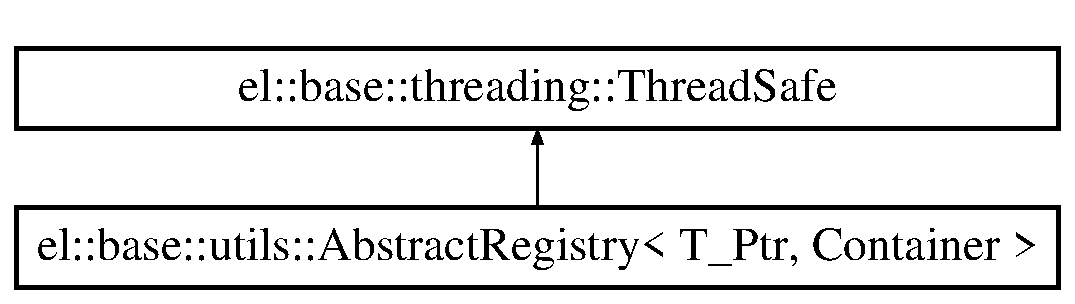
\includegraphics[height=2.000000cm]{classel_1_1base_1_1utils_1_1AbstractRegistry}
\end{center}
\end{figure}
\subsection*{Public Types}
\begin{DoxyCompactItemize}
\item 
\hypertarget{classel_1_1base_1_1utils_1_1AbstractRegistry_a58d0536c748633afd3f7c237b63a9a7c}{typedef Container\-::iterator {\bfseries iterator}}\label{classel_1_1base_1_1utils_1_1AbstractRegistry_a58d0536c748633afd3f7c237b63a9a7c}

\item 
\hypertarget{classel_1_1base_1_1utils_1_1AbstractRegistry_a3bbf19b112c067cb1a02a82b003cc7e2}{typedef Container\-::const\-\_\-iterator {\bfseries const\-\_\-iterator}}\label{classel_1_1base_1_1utils_1_1AbstractRegistry_a3bbf19b112c067cb1a02a82b003cc7e2}

\end{DoxyCompactItemize}
\subsection*{Public Member Functions}
\begin{DoxyCompactItemize}
\item 
\hypertarget{classel_1_1base_1_1utils_1_1AbstractRegistry_afe13c67ebd1ed1aa72845926894dffa2}{\hyperlink{classel_1_1base_1_1utils_1_1AbstractRegistry_afe13c67ebd1ed1aa72845926894dffa2}{Abstract\-Registry} (void)}\label{classel_1_1base_1_1utils_1_1AbstractRegistry_afe13c67ebd1ed1aa72845926894dffa2}

\begin{DoxyCompactList}\small\item\em Default constructor. \end{DoxyCompactList}\item 
\hypertarget{classel_1_1base_1_1utils_1_1AbstractRegistry_a9f468010439d491e90419f9334afcdba}{\hyperlink{classel_1_1base_1_1utils_1_1AbstractRegistry_a9f468010439d491e90419f9334afcdba}{Abstract\-Registry} (\hyperlink{classel_1_1base_1_1utils_1_1AbstractRegistry}{Abstract\-Registry} \&\&sr)}\label{classel_1_1base_1_1utils_1_1AbstractRegistry_a9f468010439d491e90419f9334afcdba}

\begin{DoxyCompactList}\small\item\em Move constructor that is useful for base classes. \end{DoxyCompactList}\item 
\hypertarget{classel_1_1base_1_1utils_1_1AbstractRegistry_ac3e648dc0caa8914f8604650f00bc94b}{bool {\bfseries operator==} (const \hyperlink{classel_1_1base_1_1utils_1_1AbstractRegistry}{Abstract\-Registry}$<$ T\-\_\-\-Ptr, Container $>$ \&other)}\label{classel_1_1base_1_1utils_1_1AbstractRegistry_ac3e648dc0caa8914f8604650f00bc94b}

\item 
\hypertarget{classel_1_1base_1_1utils_1_1AbstractRegistry_a35de8807521651c85acb26532a2623e1}{bool {\bfseries operator!=} (const \hyperlink{classel_1_1base_1_1utils_1_1AbstractRegistry}{Abstract\-Registry}$<$ T\-\_\-\-Ptr, Container $>$ \&other)}\label{classel_1_1base_1_1utils_1_1AbstractRegistry_a35de8807521651c85acb26532a2623e1}

\item 
\hypertarget{classel_1_1base_1_1utils_1_1AbstractRegistry_a5727a3cadeee6a2b10d8f46fb91956e7}{\hyperlink{classel_1_1base_1_1utils_1_1AbstractRegistry}{Abstract\-Registry} \& \hyperlink{classel_1_1base_1_1utils_1_1AbstractRegistry_a5727a3cadeee6a2b10d8f46fb91956e7}{operator=} (\hyperlink{classel_1_1base_1_1utils_1_1AbstractRegistry}{Abstract\-Registry} \&\&sr)}\label{classel_1_1base_1_1utils_1_1AbstractRegistry_a5727a3cadeee6a2b10d8f46fb91956e7}

\begin{DoxyCompactList}\small\item\em Assignment move operator. \end{DoxyCompactList}\item 
virtual iterator \hyperlink{classel_1_1base_1_1utils_1_1AbstractRegistry_a4ad971b1dddff996d327452d852e55b2}{begin} (void) E\-L\-P\-P\-\_\-\-F\-I\-N\-A\-L
\item 
virtual iterator \hyperlink{classel_1_1base_1_1utils_1_1AbstractRegistry_a67c40207c171f23ad50a71db819e84f9}{end} (void) E\-L\-P\-P\-\_\-\-F\-I\-N\-A\-L
\item 
virtual const\-\_\-iterator \hyperlink{classel_1_1base_1_1utils_1_1AbstractRegistry_a37f743184e808d7c0028e21e0d0898bb}{cbegin} (void) const E\-L\-P\-P\-\_\-\-F\-I\-N\-A\-L
\item 
virtual const\-\_\-iterator \hyperlink{classel_1_1base_1_1utils_1_1AbstractRegistry_ad3ee081b4b25c5d77f971f949bdb9158}{cend} (void) const E\-L\-P\-P\-\_\-\-F\-I\-N\-A\-L
\item 
virtual bool \hyperlink{classel_1_1base_1_1utils_1_1AbstractRegistry_a43ff6484b778c298416c482c07a4df3f}{empty} (void) const E\-L\-P\-P\-\_\-\-F\-I\-N\-A\-L
\item 
virtual std\-::size\-\_\-t \hyperlink{classel_1_1base_1_1utils_1_1AbstractRegistry_a58a7b8ea964bdf6008701dcfb6609ca5}{size} (void) const E\-L\-P\-P\-\_\-\-F\-I\-N\-A\-L
\item 
\hypertarget{classel_1_1base_1_1utils_1_1AbstractRegistry_a072859d3728a75f910c2898f62fd12da}{virtual Container \& \hyperlink{classel_1_1base_1_1utils_1_1AbstractRegistry_a072859d3728a75f910c2898f62fd12da}{list} (void) E\-L\-P\-P\-\_\-\-F\-I\-N\-A\-L}\label{classel_1_1base_1_1utils_1_1AbstractRegistry_a072859d3728a75f910c2898f62fd12da}

\begin{DoxyCompactList}\small\item\em Returns underlying container by reference. \end{DoxyCompactList}\item 
\hypertarget{classel_1_1base_1_1utils_1_1AbstractRegistry_a1c3da2af9177cbfae6f10b9e5dbe615c}{virtual const Container \& \hyperlink{classel_1_1base_1_1utils_1_1AbstractRegistry_a1c3da2af9177cbfae6f10b9e5dbe615c}{list} (void) const E\-L\-P\-P\-\_\-\-F\-I\-N\-A\-L}\label{classel_1_1base_1_1utils_1_1AbstractRegistry_a1c3da2af9177cbfae6f10b9e5dbe615c}

\begin{DoxyCompactList}\small\item\em Returns underlying container by constant reference. \end{DoxyCompactList}\item 
\hypertarget{classel_1_1base_1_1utils_1_1AbstractRegistry_a19223bc1fea48dbe6b47b4879aa4672f}{virtual void \hyperlink{classel_1_1base_1_1utils_1_1AbstractRegistry_a19223bc1fea48dbe6b47b4879aa4672f}{unregister\-All} (void)=0}\label{classel_1_1base_1_1utils_1_1AbstractRegistry_a19223bc1fea48dbe6b47b4879aa4672f}

\begin{DoxyCompactList}\small\item\em Unregisters all the pointers from current repository. \end{DoxyCompactList}\end{DoxyCompactItemize}
\subsection*{Protected Member Functions}
\begin{DoxyCompactItemize}
\item 
\hypertarget{classel_1_1base_1_1utils_1_1AbstractRegistry_aaf42dab7089a9b1198e2920983ca82bb}{virtual void {\bfseries deep\-Copy} (const \hyperlink{classel_1_1base_1_1utils_1_1AbstractRegistry}{Abstract\-Registry}$<$ T\-\_\-\-Ptr, Container $>$ \&)=0}\label{classel_1_1base_1_1utils_1_1AbstractRegistry_aaf42dab7089a9b1198e2920983ca82bb}

\item 
\hypertarget{classel_1_1base_1_1utils_1_1AbstractRegistry_a529677fb42e78d03c36cdea49f8877c9}{void {\bfseries reinit\-Deep\-Copy} (const \hyperlink{classel_1_1base_1_1utils_1_1AbstractRegistry}{Abstract\-Registry}$<$ T\-\_\-\-Ptr, Container $>$ \&sr)}\label{classel_1_1base_1_1utils_1_1AbstractRegistry_a529677fb42e78d03c36cdea49f8877c9}

\end{DoxyCompactItemize}


\subsection{Detailed Description}
\subsubsection*{template$<$typename T\-\_\-\-Ptr, typename Container$>$class el\-::base\-::utils\-::\-Abstract\-Registry$<$ T\-\_\-\-Ptr, Container $>$}

Abstract registry (aka repository) that provides basic interface for pointer repository specified by T\-\_\-\-Ptr type. 

Most of the functions are virtual final methods but anything implementing this abstract class should implement \hyperlink{classel_1_1base_1_1utils_1_1AbstractRegistry_a19223bc1fea48dbe6b47b4879aa4672f}{unregister\-All()} and deep\-Copy(const Abstract\-Registry$<$\-T\-\_\-\-Ptr, Container$>$\&) and write register\-New() method according to container and few more methods; get() to find element, unregister() to unregister single entry. Please note that this is thread-\/unsafe and should also implement thread-\/safety mechanisms in implementation. 

\subsection{Member Function Documentation}
\hypertarget{classel_1_1base_1_1utils_1_1AbstractRegistry_a4ad971b1dddff996d327452d852e55b2}{\index{el\-::base\-::utils\-::\-Abstract\-Registry@{el\-::base\-::utils\-::\-Abstract\-Registry}!begin@{begin}}
\index{begin@{begin}!el::base::utils::AbstractRegistry@{el\-::base\-::utils\-::\-Abstract\-Registry}}
\subsubsection[{begin}]{\setlength{\rightskip}{0pt plus 5cm}template$<$typename T\-\_\-\-Ptr, typename Container$>$ virtual iterator {\bf el\-::base\-::utils\-::\-Abstract\-Registry}$<$ T\-\_\-\-Ptr, Container $>$\-::begin (
\begin{DoxyParamCaption}
\item[{void}]{}
\end{DoxyParamCaption}
)\hspace{0.3cm}{\ttfamily [inline]}, {\ttfamily [virtual]}}}\label{classel_1_1base_1_1utils_1_1AbstractRegistry_a4ad971b1dddff996d327452d852e55b2}
\begin{DoxyReturn}{Returns}
Iterator pointer from start of repository 
\end{DoxyReturn}
\hypertarget{classel_1_1base_1_1utils_1_1AbstractRegistry_a37f743184e808d7c0028e21e0d0898bb}{\index{el\-::base\-::utils\-::\-Abstract\-Registry@{el\-::base\-::utils\-::\-Abstract\-Registry}!cbegin@{cbegin}}
\index{cbegin@{cbegin}!el::base::utils::AbstractRegistry@{el\-::base\-::utils\-::\-Abstract\-Registry}}
\subsubsection[{cbegin}]{\setlength{\rightskip}{0pt plus 5cm}template$<$typename T\-\_\-\-Ptr, typename Container$>$ virtual const\-\_\-iterator {\bf el\-::base\-::utils\-::\-Abstract\-Registry}$<$ T\-\_\-\-Ptr, Container $>$\-::cbegin (
\begin{DoxyParamCaption}
\item[{void}]{}
\end{DoxyParamCaption}
) const\hspace{0.3cm}{\ttfamily [inline]}, {\ttfamily [virtual]}}}\label{classel_1_1base_1_1utils_1_1AbstractRegistry_a37f743184e808d7c0028e21e0d0898bb}
\begin{DoxyReturn}{Returns}
Constant iterator pointer from start of repository 
\end{DoxyReturn}
\hypertarget{classel_1_1base_1_1utils_1_1AbstractRegistry_ad3ee081b4b25c5d77f971f949bdb9158}{\index{el\-::base\-::utils\-::\-Abstract\-Registry@{el\-::base\-::utils\-::\-Abstract\-Registry}!cend@{cend}}
\index{cend@{cend}!el::base::utils::AbstractRegistry@{el\-::base\-::utils\-::\-Abstract\-Registry}}
\subsubsection[{cend}]{\setlength{\rightskip}{0pt plus 5cm}template$<$typename T\-\_\-\-Ptr, typename Container$>$ virtual const\-\_\-iterator {\bf el\-::base\-::utils\-::\-Abstract\-Registry}$<$ T\-\_\-\-Ptr, Container $>$\-::cend (
\begin{DoxyParamCaption}
\item[{void}]{}
\end{DoxyParamCaption}
) const\hspace{0.3cm}{\ttfamily [inline]}, {\ttfamily [virtual]}}}\label{classel_1_1base_1_1utils_1_1AbstractRegistry_ad3ee081b4b25c5d77f971f949bdb9158}
\begin{DoxyReturn}{Returns}
End of repository 
\end{DoxyReturn}
\hypertarget{classel_1_1base_1_1utils_1_1AbstractRegistry_a43ff6484b778c298416c482c07a4df3f}{\index{el\-::base\-::utils\-::\-Abstract\-Registry@{el\-::base\-::utils\-::\-Abstract\-Registry}!empty@{empty}}
\index{empty@{empty}!el::base::utils::AbstractRegistry@{el\-::base\-::utils\-::\-Abstract\-Registry}}
\subsubsection[{empty}]{\setlength{\rightskip}{0pt plus 5cm}template$<$typename T\-\_\-\-Ptr, typename Container$>$ virtual bool {\bf el\-::base\-::utils\-::\-Abstract\-Registry}$<$ T\-\_\-\-Ptr, Container $>$\-::empty (
\begin{DoxyParamCaption}
\item[{void}]{}
\end{DoxyParamCaption}
) const\hspace{0.3cm}{\ttfamily [inline]}, {\ttfamily [virtual]}}}\label{classel_1_1base_1_1utils_1_1AbstractRegistry_a43ff6484b778c298416c482c07a4df3f}
\begin{DoxyReturn}{Returns}
Whether or not repository is empty 
\end{DoxyReturn}
\hypertarget{classel_1_1base_1_1utils_1_1AbstractRegistry_a67c40207c171f23ad50a71db819e84f9}{\index{el\-::base\-::utils\-::\-Abstract\-Registry@{el\-::base\-::utils\-::\-Abstract\-Registry}!end@{end}}
\index{end@{end}!el::base::utils::AbstractRegistry@{el\-::base\-::utils\-::\-Abstract\-Registry}}
\subsubsection[{end}]{\setlength{\rightskip}{0pt plus 5cm}template$<$typename T\-\_\-\-Ptr, typename Container$>$ virtual iterator {\bf el\-::base\-::utils\-::\-Abstract\-Registry}$<$ T\-\_\-\-Ptr, Container $>$\-::end (
\begin{DoxyParamCaption}
\item[{void}]{}
\end{DoxyParamCaption}
)\hspace{0.3cm}{\ttfamily [inline]}, {\ttfamily [virtual]}}}\label{classel_1_1base_1_1utils_1_1AbstractRegistry_a67c40207c171f23ad50a71db819e84f9}
\begin{DoxyReturn}{Returns}
Iterator pointer from end of repository 
\end{DoxyReturn}
\hypertarget{classel_1_1base_1_1utils_1_1AbstractRegistry_a58a7b8ea964bdf6008701dcfb6609ca5}{\index{el\-::base\-::utils\-::\-Abstract\-Registry@{el\-::base\-::utils\-::\-Abstract\-Registry}!size@{size}}
\index{size@{size}!el::base::utils::AbstractRegistry@{el\-::base\-::utils\-::\-Abstract\-Registry}}
\subsubsection[{size}]{\setlength{\rightskip}{0pt plus 5cm}template$<$typename T\-\_\-\-Ptr, typename Container$>$ virtual std\-::size\-\_\-t {\bf el\-::base\-::utils\-::\-Abstract\-Registry}$<$ T\-\_\-\-Ptr, Container $>$\-::size (
\begin{DoxyParamCaption}
\item[{void}]{}
\end{DoxyParamCaption}
) const\hspace{0.3cm}{\ttfamily [inline]}, {\ttfamily [virtual]}}}\label{classel_1_1base_1_1utils_1_1AbstractRegistry_a58a7b8ea964bdf6008701dcfb6609ca5}
\begin{DoxyReturn}{Returns}
Size of repository 
\end{DoxyReturn}


The documentation for this class was generated from the following file\-:\begin{DoxyCompactItemize}
\item 
/users/disk9/cfse/\-Stage\-\_\-\-Malo/\-C\-P\-A\-C\-S\-Creator\-Lib/\-C\-P\-A\-C\-S\-Creator\-Lib/easylogging++.\-h\end{DoxyCompactItemize}

\hypertarget{classcpcr_1_1AircraftTree}{\section{cpcr\-:\-:Aircraft\-Tree Class Reference}
\label{classcpcr_1_1AircraftTree}\index{cpcr\-::\-Aircraft\-Tree@{cpcr\-::\-Aircraft\-Tree}}
}
Inheritance diagram for cpcr\-:\-:Aircraft\-Tree\-:\begin{figure}[H]
\begin{center}
\leavevmode
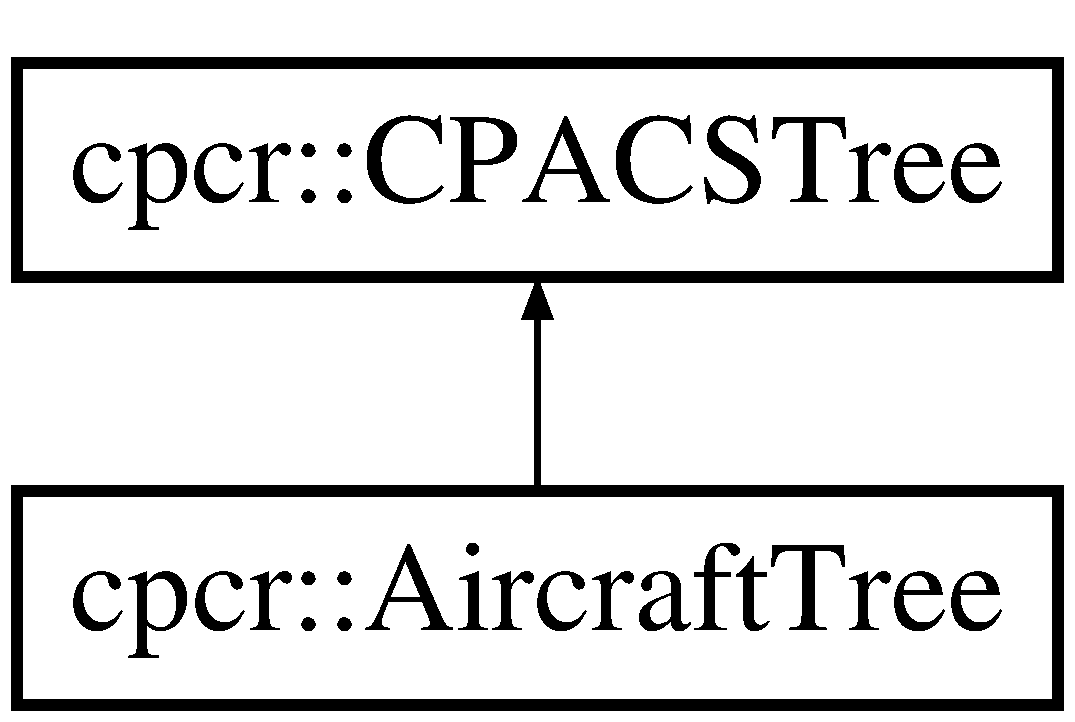
\includegraphics[height=2.000000cm]{classcpcr_1_1AircraftTree}
\end{center}
\end{figure}
\subsection*{Public Member Functions}
\begin{DoxyCompactItemize}
\item 
\hypertarget{classcpcr_1_1AircraftTree_ae744a2c510b2c41253a655b5b0dad2c7}{Tigl\-C\-P\-A\-C\-S\-Configuration\-Handle $\ast$ {\bfseries get\-Tigl\-Handle} ()}\label{classcpcr_1_1AircraftTree_ae744a2c510b2c41253a655b5b0dad2c7}

\item 
\hypertarget{classcpcr_1_1AircraftTree_ae014423054ed3f461d0a9f7dbc82d33b}{void {\bfseries build} (std\-::string file, \hyperlink{classcpcr_1_1UniqueXPath}{Unique\-X\-Path} root) override}\label{classcpcr_1_1AircraftTree_ae014423054ed3f461d0a9f7dbc82d33b}

\item 
\hypertarget{classcpcr_1_1AircraftTree_aee89f36aa0c2747c73610621c5ec7979}{void {\bfseries re\-Build} ()}\label{classcpcr_1_1AircraftTree_aee89f36aa0c2747c73610621c5ec7979}

\item 
\hypertarget{classcpcr_1_1AircraftTree_aa98b4e08584ca8b3afb96b1fb236a7dc}{void {\bfseries close} ()}\label{classcpcr_1_1AircraftTree_aa98b4e08584ca8b3afb96b1fb236a7dc}

\item 
\hypertarget{classcpcr_1_1AircraftTree_a076b3beaeb107a095ce2b6658620685e}{void {\bfseries write\-To\-File} ()}\label{classcpcr_1_1AircraftTree_a076b3beaeb107a095ce2b6658620685e}

\item 
\hypertarget{classcpcr_1_1AircraftTree_a0fbe75a07bbdfddcfb2bcd57fc9e4386}{void {\bfseries write\-To\-File} (std\-::string file\-Name)}\label{classcpcr_1_1AircraftTree_a0fbe75a07bbdfddcfb2bcd57fc9e4386}

\item 
\hypertarget{classcpcr_1_1AircraftTree_a5b84457be75ccd0296ca21fc19beddd3}{std\-::map$<$ \hyperlink{classcpcr_1_1CPACSTreeItem}{C\-P\-A\-C\-S\-Tree\-Item} \\*
$\ast$, std\-::vector$<$ \hyperlink{classcpcr_1_1CPACSTreeItem}{C\-P\-A\-C\-S\-Tree\-Item} $\ast$ $>$ $>$ {\bfseries get\-Wing\-Graph} (\hyperlink{classcpcr_1_1CPACSTreeItem}{C\-P\-A\-C\-S\-Tree\-Item} $\ast$wing)}\label{classcpcr_1_1AircraftTree_a5b84457be75ccd0296ca21fc19beddd3}

\item 
\hypertarget{classcpcr_1_1AircraftTree_ad663f9abc22df6d674e42fed3cd123d4}{std\-::vector$<$ \hyperlink{classcpcr_1_1CPACSTreeItem}{C\-P\-A\-C\-S\-Tree\-Item} $\ast$ $>$ {\bfseries format\-Graph} (std\-::map$<$ \hyperlink{classcpcr_1_1CPACSTreeItem}{C\-P\-A\-C\-S\-Tree\-Item} $\ast$, std\-::vector$<$ \hyperlink{classcpcr_1_1CPACSTreeItem}{C\-P\-A\-C\-S\-Tree\-Item} $\ast$ $>$ $>$ wing\-Graph)}\label{classcpcr_1_1AircraftTree_ad663f9abc22df6d674e42fed3cd123d4}

\item 
\hypertarget{classcpcr_1_1AircraftTree_a384681df8357d743335e41354e3a5de3}{void {\bfseries complete\-Standardization\-For\-Wing} (U\-I\-D wing\-U\-I\-D)}\label{classcpcr_1_1AircraftTree_a384681df8357d743335e41354e3a5de3}

\item 
\hypertarget{classcpcr_1_1AircraftTree_ae49297e508d07a2afa5811d7a6d9e736}{bool {\bfseries is\-Wing\-Standardized} (U\-I\-D wing\-U\-I\-D)}\label{classcpcr_1_1AircraftTree_ae49297e508d07a2afa5811d7a6d9e736}

\item 
\hypertarget{classcpcr_1_1AircraftTree_ab303a026eff60cb94cd8e3e5eaa9fa35}{bool {\bfseries check\-If\-Airfoils\-Are\-Standardized\-For\-Wing} (U\-I\-D wing\-U\-I\-D)}\label{classcpcr_1_1AircraftTree_ab303a026eff60cb94cd8e3e5eaa9fa35}

\item 
\hypertarget{classcpcr_1_1AircraftTree_ab0656d91ceb48d16d354c5b383bc0027}{void {\bfseries airfoils\-Standardization\-For\-Wing} (U\-I\-D wing\-U\-I\-D)}\label{classcpcr_1_1AircraftTree_ab0656d91ceb48d16d354c5b383bc0027}

\item 
\hypertarget{classcpcr_1_1AircraftTree_abb58f556c2ae1c4dc50c8a770a1c3da3}{bool {\bfseries check\-If\-Positionings\-Are\-Standardized\-For\-Wing} (U\-I\-D wing\-U\-I\-D)}\label{classcpcr_1_1AircraftTree_abb58f556c2ae1c4dc50c8a770a1c3da3}

\item 
\hypertarget{classcpcr_1_1AircraftTree_a9e73f854346e14316e4fec66823ee5b9}{void {\bfseries positionings\-Standardization\-For\-Wing} (U\-I\-D wing\-U\-I\-D)}\label{classcpcr_1_1AircraftTree_a9e73f854346e14316e4fec66823ee5b9}

\item 
\hypertarget{classcpcr_1_1AircraftTree_a9bb0c237f61252f8105037e09a466a56}{bool {\bfseries check\-If\-One\-Section\-One\-Element\-For\-Wing} (U\-I\-D wing\-U\-I\-D)}\label{classcpcr_1_1AircraftTree_a9bb0c237f61252f8105037e09a466a56}

\item 
void \hyperlink{classcpcr_1_1AircraftTree_acfdc292d3b13bbd05292a5812e2c6ed1}{one\-Section\-One\-Element\-Standardization\-For\-Wing} (U\-I\-D wing\-U\-I\-D)
\item 
\hypertarget{classcpcr_1_1AircraftTree_a62fa387d7ed3540cd82626addeeff672}{bool {\bfseries check\-If\-Wing\-Transformation\-Is\-Standardized\-For\-Wing} (U\-I\-D wing\-U\-I\-D)}\label{classcpcr_1_1AircraftTree_a62fa387d7ed3540cd82626addeeff672}

\item 
\hypertarget{classcpcr_1_1AircraftTree_aa3e27822a55e68d2c181a9fc626a0dcc}{void {\bfseries wing\-Transformation\-Standardization} (U\-I\-D wing\-U\-I\-D)}\label{classcpcr_1_1AircraftTree_aa3e27822a55e68d2c181a9fc626a0dcc}

\item 
\hypertarget{classcpcr_1_1AircraftTree_ade78abd6bb2b9ceedb5b86f0c167d598}{void {\bfseries set\-Wing\-Transformation} (U\-I\-D wing\-U\-I\-D, const \hyperlink{classcpcr_1_1CPACSTransformation}{C\-P\-A\-C\-S\-Transformation} \&new\-Transformation)}\label{classcpcr_1_1AircraftTree_ade78abd6bb2b9ceedb5b86f0c167d598}

\item 
\hyperlink{classcpcr_1_1CPACSTransformation}{C\-P\-A\-C\-S\-Transformation} \hyperlink{classcpcr_1_1AircraftTree_a1089f2cb81eed5db7f52c6342454ce5d}{determine\-Wing\-Transformation} (U\-I\-D wing\-U\-I\-D)
\item 
\hypertarget{classcpcr_1_1AircraftTree_a412b79ab38ba02069ea6fc68b433a77e}{void {\bfseries set\-Wing\-Airfoils\-From\-External\-File} (U\-I\-D wing\-U\-I\-D, std\-::string filename, bool keep\-Chord=true)}\label{classcpcr_1_1AircraftTree_a412b79ab38ba02069ea6fc68b433a77e}

\item 
void \hyperlink{classcpcr_1_1AircraftTree_afbbf121d2483d8fc793adeb4b22a5f59}{set\-Wing\-Airfoils\-By\-U\-I\-D} (U\-I\-D wing\-U\-I\-D, U\-I\-D airfoil\-U\-I\-D, bool keep\-Chord=true)
\item 
std\-::vector$<$ U\-I\-D $>$ \hyperlink{classcpcr_1_1AircraftTree_a6b7f9872f9a86e61ab998cc0e223972c}{get\-All\-Airfoils\-U\-I\-D\-In\-This\-Wing} (U\-I\-D wing\-U\-I\-D)
\item 
\hypertarget{classcpcr_1_1AircraftTree_a835d9dc570b3a85c4e15b367f84e057e}{double {\bfseries get\-Wing\-Dihedral} (U\-I\-D wing\-U\-I\-D, double chord\-Percent=0)}\label{classcpcr_1_1AircraftTree_a835d9dc570b3a85c4e15b367f84e057e}

\item 
\hypertarget{classcpcr_1_1AircraftTree_a2e875be685e1c4a4b208d02b19dfc1f1}{double {\bfseries get\-Wing\-World\-Dihedral} (U\-I\-D wing\-U\-I\-D, double chord\-Percent=0)}\label{classcpcr_1_1AircraftTree_a2e875be685e1c4a4b208d02b19dfc1f1}

\item 
\hypertarget{classcpcr_1_1AircraftTree_a4f11293a49e122411433d0ce55783c47}{void {\bfseries set\-Wing\-Dihedral} (U\-I\-D wing\-U\-I\-D, double dihedral, double chord\-Percent=0)}\label{classcpcr_1_1AircraftTree_a4f11293a49e122411433d0ce55783c47}

\item 
void \hyperlink{classcpcr_1_1AircraftTree_ad475604a92a2c9e4ad80f5b66a6bb852}{set\-Wing\-Symmetry} (U\-I\-D wing\-U\-I\-D, std\-::string)
\item 
std\-::string \hyperlink{classcpcr_1_1AircraftTree_a74e4ffc6b8581c9e9748cbec556b6fcc}{get\-Wing\-Symmetry} (U\-I\-D wing\-U\-I\-D)
\item 
double \hyperlink{classcpcr_1_1AircraftTree_aba201a5d66774e64cbaa7870087a73e1}{get\-Wing\-Sweep} (U\-I\-D wing\-U\-I\-D, double chord\-Percent=0)
\item 
void \hyperlink{classcpcr_1_1AircraftTree_ae7714bafa64d35000a0cfd299b4f954e}{set\-Wing\-Sweep\-By\-Translation} (U\-I\-D wing\-U\-I\-D, double sweep\-Angle, double chord\-Percent=0)
\item 
void \hyperlink{classcpcr_1_1AircraftTree_a4c2adb1082e02f7390a281c44868de8f}{set\-Wing\-Sweep\-By\-Shearing} (U\-I\-D wing\-U\-I\-D, double sweep\-Angle, double chord\-Percent=0)
\item 
Eigen\-::\-Matrix4d \hyperlink{classcpcr_1_1AircraftTree_a2404c22f8b1570b2600691506c60a965}{get\-Global\-Transform\-Matrix\-Of\-Element} (U\-I\-D element\-U\-I\-D)
\begin{DoxyCompactList}\small\item\em return the a matrix that represent all the affine transforms that is apply on the element \end{DoxyCompactList}\item 
std\-::vector$<$ std\-::pair\\*
$<$ \hyperlink{classcpcr_1_1CPACSTreeItem}{C\-P\-A\-C\-S\-Tree\-Item} \\*
$\ast$, Eigen\-::\-Matrix4d $>$ $>$ \hyperlink{classcpcr_1_1AircraftTree_ae9dc2df3ae532e7b6fe3124ba7d62ce0}{get\-Transformation\-Chain\-For\-One\-Element} (\hyperlink{classcpcr_1_1CPACSTreeItem}{C\-P\-A\-C\-S\-Tree\-Item} $\ast$element\-Item)
\item 
std\-::pair$<$ \hyperlink{classcpcr_1_1CPACSTreeItem}{C\-P\-A\-C\-S\-Tree\-Item} \\*
$\ast$, Eigen\-::\-Matrix4d $>$ \hyperlink{classcpcr_1_1AircraftTree_ae8b6aa1e5a1cee897160d54c596f9aba}{get\-Global\-Positioning\-Translation\-For\-Section} (U\-I\-D section\-U\-I\-D)
\item 
std\-::vector$<$ U\-I\-D $>$ \hyperlink{classcpcr_1_1AircraftTree_a53ffa4032bae96478332cba4fcce7710}{get\-All\-Element\-U\-I\-Ds\-Used\-In\-A\-Wing} (U\-I\-D wing\-U\-I\-D)
\begin{DoxyCompactList}\small\item\em Return once all the elements U\-I\-D used in this wing. \end{DoxyCompactList}\item 
std\-::map$<$ U\-I\-D, Eigen\-::\-Vector4d $>$ \hyperlink{classcpcr_1_1AircraftTree_a80bb2d4e67b22e7beeaca5f9a38571d3}{get\-Chord\-Points\-Of\-Elements} (U\-I\-D wing\-U\-I\-D, double Chord\-Percent)
\item 
\hyperlink{classcpcr_1_1CPACSTransformation}{C\-P\-A\-C\-S\-Transformation} \hyperlink{classcpcr_1_1AircraftTree_a354078d68acb6d647f4a373132f807f0}{get\-Transform\-To\-Place\-Element\-By\-Translation\-At} (const U\-I\-D \&element\-Uid, const Eigen\-::\-Vector4d \&wanted\-Origin\-P)
\begin{DoxyCompactList}\small\item\em Get the transform that the element U\-I\-D needed to have to be at the wanted position. This transform conserve the rotation and the scaling of the original one and change only the translation component. \end{DoxyCompactList}\item 
Eigen\-::\-Vector4d \hyperlink{classcpcr_1_1AircraftTree_a0888c4baf7f40e1f29003a73d81f0ae3}{compute\-Position\-To\-Have\-Sweep\-Angle} (Eigen\-::\-Vector4d origin\-P, Eigen\-::\-Vector4d to\-Place\-P, double sweep)
\item 
\hypertarget{classcpcr_1_1AircraftTree_aa6ae916d24a2efc9aa07be61b7802c80}{void {\bfseries create\-Wing} (U\-I\-D wing\-U\-I\-D, \hyperlink{classcpcr_1_1CPACSTransformation}{C\-P\-A\-C\-S\-Transformation} wing\-Anchor, std\-::vector$<$ \hyperlink{classcpcr_1_1CPACSPositioning}{C\-P\-A\-C\-S\-Positioning} $>$ positions, std\-::vector$<$ double $>$ sections\-Scaling, std\-::vector$<$ double $>$ elements\-Twist, std\-::vector$<$ U\-I\-D $>$ elements\-U\-I\-D)}\label{classcpcr_1_1AircraftTree_aa6ae916d24a2efc9aa07be61b7802c80}

\item 
\hypertarget{classcpcr_1_1AircraftTree_a9f109852b43b90a6e1db62be03109299}{double {\bfseries get\-Wing\-Planform\-Area\-By\-Tigl} (U\-I\-D wing\-Uid, Tigl\-Symmetry\-Axis symmetry\-Axis)}\label{classcpcr_1_1AircraftTree_a9f109852b43b90a6e1db62be03109299}

\item 
\hypertarget{classcpcr_1_1AircraftTree_ac00870b80a2edf024d923f82f9689e75}{Eigen\-::\-Vector4d {\bfseries compute\-Position\-To\-Have\-Dihedral\-Angle} (Eigen\-::\-Vector4d origin\-P, Eigen\-::\-Vector4d to\-Place\-P, double sweep)}\label{classcpcr_1_1AircraftTree_ac00870b80a2edf024d923f82f9689e75}

\item 
\hypertarget{classcpcr_1_1AircraftTree_abf7c650b9b2ee32eef65067de28a4bb3}{double {\bfseries get\-Wing\-Span} (U\-I\-D wing\-Uid, double chord\-Percent=0.\-0)}\label{classcpcr_1_1AircraftTree_abf7c650b9b2ee32eef65067de28a4bb3}

\item 
double \hyperlink{classcpcr_1_1AircraftTree_a6f25690ca6eb74160232a7e1db3f8067}{get\-Segment\-Area} (\hyperlink{classcpcr_1_1CPACSTreeItem}{C\-P\-A\-C\-S\-Tree\-Item} $\ast$segment, P\-L\-A\-N\-E)
\item 
double \hyperlink{classcpcr_1_1AircraftTree_a1f3cb361f72ecc148f44fd6ec7694109}{get\-Wing\-Planform\-Area} (U\-I\-D wing\-U\-I\-D, P\-L\-A\-N\-E)
\item 
\hypertarget{classcpcr_1_1AircraftTree_aecaa232b5b267b646a1bc61a168c6f4e}{double {\bfseries get\-Wing\-A\-R} (U\-I\-D wing\-U\-I\-D)}\label{classcpcr_1_1AircraftTree_aecaa232b5b267b646a1bc61a168c6f4e}

\item 
\hypertarget{classcpcr_1_1AircraftTree_ad50a708bfed8e22c805af14bd3ffee82}{void {\bfseries set\-Wing\-Span\-Keep\-Area} (U\-I\-D wing\-U\-I\-D, double new\-Span)}\label{classcpcr_1_1AircraftTree_ad50a708bfed8e22c805af14bd3ffee82}

\item 
\hypertarget{classcpcr_1_1AircraftTree_a43b1473aa8b38a6eb98c979b6445d22a}{void {\bfseries set\-Wing\-Span\-Keep\-A\-R} (U\-I\-D wing\-U\-I\-D, double new\-Span)}\label{classcpcr_1_1AircraftTree_a43b1473aa8b38a6eb98c979b6445d22a}

\item 
\hypertarget{classcpcr_1_1AircraftTree_ac907eb6252b2250163a513c7e35677fd}{void {\bfseries set\-Wing\-Area\-Keep\-Span} (U\-I\-D wing\-U\-I\-D, double new\-Half\-Span)}\label{classcpcr_1_1AircraftTree_ac907eb6252b2250163a513c7e35677fd}

\item 
\hypertarget{classcpcr_1_1AircraftTree_a8e1070996780f6322020fcb5c09aebbb}{void {\bfseries set\-Wing\-Area\-Keep\-A\-R} (U\-I\-D wing\-U\-I\-D, double new\-Half\-Span)}\label{classcpcr_1_1AircraftTree_a8e1070996780f6322020fcb5c09aebbb}

\item 
\hypertarget{classcpcr_1_1AircraftTree_acfdbf4b8105878bdb3ef0373a1f2c30d}{void {\bfseries set\-Wing\-A\-R\-Keep\-Span} (U\-I\-D wing\-U\-I\-D, double new\-Half\-Span)}\label{classcpcr_1_1AircraftTree_acfdbf4b8105878bdb3ef0373a1f2c30d}

\item 
\hypertarget{classcpcr_1_1AircraftTree_ad24012e546c82a53c247b77986258012}{void {\bfseries set\-Wing\-A\-R\-Keep\-Area} (U\-I\-D wing\-U\-I\-D, double new\-Half\-Span)}\label{classcpcr_1_1AircraftTree_ad24012e546c82a53c247b77986258012}

\end{DoxyCompactItemize}
\subsection*{Protected Member Functions}
\begin{DoxyCompactItemize}
\item 
\hypertarget{classcpcr_1_1AircraftTree_a49200cf63bc3875e7634357d0576dfcf}{void {\bfseries set\-Wing\-Airfoils\-By\-U\-I\-D\-Keep\-Chord} (\hyperlink{classcpcr_1_1CPACSTreeItem}{C\-P\-A\-C\-S\-Tree\-Item} $\ast$wing, U\-I\-D airfoil\-U\-I\-D)}\label{classcpcr_1_1AircraftTree_a49200cf63bc3875e7634357d0576dfcf}

\item 
\hypertarget{classcpcr_1_1AircraftTree_ac3ac46fa7321d6cb85eb976de0e1905d}{void {\bfseries set\-Wing\-Airfoils\-By\-U\-I\-D\-Basic} (\hyperlink{classcpcr_1_1CPACSTreeItem}{C\-P\-A\-C\-S\-Tree\-Item} $\ast$wing, U\-I\-D airfoil\-U\-I\-D)}\label{classcpcr_1_1AircraftTree_ac3ac46fa7321d6cb85eb976de0e1905d}

\item 
\hypertarget{classcpcr_1_1AircraftTree_a599d0ce228bb15db40e292417e13b872}{U\-I\-D {\bfseries get\-Root\-Of\-Wing} (\hyperlink{classcpcr_1_1CPACSTreeItem}{C\-P\-A\-C\-S\-Tree\-Item} $\ast$wing)}\label{classcpcr_1_1AircraftTree_a599d0ce228bb15db40e292417e13b872}

\item 
\hypertarget{classcpcr_1_1AircraftTree_a046f619d04c98bab6d04674271434035}{U\-I\-D {\bfseries get\-Extremity\-In\-Y} (cpcr\-::\-U\-I\-D root\-U\-I\-D, std\-::map$<$ cpcr\-::\-U\-I\-D, Eigen\-::\-Vector4d $>$)}\label{classcpcr_1_1AircraftTree_a046f619d04c98bab6d04674271434035}

\item 
\hypertarget{classcpcr_1_1AircraftTree_aee6abd453fb7b2ce063df47586adf99d}{void {\bfseries place\-Element\-Minimal\-Changes} (\hyperlink{classcpcr_1_1CPACSTreeItem}{C\-P\-A\-C\-S\-Tree\-Item} $\ast$element, Eigen\-::\-Matrix4d global\-M)}\label{classcpcr_1_1AircraftTree_aee6abd453fb7b2ce063df47586adf99d}

\item 
\hypertarget{classcpcr_1_1AircraftTree_ace86833969231ac0e2c5043b9b3fa3b2}{void {\bfseries place\-Element\-Respect\-Std} (\hyperlink{classcpcr_1_1CPACSTreeItem}{C\-P\-A\-C\-S\-Tree\-Item} $\ast$element, Eigen\-::\-Matrix4d global\-M)}\label{classcpcr_1_1AircraftTree_ace86833969231ac0e2c5043b9b3fa3b2}

\item 
void \hyperlink{classcpcr_1_1AircraftTree_aff7e38fe83c5c04be75d5991ea6af226}{place\-Element} (\hyperlink{classcpcr_1_1CPACSTreeItem}{C\-P\-A\-C\-S\-Tree\-Item} $\ast$element, Eigen\-::\-Matrix4d global\-M)
\item 
\hypertarget{classcpcr_1_1AircraftTree_adabbf01ccf31be1d7dd8e6423015a09e}{void {\bfseries open\-Tigl\-Handle} (std\-::string model\-Uid)}\label{classcpcr_1_1AircraftTree_adabbf01ccf31be1d7dd8e6423015a09e}

\item 
\hypertarget{classcpcr_1_1AircraftTree_a5d0c0426ef6af0696f8b28a2146755bb}{void {\bfseries close\-Tigl\-Handle} ()}\label{classcpcr_1_1AircraftTree_a5d0c0426ef6af0696f8b28a2146755bb}

\end{DoxyCompactItemize}
\subsection*{Additional Inherited Members}


\subsection{Member Function Documentation}
\hypertarget{classcpcr_1_1AircraftTree_a0888c4baf7f40e1f29003a73d81f0ae3}{\index{cpcr\-::\-Aircraft\-Tree@{cpcr\-::\-Aircraft\-Tree}!compute\-Position\-To\-Have\-Sweep\-Angle@{compute\-Position\-To\-Have\-Sweep\-Angle}}
\index{compute\-Position\-To\-Have\-Sweep\-Angle@{compute\-Position\-To\-Have\-Sweep\-Angle}!cpcr::AircraftTree@{cpcr\-::\-Aircraft\-Tree}}
\subsubsection[{compute\-Position\-To\-Have\-Sweep\-Angle}]{\setlength{\rightskip}{0pt plus 5cm}Eigen\-::\-Vector4d cpcr\-::\-Aircraft\-Tree\-::compute\-Position\-To\-Have\-Sweep\-Angle (
\begin{DoxyParamCaption}
\item[{Eigen\-::\-Vector4d}]{origin\-P, }
\item[{Eigen\-::\-Vector4d}]{to\-Place\-P, }
\item[{double}]{sweep}
\end{DoxyParamCaption}
)}}\label{classcpcr_1_1AircraftTree_a0888c4baf7f40e1f29003a73d81f0ae3}
Return a new vector that has a angle of \char`\"{}sweep\-Angle\char`\"{} with the given origin vector. This mean that the new vector as the same y and z coordinate as the \char`\"{}to\-Place\-P\char`\"{} vector, but the x coordinate is such that the angle on the X\-Y-\/plan is equal to \char`\"{}sweep\-Angle\char`\"{}


\begin{DoxyParams}{Parameters}
{\em origin\-P} & \\
\hline
{\em to\-Place\-P} & \\
\hline
{\em sweep} & \\
\hline
\end{DoxyParams}
\begin{DoxyReturn}{Returns}
the new vector 
\end{DoxyReturn}
\hypertarget{classcpcr_1_1AircraftTree_a1089f2cb81eed5db7f52c6342454ce5d}{\index{cpcr\-::\-Aircraft\-Tree@{cpcr\-::\-Aircraft\-Tree}!determine\-Wing\-Transformation@{determine\-Wing\-Transformation}}
\index{determine\-Wing\-Transformation@{determine\-Wing\-Transformation}!cpcr::AircraftTree@{cpcr\-::\-Aircraft\-Tree}}
\subsubsection[{determine\-Wing\-Transformation}]{\setlength{\rightskip}{0pt plus 5cm}{\bf cpcr\-::\-C\-P\-A\-C\-S\-Transformation} cpcr\-::\-Aircraft\-Tree\-::determine\-Wing\-Transformation (
\begin{DoxyParamCaption}
\item[{U\-I\-D}]{wing\-U\-I\-D}
\end{DoxyParamCaption}
)}}\label{classcpcr_1_1AircraftTree_a1089f2cb81eed5db7f52c6342454ce5d}
Evaluate which transform is more adapted for the wing. 1) The origin of the transform is postionned (by translation) to the leading edge of the root element. 2) If the wing seems to be on the X\-Z plane (global dihedral higher than 45 degree), a transformation of 90 degree around X seems appropriate. Otherwise no rotation is perform on the wing.


\begin{DoxyParams}{Parameters}
{\em wing} & \\
\hline
\end{DoxyParams}
\begin{DoxyReturn}{Returns}
The new standardized transformation 
\end{DoxyReturn}
\hypertarget{classcpcr_1_1AircraftTree_a6b7f9872f9a86e61ab998cc0e223972c}{\index{cpcr\-::\-Aircraft\-Tree@{cpcr\-::\-Aircraft\-Tree}!get\-All\-Airfoils\-U\-I\-D\-In\-This\-Wing@{get\-All\-Airfoils\-U\-I\-D\-In\-This\-Wing}}
\index{get\-All\-Airfoils\-U\-I\-D\-In\-This\-Wing@{get\-All\-Airfoils\-U\-I\-D\-In\-This\-Wing}!cpcr::AircraftTree@{cpcr\-::\-Aircraft\-Tree}}
\subsubsection[{get\-All\-Airfoils\-U\-I\-D\-In\-This\-Wing}]{\setlength{\rightskip}{0pt plus 5cm}std\-::vector$<$ cpcr\-::\-U\-I\-D $>$ cpcr\-::\-Aircraft\-Tree\-::get\-All\-Airfoils\-U\-I\-D\-In\-This\-Wing (
\begin{DoxyParamCaption}
\item[{cpcr\-::\-U\-I\-D}]{wing\-U\-I\-D}
\end{DoxyParamCaption}
)}}\label{classcpcr_1_1AircraftTree_a6b7f9872f9a86e61ab998cc0e223972c}
Return the wing airfoil uid used by the wing given as parameter. If the same airfoil is used by multiples elements, the vector will contains this uid only once; If a airfoil uid is in a element but this element is not used in any segment, the airfoil uid will not be present 
\begin{DoxyParams}{Parameters}
{\em wing\-U\-I\-D,\-:} & the analyzed wing \\
\hline
\end{DoxyParams}
\begin{DoxyReturn}{Returns}
the list of used uid 
\end{DoxyReturn}
\hypertarget{classcpcr_1_1AircraftTree_a53ffa4032bae96478332cba4fcce7710}{\index{cpcr\-::\-Aircraft\-Tree@{cpcr\-::\-Aircraft\-Tree}!get\-All\-Element\-U\-I\-Ds\-Used\-In\-A\-Wing@{get\-All\-Element\-U\-I\-Ds\-Used\-In\-A\-Wing}}
\index{get\-All\-Element\-U\-I\-Ds\-Used\-In\-A\-Wing@{get\-All\-Element\-U\-I\-Ds\-Used\-In\-A\-Wing}!cpcr::AircraftTree@{cpcr\-::\-Aircraft\-Tree}}
\subsubsection[{get\-All\-Element\-U\-I\-Ds\-Used\-In\-A\-Wing}]{\setlength{\rightskip}{0pt plus 5cm}std\-::vector$<$ cpcr\-::\-U\-I\-D $>$ cpcr\-::\-Aircraft\-Tree\-::get\-All\-Element\-U\-I\-Ds\-Used\-In\-A\-Wing (
\begin{DoxyParamCaption}
\item[{U\-I\-D}]{wing\-U\-I\-D}
\end{DoxyParamCaption}
)}}\label{classcpcr_1_1AircraftTree_a53ffa4032bae96478332cba4fcce7710}


Return once all the elements U\-I\-D used in this wing. 


\begin{DoxyParams}{Parameters}
{\em wing\-U\-I\-D} & \\
\hline
\end{DoxyParams}
\begin{DoxyReturn}{Returns}
a vector of U\-I\-D
\end{DoxyReturn}
All U\-I\-D contained in \char`\"{}from\-Element\-U\-I\-D\char`\"{} and \char`\"{}to\-Element\-U\-I\-D\char`\"{} in the \char`\"{}segments\char`\"{} of this wing are extracted. Then a vector that contains exactly each U\-I\-D once is returned. \hypertarget{classcpcr_1_1AircraftTree_a80bb2d4e67b22e7beeaca5f9a38571d3}{\index{cpcr\-::\-Aircraft\-Tree@{cpcr\-::\-Aircraft\-Tree}!get\-Chord\-Points\-Of\-Elements@{get\-Chord\-Points\-Of\-Elements}}
\index{get\-Chord\-Points\-Of\-Elements@{get\-Chord\-Points\-Of\-Elements}!cpcr::AircraftTree@{cpcr\-::\-Aircraft\-Tree}}
\subsubsection[{get\-Chord\-Points\-Of\-Elements}]{\setlength{\rightskip}{0pt plus 5cm}std\-::map$<$ cpcr\-::\-U\-I\-D, Eigen\-::\-Vector4d $>$ cpcr\-::\-Aircraft\-Tree\-::get\-Chord\-Points\-Of\-Elements (
\begin{DoxyParamCaption}
\item[{cpcr\-::\-U\-I\-D}]{wing\-U\-I\-D, }
\item[{double}]{Chord\-Percent}
\end{DoxyParamCaption}
)}}\label{classcpcr_1_1AircraftTree_a80bb2d4e67b22e7beeaca5f9a38571d3}
Retrieve form T\-I\-G\-L the chord position of every element in a wing 
\begin{DoxyParams}{Parameters}
{\em wing\-U\-I\-D} & \\
\hline
{\em Chord\-Percent} & (0\-: Leading edge, 1\-: trailing edge) \\
\hline
\end{DoxyParams}
\begin{DoxyReturn}{Returns}

\end{DoxyReturn}
\hypertarget{classcpcr_1_1AircraftTree_ae8b6aa1e5a1cee897160d54c596f9aba}{\index{cpcr\-::\-Aircraft\-Tree@{cpcr\-::\-Aircraft\-Tree}!get\-Global\-Positioning\-Translation\-For\-Section@{get\-Global\-Positioning\-Translation\-For\-Section}}
\index{get\-Global\-Positioning\-Translation\-For\-Section@{get\-Global\-Positioning\-Translation\-For\-Section}!cpcr::AircraftTree@{cpcr\-::\-Aircraft\-Tree}}
\subsubsection[{get\-Global\-Positioning\-Translation\-For\-Section}]{\setlength{\rightskip}{0pt plus 5cm}std\-::pair$<$ {\bf cpcr\-::\-C\-P\-A\-C\-S\-Tree\-Item} $\ast$, Eigen\-::\-Matrix4d $>$ cpcr\-::\-Aircraft\-Tree\-::get\-Global\-Positioning\-Translation\-For\-Section (
\begin{DoxyParamCaption}
\item[{cpcr\-::\-U\-I\-D}]{section\-U\-I\-D}
\end{DoxyParamCaption}
)}}\label{classcpcr_1_1AircraftTree_ae8b6aa1e5a1cee897160d54c596f9aba}
Get the global translation that the section get from Positionings elements. This means basically, that all the implicit references of the \char`\"{}from\-Section\-U\-I\-D\char`\"{} of positionings are elucidate and added in the global translation. 
\begin{DoxyParams}{Parameters}
{\em section} & element \\
\hline
\end{DoxyParams}
\begin{DoxyReturn}{Returns}
main positioning tree item element and global translation matrix in world coordinate 
\end{DoxyReturn}
\hypertarget{classcpcr_1_1AircraftTree_a2404c22f8b1570b2600691506c60a965}{\index{cpcr\-::\-Aircraft\-Tree@{cpcr\-::\-Aircraft\-Tree}!get\-Global\-Transform\-Matrix\-Of\-Element@{get\-Global\-Transform\-Matrix\-Of\-Element}}
\index{get\-Global\-Transform\-Matrix\-Of\-Element@{get\-Global\-Transform\-Matrix\-Of\-Element}!cpcr::AircraftTree@{cpcr\-::\-Aircraft\-Tree}}
\subsubsection[{get\-Global\-Transform\-Matrix\-Of\-Element}]{\setlength{\rightskip}{0pt plus 5cm}Eigen\-::\-Matrix4d cpcr\-::\-Aircraft\-Tree\-::get\-Global\-Transform\-Matrix\-Of\-Element (
\begin{DoxyParamCaption}
\item[{U\-I\-D}]{element\-U\-I\-D}
\end{DoxyParamCaption}
)}}\label{classcpcr_1_1AircraftTree_a2404c22f8b1570b2600691506c60a965}


return the a matrix that represent all the affine transforms that is apply on the element 


\begin{DoxyParams}{Parameters}
{\em element\-U\-I\-D} & \\
\hline
{\em wing\-Item} & \\
\hline
\end{DoxyParams}
\begin{DoxyReturn}{Returns}
an Affine 4\-D matrix 
\end{DoxyReturn}
\hypertarget{classcpcr_1_1AircraftTree_a6f25690ca6eb74160232a7e1db3f8067}{\index{cpcr\-::\-Aircraft\-Tree@{cpcr\-::\-Aircraft\-Tree}!get\-Segment\-Area@{get\-Segment\-Area}}
\index{get\-Segment\-Area@{get\-Segment\-Area}!cpcr::AircraftTree@{cpcr\-::\-Aircraft\-Tree}}
\subsubsection[{get\-Segment\-Area}]{\setlength{\rightskip}{0pt plus 5cm}double cpcr\-::\-Aircraft\-Tree\-::get\-Segment\-Area (
\begin{DoxyParamCaption}
\item[{{\bf cpcr\-::\-C\-P\-A\-C\-S\-Tree\-Item} $\ast$}]{segment\-Item, }
\item[{P\-L\-A\-N\-E}]{plane}
\end{DoxyParamCaption}
)}}\label{classcpcr_1_1AircraftTree_a6f25690ca6eb74160232a7e1db3f8067}
Get the area of the segment in the wing coordinate system.


\begin{DoxyParams}{Parameters}
{\em segment} & \\
\hline
\end{DoxyParams}
\begin{DoxyReturn}{Returns}

\end{DoxyReturn}
\hypertarget{classcpcr_1_1AircraftTree_ae9dc2df3ae532e7b6fe3124ba7d62ce0}{\index{cpcr\-::\-Aircraft\-Tree@{cpcr\-::\-Aircraft\-Tree}!get\-Transformation\-Chain\-For\-One\-Element@{get\-Transformation\-Chain\-For\-One\-Element}}
\index{get\-Transformation\-Chain\-For\-One\-Element@{get\-Transformation\-Chain\-For\-One\-Element}!cpcr::AircraftTree@{cpcr\-::\-Aircraft\-Tree}}
\subsubsection[{get\-Transformation\-Chain\-For\-One\-Element}]{\setlength{\rightskip}{0pt plus 5cm}std\-::vector$<$ std\-::pair$<$ {\bf cpcr\-::\-C\-P\-A\-C\-S\-Tree\-Item} $\ast$, Eigen\-::\-Matrix4d $>$ $>$ cpcr\-::\-Aircraft\-Tree\-::get\-Transformation\-Chain\-For\-One\-Element (
\begin{DoxyParamCaption}
\item[{{\bf cpcr\-::\-C\-P\-A\-C\-S\-Tree\-Item} $\ast$}]{element\-Item}
\end{DoxyParamCaption}
)}}\label{classcpcr_1_1AircraftTree_ae9dc2df3ae532e7b6fe3124ba7d62ce0}
Get all the tree\-Items that can influence the position of the C\-P\-A\-C\-S\-Element given as parameter. This means that all the Transformation and Positioning that influence this particular element are returned as a vector composed of pair of the form $<$Tree\-Item$\ast$, Matrix4d$>$. The Matrix4d represent the transformation in the world coordinate. The first pair of the vector is the first transformation apply on the C\-P\-A\-C\-S\-Element and the last pair is the last transformation apply on the C\-P\-A\-C\-S\-Element. So we get the 4 matrices\-:

\mbox{[}0\mbox{]} Element matrix \mbox{[}1\mbox{]} Section matrix \mbox{[}2\mbox{]} Positioning matrix \mbox{[}3\mbox{]} Wing matrix


\begin{DoxyParams}{Parameters}
{\em element\-Tree\-Item} & \\
\hline
\end{DoxyParams}
\begin{DoxyReturn}{Returns}
vector of transformations 
\end{DoxyReturn}
\hypertarget{classcpcr_1_1AircraftTree_a354078d68acb6d647f4a373132f807f0}{\index{cpcr\-::\-Aircraft\-Tree@{cpcr\-::\-Aircraft\-Tree}!get\-Transform\-To\-Place\-Element\-By\-Translation\-At@{get\-Transform\-To\-Place\-Element\-By\-Translation\-At}}
\index{get\-Transform\-To\-Place\-Element\-By\-Translation\-At@{get\-Transform\-To\-Place\-Element\-By\-Translation\-At}!cpcr::AircraftTree@{cpcr\-::\-Aircraft\-Tree}}
\subsubsection[{get\-Transform\-To\-Place\-Element\-By\-Translation\-At}]{\setlength{\rightskip}{0pt plus 5cm}{\bf cpcr\-::\-C\-P\-A\-C\-S\-Transformation} cpcr\-::\-Aircraft\-Tree\-::get\-Transform\-To\-Place\-Element\-By\-Translation\-At (
\begin{DoxyParamCaption}
\item[{const U\-I\-D \&}]{element\-Uid, }
\item[{const Eigen\-::\-Vector4d \&}]{wanted\-Origin\-P}
\end{DoxyParamCaption}
)}}\label{classcpcr_1_1AircraftTree_a354078d68acb6d647f4a373132f807f0}


Get the transform that the element U\-I\-D needed to have to be at the wanted position. This transform conserve the rotation and the scaling of the original one and change only the translation component. 


\begin{DoxyParams}{Parameters}
{\em element\-Uid} & uid of the element to place \\
\hline
{\em wanted\-Origin\-P} & the wanted origin position for the element \\
\hline
\end{DoxyParams}
\begin{DoxyReturn}{Returns}
C\-P\-A\-C\-S\-Transform that the element should have to be at the wanted position 
\end{DoxyReturn}
\hypertarget{classcpcr_1_1AircraftTree_a1f3cb361f72ecc148f44fd6ec7694109}{\index{cpcr\-::\-Aircraft\-Tree@{cpcr\-::\-Aircraft\-Tree}!get\-Wing\-Planform\-Area@{get\-Wing\-Planform\-Area}}
\index{get\-Wing\-Planform\-Area@{get\-Wing\-Planform\-Area}!cpcr::AircraftTree@{cpcr\-::\-Aircraft\-Tree}}
\subsubsection[{get\-Wing\-Planform\-Area}]{\setlength{\rightskip}{0pt plus 5cm}double cpcr\-::\-Aircraft\-Tree\-::get\-Wing\-Planform\-Area (
\begin{DoxyParamCaption}
\item[{cpcr\-::\-U\-I\-D}]{wing\-U\-I\-D, }
\item[{cpcr\-::\-P\-L\-A\-N\-E}]{plane}
\end{DoxyParamCaption}
)}}\label{classcpcr_1_1AircraftTree_a1f3cb361f72ecc148f44fd6ec7694109}
Get the planforme area in the wing coordinate system'. 
\begin{DoxyParams}{Parameters}
{\em wing\-U\-I\-D} & \\
\hline
\end{DoxyParams}
\begin{DoxyReturn}{Returns}

\end{DoxyReturn}
\hypertarget{classcpcr_1_1AircraftTree_aba201a5d66774e64cbaa7870087a73e1}{\index{cpcr\-::\-Aircraft\-Tree@{cpcr\-::\-Aircraft\-Tree}!get\-Wing\-Sweep@{get\-Wing\-Sweep}}
\index{get\-Wing\-Sweep@{get\-Wing\-Sweep}!cpcr::AircraftTree@{cpcr\-::\-Aircraft\-Tree}}
\subsubsection[{get\-Wing\-Sweep}]{\setlength{\rightskip}{0pt plus 5cm}double cpcr\-::\-Aircraft\-Tree\-::get\-Wing\-Sweep (
\begin{DoxyParamCaption}
\item[{cpcr\-::\-U\-I\-D}]{wing\-U\-I\-D, }
\item[{double}]{chord\-Percent = {\ttfamily 0}}
\end{DoxyParamCaption}
)}}\label{classcpcr_1_1AircraftTree_aba201a5d66774e64cbaa7870087a73e1}
Get the sweep angle of the wing using the given chord percent or the the leading (chord percent = 0) by default.


\begin{DoxyParams}{Parameters}
{\em wing\-U\-I\-D} & \\
\hline
{\em chord\-Percent} & the percentage of the chord to use for computing the sweep angle. A percentage of 0 means taht we take the leading edge and a percent of 1 means that we take the trailing edge \\
\hline
\end{DoxyParams}
\begin{DoxyReturn}{Returns}
sweep angle 
\end{DoxyReturn}
\begin{DoxyRemark}{Remarks}
This method use tigl3 to get the position of the point on the chord. 
\end{DoxyRemark}
\hypertarget{classcpcr_1_1AircraftTree_a74e4ffc6b8581c9e9748cbec556b6fcc}{\index{cpcr\-::\-Aircraft\-Tree@{cpcr\-::\-Aircraft\-Tree}!get\-Wing\-Symmetry@{get\-Wing\-Symmetry}}
\index{get\-Wing\-Symmetry@{get\-Wing\-Symmetry}!cpcr::AircraftTree@{cpcr\-::\-Aircraft\-Tree}}
\subsubsection[{get\-Wing\-Symmetry}]{\setlength{\rightskip}{0pt plus 5cm}std\-::string cpcr\-::\-Aircraft\-Tree\-::get\-Wing\-Symmetry (
\begin{DoxyParamCaption}
\item[{cpcr\-::\-U\-I\-D}]{wing\-U\-I\-D}
\end{DoxyParamCaption}
)}}\label{classcpcr_1_1AircraftTree_a74e4ffc6b8581c9e9748cbec556b6fcc}
Retrieve the symmetry attribute of the wing. 
\begin{DoxyParams}{Parameters}
{\em wing\-U\-I\-D} & \\
\hline
\end{DoxyParams}
\hypertarget{classcpcr_1_1AircraftTree_acfdc292d3b13bbd05292a5812e2c6ed1}{\index{cpcr\-::\-Aircraft\-Tree@{cpcr\-::\-Aircraft\-Tree}!one\-Section\-One\-Element\-Standardization\-For\-Wing@{one\-Section\-One\-Element\-Standardization\-For\-Wing}}
\index{one\-Section\-One\-Element\-Standardization\-For\-Wing@{one\-Section\-One\-Element\-Standardization\-For\-Wing}!cpcr::AircraftTree@{cpcr\-::\-Aircraft\-Tree}}
\subsubsection[{one\-Section\-One\-Element\-Standardization\-For\-Wing}]{\setlength{\rightskip}{0pt plus 5cm}void cpcr\-::\-Aircraft\-Tree\-::one\-Section\-One\-Element\-Standardization\-For\-Wing (
\begin{DoxyParamCaption}
\item[{U\-I\-D}]{wing\-U\-I\-D}
\end{DoxyParamCaption}
)}}\label{classcpcr_1_1AircraftTree_acfdc292d3b13bbd05292a5812e2c6ed1}
Create one section for each element.

\begin{DoxyRemark}{Remarks}
The aircraft tree will be save in file and rebuild, all the \hyperlink{classcpcr_1_1CPACSTreeItem}{C\-P\-A\-C\-S\-Tree\-Item} will change !!!!!!!!! 
\end{DoxyRemark}

\begin{DoxyParams}{Parameters}
{\em wing} & \\
\hline
\end{DoxyParams}
\hypertarget{classcpcr_1_1AircraftTree_aff7e38fe83c5c04be75d5991ea6af226}{\index{cpcr\-::\-Aircraft\-Tree@{cpcr\-::\-Aircraft\-Tree}!place\-Element@{place\-Element}}
\index{place\-Element@{place\-Element}!cpcr::AircraftTree@{cpcr\-::\-Aircraft\-Tree}}
\subsubsection[{place\-Element}]{\setlength{\rightskip}{0pt plus 5cm}void cpcr\-::\-Aircraft\-Tree\-::place\-Element (
\begin{DoxyParamCaption}
\item[{{\bf cpcr\-::\-C\-P\-A\-C\-S\-Tree\-Item} $\ast$}]{element, }
\item[{Eigen\-::\-Matrix4d}]{global\-M}
\end{DoxyParamCaption}
)\hspace{0.3cm}{\ttfamily [protected]}}}\label{classcpcr_1_1AircraftTree_aff7e38fe83c5c04be75d5991ea6af226}
This function set the cpacs tree such that the given element ended with a the given global matrix. If the wing seems to respect the creator standard the function will try to keep the creator standard. Otherwise it will chang has less as possible the file. This mean that the only element transformation will be changed.

\begin{DoxyRemark}{Remarks}
The element becomes dependent of other element though positioning. Thus if this function is used to place multiples elements the order of the call is important.
\end{DoxyRemark}

\begin{DoxyParams}{Parameters}
{\em element} & \\
\hline
{\em global\-M} & \\
\hline
\end{DoxyParams}
\hypertarget{classcpcr_1_1AircraftTree_afbbf121d2483d8fc793adeb4b22a5f59}{\index{cpcr\-::\-Aircraft\-Tree@{cpcr\-::\-Aircraft\-Tree}!set\-Wing\-Airfoils\-By\-U\-I\-D@{set\-Wing\-Airfoils\-By\-U\-I\-D}}
\index{set\-Wing\-Airfoils\-By\-U\-I\-D@{set\-Wing\-Airfoils\-By\-U\-I\-D}!cpcr::AircraftTree@{cpcr\-::\-Aircraft\-Tree}}
\subsubsection[{set\-Wing\-Airfoils\-By\-U\-I\-D}]{\setlength{\rightskip}{0pt plus 5cm}void cpcr\-::\-Aircraft\-Tree\-::set\-Wing\-Airfoils\-By\-U\-I\-D (
\begin{DoxyParamCaption}
\item[{cpcr\-::\-U\-I\-D}]{wing\-U\-I\-D, }
\item[{cpcr\-::\-U\-I\-D}]{airfoil\-U\-I\-D, }
\item[{bool}]{keep\-Chord = {\ttfamily true}}
\end{DoxyParamCaption}
)}}\label{classcpcr_1_1AircraftTree_afbbf121d2483d8fc793adeb4b22a5f59}
Change all the airfoil used by this wing. The airfoil must already by present in the C\-P\-A\-C\-S file, if not a error is throw.


\begin{DoxyParams}{Parameters}
{\em wing\-U\-I\-D} & \-: the wing that will use this airfoil \\
\hline
{\em airfoil\-U\-I\-D} & \-: the airfoil U\-I\-D to be used \\
\hline
{\em keep\-Chord} & \-: if true the element transformation will be modified such that the T\-E and L\-E are at the same position, otherwise only the airfoil\-U\-I\-D of element are updated. \\
\hline
\end{DoxyParams}
\hypertarget{classcpcr_1_1AircraftTree_a4c2adb1082e02f7390a281c44868de8f}{\index{cpcr\-::\-Aircraft\-Tree@{cpcr\-::\-Aircraft\-Tree}!set\-Wing\-Sweep\-By\-Shearing@{set\-Wing\-Sweep\-By\-Shearing}}
\index{set\-Wing\-Sweep\-By\-Shearing@{set\-Wing\-Sweep\-By\-Shearing}!cpcr::AircraftTree@{cpcr\-::\-Aircraft\-Tree}}
\subsubsection[{set\-Wing\-Sweep\-By\-Shearing}]{\setlength{\rightskip}{0pt plus 5cm}void cpcr\-::\-Aircraft\-Tree\-::set\-Wing\-Sweep\-By\-Shearing (
\begin{DoxyParamCaption}
\item[{cpcr\-::\-U\-I\-D}]{wing\-U\-I\-D, }
\item[{double}]{sweep\-Angle, }
\item[{double}]{chord\-Percent = {\ttfamily 0}}
\end{DoxyParamCaption}
)}}\label{classcpcr_1_1AircraftTree_a4c2adb1082e02f7390a281c44868de8f}
Set the sweep angle of the wing using the leading edge or the cord percentage. Shearing -\/$>$ constante area 
\begin{DoxyParams}{Parameters}
{\em wing\-U\-I\-D} & \\
\hline
{\em sweep\-Angle} & \\
\hline
\end{DoxyParams}
\hypertarget{classcpcr_1_1AircraftTree_ae7714bafa64d35000a0cfd299b4f954e}{\index{cpcr\-::\-Aircraft\-Tree@{cpcr\-::\-Aircraft\-Tree}!set\-Wing\-Sweep\-By\-Translation@{set\-Wing\-Sweep\-By\-Translation}}
\index{set\-Wing\-Sweep\-By\-Translation@{set\-Wing\-Sweep\-By\-Translation}!cpcr::AircraftTree@{cpcr\-::\-Aircraft\-Tree}}
\subsubsection[{set\-Wing\-Sweep\-By\-Translation}]{\setlength{\rightskip}{0pt plus 5cm}void cpcr\-::\-Aircraft\-Tree\-::set\-Wing\-Sweep\-By\-Translation (
\begin{DoxyParamCaption}
\item[{cpcr\-::\-U\-I\-D}]{wing\-U\-I\-D, }
\item[{double}]{sweep\-Angle, }
\item[{double}]{chord\-Percent = {\ttfamily 0}}
\end{DoxyParamCaption}
)}}\label{classcpcr_1_1AircraftTree_ae7714bafa64d35000a0cfd299b4f954e}
Set the sweep angle of the wing using the leading edge or the cgiven chord percentage. This method conserve the direction and the scaling of every airfoils. But, if the some airfoils are not on the X\-Z-\/plane, the area may not be preserve.


\begin{DoxyParams}{Parameters}
{\em wing\-U\-I\-D} & \\
\hline
{\em sweep\-Angle} & \\
\hline
{\em chord\-Percent} & \\
\hline
\end{DoxyParams}
\hypertarget{classcpcr_1_1AircraftTree_ad475604a92a2c9e4ad80f5b66a6bb852}{\index{cpcr\-::\-Aircraft\-Tree@{cpcr\-::\-Aircraft\-Tree}!set\-Wing\-Symmetry@{set\-Wing\-Symmetry}}
\index{set\-Wing\-Symmetry@{set\-Wing\-Symmetry}!cpcr::AircraftTree@{cpcr\-::\-Aircraft\-Tree}}
\subsubsection[{set\-Wing\-Symmetry}]{\setlength{\rightskip}{0pt plus 5cm}void cpcr\-::\-Aircraft\-Tree\-::set\-Wing\-Symmetry (
\begin{DoxyParamCaption}
\item[{cpcr\-::\-U\-I\-D}]{wing\-U\-I\-D, }
\item[{std\-::string}]{symmetry}
\end{DoxyParamCaption}
)}}\label{classcpcr_1_1AircraftTree_ad475604a92a2c9e4ad80f5b66a6bb852}
Set symmetry attribute of the wing. If a invalid symmetry is given an error is throw. 
\begin{DoxyParams}{Parameters}
{\em wing\-U\-I\-D} & \\
\hline
\end{DoxyParams}


The documentation for this class was generated from the following files\-:\begin{DoxyCompactItemize}
\item 
/users/disk9/cfse/\-Stage\-\_\-\-Malo/\-C\-P\-A\-C\-S\-Creator\-Lib/\-C\-P\-A\-C\-S\-Creator\-Lib/Aircraft\-Tree.\-h\item 
/users/disk9/cfse/\-Stage\-\_\-\-Malo/\-C\-P\-A\-C\-S\-Creator\-Lib/\-C\-P\-A\-C\-S\-Creator\-Lib/Aircraft\-Tree.\-cpp\end{DoxyCompactItemize}

\hypertarget{classel_1_1Callback}{\section{el\-:\-:Callback$<$ T $>$ Class Template Reference}
\label{classel_1_1Callback}\index{el\-::\-Callback$<$ T $>$@{el\-::\-Callback$<$ T $>$}}
}
Inheritance diagram for el\-:\-:Callback$<$ T $>$\-:\begin{figure}[H]
\begin{center}
\leavevmode
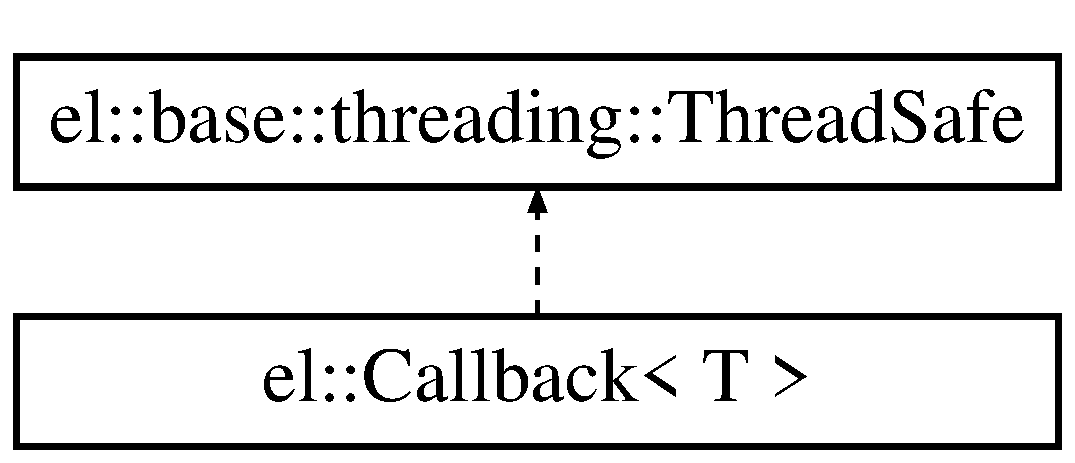
\includegraphics[height=2.000000cm]{classel_1_1Callback}
\end{center}
\end{figure}
\subsection*{Public Member Functions}
\begin{DoxyCompactItemize}
\item 
\hypertarget{classel_1_1Callback_a1e3089fd19a11965e7b98bd423116bbd}{bool {\bfseries enabled} (void) const }\label{classel_1_1Callback_a1e3089fd19a11965e7b98bd423116bbd}

\item 
\hypertarget{classel_1_1Callback_a05e68cb0b5ea4423913fa2ec4ea306b4}{void {\bfseries set\-Enabled} (bool enabled)}\label{classel_1_1Callback_a05e68cb0b5ea4423913fa2ec4ea306b4}

\end{DoxyCompactItemize}
\subsection*{Protected Member Functions}
\begin{DoxyCompactItemize}
\item 
\hypertarget{classel_1_1Callback_a8997c7971d65062c374ef24e653061be}{virtual void {\bfseries handle} (const T $\ast$handle\-Ptr)=0}\label{classel_1_1Callback_a8997c7971d65062c374ef24e653061be}

\end{DoxyCompactItemize}


The documentation for this class was generated from the following file\-:\begin{DoxyCompactItemize}
\item 
/users/disk9/cfse/\-Stage\-\_\-\-Malo/\-C\-P\-A\-C\-S\-Creator\-Lib/\-C\-P\-A\-C\-S\-Creator\-Lib/easylogging++.\-h\end{DoxyCompactItemize}

\hypertarget{classel_1_1base_1_1utils_1_1CommandLineArgs}{\section{el\-:\-:base\-:\-:utils\-:\-:Command\-Line\-Args Class Reference}
\label{classel_1_1base_1_1utils_1_1CommandLineArgs}\index{el\-::base\-::utils\-::\-Command\-Line\-Args@{el\-::base\-::utils\-::\-Command\-Line\-Args}}
}


Command line arguments for application if specified using \hyperlink{classel_1_1Helpers_a68748f618a0c2840b96dc12532b09bf0}{el\-::\-Helpers\-::set\-Args}(..) or S\-T\-A\-R\-T\-\_\-\-E\-A\-S\-Y\-L\-O\-G\-G\-I\-N\-G\-P\-P(..)  




{\ttfamily \#include $<$easylogging++.\-h$>$}

\subsection*{Public Member Functions}
\begin{DoxyCompactItemize}
\item 
\hypertarget{classel_1_1base_1_1utils_1_1CommandLineArgs_a9872b14450e9cd1c1bd96227743c083b}{{\bfseries Command\-Line\-Args} (int argc, const char $\ast$$\ast$argv)}\label{classel_1_1base_1_1utils_1_1CommandLineArgs_a9872b14450e9cd1c1bd96227743c083b}

\item 
\hypertarget{classel_1_1base_1_1utils_1_1CommandLineArgs_a297b31b31829d9545d6e808f4be9195c}{{\bfseries Command\-Line\-Args} (int argc, char $\ast$$\ast$argv)}\label{classel_1_1base_1_1utils_1_1CommandLineArgs_a297b31b31829d9545d6e808f4be9195c}

\item 
\hypertarget{classel_1_1base_1_1utils_1_1CommandLineArgs_a2d59b4184e0a6a314ef1c9a4c6d946e6}{void \hyperlink{classel_1_1base_1_1utils_1_1CommandLineArgs_a2d59b4184e0a6a314ef1c9a4c6d946e6}{set\-Args} (int argc, const char $\ast$$\ast$argv)}\label{classel_1_1base_1_1utils_1_1CommandLineArgs_a2d59b4184e0a6a314ef1c9a4c6d946e6}

\begin{DoxyCompactList}\small\item\em Sets arguments and parses them. \end{DoxyCompactList}\item 
\hypertarget{classel_1_1base_1_1utils_1_1CommandLineArgs_af88a16e6ce7b5d48f9679f304367b27a}{void \hyperlink{classel_1_1base_1_1utils_1_1CommandLineArgs_af88a16e6ce7b5d48f9679f304367b27a}{set\-Args} (int argc, char $\ast$$\ast$argv)}\label{classel_1_1base_1_1utils_1_1CommandLineArgs_af88a16e6ce7b5d48f9679f304367b27a}

\begin{DoxyCompactList}\small\item\em Sets arguments and parses them. \end{DoxyCompactList}\item 
\hypertarget{classel_1_1base_1_1utils_1_1CommandLineArgs_acc9fa8eeed2deecffb6019173de5ab48}{bool \hyperlink{classel_1_1base_1_1utils_1_1CommandLineArgs_acc9fa8eeed2deecffb6019173de5ab48}{has\-Param\-With\-Value} (const char $\ast$param\-Key) const }\label{classel_1_1base_1_1utils_1_1CommandLineArgs_acc9fa8eeed2deecffb6019173de5ab48}

\begin{DoxyCompactList}\small\item\em Returns true if arguments contain param\-Key with a value (seperated by '=') \end{DoxyCompactList}\item 
const char $\ast$ \hyperlink{classel_1_1base_1_1utils_1_1CommandLineArgs_ad1abe08dfdbdd95c72474197ba4a3cbd}{get\-Param\-Value} (const char $\ast$param\-Key) const 
\begin{DoxyCompactList}\small\item\em Returns value of arguments. \end{DoxyCompactList}\item 
\hypertarget{classel_1_1base_1_1utils_1_1CommandLineArgs_a83fbd7e5d8422e98a7d58d65283f144f}{bool \hyperlink{classel_1_1base_1_1utils_1_1CommandLineArgs_a83fbd7e5d8422e98a7d58d65283f144f}{has\-Param} (const char $\ast$param\-Key) const }\label{classel_1_1base_1_1utils_1_1CommandLineArgs_a83fbd7e5d8422e98a7d58d65283f144f}

\begin{DoxyCompactList}\small\item\em Return true if arguments has a param (not having a value) i,e without '='. \end{DoxyCompactList}\item 
\hypertarget{classel_1_1base_1_1utils_1_1CommandLineArgs_a014c586d14eb73f2ec1deb5b08bdd6a7}{bool \hyperlink{classel_1_1base_1_1utils_1_1CommandLineArgs_a014c586d14eb73f2ec1deb5b08bdd6a7}{empty} (void) const }\label{classel_1_1base_1_1utils_1_1CommandLineArgs_a014c586d14eb73f2ec1deb5b08bdd6a7}

\begin{DoxyCompactList}\small\item\em Returns true if no params available. This exclude argv\mbox{[}0\mbox{]}. \end{DoxyCompactList}\item 
\hypertarget{classel_1_1base_1_1utils_1_1CommandLineArgs_ab335b66a2ca2dea6c9c7b8d54760e975}{std\-::size\-\_\-t \hyperlink{classel_1_1base_1_1utils_1_1CommandLineArgs_ab335b66a2ca2dea6c9c7b8d54760e975}{size} (void) const }\label{classel_1_1base_1_1utils_1_1CommandLineArgs_ab335b66a2ca2dea6c9c7b8d54760e975}

\begin{DoxyCompactList}\small\item\em Returns total number of arguments. This exclude argv\mbox{[}0\mbox{]}. \end{DoxyCompactList}\end{DoxyCompactItemize}
\subsection*{Friends}
\begin{DoxyCompactItemize}
\item 
\hypertarget{classel_1_1base_1_1utils_1_1CommandLineArgs_aee5ba4c037136cd1d54026dd75927b10}{base\-::type\-::ostream\-\_\-t \& {\bfseries operator$<$$<$} (base\-::type\-::ostream\-\_\-t \&os, const \hyperlink{classel_1_1base_1_1utils_1_1CommandLineArgs}{Command\-Line\-Args} \&c)}\label{classel_1_1base_1_1utils_1_1CommandLineArgs_aee5ba4c037136cd1d54026dd75927b10}

\end{DoxyCompactItemize}


\subsection{Detailed Description}
Command line arguments for application if specified using \hyperlink{classel_1_1Helpers_a68748f618a0c2840b96dc12532b09bf0}{el\-::\-Helpers\-::set\-Args}(..) or S\-T\-A\-R\-T\-\_\-\-E\-A\-S\-Y\-L\-O\-G\-G\-I\-N\-G\-P\-P(..) 

\subsection{Member Function Documentation}
\hypertarget{classel_1_1base_1_1utils_1_1CommandLineArgs_ad1abe08dfdbdd95c72474197ba4a3cbd}{\index{el\-::base\-::utils\-::\-Command\-Line\-Args@{el\-::base\-::utils\-::\-Command\-Line\-Args}!get\-Param\-Value@{get\-Param\-Value}}
\index{get\-Param\-Value@{get\-Param\-Value}!el::base::utils::CommandLineArgs@{el\-::base\-::utils\-::\-Command\-Line\-Args}}
\subsubsection[{get\-Param\-Value}]{\setlength{\rightskip}{0pt plus 5cm}const char$\ast$ el\-::base\-::utils\-::\-Command\-Line\-Args\-::get\-Param\-Value (
\begin{DoxyParamCaption}
\item[{const char $\ast$}]{param\-Key}
\end{DoxyParamCaption}
) const}}\label{classel_1_1base_1_1utils_1_1CommandLineArgs_ad1abe08dfdbdd95c72474197ba4a3cbd}


Returns value of arguments. 

\begin{DoxySeeAlso}{See Also}
has\-Param\-With\-Value(const char$\ast$) 
\end{DoxySeeAlso}


The documentation for this class was generated from the following file\-:\begin{DoxyCompactItemize}
\item 
/users/disk9/cfse/\-Stage\-\_\-\-Malo/\-C\-P\-A\-C\-S\-Creator\-Lib/\-C\-P\-A\-C\-S\-Creator\-Lib/easylogging++.\-h\end{DoxyCompactItemize}

\hypertarget{classel_1_1Configuration}{\section{el\-:\-:Configuration Class Reference}
\label{classel_1_1Configuration}\index{el\-::\-Configuration@{el\-::\-Configuration}}
}


Represents single configuration that has representing level, configuration type and a string based value.  




{\ttfamily \#include $<$easylogging++.\-h$>$}

Inheritance diagram for el\-:\-:Configuration\-:\begin{figure}[H]
\begin{center}
\leavevmode
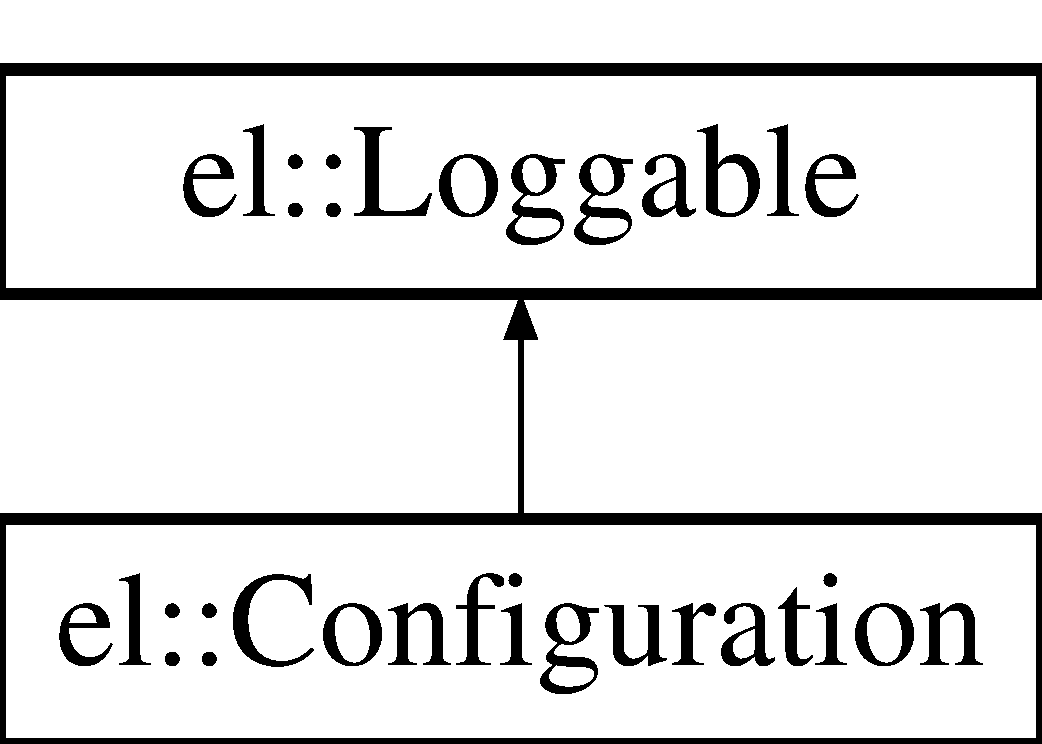
\includegraphics[height=2.000000cm]{classel_1_1Configuration}
\end{center}
\end{figure}
\subsection*{Classes}
\begin{DoxyCompactItemize}
\item 
class \hyperlink{classel_1_1Configuration_1_1Predicate}{Predicate}
\begin{DoxyCompactList}\small\item\em Used to find configuration from configuration (pointers) repository. Avoid using it. \end{DoxyCompactList}\end{DoxyCompactItemize}
\subsection*{Public Member Functions}
\begin{DoxyCompactItemize}
\item 
\hypertarget{classel_1_1Configuration_a71867a89e7d44cac62e0a436f01b484d}{{\bfseries Configuration} (const \hyperlink{classel_1_1Configuration}{Configuration} \&c)}\label{classel_1_1Configuration_a71867a89e7d44cac62e0a436f01b484d}

\item 
\hypertarget{classel_1_1Configuration_a80bc5b14f61906633cf695ea62e454a2}{\hyperlink{classel_1_1Configuration}{Configuration} \& {\bfseries operator=} (const \hyperlink{classel_1_1Configuration}{Configuration} \&c)}\label{classel_1_1Configuration_a80bc5b14f61906633cf695ea62e454a2}

\item 
\hypertarget{classel_1_1Configuration_a1a00abf955e028debaaf7556a647dbf5}{\hyperlink{classel_1_1Configuration_a1a00abf955e028debaaf7556a647dbf5}{Configuration} (\hyperlink{namespaceel_ab0ac6091262344c52dd2d3ad099e8e36}{Level} \hyperlink{classel_1_1Configuration_a66a96cf46d20204c50718f8a5e3622e2}{level}, \hyperlink{namespaceel_a281f5db6d6163678bc68a8b23b59e124}{Configuration\-Type} \hyperlink{classel_1_1Configuration_aab5091dcca176e309c0a2268ff55db0d}{configuration\-Type}, const std\-::string \&\hyperlink{classel_1_1Configuration_ab31605eb195a222cf32baa4922bb9a3c}{value})}\label{classel_1_1Configuration_a1a00abf955e028debaaf7556a647dbf5}

\begin{DoxyCompactList}\small\item\em Full constructor used to sets value of configuration. \end{DoxyCompactList}\item 
\hypertarget{classel_1_1Configuration_a66a96cf46d20204c50718f8a5e3622e2}{\hyperlink{namespaceel_ab0ac6091262344c52dd2d3ad099e8e36}{Level} \hyperlink{classel_1_1Configuration_a66a96cf46d20204c50718f8a5e3622e2}{level} (void) const }\label{classel_1_1Configuration_a66a96cf46d20204c50718f8a5e3622e2}

\begin{DoxyCompactList}\small\item\em Gets level of current configuration. \end{DoxyCompactList}\item 
\hypertarget{classel_1_1Configuration_aab5091dcca176e309c0a2268ff55db0d}{\hyperlink{namespaceel_a281f5db6d6163678bc68a8b23b59e124}{Configuration\-Type} \hyperlink{classel_1_1Configuration_aab5091dcca176e309c0a2268ff55db0d}{configuration\-Type} (void) const }\label{classel_1_1Configuration_aab5091dcca176e309c0a2268ff55db0d}

\begin{DoxyCompactList}\small\item\em Gets configuration type of current configuration. \end{DoxyCompactList}\item 
\hypertarget{classel_1_1Configuration_ab31605eb195a222cf32baa4922bb9a3c}{const std\-::string \& \hyperlink{classel_1_1Configuration_ab31605eb195a222cf32baa4922bb9a3c}{value} (void) const }\label{classel_1_1Configuration_ab31605eb195a222cf32baa4922bb9a3c}

\begin{DoxyCompactList}\small\item\em Gets string based configuration value. \end{DoxyCompactList}\item 
void \hyperlink{classel_1_1Configuration_a04755de11422d7570869433ea157b705}{set\-Value} (const std\-::string \&\hyperlink{classel_1_1Configuration_ab31605eb195a222cf32baa4922bb9a3c}{value})
\begin{DoxyCompactList}\small\item\em Set string based configuration value. \end{DoxyCompactList}\item 
\hypertarget{classel_1_1Configuration_a82c87e1a93211a1d21da99570f47dd49}{virtual void {\bfseries log} (el\-::base\-::type\-::ostream\-\_\-t \&os) const }\label{classel_1_1Configuration_a82c87e1a93211a1d21da99570f47dd49}

\end{DoxyCompactItemize}


\subsection{Detailed Description}
Represents single configuration that has representing level, configuration type and a string based value. 

String based value means any value either its boolean, integer or string itself, it will be embedded inside quotes and will be parsed later.

Consider some examples below\-:
\begin{DoxyItemize}
\item \hyperlink{classel_1_1Configuration}{el\-::\-Configuration} conf\-Enabled\-Info(\hyperlink{namespaceel_ab0ac6091262344c52dd2d3ad099e8e36a4059b0251f66a18cb56f544728796875}{el\-::\-Level\-::\-Info}, \hyperlink{namespaceel_a281f5db6d6163678bc68a8b23b59e124a00d23a76e43b46dae9ec7aa9dcbebb32}{el\-::\-Configuration\-Type\-::\-Enabled}, \char`\"{}true\char`\"{});
\item \hyperlink{classel_1_1Configuration}{el\-::\-Configuration} conf\-Max\-Log\-File\-Size\-Info(\hyperlink{namespaceel_ab0ac6091262344c52dd2d3ad099e8e36a4059b0251f66a18cb56f544728796875}{el\-::\-Level\-::\-Info}, \hyperlink{namespaceel_a281f5db6d6163678bc68a8b23b59e124a4b35e615142d60db6383426f051e700b}{el\-::\-Configuration\-Type\-::\-Max\-Log\-File\-Size}, \char`\"{}2048\char`\"{});
\item \hyperlink{classel_1_1Configuration}{el\-::\-Configuration} conf\-Filename\-Info(\hyperlink{namespaceel_ab0ac6091262344c52dd2d3ad099e8e36a4059b0251f66a18cb56f544728796875}{el\-::\-Level\-::\-Info}, \hyperlink{namespaceel_a281f5db6d6163678bc68a8b23b59e124a1351017ac6423911223bc19a8cb7c653}{el\-::\-Configuration\-Type\-::\-Filename}, \char`\"{}/var/log/my.\-log\char`\"{}); 
\end{DoxyItemize}

\subsection{Member Function Documentation}
\hypertarget{classel_1_1Configuration_a04755de11422d7570869433ea157b705}{\index{el\-::\-Configuration@{el\-::\-Configuration}!set\-Value@{set\-Value}}
\index{set\-Value@{set\-Value}!el::Configuration@{el\-::\-Configuration}}
\subsubsection[{set\-Value}]{\setlength{\rightskip}{0pt plus 5cm}void el\-::\-Configuration\-::set\-Value (
\begin{DoxyParamCaption}
\item[{const std\-::string \&}]{value}
\end{DoxyParamCaption}
)\hspace{0.3cm}{\ttfamily [inline]}}}\label{classel_1_1Configuration_a04755de11422d7570869433ea157b705}


Set string based configuration value. 


\begin{DoxyParams}{Parameters}
{\em value} & Value to set. Values have to be std\-::string; For boolean values use \char`\"{}true\char`\"{}, \char`\"{}false\char`\"{}, for any integral values use them in quotes. They will be parsed when configuring \\
\hline
\end{DoxyParams}


The documentation for this class was generated from the following file\-:\begin{DoxyCompactItemize}
\item 
/users/disk9/cfse/\-Stage\-\_\-\-Malo/\-C\-P\-A\-C\-S\-Creator\-Lib/\-C\-P\-A\-C\-S\-Creator\-Lib/easylogging++.\-h\end{DoxyCompactItemize}

\hypertarget{classel_1_1Configurations}{\section{el\-:\-:Configurations Class Reference}
\label{classel_1_1Configurations}\index{el\-::\-Configurations@{el\-::\-Configurations}}
}


Thread-\/safe \hyperlink{classel_1_1Configuration}{Configuration} repository.  




{\ttfamily \#include $<$easylogging++.\-h$>$}

Inheritance diagram for el\-:\-:Configurations\-:\begin{figure}[H]
\begin{center}
\leavevmode
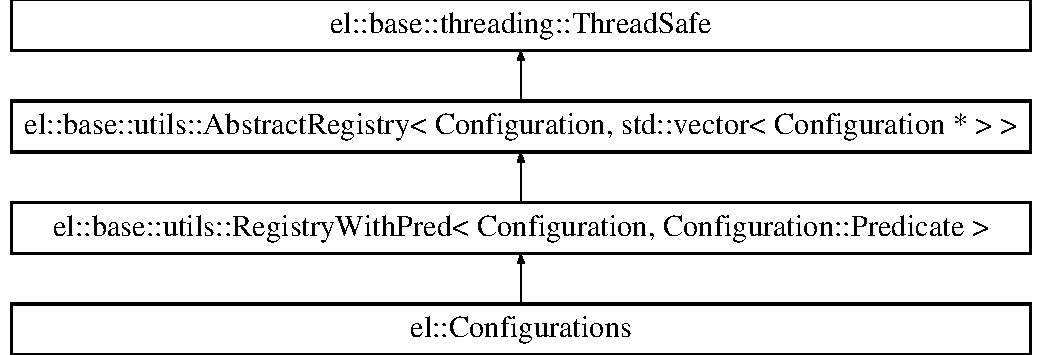
\includegraphics[height=4.000000cm]{classel_1_1Configurations}
\end{center}
\end{figure}
\subsection*{Classes}
\begin{DoxyCompactItemize}
\item 
class \hyperlink{classel_1_1Configurations_1_1Parser}{Parser}
\begin{DoxyCompactList}\small\item\em \hyperlink{classel_1_1Configurations_1_1Parser}{Parser} used internally to parse configurations from file or text. \end{DoxyCompactList}\end{DoxyCompactItemize}
\subsection*{Public Member Functions}
\begin{DoxyCompactItemize}
\item 
\hypertarget{classel_1_1Configurations_ae299dd1b60a1df9c013cc23029242a77}{\hyperlink{classel_1_1Configurations_ae299dd1b60a1df9c013cc23029242a77}{Configurations} (void)}\label{classel_1_1Configurations_ae299dd1b60a1df9c013cc23029242a77}

\begin{DoxyCompactList}\small\item\em Default constructor with empty repository. \end{DoxyCompactList}\item 
\hyperlink{classel_1_1Configurations_ae341bd647734d1180a5a138222d2f1ea}{Configurations} (const std\-::string \&\hyperlink{classel_1_1Configurations_a18df64bb5cd97bee672160290133141c}{configuration\-File}, bool use\-Defaults\-For\-Remaining=true, \hyperlink{classel_1_1Configurations}{Configurations} $\ast$base=nullptr)
\begin{DoxyCompactList}\small\item\em Constructor used to set configurations using configuration file. \end{DoxyCompactList}\item 
bool \hyperlink{classel_1_1Configurations_aaa098126d64a5ee04a3944b1a65dcdca}{parse\-From\-File} (const std\-::string \&\hyperlink{classel_1_1Configurations_a18df64bb5cd97bee672160290133141c}{configuration\-File}, \hyperlink{classel_1_1Configurations}{Configurations} $\ast$base=nullptr)
\begin{DoxyCompactList}\small\item\em Parses configuration from file. \end{DoxyCompactList}\item 
bool \hyperlink{classel_1_1Configurations_af262a41dff665a11889261137b62af4a}{parse\-From\-Text} (const std\-::string \&configurations\-String, \hyperlink{classel_1_1Configurations}{Configurations} $\ast$base=nullptr)
\begin{DoxyCompactList}\small\item\em Parse configurations from configuration string. \end{DoxyCompactList}\item 
void \hyperlink{classel_1_1Configurations_a4c6db218908b39d23cc09b1a16a18e83}{set\-From\-Base} (\hyperlink{classel_1_1Configurations}{Configurations} $\ast$base)
\begin{DoxyCompactList}\small\item\em Sets configuration based-\/off an existing configurations. \end{DoxyCompactList}\item 
bool \hyperlink{classel_1_1Configurations_a1e812370f896b6429bf46b31fcd4e3e0}{has\-Configuration} (\hyperlink{namespaceel_a281f5db6d6163678bc68a8b23b59e124}{Configuration\-Type} configuration\-Type)
\begin{DoxyCompactList}\small\item\em Determines whether or not specified configuration type exists in the repository. \end{DoxyCompactList}\item 
bool \hyperlink{classel_1_1Configurations_a5313557efac3b0c78f973a5a1d685277}{has\-Configuration} (\hyperlink{namespaceel_ab0ac6091262344c52dd2d3ad099e8e36}{Level} level, \hyperlink{namespaceel_a281f5db6d6163678bc68a8b23b59e124}{Configuration\-Type} configuration\-Type)
\begin{DoxyCompactList}\small\item\em Determines whether or not specified configuration type exists for specified level. \end{DoxyCompactList}\item 
void \hyperlink{classel_1_1Configurations_a332717de96efc851a202b7afcc5e395c}{set} (\hyperlink{namespaceel_ab0ac6091262344c52dd2d3ad099e8e36}{Level} level, \hyperlink{namespaceel_a281f5db6d6163678bc68a8b23b59e124}{Configuration\-Type} configuration\-Type, const std\-::string \&value)
\begin{DoxyCompactList}\small\item\em Sets value of configuration for specified level. \end{DoxyCompactList}\item 
void \hyperlink{classel_1_1Configurations_a0ab07520b9409fe9f2c16a705d6936f1}{set} (\hyperlink{classel_1_1Configuration}{Configuration} $\ast$conf)
\begin{DoxyCompactList}\small\item\em Sets single configuration based on other single configuration. \end{DoxyCompactList}\item 
\hypertarget{classel_1_1Configurations_a6da4bc9bd6a14dc44feaf25163e998ca}{\hyperlink{classel_1_1Configuration}{Configuration} $\ast$ {\bfseries get} (\hyperlink{namespaceel_ab0ac6091262344c52dd2d3ad099e8e36}{Level} level, \hyperlink{namespaceel_a281f5db6d6163678bc68a8b23b59e124}{Configuration\-Type} configuration\-Type)}\label{classel_1_1Configurations_a6da4bc9bd6a14dc44feaf25163e998ca}

\item 
void \hyperlink{classel_1_1Configurations_a56c82c15ea39cc230a5c85ec2c41cbfd}{set\-Globally} (\hyperlink{namespaceel_a281f5db6d6163678bc68a8b23b59e124}{Configuration\-Type} configuration\-Type, const std\-::string \&value)
\begin{DoxyCompactList}\small\item\em Sets configuration for all levels. \end{DoxyCompactList}\item 
\hypertarget{classel_1_1Configurations_a2a13be6154439286a68d2eccf8417edf}{void \hyperlink{classel_1_1Configurations_a2a13be6154439286a68d2eccf8417edf}{clear} (void)}\label{classel_1_1Configurations_a2a13be6154439286a68d2eccf8417edf}

\begin{DoxyCompactList}\small\item\em Clears repository so that all the configurations are unset. \end{DoxyCompactList}\item 
const std\-::string \& \hyperlink{classel_1_1Configurations_a18df64bb5cd97bee672160290133141c}{configuration\-File} (void) const 
\begin{DoxyCompactList}\small\item\em Gets configuration file used in parsing this configurations. \end{DoxyCompactList}\item 
\hypertarget{classel_1_1Configurations_ab34fa2ed4ac77f47b41e464c2d186239}{void \hyperlink{classel_1_1Configurations_ab34fa2ed4ac77f47b41e464c2d186239}{set\-To\-Default} (void)}\label{classel_1_1Configurations_ab34fa2ed4ac77f47b41e464c2d186239}

\begin{DoxyCompactList}\small\item\em Sets configurations to \char`\"{}factory based\char`\"{} configurations. \end{DoxyCompactList}\item 
void \hyperlink{classel_1_1Configurations_ad89b7d2dd750e4d1b3deff800e278fdb}{set\-Remaining\-To\-Default} (void)
\begin{DoxyCompactList}\small\item\em Lets you set the remaining configurations to default. \end{DoxyCompactList}\end{DoxyCompactItemize}
\subsection*{Friends}
\begin{DoxyCompactItemize}
\item 
\hypertarget{classel_1_1Configurations_a6efe246b312d02731fb0e1d120c0331d}{class {\bfseries el\-::\-Loggers}}\label{classel_1_1Configurations_a6efe246b312d02731fb0e1d120c0331d}

\end{DoxyCompactItemize}
\subsection*{Additional Inherited Members}


\subsection{Detailed Description}
Thread-\/safe \hyperlink{classel_1_1Configuration}{Configuration} repository. 

This repository represents configurations for all the levels and configuration type mapped to a value. 

\subsection{Constructor \& Destructor Documentation}
\hypertarget{classel_1_1Configurations_ae341bd647734d1180a5a138222d2f1ea}{\index{el\-::\-Configurations@{el\-::\-Configurations}!Configurations@{Configurations}}
\index{Configurations@{Configurations}!el::Configurations@{el\-::\-Configurations}}
\subsubsection[{Configurations}]{\setlength{\rightskip}{0pt plus 5cm}el\-::\-Configurations\-::\-Configurations (
\begin{DoxyParamCaption}
\item[{const std\-::string \&}]{configuration\-File, }
\item[{bool}]{use\-Defaults\-For\-Remaining = {\ttfamily true}, }
\item[{{\bf Configurations} $\ast$}]{base = {\ttfamily nullptr}}
\end{DoxyParamCaption}
)}}\label{classel_1_1Configurations_ae341bd647734d1180a5a138222d2f1ea}


Constructor used to set configurations using configuration file. 


\begin{DoxyParams}{Parameters}
{\em configuration\-File} & Full path to configuration file \\
\hline
{\em use\-Defaults\-For\-Remaining} & Lets you set the remaining configurations to default. \\
\hline
{\em base} & If provided, this configuration will be based off existing repository that this argument is pointing to. \\
\hline
\end{DoxyParams}
\begin{DoxySeeAlso}{See Also}
\hyperlink{classel_1_1Configurations_aaa098126d64a5ee04a3944b1a65dcdca}{parse\-From\-File(const std\-::string\&, Configurations$\ast$ base)} 

\hyperlink{classel_1_1Configurations_ad89b7d2dd750e4d1b3deff800e278fdb}{set\-Remaining\-To\-Default()} 
\end{DoxySeeAlso}


\subsection{Member Function Documentation}
\hypertarget{classel_1_1Configurations_a18df64bb5cd97bee672160290133141c}{\index{el\-::\-Configurations@{el\-::\-Configurations}!configuration\-File@{configuration\-File}}
\index{configuration\-File@{configuration\-File}!el::Configurations@{el\-::\-Configurations}}
\subsubsection[{configuration\-File}]{\setlength{\rightskip}{0pt plus 5cm}const std\-::string\& el\-::\-Configurations\-::configuration\-File (
\begin{DoxyParamCaption}
\item[{void}]{}
\end{DoxyParamCaption}
) const\hspace{0.3cm}{\ttfamily [inline]}}}\label{classel_1_1Configurations_a18df64bb5cd97bee672160290133141c}


Gets configuration file used in parsing this configurations. 

If this repository was set manually or by text this returns empty string. \hypertarget{classel_1_1Configurations_a1e812370f896b6429bf46b31fcd4e3e0}{\index{el\-::\-Configurations@{el\-::\-Configurations}!has\-Configuration@{has\-Configuration}}
\index{has\-Configuration@{has\-Configuration}!el::Configurations@{el\-::\-Configurations}}
\subsubsection[{has\-Configuration}]{\setlength{\rightskip}{0pt plus 5cm}bool el\-::\-Configurations\-::has\-Configuration (
\begin{DoxyParamCaption}
\item[{{\bf Configuration\-Type}}]{configuration\-Type}
\end{DoxyParamCaption}
)}}\label{classel_1_1Configurations_a1e812370f896b6429bf46b31fcd4e3e0}


Determines whether or not specified configuration type exists in the repository. 

Returns as soon as first level is found. 
\begin{DoxyParams}{Parameters}
{\em configuration\-Type} & Type of configuration to check existence for. \\
\hline
\end{DoxyParams}
\hypertarget{classel_1_1Configurations_a5313557efac3b0c78f973a5a1d685277}{\index{el\-::\-Configurations@{el\-::\-Configurations}!has\-Configuration@{has\-Configuration}}
\index{has\-Configuration@{has\-Configuration}!el::Configurations@{el\-::\-Configurations}}
\subsubsection[{has\-Configuration}]{\setlength{\rightskip}{0pt plus 5cm}bool el\-::\-Configurations\-::has\-Configuration (
\begin{DoxyParamCaption}
\item[{{\bf Level}}]{level, }
\item[{{\bf Configuration\-Type}}]{configuration\-Type}
\end{DoxyParamCaption}
)}}\label{classel_1_1Configurations_a5313557efac3b0c78f973a5a1d685277}


Determines whether or not specified configuration type exists for specified level. 


\begin{DoxyParams}{Parameters}
{\em level} & Level to check \\
\hline
{\em configuration\-Type} & Type of configuration to check existence for. \\
\hline
\end{DoxyParams}
\hypertarget{classel_1_1Configurations_aaa098126d64a5ee04a3944b1a65dcdca}{\index{el\-::\-Configurations@{el\-::\-Configurations}!parse\-From\-File@{parse\-From\-File}}
\index{parse\-From\-File@{parse\-From\-File}!el::Configurations@{el\-::\-Configurations}}
\subsubsection[{parse\-From\-File}]{\setlength{\rightskip}{0pt plus 5cm}bool el\-::\-Configurations\-::parse\-From\-File (
\begin{DoxyParamCaption}
\item[{const std\-::string \&}]{configuration\-File, }
\item[{{\bf Configurations} $\ast$}]{base = {\ttfamily nullptr}}
\end{DoxyParamCaption}
)}}\label{classel_1_1Configurations_aaa098126d64a5ee04a3944b1a65dcdca}


Parses configuration from file. 


\begin{DoxyParams}{Parameters}
{\em configuration\-File} & Full path to configuration file \\
\hline
{\em base} & \hyperlink{classel_1_1Configurations}{Configurations} to base new configuration repository off. This value is used when you want to use existing \hyperlink{classel_1_1Configurations}{Configurations} to base all the values and then set rest of configuration via configuration file. \\
\hline
\end{DoxyParams}
\begin{DoxyReturn}{Returns}
True if successfully parsed, false otherwise. You may define 'E\-L\-P\-P\-\_\-\-D\-E\-B\-U\-G\-\_\-\-A\-S\-S\-E\-R\-T\-\_\-\-F\-A\-I\-L\-U\-R\-E' to make sure you do not proceed without successful parse. 
\end{DoxyReturn}
\hypertarget{classel_1_1Configurations_af262a41dff665a11889261137b62af4a}{\index{el\-::\-Configurations@{el\-::\-Configurations}!parse\-From\-Text@{parse\-From\-Text}}
\index{parse\-From\-Text@{parse\-From\-Text}!el::Configurations@{el\-::\-Configurations}}
\subsubsection[{parse\-From\-Text}]{\setlength{\rightskip}{0pt plus 5cm}bool el\-::\-Configurations\-::parse\-From\-Text (
\begin{DoxyParamCaption}
\item[{const std\-::string \&}]{configurations\-String, }
\item[{{\bf Configurations} $\ast$}]{base = {\ttfamily nullptr}}
\end{DoxyParamCaption}
)}}\label{classel_1_1Configurations_af262a41dff665a11889261137b62af4a}


Parse configurations from configuration string. 

This configuration string has same syntax as configuration file contents. Make sure all the necessary new line characters are provided. 
\begin{DoxyParams}{Parameters}
{\em base} & \hyperlink{classel_1_1Configurations}{Configurations} to base new configuration repository off. This value is used when you want to use existing \hyperlink{classel_1_1Configurations}{Configurations} to base all the values and then set rest of configuration via configuration text. \\
\hline
\end{DoxyParams}
\begin{DoxyReturn}{Returns}
True if successfully parsed, false otherwise. You may define 'E\-L\-P\-P\-\_\-\-D\-E\-B\-U\-G\-\_\-\-A\-S\-S\-E\-R\-T\-\_\-\-F\-A\-I\-L\-U\-R\-E' to make sure you do not proceed without successful parse. 
\end{DoxyReturn}
\hypertarget{classel_1_1Configurations_a332717de96efc851a202b7afcc5e395c}{\index{el\-::\-Configurations@{el\-::\-Configurations}!set@{set}}
\index{set@{set}!el::Configurations@{el\-::\-Configurations}}
\subsubsection[{set}]{\setlength{\rightskip}{0pt plus 5cm}void el\-::\-Configurations\-::set (
\begin{DoxyParamCaption}
\item[{{\bf Level}}]{level, }
\item[{{\bf Configuration\-Type}}]{configuration\-Type, }
\item[{const std\-::string \&}]{value}
\end{DoxyParamCaption}
)}}\label{classel_1_1Configurations_a332717de96efc851a202b7afcc5e395c}


Sets value of configuration for specified level. 

Any existing configuration for specified level will be replaced. Also note that configuration types \hyperlink{namespaceel_a281f5db6d6163678bc68a8b23b59e124a945b6ef21f66457079a6ab7b6c3459f9}{Configuration\-Type\-::\-Subsecond\-Precision} and \hyperlink{namespaceel_a281f5db6d6163678bc68a8b23b59e124abe9e43d200c5698cb8519daed7035874}{Configuration\-Type\-::\-Performance\-Tracking} will be ignored if not set for \hyperlink{namespaceel_ab0ac6091262344c52dd2d3ad099e8e36a4cc6684df7b4a92b1dec6fce3264fac8}{Level\-::\-Global} because these configurations are not dependant on level. 
\begin{DoxyParams}{Parameters}
{\em level} & Level to set configuration for (\hyperlink{namespaceel_ab0ac6091262344c52dd2d3ad099e8e36}{el\-::\-Level}). \\
\hline
{\em configuration\-Type} & Type of configuration (\hyperlink{namespaceel_a281f5db6d6163678bc68a8b23b59e124}{el\-::\-Configuration\-Type}) \\
\hline
{\em value} & A string based value. Regardless of what the data type of configuration is, it will always be string from users' point of view. This is then parsed later to be used internally. \\
\hline
\end{DoxyParams}
\begin{DoxySeeAlso}{See Also}
\hyperlink{classel_1_1Configuration_a04755de11422d7570869433ea157b705}{Configuration\-::set\-Value(const std\-::string\& value)} 

\hyperlink{namespaceel_ab0ac6091262344c52dd2d3ad099e8e36}{el\-::\-Level} 

\hyperlink{namespaceel_a281f5db6d6163678bc68a8b23b59e124}{el\-::\-Configuration\-Type} 
\end{DoxySeeAlso}
\hypertarget{classel_1_1Configurations_a0ab07520b9409fe9f2c16a705d6936f1}{\index{el\-::\-Configurations@{el\-::\-Configurations}!set@{set}}
\index{set@{set}!el::Configurations@{el\-::\-Configurations}}
\subsubsection[{set}]{\setlength{\rightskip}{0pt plus 5cm}void el\-::\-Configurations\-::set (
\begin{DoxyParamCaption}
\item[{{\bf Configuration} $\ast$}]{conf}
\end{DoxyParamCaption}
)}}\label{classel_1_1Configurations_a0ab07520b9409fe9f2c16a705d6936f1}


Sets single configuration based on other single configuration. 

\begin{DoxySeeAlso}{See Also}
\hyperlink{classel_1_1Configurations_a332717de96efc851a202b7afcc5e395c}{set(\-Level level, Configuration\-Type configuration\-Type, const std\-::string\& value)} 
\end{DoxySeeAlso}
\hypertarget{classel_1_1Configurations_a4c6db218908b39d23cc09b1a16a18e83}{\index{el\-::\-Configurations@{el\-::\-Configurations}!set\-From\-Base@{set\-From\-Base}}
\index{set\-From\-Base@{set\-From\-Base}!el::Configurations@{el\-::\-Configurations}}
\subsubsection[{set\-From\-Base}]{\setlength{\rightskip}{0pt plus 5cm}void el\-::\-Configurations\-::set\-From\-Base (
\begin{DoxyParamCaption}
\item[{{\bf Configurations} $\ast$}]{base}
\end{DoxyParamCaption}
)}}\label{classel_1_1Configurations_a4c6db218908b39d23cc09b1a16a18e83}


Sets configuration based-\/off an existing configurations. 


\begin{DoxyParams}{Parameters}
{\em base} & Pointer to existing configurations. \\
\hline
\end{DoxyParams}
\hypertarget{classel_1_1Configurations_a56c82c15ea39cc230a5c85ec2c41cbfd}{\index{el\-::\-Configurations@{el\-::\-Configurations}!set\-Globally@{set\-Globally}}
\index{set\-Globally@{set\-Globally}!el::Configurations@{el\-::\-Configurations}}
\subsubsection[{set\-Globally}]{\setlength{\rightskip}{0pt plus 5cm}void el\-::\-Configurations\-::set\-Globally (
\begin{DoxyParamCaption}
\item[{{\bf Configuration\-Type}}]{configuration\-Type, }
\item[{const std\-::string \&}]{value}
\end{DoxyParamCaption}
)\hspace{0.3cm}{\ttfamily [inline]}}}\label{classel_1_1Configurations_a56c82c15ea39cc230a5c85ec2c41cbfd}


Sets configuration for all levels. 


\begin{DoxyParams}{Parameters}
{\em configuration\-Type} & Type of configuration \\
\hline
{\em value} & String based value \\
\hline
\end{DoxyParams}
\begin{DoxySeeAlso}{See Also}
\hyperlink{classel_1_1Configurations_a332717de96efc851a202b7afcc5e395c}{Configurations\-::set(\-Level level, Configuration\-Type configuration\-Type, const std\-::string\& value)} 
\end{DoxySeeAlso}
\hypertarget{classel_1_1Configurations_ad89b7d2dd750e4d1b3deff800e278fdb}{\index{el\-::\-Configurations@{el\-::\-Configurations}!set\-Remaining\-To\-Default@{set\-Remaining\-To\-Default}}
\index{set\-Remaining\-To\-Default@{set\-Remaining\-To\-Default}!el::Configurations@{el\-::\-Configurations}}
\subsubsection[{set\-Remaining\-To\-Default}]{\setlength{\rightskip}{0pt plus 5cm}void el\-::\-Configurations\-::set\-Remaining\-To\-Default (
\begin{DoxyParamCaption}
\item[{void}]{}
\end{DoxyParamCaption}
)}}\label{classel_1_1Configurations_ad89b7d2dd750e4d1b3deff800e278fdb}


Lets you set the remaining configurations to default. 

By remaining, it means that the level/type a configuration does not exist for. This function is useful when you want to minimize chances of failures, e.\-g, if you have a configuration file that sets configuration for all the configurations except for Enabled or not, we use this so that E\-N\-A\-B\-L\-E\-D is set to default i.\-e, true. If you dont do this explicitly (either by calling this function or by using second param in Constructor and try to access a value, an error is thrown 

The documentation for this class was generated from the following file\-:\begin{DoxyCompactItemize}
\item 
/users/disk9/cfse/\-Stage\-\_\-\-Malo/\-C\-P\-A\-C\-S\-Creator\-Lib/\-C\-P\-A\-C\-S\-Creator\-Lib/easylogging++.\-h\end{DoxyCompactItemize}

\hypertarget{classel_1_1ConfigurationTypeHelper}{\section{el\-:\-:Configuration\-Type\-Helper Class Reference}
\label{classel_1_1ConfigurationTypeHelper}\index{el\-::\-Configuration\-Type\-Helper@{el\-::\-Configuration\-Type\-Helper}}
}


Static class that contains helper functions for \hyperlink{namespaceel_a281f5db6d6163678bc68a8b23b59e124}{el\-::\-Configuration\-Type}.  




{\ttfamily \#include $<$easylogging++.\-h$>$}

Inheritance diagram for el\-:\-:Configuration\-Type\-Helper\-:\begin{figure}[H]
\begin{center}
\leavevmode
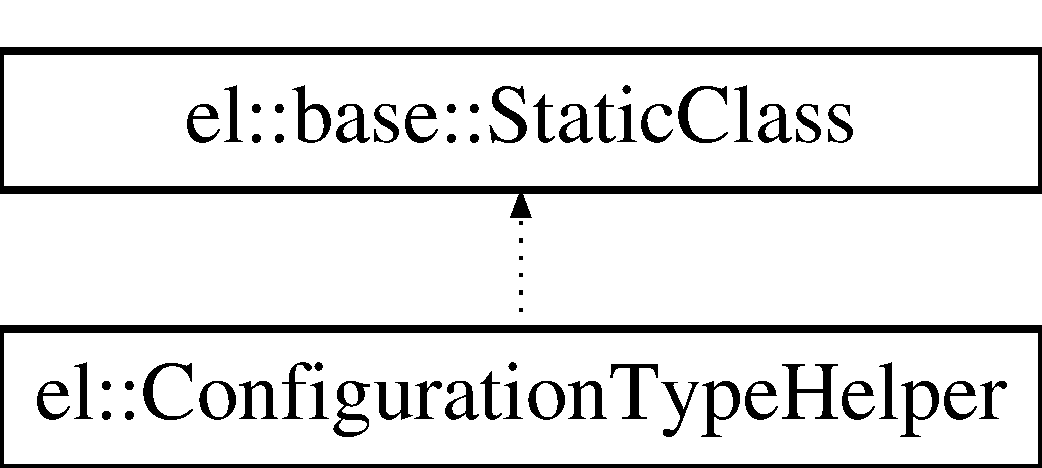
\includegraphics[height=2.000000cm]{classel_1_1ConfigurationTypeHelper}
\end{center}
\end{figure}
\subsection*{Static Public Member Functions}
\begin{DoxyCompactItemize}
\item 
\hypertarget{classel_1_1ConfigurationTypeHelper_aa53161071fee3ce3f371ab90c62d5fc2}{static base\-::type\-::\-Enum\-Type \hyperlink{classel_1_1ConfigurationTypeHelper_aa53161071fee3ce3f371ab90c62d5fc2}{cast\-To\-Int} (\hyperlink{namespaceel_a281f5db6d6163678bc68a8b23b59e124}{Configuration\-Type} configuration\-Type)}\label{classel_1_1ConfigurationTypeHelper_aa53161071fee3ce3f371ab90c62d5fc2}

\begin{DoxyCompactList}\small\item\em Casts configuration type to int, useful for iterating through enum. \end{DoxyCompactList}\item 
\hypertarget{classel_1_1ConfigurationTypeHelper_a62301cbc966cf7e7e2a7b55cc3259996}{static \hyperlink{namespaceel_a281f5db6d6163678bc68a8b23b59e124}{Configuration\-Type} \hyperlink{classel_1_1ConfigurationTypeHelper_a62301cbc966cf7e7e2a7b55cc3259996}{cast\-From\-Int} (base\-::type\-::\-Enum\-Type c)}\label{classel_1_1ConfigurationTypeHelper_a62301cbc966cf7e7e2a7b55cc3259996}

\begin{DoxyCompactList}\small\item\em Casts int(ushort) to configurationt type, useful for iterating through enum. \end{DoxyCompactList}\item 
static const char $\ast$ \hyperlink{classel_1_1ConfigurationTypeHelper_ad7f0a19c416c4a8ddaf85330b141383c}{convert\-To\-String} (\hyperlink{namespaceel_a281f5db6d6163678bc68a8b23b59e124}{Configuration\-Type} configuration\-Type)
\begin{DoxyCompactList}\small\item\em Converts configuration type to associated const char$\ast$. \end{DoxyCompactList}\item 
static \hyperlink{namespaceel_a281f5db6d6163678bc68a8b23b59e124}{Configuration\-Type} \hyperlink{classel_1_1ConfigurationTypeHelper_af4a35305e3941fd578e55fec624eba43}{convert\-From\-String} (const char $\ast$config\-Str)
\begin{DoxyCompactList}\small\item\em Converts from config\-Str to Configuration\-Type. \end{DoxyCompactList}\item 
static void \hyperlink{classel_1_1ConfigurationTypeHelper_aa0524147f792309fc09e0b8d14826c17}{for\-Each\-Config\-Type} (base\-::type\-::\-Enum\-Type $\ast$start\-Index, const std\-::function$<$ bool(void)$>$ \&fn)
\begin{DoxyCompactList}\small\item\em Applies specified function to each configuration type starting from start\-Index. \end{DoxyCompactList}\end{DoxyCompactItemize}
\subsection*{Static Public Attributes}
\begin{DoxyCompactItemize}
\item 
\hypertarget{classel_1_1ConfigurationTypeHelper_ab7266e698eb32dec2da285325a66e322}{static const base\-::type\-::\-Enum\-Type \hyperlink{classel_1_1ConfigurationTypeHelper_ab7266e698eb32dec2da285325a66e322}{k\-Min\-Valid} = static\-\_\-cast$<$base\-::type\-::\-Enum\-Type$>$(\hyperlink{namespaceel_a281f5db6d6163678bc68a8b23b59e124a00d23a76e43b46dae9ec7aa9dcbebb32}{Configuration\-Type\-::\-Enabled})}\label{classel_1_1ConfigurationTypeHelper_ab7266e698eb32dec2da285325a66e322}

\begin{DoxyCompactList}\small\item\em Represents minimum valid configuration type. Useful when iterating through enum. \end{DoxyCompactList}\item 
\hypertarget{classel_1_1ConfigurationTypeHelper_aa02f3cefb127e7eb97d7e1dd7f51a12d}{static const base\-::type\-::\-Enum\-Type \hyperlink{classel_1_1ConfigurationTypeHelper_aa02f3cefb127e7eb97d7e1dd7f51a12d}{k\-Max\-Valid} = static\-\_\-cast$<$base\-::type\-::\-Enum\-Type$>$(\hyperlink{namespaceel_a281f5db6d6163678bc68a8b23b59e124a4b35e615142d60db6383426f051e700b}{Configuration\-Type\-::\-Max\-Log\-File\-Size})}\label{classel_1_1ConfigurationTypeHelper_aa02f3cefb127e7eb97d7e1dd7f51a12d}

\begin{DoxyCompactList}\small\item\em Represents maximum valid configuration type. This is used internally and you should not need it. \end{DoxyCompactList}\end{DoxyCompactItemize}


\subsection{Detailed Description}
Static class that contains helper functions for \hyperlink{namespaceel_a281f5db6d6163678bc68a8b23b59e124}{el\-::\-Configuration\-Type}. 

\subsection{Member Function Documentation}
\hypertarget{classel_1_1ConfigurationTypeHelper_af4a35305e3941fd578e55fec624eba43}{\index{el\-::\-Configuration\-Type\-Helper@{el\-::\-Configuration\-Type\-Helper}!convert\-From\-String@{convert\-From\-String}}
\index{convert\-From\-String@{convert\-From\-String}!el::ConfigurationTypeHelper@{el\-::\-Configuration\-Type\-Helper}}
\subsubsection[{convert\-From\-String}]{\setlength{\rightskip}{0pt plus 5cm}static {\bf Configuration\-Type} el\-::\-Configuration\-Type\-Helper\-::convert\-From\-String (
\begin{DoxyParamCaption}
\item[{const char $\ast$}]{config\-Str}
\end{DoxyParamCaption}
)\hspace{0.3cm}{\ttfamily [static]}}}\label{classel_1_1ConfigurationTypeHelper_af4a35305e3941fd578e55fec624eba43}


Converts from config\-Str to Configuration\-Type. 


\begin{DoxyParams}{Parameters}
{\em config\-Str} & Upper case string based configuration type. Lower case is also valid but providing upper case is recommended. \\
\hline
\end{DoxyParams}
\hypertarget{classel_1_1ConfigurationTypeHelper_ad7f0a19c416c4a8ddaf85330b141383c}{\index{el\-::\-Configuration\-Type\-Helper@{el\-::\-Configuration\-Type\-Helper}!convert\-To\-String@{convert\-To\-String}}
\index{convert\-To\-String@{convert\-To\-String}!el::ConfigurationTypeHelper@{el\-::\-Configuration\-Type\-Helper}}
\subsubsection[{convert\-To\-String}]{\setlength{\rightskip}{0pt plus 5cm}static const char$\ast$ el\-::\-Configuration\-Type\-Helper\-::convert\-To\-String (
\begin{DoxyParamCaption}
\item[{{\bf Configuration\-Type}}]{configuration\-Type}
\end{DoxyParamCaption}
)\hspace{0.3cm}{\ttfamily [static]}}}\label{classel_1_1ConfigurationTypeHelper_ad7f0a19c416c4a8ddaf85330b141383c}


Converts configuration type to associated const char$\ast$. 

\begin{DoxyReturn}{Returns}
Upper case string based configuration type. 
\end{DoxyReturn}
\hypertarget{classel_1_1ConfigurationTypeHelper_aa0524147f792309fc09e0b8d14826c17}{\index{el\-::\-Configuration\-Type\-Helper@{el\-::\-Configuration\-Type\-Helper}!for\-Each\-Config\-Type@{for\-Each\-Config\-Type}}
\index{for\-Each\-Config\-Type@{for\-Each\-Config\-Type}!el::ConfigurationTypeHelper@{el\-::\-Configuration\-Type\-Helper}}
\subsubsection[{for\-Each\-Config\-Type}]{\setlength{\rightskip}{0pt plus 5cm}static void el\-::\-Configuration\-Type\-Helper\-::for\-Each\-Config\-Type (
\begin{DoxyParamCaption}
\item[{base\-::type\-::\-Enum\-Type $\ast$}]{start\-Index, }
\item[{const std\-::function$<$ bool(void)$>$ \&}]{fn}
\end{DoxyParamCaption}
)\hspace{0.3cm}{\ttfamily [inline]}, {\ttfamily [static]}}}\label{classel_1_1ConfigurationTypeHelper_aa0524147f792309fc09e0b8d14826c17}


Applies specified function to each configuration type starting from start\-Index. 


\begin{DoxyParams}{Parameters}
{\em start\-Index} & initial value to start the iteration from. This is passed by pointer and is left-\/shifted so this can be used inside function (fn) to represent current configuration type. \\
\hline
{\em fn} & function to apply with each configuration type. This bool represent whether or not to stop iterating through configurations. \\
\hline
\end{DoxyParams}


The documentation for this class was generated from the following file\-:\begin{DoxyCompactItemize}
\item 
/users/disk9/cfse/\-Stage\-\_\-\-Malo/\-C\-P\-A\-C\-S\-Creator\-Lib/\-C\-P\-A\-C\-S\-Creator\-Lib/easylogging++.\-h\end{DoxyCompactItemize}

\hypertarget{classcpcr_1_1CPACSFile}{\section{cpcr\-:\-:C\-P\-A\-C\-S\-File Class Reference}
\label{classcpcr_1_1CPACSFile}\index{cpcr\-::\-C\-P\-A\-C\-S\-File@{cpcr\-::\-C\-P\-A\-C\-S\-File}}
}


{\ttfamily \#include $<$C\-P\-A\-C\-S\-File.\-h$>$}

\subsection*{Public Member Functions}
\begin{DoxyCompactItemize}
\item 
\hypertarget{classcpcr_1_1CPACSFile_a492461f90f8e8da5f7a595a9912aca28}{void {\bfseries open} (std\-::string file\-Name)}\label{classcpcr_1_1CPACSFile_a492461f90f8e8da5f7a595a9912aca28}

\item 
\hypertarget{classcpcr_1_1CPACSFile_a272371a13b81d7d6512d79375b5f1cf8}{void {\bfseries close} ()}\label{classcpcr_1_1CPACSFile_a272371a13b81d7d6512d79375b5f1cf8}

\item 
\hypertarget{classcpcr_1_1CPACSFile_a8abebb99b8fd1e3a79ce24fe9134f2e1}{void {\bfseries save} ()}\label{classcpcr_1_1CPACSFile_a8abebb99b8fd1e3a79ce24fe9134f2e1}

\item 
\hypertarget{classcpcr_1_1CPACSFile_a7d9e18cfa485f9635ebfb2b4e8d8f520}{void {\bfseries save} (std\-::string saving\-File\-Name)}\label{classcpcr_1_1CPACSFile_a7d9e18cfa485f9635ebfb2b4e8d8f520}

\item 
\hypertarget{classcpcr_1_1CPACSFile_a20e10a513ada6219cac8b2306bb149ab}{Tixi\-Document\-Handle {\bfseries get\-Tixi\-Handle} ()}\label{classcpcr_1_1CPACSFile_a20e10a513ada6219cac8b2306bb149ab}

\item 
\hypertarget{classcpcr_1_1CPACSFile_a8010805e557c4b824cb45a63c5a8bfc8}{\hyperlink{classcpcr_1_1Point}{Point} {\bfseries get\-Point} (\hyperlink{classcpcr_1_1UniqueXPath}{Unique\-X\-Path} target)}\label{classcpcr_1_1CPACSFile_a8010805e557c4b824cb45a63c5a8bfc8}

\item 
\hypertarget{classcpcr_1_1CPACSFile_a02bc9069ae93b597a9428fed9e58e2a9}{void {\bfseries set\-Point} (\hyperlink{classcpcr_1_1UniqueXPath}{Unique\-X\-Path} target, const \hyperlink{classcpcr_1_1Point}{Point} \&point)}\label{classcpcr_1_1CPACSFile_a02bc9069ae93b597a9428fed9e58e2a9}

\item 
\hypertarget{classcpcr_1_1CPACSFile_a02b49cb35ff5980870045f889a8cc847}{void {\bfseries create\-Point} (\hyperlink{classcpcr_1_1UniqueXPath}{Unique\-X\-Path} target, const \hyperlink{classcpcr_1_1Point}{Point} \&point)}\label{classcpcr_1_1CPACSFile_a02b49cb35ff5980870045f889a8cc847}

\item 
\hypertarget{classcpcr_1_1CPACSFile_aea55fd5327b037543eb154ac18f7833a}{\hyperlink{classcpcr_1_1CPACSTransformation}{C\-P\-A\-C\-S\-Transformation} {\bfseries get\-Transformation} (\hyperlink{classcpcr_1_1UniqueXPath}{Unique\-X\-Path} target)}\label{classcpcr_1_1CPACSFile_aea55fd5327b037543eb154ac18f7833a}

\item 
\hypertarget{classcpcr_1_1CPACSFile_a0577b97dab7e0c548fff2a665aa84dcd}{void {\bfseries set\-Transformation} (\hyperlink{classcpcr_1_1UniqueXPath}{Unique\-X\-Path} target, const \hyperlink{classcpcr_1_1CPACSTransformation}{C\-P\-A\-C\-S\-Transformation} \&transform)}\label{classcpcr_1_1CPACSFile_a0577b97dab7e0c548fff2a665aa84dcd}

\item 
\hypertarget{classcpcr_1_1CPACSFile_ac6e93c6600647839b24f2eebf21b2951}{void {\bfseries create\-Transformation} (\hyperlink{classcpcr_1_1UniqueXPath}{Unique\-X\-Path} target, const \hyperlink{classcpcr_1_1CPACSTransformation}{C\-P\-A\-C\-S\-Transformation} \&transform)}\label{classcpcr_1_1CPACSFile_ac6e93c6600647839b24f2eebf21b2951}

\item 
\hypertarget{classcpcr_1_1CPACSFile_a79e4e2e44058920375c31e4d8fc8408a}{\hyperlink{classcpcr_1_1CPACSPositioning}{C\-P\-A\-C\-S\-Positioning} {\bfseries get\-Positioning} (\hyperlink{classcpcr_1_1UniqueXPath}{Unique\-X\-Path} target)}\label{classcpcr_1_1CPACSFile_a79e4e2e44058920375c31e4d8fc8408a}

\item 
\hypertarget{classcpcr_1_1CPACSFile_a5bef5aa1a031e4a2e69a13addfb876d3}{void {\bfseries set\-Positioning} (\hyperlink{classcpcr_1_1UniqueXPath}{Unique\-X\-Path} target, const \hyperlink{classcpcr_1_1CPACSPositioning}{C\-P\-A\-C\-S\-Positioning} \&positioning)}\label{classcpcr_1_1CPACSFile_a5bef5aa1a031e4a2e69a13addfb876d3}

\item 
\hypertarget{classcpcr_1_1CPACSFile_a3206b6d4c315b7f22b27a19ab4d770a4}{\hyperlink{classcpcr_1_1UniqueXPath}{Unique\-X\-Path} {\bfseries create\-Positioning} (\hyperlink{classcpcr_1_1UniqueXPath}{Unique\-X\-Path} target, const \hyperlink{classcpcr_1_1CPACSPositioning}{C\-P\-A\-C\-S\-Positioning} \&positioning)}\label{classcpcr_1_1CPACSFile_a3206b6d4c315b7f22b27a19ab4d770a4}

\item 
\hypertarget{classcpcr_1_1CPACSFile_aa00c62ccb4ce1e97aecfde6192883e6f}{void {\bfseries clear\-Positionings} (\hyperlink{classcpcr_1_1UniqueXPath}{Unique\-X\-Path} target)}\label{classcpcr_1_1CPACSFile_aa00c62ccb4ce1e97aecfde6192883e6f}

\item 
\hypertarget{classcpcr_1_1CPACSFile_ab52989acc14cd7b9e4548d3d7eeb4653}{\hyperlink{classcpcr_1_1CPACSSegment}{C\-P\-A\-C\-S\-Segment} {\bfseries get\-Segment} (\hyperlink{classcpcr_1_1UniqueXPath}{Unique\-X\-Path} target)}\label{classcpcr_1_1CPACSFile_ab52989acc14cd7b9e4548d3d7eeb4653}

\item 
\hypertarget{classcpcr_1_1CPACSFile_ad27c26bc97ddbb9730f498ec7a1a2ead}{void {\bfseries set\-Segment} (\hyperlink{classcpcr_1_1UniqueXPath}{Unique\-X\-Path} target, const \hyperlink{classcpcr_1_1CPACSSegment}{C\-P\-A\-C\-S\-Segment} \&segment)}\label{classcpcr_1_1CPACSFile_ad27c26bc97ddbb9730f498ec7a1a2ead}

\item 
\hypertarget{classcpcr_1_1CPACSFile_a463a319b4951f1b94ce886b76fe7b246}{void {\bfseries create\-Segment} (\hyperlink{classcpcr_1_1UniqueXPath}{Unique\-X\-Path} target, std\-::string uid, const \hyperlink{classcpcr_1_1CPACSSegment}{C\-P\-A\-C\-S\-Segment} \&segment)}\label{classcpcr_1_1CPACSFile_a463a319b4951f1b94ce886b76fe7b246}

\item 
\hypertarget{classcpcr_1_1CPACSFile_a3e8f485a01c91d09a1c923491e0cc3f5}{\hyperlink{classcpcr_1_1UniqueXPath}{Unique\-X\-Path} {\bfseries create\-Empty\-Section} (\hyperlink{classcpcr_1_1UniqueXPath}{Unique\-X\-Path} target, std\-::string new\-Uid)}\label{classcpcr_1_1CPACSFile_a3e8f485a01c91d09a1c923491e0cc3f5}

\item 
\hypertarget{classcpcr_1_1CPACSFile_a0e362dce188fb837b89a76cb67591d60}{void {\bfseries create\-Empty\-Element} (\hyperlink{classcpcr_1_1UniqueXPath}{Unique\-X\-Path} target, std\-::string new\-Uid)}\label{classcpcr_1_1CPACSFile_a0e362dce188fb837b89a76cb67591d60}

\item 
\hypertarget{classcpcr_1_1CPACSFile_a3982480a78ec393cf6b327846898fbba}{void {\bfseries create\-Empty\-Wing} (\hyperlink{classcpcr_1_1UniqueXPath}{Unique\-X\-Path} target, std\-::string wing\-U\-I\-D)}\label{classcpcr_1_1CPACSFile_a3982480a78ec393cf6b327846898fbba}

\item 
\hypertarget{classcpcr_1_1CPACSFile_ab6b523a08f8fd1a4295428da92a4f5f4}{bool {\bfseries wing\-Airfoil\-Exist} (std\-::string uid)}\label{classcpcr_1_1CPACSFile_ab6b523a08f8fd1a4295428da92a4f5f4}

\item 
\hypertarget{classcpcr_1_1CPACSFile_a558165081bad2dd9cd210ac7a65e11b1}{bool {\bfseries is\-Wing\-Airfoil\-Point\-List} (std\-::string uid)}\label{classcpcr_1_1CPACSFile_a558165081bad2dd9cd210ac7a65e11b1}

\item 
\hypertarget{classcpcr_1_1CPACSFile_a546eaa2519400ec8e518870e3dbf5ef2}{\hyperlink{classcpcr_1_1CPACSPointsProfile}{C\-P\-A\-C\-S\-Points\-Profile} {\bfseries get\-Airfoil} (std\-::string uid)}\label{classcpcr_1_1CPACSFile_a546eaa2519400ec8e518870e3dbf5ef2}

\item 
\hypertarget{classcpcr_1_1CPACSFile_a7c894f0135af605d436116ff954a570b}{\hyperlink{classcpcr_1_1CPACSPointsProfile}{C\-P\-A\-C\-S\-Points\-Profile} {\bfseries add\-Wing\-Airfoil} (\hyperlink{classcpcr_1_1CPACSPointsProfile}{C\-P\-A\-C\-S\-Points\-Profile} \&profile)}\label{classcpcr_1_1CPACSFile_a7c894f0135af605d436116ff954a570b}

\item 
\hypertarget{classcpcr_1_1CPACSFile_a6b76aab1e627d53cd599ea80fd4a4182}{\hyperlink{classcpcr_1_1CPACSPointsProfile}{C\-P\-A\-C\-S\-Points\-Profile} {\bfseries add\-Wing\-Airfoil} (std\-::string filename)}\label{classcpcr_1_1CPACSFile_a6b76aab1e627d53cd599ea80fd4a4182}

\item 
\hypertarget{classcpcr_1_1CPACSFile_a48cdcb1083710dbd943a3d9c31bb6adc}{\hyperlink{classcpcr_1_1CPACSPointsProfile}{C\-P\-A\-C\-S\-Points\-Profile} {\bfseries add\-Wing\-Airfoil\-Overwrite\-If\-Exist} (\hyperlink{classcpcr_1_1CPACSPointsProfile}{C\-P\-A\-C\-S\-Points\-Profile} \&profile)}\label{classcpcr_1_1CPACSFile_a48cdcb1083710dbd943a3d9c31bb6adc}

\item 
\hypertarget{classcpcr_1_1CPACSFile_aee4c89f47ccb5467eccac3a8e14061ca}{std\-::vector$<$ std\-::string $>$ {\bfseries get\-Airfoils\-Uid} ()}\label{classcpcr_1_1CPACSFile_aee4c89f47ccb5467eccac3a8e14061ca}

\item 
\hypertarget{classcpcr_1_1CPACSFile_a2267d01a192aca25c38dcde09dffb677}{void {\bfseries set\-Symmetry} (\hyperlink{classcpcr_1_1UniqueXPath}{Unique\-X\-Path} target, std\-::string symmetry)}\label{classcpcr_1_1CPACSFile_a2267d01a192aca25c38dcde09dffb677}

\item 
\hypertarget{classcpcr_1_1CPACSFile_af8b5a01906f8de6bd09e36d556b52309}{std\-::string {\bfseries get\-Symmetry} (\hyperlink{classcpcr_1_1UniqueXPath}{Unique\-X\-Path} target)}\label{classcpcr_1_1CPACSFile_af8b5a01906f8de6bd09e36d556b52309}

\item 
\hypertarget{classcpcr_1_1CPACSFile_aea30e211f2850d653b74d6e3cc82466b}{std\-::string {\bfseries get\-Uid} (\hyperlink{classcpcr_1_1UniqueXPath}{Unique\-X\-Path} target, std\-::string default\-Retruned\-Value=\char`\"{}\char`\"{})}\label{classcpcr_1_1CPACSFile_aea30e211f2850d653b74d6e3cc82466b}

\item 
\hypertarget{classcpcr_1_1CPACSFile_af65501ea5bc1ee3be33adced509e1655}{void {\bfseries set\-Uid} (\hyperlink{classcpcr_1_1UniqueXPath}{Unique\-X\-Path} target, std\-::string new\-Uid)}\label{classcpcr_1_1CPACSFile_af65501ea5bc1ee3be33adced509e1655}

\item 
\hypertarget{classcpcr_1_1CPACSFile_acb57418a63140514c09af489f09e9433}{int {\bfseries get\-Number\-Of\-Children} (\hyperlink{classcpcr_1_1UniqueXPath}{Unique\-X\-Path} target)}\label{classcpcr_1_1CPACSFile_acb57418a63140514c09af489f09e9433}

\item 
\hypertarget{classcpcr_1_1CPACSFile_ab724f43738e12bc3f7eefb00c9bc4eda}{std\-::string {\bfseries make\-U\-I\-D\-Unique} (std\-::string uid)}\label{classcpcr_1_1CPACSFile_ab724f43738e12bc3f7eefb00c9bc4eda}

\item 
\hypertarget{classcpcr_1_1CPACSFile_a9a06da395f47b25850015d910bc17828}{bool {\bfseries is\-Valid} ()}\label{classcpcr_1_1CPACSFile_a9a06da395f47b25850015d910bc17828}

\item 
\hypertarget{classcpcr_1_1CPACSFile_a26ed94223654efb1a23789973a15ccc9}{{\footnotesize template$<$typename T $>$ }\\T {\bfseries retrieve} (\hyperlink{classcpcr_1_1UniqueXPath}{Unique\-X\-Path} target, T default\-Value, bool warning\-Enable=true)}\label{classcpcr_1_1CPACSFile_a26ed94223654efb1a23789973a15ccc9}

\item 
\hypertarget{classcpcr_1_1CPACSFile_af94df9766a9e41a3d88a9fe7f1dddeeb}{{\footnotesize template$<$typename T $>$ }\\void {\bfseries set\-Value} (\hyperlink{classcpcr_1_1UniqueXPath}{Unique\-X\-Path} target, T value)}\label{classcpcr_1_1CPACSFile_af94df9766a9e41a3d88a9fe7f1dddeeb}

\end{DoxyCompactItemize}
\subsection*{Protected Member Functions}
\begin{DoxyCompactItemize}
\item 
\hypertarget{classcpcr_1_1CPACSFile_a1b9fd38919af9f14e518173b90d8e9a4}{bool {\bfseries is\-Valid\-With\-Warning} ()}\label{classcpcr_1_1CPACSFile_a1b9fd38919af9f14e518173b90d8e9a4}

\item 
\hypertarget{classcpcr_1_1CPACSFile_ac55592f448c5dbc09b6eb9d866cd2dbd}{bool {\bfseries is\-A\-Valid\-Tigl\-Symmetry} (std\-::string symmetry)}\label{classcpcr_1_1CPACSFile_ac55592f448c5dbc09b6eb9d866cd2dbd}

\end{DoxyCompactItemize}


\subsection{Detailed Description}
Read and write cpacs file.

Allow access to C\-P\-A\-C\-S elements, no logic nor intelligence is implemented in this class. It can be view as a \char`\"{}dummy\char`\"{} modifier. 

The documentation for this class was generated from the following files\-:\begin{DoxyCompactItemize}
\item 
/users/disk9/cfse/\-Stage\-\_\-\-Malo/\-C\-P\-A\-C\-S\-Creator\-Lib/\-C\-P\-A\-C\-S\-Creator\-Lib/C\-P\-A\-C\-S\-File.\-h\item 
/users/disk9/cfse/\-Stage\-\_\-\-Malo/\-C\-P\-A\-C\-S\-Creator\-Lib/\-C\-P\-A\-C\-S\-Creator\-Lib/C\-P\-A\-C\-S\-File.\-cpp\end{DoxyCompactItemize}

\hypertarget{classcpcr_1_1CPACSPointsProfile}{\section{cpcr\-:\-:C\-P\-A\-C\-S\-Points\-Profile Class Reference}
\label{classcpcr_1_1CPACSPointsProfile}\index{cpcr\-::\-C\-P\-A\-C\-S\-Points\-Profile@{cpcr\-::\-C\-P\-A\-C\-S\-Points\-Profile}}
}
\subsection*{Public Member Functions}
\begin{DoxyCompactItemize}
\item 
\hypertarget{classcpcr_1_1CPACSPointsProfile_abd84274693d65de648d0a7e0f3386f8b}{{\bfseries C\-P\-A\-C\-S\-Points\-Profile} (std\-::string input\-File)}\label{classcpcr_1_1CPACSPointsProfile_abd84274693d65de648d0a7e0f3386f8b}

\item 
\hypertarget{classcpcr_1_1CPACSPointsProfile_aee7280ee038bdd60484f655ce3442404}{{\bfseries C\-P\-A\-C\-S\-Points\-Profile} (std\-::string uid, std\-::string name, std\-::string s\-Xs, std\-::string s\-Ys, std\-::string s\-Zs)}\label{classcpcr_1_1CPACSPointsProfile_aee7280ee038bdd60484f655ce3442404}

\item 
\hypertarget{classcpcr_1_1CPACSPointsProfile_aa746e6200f5555ba9f7f348c11c4a125}{{\bfseries C\-P\-A\-C\-S\-Points\-Profile} (const \hyperlink{classcpcr_1_1CPACSPointsProfile}{C\-P\-A\-C\-S\-Points\-Profile} \&oother)}\label{classcpcr_1_1CPACSPointsProfile_aa746e6200f5555ba9f7f348c11c4a125}

\item 
\hypertarget{classcpcr_1_1CPACSPointsProfile_a7e5b90b142b0d6d90f15ebb0e8564d3d}{bool {\bfseries operator==} (const \hyperlink{classcpcr_1_1CPACSPointsProfile}{C\-P\-A\-C\-S\-Points\-Profile} \&other)}\label{classcpcr_1_1CPACSPointsProfile_a7e5b90b142b0d6d90f15ebb0e8564d3d}

\item 
\hypertarget{classcpcr_1_1CPACSPointsProfile_a12e67cc211f714c43493126391c66593}{std\-::string {\bfseries get\-Name} () const }\label{classcpcr_1_1CPACSPointsProfile_a12e67cc211f714c43493126391c66593}

\item 
\hypertarget{classcpcr_1_1CPACSPointsProfile_ad51a5beaa356a9ffcdf27ddec63af615}{void {\bfseries set\-Name} (std\-::string new\-Name)}\label{classcpcr_1_1CPACSPointsProfile_ad51a5beaa356a9ffcdf27ddec63af615}

\item 
\hypertarget{classcpcr_1_1CPACSPointsProfile_a5845cd0495e5602574641ae86db09526}{std\-::string {\bfseries get\-U\-I\-D} () const }\label{classcpcr_1_1CPACSPointsProfile_a5845cd0495e5602574641ae86db09526}

\item 
\hypertarget{classcpcr_1_1CPACSPointsProfile_af89177b8fb1daeb6442d87ad953bfc15}{void {\bfseries set\-U\-I\-D} (std\-::string new\-U\-I\-D)}\label{classcpcr_1_1CPACSPointsProfile_af89177b8fb1daeb6442d87ad953bfc15}

\item 
\hypertarget{classcpcr_1_1CPACSPointsProfile_a9f229c5c89e601192a0f284e97d21af7}{void {\bfseries try\-To\-Make\-Uid\-Unique} ()}\label{classcpcr_1_1CPACSPointsProfile_a9f229c5c89e601192a0f284e97d21af7}

\item 
\hypertarget{classcpcr_1_1CPACSPointsProfile_ae70e5584a80d66cf3b19fd853a3dab3c}{std\-::string {\bfseries get\-Xs\-As\-String} () const }\label{classcpcr_1_1CPACSPointsProfile_ae70e5584a80d66cf3b19fd853a3dab3c}

\item 
\hypertarget{classcpcr_1_1CPACSPointsProfile_a5c8f431c44faade93a1d41e3c7c9aa1f}{std\-::string {\bfseries get\-Ys\-As\-String} () const }\label{classcpcr_1_1CPACSPointsProfile_a5c8f431c44faade93a1d41e3c7c9aa1f}

\item 
\hypertarget{classcpcr_1_1CPACSPointsProfile_ab9b42fd75688e18d9b6d15f8c4ba9a44}{std\-::string {\bfseries get\-Zs\-As\-String} () const }\label{classcpcr_1_1CPACSPointsProfile_ab9b42fd75688e18d9b6d15f8c4ba9a44}

\item 
\hypertarget{classcpcr_1_1CPACSPointsProfile_a2891a220dc09dc90dc2768f6854a506e}{Eigen\-::\-Vector3d {\bfseries get\-Trailing\-Edge} () const }\label{classcpcr_1_1CPACSPointsProfile_a2891a220dc09dc90dc2768f6854a506e}

\item 
\hypertarget{classcpcr_1_1CPACSPointsProfile_a4bd05e3d19a02436431bd689d8ee1dbe}{Eigen\-::\-Vector3d {\bfseries get\-Leading\-Edge} () const }\label{classcpcr_1_1CPACSPointsProfile_a4bd05e3d19a02436431bd689d8ee1dbe}

\item 
\hypertarget{classcpcr_1_1CPACSPointsProfile_a52fba61a45496589e1b698e6d77d9e85}{int {\bfseries get\-Leading\-Edge\-Idx} () const }\label{classcpcr_1_1CPACSPointsProfile_a52fba61a45496589e1b698e6d77d9e85}

\item 
\hypertarget{classcpcr_1_1CPACSPointsProfile_ad4e30f7ce250574c68896bd07b990bf9}{Eigen\-::\-Vector3d {\bfseries get\-Furthest\-Point\-From\-Chord} () const }\label{classcpcr_1_1CPACSPointsProfile_ad4e30f7ce250574c68896bd07b990bf9}

\item 
\hypertarget{classcpcr_1_1CPACSPointsProfile_ac2251accb9689eece584e210f1d1137a}{int {\bfseries get\-Furthest\-Point\-From\-Chord\-Idx} () const }\label{classcpcr_1_1CPACSPointsProfile_ac2251accb9689eece584e210f1d1137a}

\item 
\hypertarget{classcpcr_1_1CPACSPointsProfile_ad6f30b0b0748da865b8878710b0ed535}{bool {\bfseries is\-In\-Mathematical\-Order} ()}\label{classcpcr_1_1CPACSPointsProfile_ad6f30b0b0748da865b8878710b0ed535}

\item 
\hypertarget{classcpcr_1_1CPACSPointsProfile_a1817dbb65cdfe1d48d9ccb83d685b1e2}{void {\bfseries reverse\-Order} ()}\label{classcpcr_1_1CPACSPointsProfile_a1817dbb65cdfe1d48d9ccb83d685b1e2}

\item 
\hypertarget{classcpcr_1_1CPACSPointsProfile_afc381d340a6d5d483272052bf5818769}{bool {\bfseries are\-L\-E\-And\-T\-E\-On\-Zero\-And\-One} ()}\label{classcpcr_1_1CPACSPointsProfile_afc381d340a6d5d483272052bf5818769}

\item 
\hypertarget{classcpcr_1_1CPACSPointsProfile_a63d07b6b1912b5cf15ca3122721eeb2b}{bool {\bfseries is\-On\-X\-Z\-Plane} ()}\label{classcpcr_1_1CPACSPointsProfile_a63d07b6b1912b5cf15ca3122721eeb2b}

\item 
\hypertarget{classcpcr_1_1CPACSPointsProfile_aedd53b4437cb6cfd2dd4d275c19795ff}{bool {\bfseries is\-Normalized} ()}\label{classcpcr_1_1CPACSPointsProfile_aedd53b4437cb6cfd2dd4d275c19795ff}

\item 
\hypertarget{classcpcr_1_1CPACSPointsProfile_abfa6399714762d176e58a254b0681036}{Eigen\-::\-Matrix4d {\bfseries normalize} ()}\label{classcpcr_1_1CPACSPointsProfile_abfa6399714762d176e58a254b0681036}

\end{DoxyCompactItemize}
\subsection*{Public Attributes}
\begin{DoxyCompactItemize}
\item 
\hypertarget{classcpcr_1_1CPACSPointsProfile_ae7c9fecfe6ba58f3c4c3687bbbb77124}{std\-::vector$<$ double $>$ {\bfseries xs}}\label{classcpcr_1_1CPACSPointsProfile_ae7c9fecfe6ba58f3c4c3687bbbb77124}

\item 
\hypertarget{classcpcr_1_1CPACSPointsProfile_aa77c26c1a08edd4b395bcb93e4105558}{std\-::vector$<$ double $>$ {\bfseries ys}}\label{classcpcr_1_1CPACSPointsProfile_aa77c26c1a08edd4b395bcb93e4105558}

\item 
\hypertarget{classcpcr_1_1CPACSPointsProfile_a7c989ed69a9fd81660922a53aaa33dc0}{std\-::vector$<$ double $>$ {\bfseries zs}}\label{classcpcr_1_1CPACSPointsProfile_a7c989ed69a9fd81660922a53aaa33dc0}

\end{DoxyCompactItemize}
\subsection*{Protected Member Functions}
\begin{DoxyCompactItemize}
\item 
\hypertarget{classcpcr_1_1CPACSPointsProfile_aa0f759b8235b66a4c4be993dcb181919}{std\-::string {\bfseries transform\-Vector\-To\-String} (const std\-::vector$<$ double $>$ \&) const }\label{classcpcr_1_1CPACSPointsProfile_aa0f759b8235b66a4c4be993dcb181919}

\item 
\hypertarget{classcpcr_1_1CPACSPointsProfile_a8d16da60ec46f62ab8d5f60452eb3545}{std\-::vector$<$ double $>$ {\bfseries transform\-String\-To\-Vector} (std\-::string line) const }\label{classcpcr_1_1CPACSPointsProfile_a8d16da60ec46f62ab8d5f60452eb3545}

\item 
\hypertarget{classcpcr_1_1CPACSPointsProfile_a337e9a9754fa112d1a350d0793f4c043}{Eigen\-::\-Vector3d {\bfseries get\-Point\-At\-Idx} (int idx)}\label{classcpcr_1_1CPACSPointsProfile_a337e9a9754fa112d1a350d0793f4c043}

\end{DoxyCompactItemize}


The documentation for this class was generated from the following files\-:\begin{DoxyCompactItemize}
\item 
/users/disk9/cfse/\-Stage\-\_\-\-Malo/\-C\-P\-A\-C\-S\-Creator\-Lib/\-C\-P\-A\-C\-S\-Creator\-Lib/C\-P\-A\-C\-S\-Points\-Profile.\-h\item 
/users/disk9/cfse/\-Stage\-\_\-\-Malo/\-C\-P\-A\-C\-S\-Creator\-Lib/\-C\-P\-A\-C\-S\-Creator\-Lib/C\-P\-A\-C\-S\-Points\-Profile.\-cpp\end{DoxyCompactItemize}

\hypertarget{classcpcr_1_1CPACSPositioning}{\section{cpcr\-:\-:C\-P\-A\-C\-S\-Positioning Class Reference}
\label{classcpcr_1_1CPACSPositioning}\index{cpcr\-::\-C\-P\-A\-C\-S\-Positioning@{cpcr\-::\-C\-P\-A\-C\-S\-Positioning}}
}
\subsection*{Public Member Functions}
\begin{DoxyCompactItemize}
\item 
\hypertarget{classcpcr_1_1CPACSPositioning_ae726f6cb8f7a668778a1956b180c7d5e}{{\bfseries C\-P\-A\-C\-S\-Positioning} (double dihaedral, std\-::string from, double l, double sweep, std\-::string to)}\label{classcpcr_1_1CPACSPositioning_ae726f6cb8f7a668778a1956b180c7d5e}

\item 
\hypertarget{classcpcr_1_1CPACSPositioning_a35e0fdf43d52bbd355f60848a1eb3c2f}{void {\bfseries set\-From\-Vector} (Eigen\-::\-Vector3d)}\label{classcpcr_1_1CPACSPositioning_a35e0fdf43d52bbd355f60848a1eb3c2f}

\item 
\hypertarget{classcpcr_1_1CPACSPositioning_a0f491ee063db7dcf2558ef08d1798d80}{void {\bfseries set\-Dihedral\-Angle} (double dihedral\-Angle)}\label{classcpcr_1_1CPACSPositioning_a0f491ee063db7dcf2558ef08d1798d80}

\item 
\hypertarget{classcpcr_1_1CPACSPositioning_a3d18f8505af7922695adc3da9dfd7c55}{double {\bfseries get\-Dihedral\-Angle} () const }\label{classcpcr_1_1CPACSPositioning_a3d18f8505af7922695adc3da9dfd7c55}

\item 
\hypertarget{classcpcr_1_1CPACSPositioning_a7b325efe862703c7b7eba38cd8eb8519}{const std\-::string \& {\bfseries get\-From\-Section\-U\-I\-D} () const }\label{classcpcr_1_1CPACSPositioning_a7b325efe862703c7b7eba38cd8eb8519}

\item 
\hypertarget{classcpcr_1_1CPACSPositioning_aebda9b3b5afddc7eab7c355b9a24a1b0}{void {\bfseries set\-From\-Section\-U\-I\-D} (const std\-::string \&from\-Section\-U\-I\-D)}\label{classcpcr_1_1CPACSPositioning_aebda9b3b5afddc7eab7c355b9a24a1b0}

\item 
\hypertarget{classcpcr_1_1CPACSPositioning_a301b37d4c0e7e3042d912e215ce64452}{double {\bfseries get\-Length} () const }\label{classcpcr_1_1CPACSPositioning_a301b37d4c0e7e3042d912e215ce64452}

\item 
\hypertarget{classcpcr_1_1CPACSPositioning_adeb9e8fd5f72217a41cc600de5bca5d0}{void {\bfseries set\-Length} (double length)}\label{classcpcr_1_1CPACSPositioning_adeb9e8fd5f72217a41cc600de5bca5d0}

\item 
\hypertarget{classcpcr_1_1CPACSPositioning_a0b4aa5dbf30369a27c8045b8c69cd64d}{double {\bfseries get\-Sweep\-Angle} () const }\label{classcpcr_1_1CPACSPositioning_a0b4aa5dbf30369a27c8045b8c69cd64d}

\item 
\hypertarget{classcpcr_1_1CPACSPositioning_a99305e3aa4d221503d96bda35e637c35}{void {\bfseries set\-Sweep\-Angle} (double sweep\-Angle)}\label{classcpcr_1_1CPACSPositioning_a99305e3aa4d221503d96bda35e637c35}

\item 
\hypertarget{classcpcr_1_1CPACSPositioning_a926b75157d0c9c8cbb069ceacd803cd6}{const std\-::string \& {\bfseries get\-To\-Section\-U\-I\-D} () const }\label{classcpcr_1_1CPACSPositioning_a926b75157d0c9c8cbb069ceacd803cd6}

\item 
\hypertarget{classcpcr_1_1CPACSPositioning_a43c8f9f1adeb49823c19445fef8a068f}{void {\bfseries set\-To\-Section\-U\-I\-D} (const std\-::string \&to\-Section\-U\-I\-D)}\label{classcpcr_1_1CPACSPositioning_a43c8f9f1adeb49823c19445fef8a068f}

\item 
\hypertarget{classcpcr_1_1CPACSPositioning_a9bcd298b27999dc209ae37c8d7f822da}{bool {\bfseries operator==} (const \hyperlink{classcpcr_1_1CPACSPositioning}{C\-P\-A\-C\-S\-Positioning} \&other)}\label{classcpcr_1_1CPACSPositioning_a9bcd298b27999dc209ae37c8d7f822da}

\item 
\hypertarget{classcpcr_1_1CPACSPositioning_a387ccab79c191031725f5500831db0de}{Eigen\-::\-Matrix4d {\bfseries get\-Positioning\-As\-Matrix} ()}\label{classcpcr_1_1CPACSPositioning_a387ccab79c191031725f5500831db0de}

\item 
\hypertarget{classcpcr_1_1CPACSPositioning_a3ba38892fab7fe0031aa4107b268059d}{Eigen\-::\-Vector3d {\bfseries get\-Positioning\-As\-Translation\-Vector} ()}\label{classcpcr_1_1CPACSPositioning_a3ba38892fab7fe0031aa4107b268059d}

\end{DoxyCompactItemize}
\subsection*{Protected Member Functions}
\begin{DoxyCompactItemize}
\item 
\hypertarget{classcpcr_1_1CPACSPositioning_af114a1072c77f6cb0ebeb7a8cb66d9eb}{void {\bfseries round\-Values} ()}\label{classcpcr_1_1CPACSPositioning_af114a1072c77f6cb0ebeb7a8cb66d9eb}

\end{DoxyCompactItemize}


The documentation for this class was generated from the following files\-:\begin{DoxyCompactItemize}
\item 
/users/disk9/cfse/\-Stage\-\_\-\-Malo/\-C\-P\-A\-C\-S\-Creator\-Lib/\-C\-P\-A\-C\-S\-Creator\-Lib/C\-P\-A\-C\-S\-Positioning.\-h\item 
/users/disk9/cfse/\-Stage\-\_\-\-Malo/\-C\-P\-A\-C\-S\-Creator\-Lib/\-C\-P\-A\-C\-S\-Creator\-Lib/C\-P\-A\-C\-S\-Positioning.\-cpp\end{DoxyCompactItemize}

\hypertarget{classcpcr_1_1CPACSProfilesDB}{\section{cpcr\-:\-:C\-P\-A\-C\-S\-Profiles\-D\-B Class Reference}
\label{classcpcr_1_1CPACSProfilesDB}\index{cpcr\-::\-C\-P\-A\-C\-S\-Profiles\-D\-B@{cpcr\-::\-C\-P\-A\-C\-S\-Profiles\-D\-B}}
}
\subsection*{Public Member Functions}
\begin{DoxyCompactItemize}
\item 
\hypertarget{classcpcr_1_1CPACSProfilesDB_a85dadce1c7830ea425866b208e135243}{{\bfseries C\-P\-A\-C\-S\-Profiles\-D\-B} (\hyperlink{classcpcr_1_1CPACSFile}{C\-P\-A\-C\-S\-File} $\ast$file)}\label{classcpcr_1_1CPACSProfilesDB_a85dadce1c7830ea425866b208e135243}

\item 
\hypertarget{classcpcr_1_1CPACSProfilesDB_a24a1be06390823088aae0abeb86ae31c}{void {\bfseries init} (\hyperlink{classcpcr_1_1CPACSFile}{C\-P\-A\-C\-S\-File} $\ast$file)}\label{classcpcr_1_1CPACSProfilesDB_a24a1be06390823088aae0abeb86ae31c}

\item 
\hypertarget{classcpcr_1_1CPACSProfilesDB_a860f669b3928e544908c05ee1fd08f14}{void {\bfseries create\-Associate\-Normalized\-Profiles} ()}\label{classcpcr_1_1CPACSProfilesDB_a860f669b3928e544908c05ee1fd08f14}

\end{DoxyCompactItemize}
\subsection*{Public Attributes}
\begin{DoxyCompactItemize}
\item 
\hypertarget{classcpcr_1_1CPACSProfilesDB_ab205a202be2be2e1682a85e4e4563c81}{std\-::vector$<$ std\-::string $>$ {\bfseries airfoil\-U\-I\-Ds}}\label{classcpcr_1_1CPACSProfilesDB_ab205a202be2be2e1682a85e4e4563c81}

\item 
\hypertarget{classcpcr_1_1CPACSProfilesDB_af6d68c2db538b44c549d0fd2fa0e9187}{std\-::map$<$ std\-::string, bool $>$ {\bfseries is\-Points}}\label{classcpcr_1_1CPACSProfilesDB_af6d68c2db538b44c549d0fd2fa0e9187}

\item 
\hypertarget{classcpcr_1_1CPACSProfilesDB_a42d063d4af2f9ffd5861c063905befd9}{std\-::map$<$ std\-::string, bool $>$ {\bfseries is\-Normalized}}\label{classcpcr_1_1CPACSProfilesDB_a42d063d4af2f9ffd5861c063905befd9}

\item 
\hypertarget{classcpcr_1_1CPACSProfilesDB_aefc14ed53f42479b6f072f568241db23}{std\-::map$<$ std\-::string, \\*
\hyperlink{classcpcr_1_1CPACSPointsProfile}{C\-P\-A\-C\-S\-Points\-Profile} $>$ {\bfseries points\-Profiles}}\label{classcpcr_1_1CPACSProfilesDB_aefc14ed53f42479b6f072f568241db23}

\item 
\hypertarget{classcpcr_1_1CPACSProfilesDB_a949889a80ad1217ccd24df9dcb0c8b35}{std\-::map$<$ std\-::string, \\*
std\-::string $>$ {\bfseries normalized\-Version}}\label{classcpcr_1_1CPACSProfilesDB_a949889a80ad1217ccd24df9dcb0c8b35}

\item 
\hypertarget{classcpcr_1_1CPACSProfilesDB_a16360cbead1fe7016f25a26d376d8341}{std\-::map$<$ std\-::string, \\*
Eigen\-::\-Matrix4d $>$ {\bfseries normalization\-M}}\label{classcpcr_1_1CPACSProfilesDB_a16360cbead1fe7016f25a26d376d8341}

\end{DoxyCompactItemize}
\subsection*{Protected Member Functions}
\begin{DoxyCompactItemize}
\item 
\hypertarget{classcpcr_1_1CPACSProfilesDB_a6a23bc94042ae8f9e11aab07434451d1}{void {\bfseries set} ()}\label{classcpcr_1_1CPACSProfilesDB_a6a23bc94042ae8f9e11aab07434451d1}

\item 
\hypertarget{classcpcr_1_1CPACSProfilesDB_a1b18c1012d913269face4a62e2e78b44}{void {\bfseries clean} ()}\label{classcpcr_1_1CPACSProfilesDB_a1b18c1012d913269face4a62e2e78b44}

\end{DoxyCompactItemize}


The documentation for this class was generated from the following files\-:\begin{DoxyCompactItemize}
\item 
/users/disk9/cfse/\-Stage\-\_\-\-Malo/\-C\-P\-A\-C\-S\-Creator\-Lib/\-C\-P\-A\-C\-S\-Creator\-Lib/C\-P\-A\-C\-S\-Profiles\-D\-B.\-h\item 
/users/disk9/cfse/\-Stage\-\_\-\-Malo/\-C\-P\-A\-C\-S\-Creator\-Lib/\-C\-P\-A\-C\-S\-Creator\-Lib/C\-P\-A\-C\-S\-Profiles\-D\-B.\-cpp\end{DoxyCompactItemize}

\hypertarget{classcpcr_1_1CPACSSegment}{\section{cpcr\-:\-:C\-P\-A\-C\-S\-Segment Class Reference}
\label{classcpcr_1_1CPACSSegment}\index{cpcr\-::\-C\-P\-A\-C\-S\-Segment@{cpcr\-::\-C\-P\-A\-C\-S\-Segment}}
}
\subsection*{Public Member Functions}
\begin{DoxyCompactItemize}
\item 
\hypertarget{classcpcr_1_1CPACSSegment_ae990cd6d42584d9d7ee45bb52e54bb82}{{\bfseries C\-P\-A\-C\-S\-Segment} (std\-::string name, std\-::string from\-Element\-Uid, std\-::string to\-Element\-Uid)}\label{classcpcr_1_1CPACSSegment_ae990cd6d42584d9d7ee45bb52e54bb82}

\item 
\hypertarget{classcpcr_1_1CPACSSegment_ad879cf3c2bd12e4b7c1b140ebf197b80}{const std\-::string \& {\bfseries get\-Name} () const }\label{classcpcr_1_1CPACSSegment_ad879cf3c2bd12e4b7c1b140ebf197b80}

\item 
\hypertarget{classcpcr_1_1CPACSSegment_afe9d3fb46d0f9f0a40ac08da44d86cb9}{void {\bfseries set\-Name} (const std\-::string \&name)}\label{classcpcr_1_1CPACSSegment_afe9d3fb46d0f9f0a40ac08da44d86cb9}

\item 
\hypertarget{classcpcr_1_1CPACSSegment_aa48f17781dc480bb338ba3c48f124ce3}{const std\-::string \& {\bfseries get\-From\-Element\-U\-I\-D} () const }\label{classcpcr_1_1CPACSSegment_aa48f17781dc480bb338ba3c48f124ce3}

\item 
\hypertarget{classcpcr_1_1CPACSSegment_a63df59b9ebebffcbbb4341eed29ade56}{void {\bfseries set\-From\-Element\-U\-I\-D} (const std\-::string \&from\-Element\-U\-I\-D)}\label{classcpcr_1_1CPACSSegment_a63df59b9ebebffcbbb4341eed29ade56}

\item 
\hypertarget{classcpcr_1_1CPACSSegment_a263ce407b9fce8407f6a67ba202f42b7}{const std\-::string \& {\bfseries get\-To\-Element\-U\-I\-D} () const }\label{classcpcr_1_1CPACSSegment_a263ce407b9fce8407f6a67ba202f42b7}

\item 
\hypertarget{classcpcr_1_1CPACSSegment_a047b4f53f4476d6ceb723081338f77b6}{void {\bfseries set\-To\-Element\-U\-I\-D} (const std\-::string \&to\-Element\-U\-I\-D)}\label{classcpcr_1_1CPACSSegment_a047b4f53f4476d6ceb723081338f77b6}

\end{DoxyCompactItemize}


The documentation for this class was generated from the following files\-:\begin{DoxyCompactItemize}
\item 
/users/disk9/cfse/\-Stage\-\_\-\-Malo/\-C\-P\-A\-C\-S\-Creator\-Lib/\-C\-P\-A\-C\-S\-Creator\-Lib/C\-P\-A\-C\-S\-Segment.\-h\item 
/users/disk9/cfse/\-Stage\-\_\-\-Malo/\-C\-P\-A\-C\-S\-Creator\-Lib/\-C\-P\-A\-C\-S\-Creator\-Lib/C\-P\-A\-C\-S\-Segment.\-cpp\end{DoxyCompactItemize}

\hypertarget{classcpcr_1_1CPACSTransformation}{\section{cpcr\-:\-:C\-P\-A\-C\-S\-Transformation Class Reference}
\label{classcpcr_1_1CPACSTransformation}\index{cpcr\-::\-C\-P\-A\-C\-S\-Transformation@{cpcr\-::\-C\-P\-A\-C\-S\-Transformation}}
}
\subsection*{Public Member Functions}
\begin{DoxyCompactItemize}
\item 
\hypertarget{classcpcr_1_1CPACSTransformation_ae80469b82fe2e7c0ce478eca7b805b01}{{\bfseries C\-P\-A\-C\-S\-Transformation} (\hyperlink{classcpcr_1_1Point}{Point} scaling, \hyperlink{classcpcr_1_1Point}{Point} rotation, \hyperlink{classcpcr_1_1Point}{Point} translation)}\label{classcpcr_1_1CPACSTransformation_ae80469b82fe2e7c0ce478eca7b805b01}

\item 
\hypertarget{classcpcr_1_1CPACSTransformation_a858cedfd3363cac2725fffeddee8f7c6}{{\bfseries C\-P\-A\-C\-S\-Transformation} (double sx, double sy, double sz, double rx, double ry, double rz, double tx, double ty, double tz)}\label{classcpcr_1_1CPACSTransformation_a858cedfd3363cac2725fffeddee8f7c6}

\item 
\hypertarget{classcpcr_1_1CPACSTransformation_a8b0efee9cb4de5449a2ebd64fdd29b3c}{{\bfseries C\-P\-A\-C\-S\-Transformation} (const Eigen\-::\-Matrix4d \&in\-Matrix)}\label{classcpcr_1_1CPACSTransformation_a8b0efee9cb4de5449a2ebd64fdd29b3c}

\item 
\hypertarget{classcpcr_1_1CPACSTransformation_a4564f0676d5594c71f57b0a920303346}{\hyperlink{classcpcr_1_1Point}{Point} {\bfseries get\-Scaling} () const }\label{classcpcr_1_1CPACSTransformation_a4564f0676d5594c71f57b0a920303346}

\item 
\hypertarget{classcpcr_1_1CPACSTransformation_ac4b74b3e46678b5771806a3630b4ea97}{\hyperlink{classcpcr_1_1Point}{Point} {\bfseries get\-Rotation} () const }\label{classcpcr_1_1CPACSTransformation_ac4b74b3e46678b5771806a3630b4ea97}

\item 
\hypertarget{classcpcr_1_1CPACSTransformation_aa78a2310210b78d893772396cb3971c0}{\hyperlink{classcpcr_1_1Point}{Point} {\bfseries get\-Translation} () const }\label{classcpcr_1_1CPACSTransformation_aa78a2310210b78d893772396cb3971c0}

\item 
\hypertarget{classcpcr_1_1CPACSTransformation_ada869f1d9b18c6f88ebd20fb18eda19a}{Eigen\-::\-Matrix4d {\bfseries get\-Scaling\-As\-Matrix} () const }\label{classcpcr_1_1CPACSTransformation_ada869f1d9b18c6f88ebd20fb18eda19a}

\item 
\hypertarget{classcpcr_1_1CPACSTransformation_a1f84f70ec0c796502b6b619ca0202dea}{Eigen\-::\-Matrix4d {\bfseries get\-Rotation\-As\-Matrix} () const }\label{classcpcr_1_1CPACSTransformation_a1f84f70ec0c796502b6b619ca0202dea}

\item 
\hypertarget{classcpcr_1_1CPACSTransformation_aba2cbb6ad9bd2add684f95bb3ba23db5}{Eigen\-::\-Matrix4d {\bfseries get\-Translation\-As\-Matrix} () const }\label{classcpcr_1_1CPACSTransformation_aba2cbb6ad9bd2add684f95bb3ba23db5}

\item 
\hypertarget{classcpcr_1_1CPACSTransformation_a8b635c2d83d834d53ee723d1720e8ab4}{void {\bfseries set\-Scaling} (const \hyperlink{classcpcr_1_1Point}{Point} \&new\-S)}\label{classcpcr_1_1CPACSTransformation_a8b635c2d83d834d53ee723d1720e8ab4}

\item 
\hypertarget{classcpcr_1_1CPACSTransformation_a9c920c6bb41d71750f3f01e33a2ebbe5}{void {\bfseries set\-Rotation} (const \hyperlink{classcpcr_1_1Point}{Point} \&new\-R)}\label{classcpcr_1_1CPACSTransformation_a9c920c6bb41d71750f3f01e33a2ebbe5}

\item 
\hypertarget{classcpcr_1_1CPACSTransformation_a22f8c396f3a339ae92ed6398339c9ed8}{void {\bfseries set\-Translation} (const \hyperlink{classcpcr_1_1Point}{Point} \&new\-T)}\label{classcpcr_1_1CPACSTransformation_a22f8c396f3a339ae92ed6398339c9ed8}

\item 
\hypertarget{classcpcr_1_1CPACSTransformation_a8ba090abbc794ad08472ba11764e33f5}{Eigen\-::\-Matrix4d {\bfseries get\-Transformation\-As\-Matrix} () const }\label{classcpcr_1_1CPACSTransformation_a8ba090abbc794ad08472ba11764e33f5}

\item 
\hypertarget{classcpcr_1_1CPACSTransformation_a5f284bf96c78d0659f2081413dbc304d}{bool {\bfseries operator==} (const \hyperlink{classcpcr_1_1CPACSTransformation}{C\-P\-A\-C\-S\-Transformation} \&other)}\label{classcpcr_1_1CPACSTransformation_a5f284bf96c78d0659f2081413dbc304d}

\item 
\hypertarget{classcpcr_1_1CPACSTransformation_aff487b085e7a6c15be4cf16daa1cdc22}{Eigen\-::\-Quaterniond {\bfseries get\-Rotation\-As\-Quaternion} () const }\label{classcpcr_1_1CPACSTransformation_aff487b085e7a6c15be4cf16daa1cdc22}

\end{DoxyCompactItemize}


The documentation for this class was generated from the following files\-:\begin{DoxyCompactItemize}
\item 
/users/disk9/cfse/\-Stage\-\_\-\-Malo/\-C\-P\-A\-C\-S\-Creator\-Lib/\-C\-P\-A\-C\-S\-Creator\-Lib/C\-P\-A\-C\-S\-Transformation.\-h\item 
/users/disk9/cfse/\-Stage\-\_\-\-Malo/\-C\-P\-A\-C\-S\-Creator\-Lib/\-C\-P\-A\-C\-S\-Creator\-Lib/C\-P\-A\-C\-S\-Transformation.\-cpp\end{DoxyCompactItemize}

\hypertarget{classcpcr_1_1CPACSTree}{\section{cpcr\-:\-:C\-P\-A\-C\-S\-Tree Class Reference}
\label{classcpcr_1_1CPACSTree}\index{cpcr\-::\-C\-P\-A\-C\-S\-Tree@{cpcr\-::\-C\-P\-A\-C\-S\-Tree}}
}


Construct and manage a tree structure over C\-P\-A\-C\-S file.  




{\ttfamily \#include $<$C\-P\-A\-C\-S\-Tree.\-h$>$}

Inheritance diagram for cpcr\-:\-:C\-P\-A\-C\-S\-Tree\-:\begin{figure}[H]
\begin{center}
\leavevmode
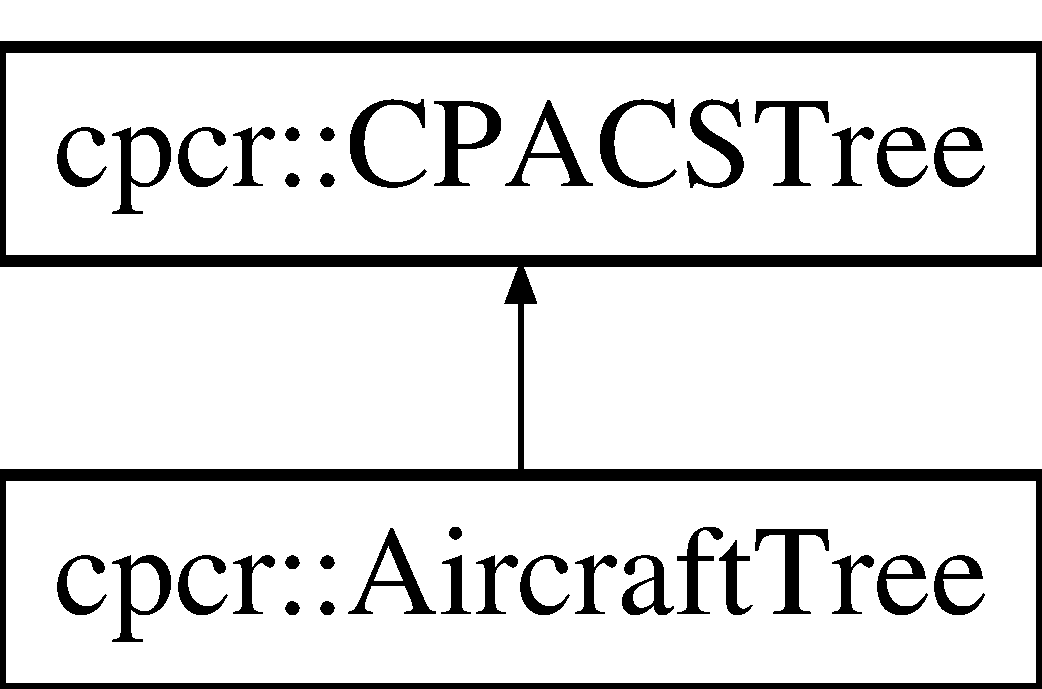
\includegraphics[height=2.000000cm]{classcpcr_1_1CPACSTree}
\end{center}
\end{figure}
\subsection*{Public Member Functions}
\begin{DoxyCompactItemize}
\item 
\hypertarget{classcpcr_1_1CPACSTree_acf68c4bcc9b1252337e1bd086059b7fd}{virtual void {\bfseries build} (std\-::string file, \hyperlink{classcpcr_1_1UniqueXPath}{Unique\-X\-Path} root)}\label{classcpcr_1_1CPACSTree_acf68c4bcc9b1252337e1bd086059b7fd}

\item 
\hypertarget{classcpcr_1_1CPACSTree_a3415e21a201b47eb3b74db22eb8d23c0}{bool {\bfseries is\-Build} ()}\label{classcpcr_1_1CPACSTree_a3415e21a201b47eb3b74db22eb8d23c0}

\item 
\hypertarget{classcpcr_1_1CPACSTree_a6b05f2d3f732821ccdfe7e6d77f183b2}{\hyperlink{classcpcr_1_1CPACSTreeItem}{C\-P\-A\-C\-S\-Tree\-Item} $\ast$ {\bfseries get\-Root} () const }\label{classcpcr_1_1CPACSTree_a6b05f2d3f732821ccdfe7e6d77f183b2}

\item 
\hypertarget{classcpcr_1_1CPACSTree_a1b464498212a24ac5539f38b691ba284}{std\-::string {\bfseries get\-Filename} () const }\label{classcpcr_1_1CPACSTree_a1b464498212a24ac5539f38b691ba284}

\item 
\hypertarget{classcpcr_1_1CPACSTree_a943576f97f72332d988d232484072469}{\hyperlink{classcpcr_1_1CPACSFile}{C\-P\-A\-C\-S\-File} $\ast$ {\bfseries get\-Modifier} ()}\label{classcpcr_1_1CPACSTree_a943576f97f72332d988d232484072469}

\end{DoxyCompactItemize}
\subsection*{Protected Member Functions}
\begin{DoxyCompactItemize}
\item 
\hypertarget{classcpcr_1_1CPACSTree_abb6922e9f4df93d95e74a50af21f3164}{void {\bfseries create\-Children\-Recursively} (\hyperlink{classcpcr_1_1CPACSTreeItem}{C\-P\-A\-C\-S\-Tree\-Item} \&parent)}\label{classcpcr_1_1CPACSTree_abb6922e9f4df93d95e74a50af21f3164}

\item 
\hypertarget{classcpcr_1_1CPACSTree_a81b3b62b69bc5cc1a24f8165edf89717}{void {\bfseries clean} ()}\label{classcpcr_1_1CPACSTree_a81b3b62b69bc5cc1a24f8165edf89717}

\end{DoxyCompactItemize}
\subsection*{Protected Attributes}
\begin{DoxyCompactItemize}
\item 
\hypertarget{classcpcr_1_1CPACSTree_addcd83ebdbcfc2bff3d04f61a3177f1c}{\hyperlink{classcpcr_1_1CPACSFile}{C\-P\-A\-C\-S\-File} {\bfseries modifier}}\label{classcpcr_1_1CPACSTree_addcd83ebdbcfc2bff3d04f61a3177f1c}

\item 
\hypertarget{classcpcr_1_1CPACSTree_a1ad5403c170a393c039603a66a5487fb}{std\-::string {\bfseries file\-Name}}\label{classcpcr_1_1CPACSTree_a1ad5403c170a393c039603a66a5487fb}

\item 
\hypertarget{classcpcr_1_1CPACSTree_aa1c42725557aaf02f79a110406f4363a}{\hyperlink{classcpcr_1_1UniqueXPath}{Unique\-X\-Path} {\bfseries root\-X\-Path}}\label{classcpcr_1_1CPACSTree_aa1c42725557aaf02f79a110406f4363a}

\item 
\hypertarget{classcpcr_1_1CPACSTree_a780500306eb5d3ceeb1e66834233bbcf}{\hyperlink{classcpcr_1_1CPACSTreeItem}{C\-P\-A\-C\-S\-Tree\-Item} $\ast$ {\bfseries m\-\_\-root}}\label{classcpcr_1_1CPACSTree_a780500306eb5d3ceeb1e66834233bbcf}

\item 
\hypertarget{classcpcr_1_1CPACSTree_ad2bda1065fce74df4a72afe6276deef9}{bool {\bfseries m\-\_\-is\-Build}}\label{classcpcr_1_1CPACSTree_ad2bda1065fce74df4a72afe6276deef9}

\end{DoxyCompactItemize}


\subsection{Detailed Description}
Construct and manage a tree structure over C\-P\-A\-C\-S file. 

The xml C\-P\-A\-C\-S format can be represented as a tree. This class create for each xml node starting from the given root a \hyperlink{classcpcr_1_1CPACSTreeItem}{C\-P\-A\-C\-S\-Tree\-Item}. The access to the underlying file is managed by the T\-I\-X\-I library. So basically, this class is a a tree structure that represent the a given xml file from a given root. Remark, that the root need not to be the first element of the C\-P\-A\-C\-S, but can be every where, typically the the \char`\"{}model\-Type\char`\"{} of C\-P\-A\-C\-S can be chosen. 

The documentation for this class was generated from the following files\-:\begin{DoxyCompactItemize}
\item 
/users/disk9/cfse/\-Stage\-\_\-\-Malo/\-C\-P\-A\-C\-S\-Creator\-Lib/\-C\-P\-A\-C\-S\-Creator\-Lib/C\-P\-A\-C\-S\-Tree.\-h\item 
/users/disk9/cfse/\-Stage\-\_\-\-Malo/\-C\-P\-A\-C\-S\-Creator\-Lib/\-C\-P\-A\-C\-S\-Creator\-Lib/C\-P\-A\-C\-S\-Tree.\-cpp\end{DoxyCompactItemize}

\hypertarget{classcpcr_1_1CPACSTreeItem}{\section{cpcr\-:\-:C\-P\-A\-C\-S\-Tree\-Item Class Reference}
\label{classcpcr_1_1CPACSTreeItem}\index{cpcr\-::\-C\-P\-A\-C\-S\-Tree\-Item@{cpcr\-::\-C\-P\-A\-C\-S\-Tree\-Item}}
}
\subsection*{Public Member Functions}
\begin{DoxyCompactItemize}
\item 
\hypertarget{classcpcr_1_1CPACSTreeItem_ac429cedfecfbcf4ffe8545699545be53}{{\bfseries C\-P\-A\-C\-S\-Tree\-Item} (\hyperlink{classcpcr_1_1CPACSTree}{C\-P\-A\-C\-S\-Tree} $\ast$tree, \hyperlink{classcpcr_1_1UniqueXPath}{Unique\-X\-Path} xpath, std\-::string cpacs\-Type, int tixi\-Index, std\-::string uid)}\label{classcpcr_1_1CPACSTreeItem_ac429cedfecfbcf4ffe8545699545be53}

\item 
\hypertarget{classcpcr_1_1CPACSTreeItem_af65aa4fa5c6f78dd06be05f4548c1611}{\hyperlink{classcpcr_1_1CPACSTreeItem}{C\-P\-A\-C\-S\-Tree\-Item} $\ast$ {\bfseries add\-Child} (\hyperlink{classcpcr_1_1UniqueXPath}{Unique\-X\-Path} xpath, std\-::string cpacs\-Type, int tixi\-Index, std\-::string uid)}\label{classcpcr_1_1CPACSTreeItem_af65aa4fa5c6f78dd06be05f4548c1611}

\item 
\hypertarget{classcpcr_1_1CPACSTreeItem_ac3d9050d4eacb0b3a453c20bea489fae}{\hyperlink{classcpcr_1_1CPACSTreeItem}{C\-P\-A\-C\-S\-Tree\-Item} $\ast$ {\bfseries get\-Parent} () const }\label{classcpcr_1_1CPACSTreeItem_ac3d9050d4eacb0b3a453c20bea489fae}

\item 
\hypertarget{classcpcr_1_1CPACSTreeItem_a4eb43b2e19bc43c0ec1bf217acbbf312}{std\-::vector$<$ \hyperlink{classcpcr_1_1CPACSTreeItem}{C\-P\-A\-C\-S\-Tree\-Item} $\ast$ $>$ {\bfseries get\-Children} () const }\label{classcpcr_1_1CPACSTreeItem_a4eb43b2e19bc43c0ec1bf217acbbf312}

\item 
\hypertarget{classcpcr_1_1CPACSTreeItem_a929e21f11dcfabf24ebbbcf00eefccba}{\hyperlink{classcpcr_1_1CPACSTreeItem}{C\-P\-A\-C\-S\-Tree\-Item} $\ast$ {\bfseries get\-Child} (\hyperlink{classcpcr_1_1UniqueXPath}{Unique\-X\-Path} xpath, bool warnings=true)}\label{classcpcr_1_1CPACSTreeItem_a929e21f11dcfabf24ebbbcf00eefccba}

\item 
\hypertarget{classcpcr_1_1CPACSTreeItem_aa9fbcf6e10cefae76c8fdfb19dffc799}{\hyperlink{classcpcr_1_1CPACSTreeItem}{C\-P\-A\-C\-S\-Tree\-Item} $\ast$ {\bfseries get\-Child} (std\-::string xpath\-String, bool warnings=true)}\label{classcpcr_1_1CPACSTreeItem_aa9fbcf6e10cefae76c8fdfb19dffc799}

\item 
\hypertarget{classcpcr_1_1CPACSTreeItem_a7931a73f635081bcaf426fe5c902b45c}{\hyperlink{classcpcr_1_1CPACSTreeItem}{C\-P\-A\-C\-S\-Tree\-Item} $\ast$ {\bfseries get\-Child\-By\-Uid} (std\-::string uid)}\label{classcpcr_1_1CPACSTreeItem_a7931a73f635081bcaf426fe5c902b45c}

\item 
\hypertarget{classcpcr_1_1CPACSTreeItem_aeb542c6aff436a873b9399762a33a651}{\hyperlink{classcpcr_1_1CPACSTreeItem}{C\-P\-A\-C\-S\-Tree\-Item} $\ast$ {\bfseries get\-Parent\-Of\-Type} (std\-::string type)}\label{classcpcr_1_1CPACSTreeItem_aeb542c6aff436a873b9399762a33a651}

\item 
\hypertarget{classcpcr_1_1CPACSTreeItem_ad9bc07d8d0cb9b9a4b77a094c33c9954}{std\-::vector$<$ \hyperlink{classcpcr_1_1CPACSTreeItem}{C\-P\-A\-C\-S\-Tree\-Item} $\ast$ $>$ {\bfseries find\-All\-Children\-Of\-Type\-Recursively} (std\-::string type)}\label{classcpcr_1_1CPACSTreeItem_ad9bc07d8d0cb9b9a4b77a094c33c9954}

\item 
\hypertarget{classcpcr_1_1CPACSTreeItem_acaeb3cb39adec3b66ad3cc4bdd1cffcc}{int {\bfseries position\-Relatively\-To\-Parent} () const }\label{classcpcr_1_1CPACSTreeItem_acaeb3cb39adec3b66ad3cc4bdd1cffcc}

\item 
\hypertarget{classcpcr_1_1CPACSTreeItem_a1aee0b7768a02dfdbf1aec4c5fe41efd}{int {\bfseries get\-Tixi\-Index} () const }\label{classcpcr_1_1CPACSTreeItem_a1aee0b7768a02dfdbf1aec4c5fe41efd}

\item 
\hypertarget{classcpcr_1_1CPACSTreeItem_a9a38c858bae35fb8f762e6341bff4437}{std\-::string {\bfseries get\-Type} () const }\label{classcpcr_1_1CPACSTreeItem_a9a38c858bae35fb8f762e6341bff4437}

\item 
\hypertarget{classcpcr_1_1CPACSTreeItem_a1095a4892526237b54df1c9cfa86211c}{\hyperlink{classcpcr_1_1UniqueXPath}{Unique\-X\-Path} {\bfseries get\-X\-Path} () const }\label{classcpcr_1_1CPACSTreeItem_a1095a4892526237b54df1c9cfa86211c}

\item 
\hypertarget{classcpcr_1_1CPACSTreeItem_a99939b1541ce69714e660f557b2de89d}{std\-::string {\bfseries get\-Uid} () const }\label{classcpcr_1_1CPACSTreeItem_a99939b1541ce69714e660f557b2de89d}

\item 
\hypertarget{classcpcr_1_1CPACSTreeItem_aee254391d09f88ba9cef782ad546bee0}{\hyperlink{classcpcr_1_1CPACSTree}{C\-P\-A\-C\-S\-Tree} $\ast$ {\bfseries get\-Tree} () const }\label{classcpcr_1_1CPACSTreeItem_aee254391d09f88ba9cef782ad546bee0}

\item 
\hypertarget{classcpcr_1_1CPACSTreeItem_a930b692b28895d354d2715517618b4fa}{bool {\bfseries has\-Child\-Of\-Type} (std\-::string name)}\label{classcpcr_1_1CPACSTreeItem_a930b692b28895d354d2715517618b4fa}

\item 
\hypertarget{classcpcr_1_1CPACSTreeItem_a6bd618d2b4bdc9ae87f1ac12b25f0f7c}{std\-::vector$<$ \hyperlink{classcpcr_1_1CPACSTransformation}{C\-P\-A\-C\-S\-Transformation} $>$ {\bfseries compose\-Transform\-Recursively} (\hyperlink{classcpcr_1_1UniqueXPath}{Unique\-X\-Path} target)}\label{classcpcr_1_1CPACSTreeItem_a6bd618d2b4bdc9ae87f1ac12b25f0f7c}

\end{DoxyCompactItemize}


The documentation for this class was generated from the following files\-:\begin{DoxyCompactItemize}
\item 
/users/disk9/cfse/\-Stage\-\_\-\-Malo/\-C\-P\-A\-C\-S\-Creator\-Lib/\-C\-P\-A\-C\-S\-Creator\-Lib/C\-P\-A\-C\-S\-Tree\-Item.\-h\item 
/users/disk9/cfse/\-Stage\-\_\-\-Malo/\-C\-P\-A\-C\-S\-Creator\-Lib/\-C\-P\-A\-C\-S\-Creator\-Lib/C\-P\-A\-C\-S\-Tree\-Item.\-cpp\end{DoxyCompactItemize}

\hypertarget{classel_1_1base_1_1debug_1_1CrashHandler}{\section{el\-:\-:base\-:\-:debug\-:\-:Crash\-Handler Class Reference}
\label{classel_1_1base_1_1debug_1_1CrashHandler}\index{el\-::base\-::debug\-::\-Crash\-Handler@{el\-::base\-::debug\-::\-Crash\-Handler}}
}
\subsection*{Public Member Functions}
\begin{DoxyCompactItemize}
\item 
\hypertarget{classel_1_1base_1_1debug_1_1CrashHandler_a74248809ad31620248a0ee60a5fe9894}{{\bfseries Crash\-Handler} (bool)}\label{classel_1_1base_1_1debug_1_1CrashHandler_a74248809ad31620248a0ee60a5fe9894}

\end{DoxyCompactItemize}


The documentation for this class was generated from the following file\-:\begin{DoxyCompactItemize}
\item 
/users/disk9/cfse/\-Stage\-\_\-\-Malo/\-C\-P\-A\-C\-S\-Creator\-Lib/\-C\-P\-A\-C\-S\-Creator\-Lib/easylogging++.\-h\end{DoxyCompactItemize}

\hypertarget{classCreatorException}{\section{Creator\-Exception Class Reference}
\label{classCreatorException}\index{Creator\-Exception@{Creator\-Exception}}
}
Inheritance diagram for Creator\-Exception\-:\begin{figure}[H]
\begin{center}
\leavevmode
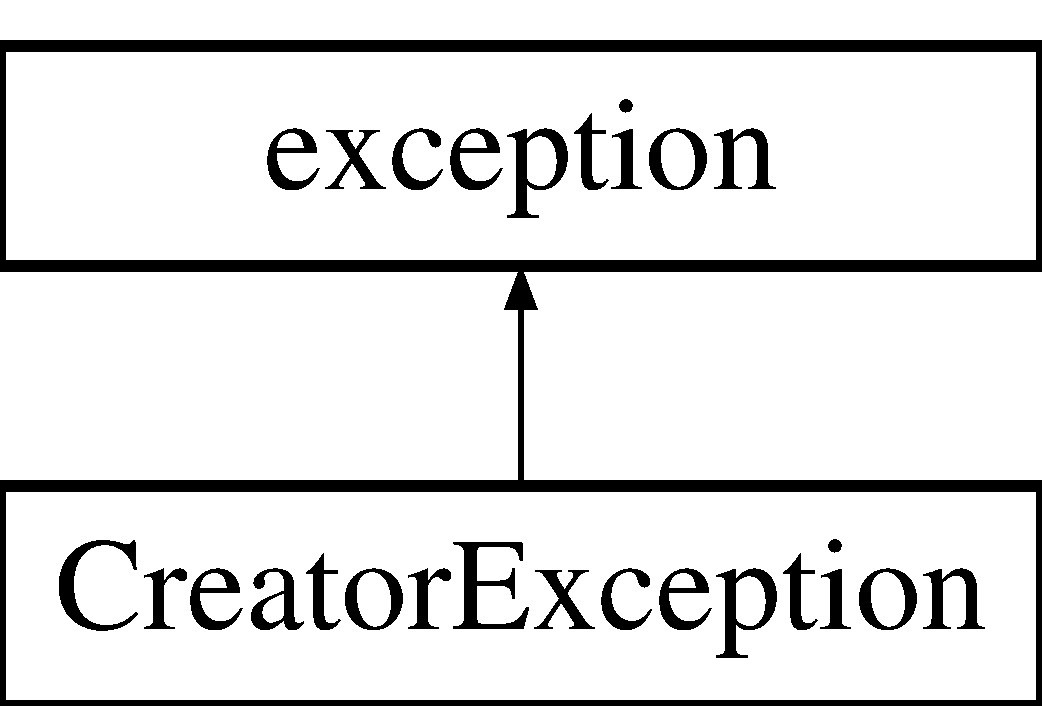
\includegraphics[height=2.000000cm]{classCreatorException}
\end{center}
\end{figure}
\subsection*{Public Member Functions}
\begin{DoxyCompactItemize}
\item 
\hypertarget{classCreatorException_ae77e43c3b0906d16f1f0fb02fc13ec1b}{{\bfseries Creator\-Exception} (const std\-::string \&msg, int err\-Num=-\/1)}\label{classCreatorException_ae77e43c3b0906d16f1f0fb02fc13ec1b}

\item 
\hypertarget{classCreatorException_a12dddef6d880bbd5d171debdea0bae17}{virtual const char $\ast$ {\bfseries what} () const   throw ()}\label{classCreatorException_a12dddef6d880bbd5d171debdea0bae17}

\item 
\hypertarget{classCreatorException_a153befd4e3cd6016fd3c5719e6deac28}{void {\bfseries add\-To\-Message} (const std\-::string \&msg)}\label{classCreatorException_a153befd4e3cd6016fd3c5719e6deac28}

\end{DoxyCompactItemize}
\subsection*{Public Attributes}
\begin{DoxyCompactItemize}
\item 
\hypertarget{classCreatorException_a27b5d0e83422ad885ea701f38a23644e}{int {\bfseries err\-Number}}\label{classCreatorException_a27b5d0e83422ad885ea701f38a23644e}

\end{DoxyCompactItemize}


The documentation for this class was generated from the following files\-:\begin{DoxyCompactItemize}
\item 
/users/disk9/cfse/\-Stage\-\_\-\-Malo/\-C\-P\-A\-C\-S\-Creator\-Lib/\-C\-P\-A\-C\-S\-Creator\-Lib/Creator\-Exception.\-h\item 
/users/disk9/cfse/\-Stage\-\_\-\-Malo/\-C\-P\-A\-C\-S\-Creator\-Lib/\-C\-P\-A\-C\-S\-Creator\-Lib/Creator\-Exception.\-cpp\end{DoxyCompactItemize}

\hypertarget{classel_1_1CustomFormatSpecifier}{\section{el\-:\-:Custom\-Format\-Specifier Class Reference}
\label{classel_1_1CustomFormatSpecifier}\index{el\-::\-Custom\-Format\-Specifier@{el\-::\-Custom\-Format\-Specifier}}
}


User-\/provided custom format specifier.  




{\ttfamily \#include $<$easylogging++.\-h$>$}

\subsection*{Public Member Functions}
\begin{DoxyCompactItemize}
\item 
\hypertarget{classel_1_1CustomFormatSpecifier_a1d1bfa8b489d2908ee543023a51e58f6}{{\bfseries Custom\-Format\-Specifier} (const char $\ast$format\-Specifier, const \hyperlink{namespaceel_a7127f2de2769e2a199a3665f42028a16}{Format\-Specifier\-Value\-Resolver} \&resolver)}\label{classel_1_1CustomFormatSpecifier_a1d1bfa8b489d2908ee543023a51e58f6}

\item 
\hypertarget{classel_1_1CustomFormatSpecifier_a0be00787b7ca1caedd32e1627d76fd24}{const char $\ast$ {\bfseries format\-Specifier} (void) const }\label{classel_1_1CustomFormatSpecifier_a0be00787b7ca1caedd32e1627d76fd24}

\item 
\hypertarget{classel_1_1CustomFormatSpecifier_ac426e6771ae35e060313b8683b88adc8}{const \\*
\hyperlink{namespaceel_a7127f2de2769e2a199a3665f42028a16}{Format\-Specifier\-Value\-Resolver} \& {\bfseries resolver} (void) const }\label{classel_1_1CustomFormatSpecifier_ac426e6771ae35e060313b8683b88adc8}

\item 
\hypertarget{classel_1_1CustomFormatSpecifier_ae17a9fbf8c5a28867308fcb8966a3aa0}{bool {\bfseries operator==} (const char $\ast$format\-Specifier)}\label{classel_1_1CustomFormatSpecifier_ae17a9fbf8c5a28867308fcb8966a3aa0}

\end{DoxyCompactItemize}


\subsection{Detailed Description}
User-\/provided custom format specifier. 

\begin{DoxySeeAlso}{See Also}
\hyperlink{classel_1_1Helpers_aa6de15a09db4f2a6763a6652c0ea12b1}{el\-::\-Helpers\-::install\-Custom\-Format\-Specifier} 

\hyperlink{namespaceel_a7127f2de2769e2a199a3665f42028a16}{Format\-Specifier\-Value\-Resolver} 
\end{DoxySeeAlso}


The documentation for this class was generated from the following file\-:\begin{DoxyCompactItemize}
\item 
/users/disk9/cfse/\-Stage\-\_\-\-Malo/\-C\-P\-A\-C\-S\-Creator\-Lib/\-C\-P\-A\-C\-S\-Creator\-Lib/easylogging++.\-h\end{DoxyCompactItemize}

\hypertarget{classel_1_1base_1_1utils_1_1DateTime}{\section{el\-:\-:base\-:\-:utils\-:\-:Date\-Time Class Reference}
\label{classel_1_1base_1_1utils_1_1DateTime}\index{el\-::base\-::utils\-::\-Date\-Time@{el\-::base\-::utils\-::\-Date\-Time}}
}


Contains utilities for cross-\/platform date/time. This class make use of \hyperlink{classel_1_1base_1_1utils_1_1Str}{el\-::base\-::utils\-::\-Str}.  




{\ttfamily \#include $<$easylogging++.\-h$>$}

Inheritance diagram for el\-:\-:base\-:\-:utils\-:\-:Date\-Time\-:\begin{figure}[H]
\begin{center}
\leavevmode
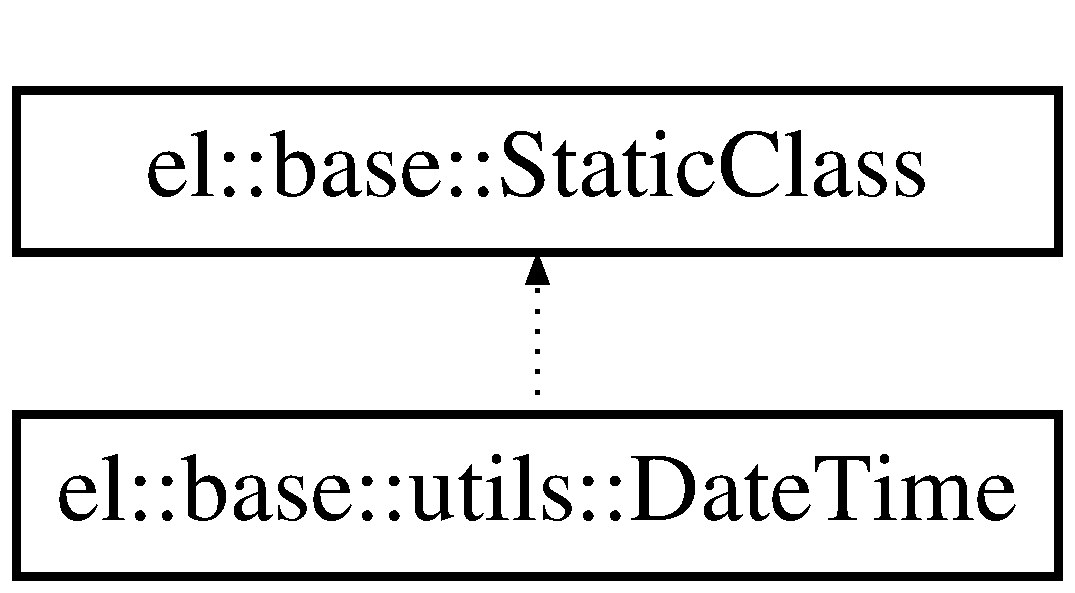
\includegraphics[height=2.000000cm]{classel_1_1base_1_1utils_1_1DateTime}
\end{center}
\end{figure}
\subsection*{Static Public Member Functions}
\begin{DoxyCompactItemize}
\item 
static void \hyperlink{classel_1_1base_1_1utils_1_1DateTime_ac000e6ecf705c2194a173d618ff4acfd}{gettimeofday} (struct timeval $\ast$tv)
\begin{DoxyCompactList}\small\item\em Cross platform gettimeofday for Windows and unix platform. This can be used to determine current microsecond. \end{DoxyCompactList}\item 
static std\-::string \hyperlink{classel_1_1base_1_1utils_1_1DateTime_afdbf02ed83d6312d63b0f3d114a44393}{get\-Date\-Time} (const char $\ast$format, const \hyperlink{classel_1_1base_1_1SubsecondPrecision}{base\-::\-Subsecond\-Precision} $\ast$ss\-Prec)
\begin{DoxyCompactList}\small\item\em Gets current date and time with a subsecond part. \end{DoxyCompactList}\item 
\hypertarget{classel_1_1base_1_1utils_1_1DateTime_a18d429b13ddeece5eaf0cee1a6f9e7bf}{static std\-::string \hyperlink{classel_1_1base_1_1utils_1_1DateTime_a18d429b13ddeece5eaf0cee1a6f9e7bf}{timeval\-To\-String} (struct timeval tval, const char $\ast$format, const \hyperlink{classel_1_1base_1_1SubsecondPrecision}{el\-::base\-::\-Subsecond\-Precision} $\ast$ss\-Prec)}\label{classel_1_1base_1_1utils_1_1DateTime_a18d429b13ddeece5eaf0cee1a6f9e7bf}

\begin{DoxyCompactList}\small\item\em Converts timeval (struct from ctime) to string using specified format and subsecond precision. \end{DoxyCompactList}\item 
\hypertarget{classel_1_1base_1_1utils_1_1DateTime_a1eea58fffe291c969a526d08515d29d7}{static base\-::type\-::string\-\_\-t \hyperlink{classel_1_1base_1_1utils_1_1DateTime_a1eea58fffe291c969a526d08515d29d7}{format\-Time} (unsigned long long time, \hyperlink{namespaceel_1_1base_a1b886858c6409097395b24b1bdf03c39}{base\-::\-Timestamp\-Unit} timestamp\-Unit)}\label{classel_1_1base_1_1utils_1_1DateTime_a1eea58fffe291c969a526d08515d29d7}

\begin{DoxyCompactList}\small\item\em Formats time to get unit accordingly, units like second if $>$ 1000 or minutes if $>$ 60000 etc. \end{DoxyCompactList}\item 
\hypertarget{classel_1_1base_1_1utils_1_1DateTime_a9181a3544442e1d3c05d8c96bbfff16d}{static unsigned long long \hyperlink{classel_1_1base_1_1utils_1_1DateTime_a9181a3544442e1d3c05d8c96bbfff16d}{get\-Time\-Difference} (const struct timeval \&end\-Time, const struct timeval \&start\-Time, \hyperlink{namespaceel_1_1base_a1b886858c6409097395b24b1bdf03c39}{base\-::\-Timestamp\-Unit} timestamp\-Unit)}\label{classel_1_1base_1_1utils_1_1DateTime_a9181a3544442e1d3c05d8c96bbfff16d}

\begin{DoxyCompactList}\small\item\em Gets time difference in milli/micro second depending on timestamp\-Unit. \end{DoxyCompactList}\item 
\hypertarget{classel_1_1base_1_1utils_1_1DateTime_a71125138b2ee3e400b7b89f4001f2887}{static struct\-::tm $\ast$ {\bfseries build\-Time\-Info} (struct timeval $\ast$curr\-Time, struct\-::tm $\ast$time\-Info)}\label{classel_1_1base_1_1utils_1_1DateTime_a71125138b2ee3e400b7b89f4001f2887}

\end{DoxyCompactItemize}


\subsection{Detailed Description}
Contains utilities for cross-\/platform date/time. This class make use of \hyperlink{classel_1_1base_1_1utils_1_1Str}{el\-::base\-::utils\-::\-Str}. 

\subsection{Member Function Documentation}
\hypertarget{classel_1_1base_1_1utils_1_1DateTime_afdbf02ed83d6312d63b0f3d114a44393}{\index{el\-::base\-::utils\-::\-Date\-Time@{el\-::base\-::utils\-::\-Date\-Time}!get\-Date\-Time@{get\-Date\-Time}}
\index{get\-Date\-Time@{get\-Date\-Time}!el::base::utils::DateTime@{el\-::base\-::utils\-::\-Date\-Time}}
\subsubsection[{get\-Date\-Time}]{\setlength{\rightskip}{0pt plus 5cm}static std\-::string el\-::base\-::utils\-::\-Date\-Time\-::get\-Date\-Time (
\begin{DoxyParamCaption}
\item[{const char $\ast$}]{format, }
\item[{const {\bf base\-::\-Subsecond\-Precision} $\ast$}]{ss\-Prec}
\end{DoxyParamCaption}
)\hspace{0.3cm}{\ttfamily [static]}}}\label{classel_1_1base_1_1utils_1_1DateTime_afdbf02ed83d6312d63b0f3d114a44393}


Gets current date and time with a subsecond part. 


\begin{DoxyParams}{Parameters}
{\em format} & User provided date/time format \\
\hline
{\em ss\-Prec} & A pointer to \hyperlink{classel_1_1base_1_1SubsecondPrecision}{base\-::\-Subsecond\-Precision} from configuration (non-\/null) \\
\hline
\end{DoxyParams}
\begin{DoxyReturn}{Returns}
string based date time in specified format. 
\end{DoxyReturn}
\hypertarget{classel_1_1base_1_1utils_1_1DateTime_ac000e6ecf705c2194a173d618ff4acfd}{\index{el\-::base\-::utils\-::\-Date\-Time@{el\-::base\-::utils\-::\-Date\-Time}!gettimeofday@{gettimeofday}}
\index{gettimeofday@{gettimeofday}!el::base::utils::DateTime@{el\-::base\-::utils\-::\-Date\-Time}}
\subsubsection[{gettimeofday}]{\setlength{\rightskip}{0pt plus 5cm}static void el\-::base\-::utils\-::\-Date\-Time\-::gettimeofday (
\begin{DoxyParamCaption}
\item[{struct timeval $\ast$}]{tv}
\end{DoxyParamCaption}
)\hspace{0.3cm}{\ttfamily [static]}}}\label{classel_1_1base_1_1utils_1_1DateTime_ac000e6ecf705c2194a173d618ff4acfd}


Cross platform gettimeofday for Windows and unix platform. This can be used to determine current microsecond. 

For unix system it uses gettimeofday(timeval$\ast$, timezone$\ast$) and for Windows, a seperate implementation is provided 
\begin{DoxyParams}[1]{Parameters}
\mbox{\tt in,out}  & {\em tv} & Pointer that gets updated \\
\hline
\end{DoxyParams}


The documentation for this class was generated from the following file\-:\begin{DoxyCompactItemize}
\item 
/users/disk9/cfse/\-Stage\-\_\-\-Malo/\-C\-P\-A\-C\-S\-Creator\-Lib/\-C\-P\-A\-C\-S\-Creator\-Lib/easylogging++.\-h\end{DoxyCompactItemize}

\hypertarget{classel_1_1base_1_1DefaultLogBuilder}{\section{el\-:\-:base\-:\-:Default\-Log\-Builder Class Reference}
\label{classel_1_1base_1_1DefaultLogBuilder}\index{el\-::base\-::\-Default\-Log\-Builder@{el\-::base\-::\-Default\-Log\-Builder}}
}
Inheritance diagram for el\-:\-:base\-:\-:Default\-Log\-Builder\-:\begin{figure}[H]
\begin{center}
\leavevmode
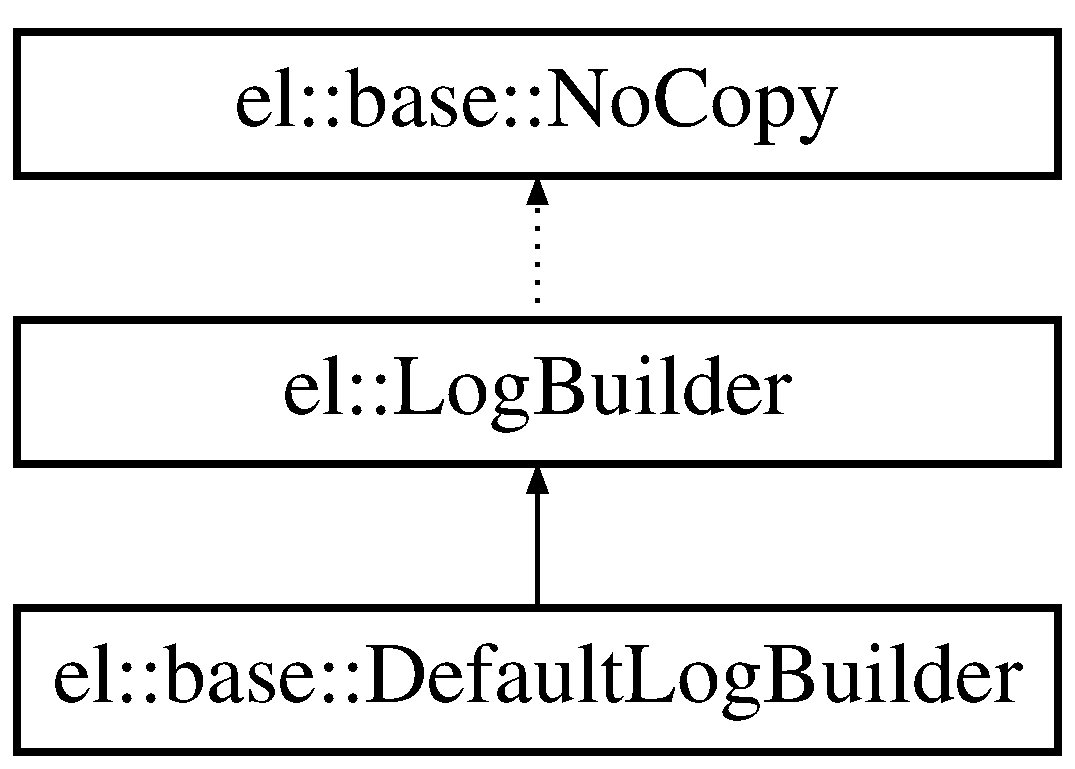
\includegraphics[height=3.000000cm]{classel_1_1base_1_1DefaultLogBuilder}
\end{center}
\end{figure}
\subsection*{Public Member Functions}
\begin{DoxyCompactItemize}
\item 
\hypertarget{classel_1_1base_1_1DefaultLogBuilder_aa8d2f42068115d899ed81de1b0ed360e}{base\-::type\-::string\-\_\-t {\bfseries build} (const \hyperlink{classel_1_1LogMessage}{Log\-Message} $\ast$log\-Message, bool append\-New\-Line) const }\label{classel_1_1base_1_1DefaultLogBuilder_aa8d2f42068115d899ed81de1b0ed360e}

\end{DoxyCompactItemize}


The documentation for this class was generated from the following file\-:\begin{DoxyCompactItemize}
\item 
/users/disk9/cfse/\-Stage\-\_\-\-Malo/\-C\-P\-A\-C\-S\-Creator\-Lib/\-C\-P\-A\-C\-S\-Creator\-Lib/easylogging++.\-h\end{DoxyCompactItemize}

\hypertarget{classel_1_1base_1_1DefaultLogDispatchCallback}{\section{el\-:\-:base\-:\-:Default\-Log\-Dispatch\-Callback Class Reference}
\label{classel_1_1base_1_1DefaultLogDispatchCallback}\index{el\-::base\-::\-Default\-Log\-Dispatch\-Callback@{el\-::base\-::\-Default\-Log\-Dispatch\-Callback}}
}
Inheritance diagram for el\-:\-:base\-:\-:Default\-Log\-Dispatch\-Callback\-:\begin{figure}[H]
\begin{center}
\leavevmode
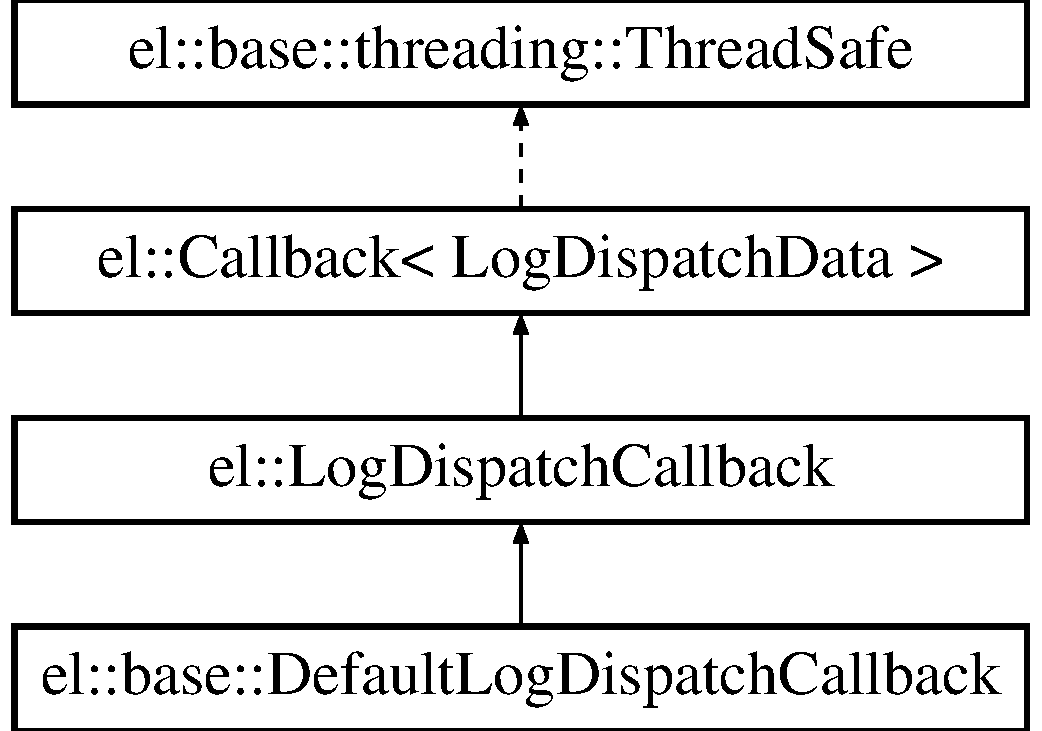
\includegraphics[height=4.000000cm]{classel_1_1base_1_1DefaultLogDispatchCallback}
\end{center}
\end{figure}
\subsection*{Protected Member Functions}
\begin{DoxyCompactItemize}
\item 
\hypertarget{classel_1_1base_1_1DefaultLogDispatchCallback_acdac30f202c245500e6d94c55eee6d95}{void {\bfseries handle} (const \hyperlink{classel_1_1LogDispatchData}{Log\-Dispatch\-Data} $\ast$data)}\label{classel_1_1base_1_1DefaultLogDispatchCallback_acdac30f202c245500e6d94c55eee6d95}

\end{DoxyCompactItemize}
\subsection*{Additional Inherited Members}


The documentation for this class was generated from the following file\-:\begin{DoxyCompactItemize}
\item 
/users/disk9/cfse/\-Stage\-\_\-\-Malo/\-C\-P\-A\-C\-S\-Creator\-Lib/\-C\-P\-A\-C\-S\-Creator\-Lib/easylogging++.\-h\end{DoxyCompactItemize}

\hypertarget{classel_1_1base_1_1utils_1_1File}{\section{el\-:\-:base\-:\-:utils\-:\-:File Class Reference}
\label{classel_1_1base_1_1utils_1_1File}\index{el\-::base\-::utils\-::\-File@{el\-::base\-::utils\-::\-File}}
}
Inheritance diagram for el\-:\-:base\-:\-:utils\-:\-:File\-:\begin{figure}[H]
\begin{center}
\leavevmode
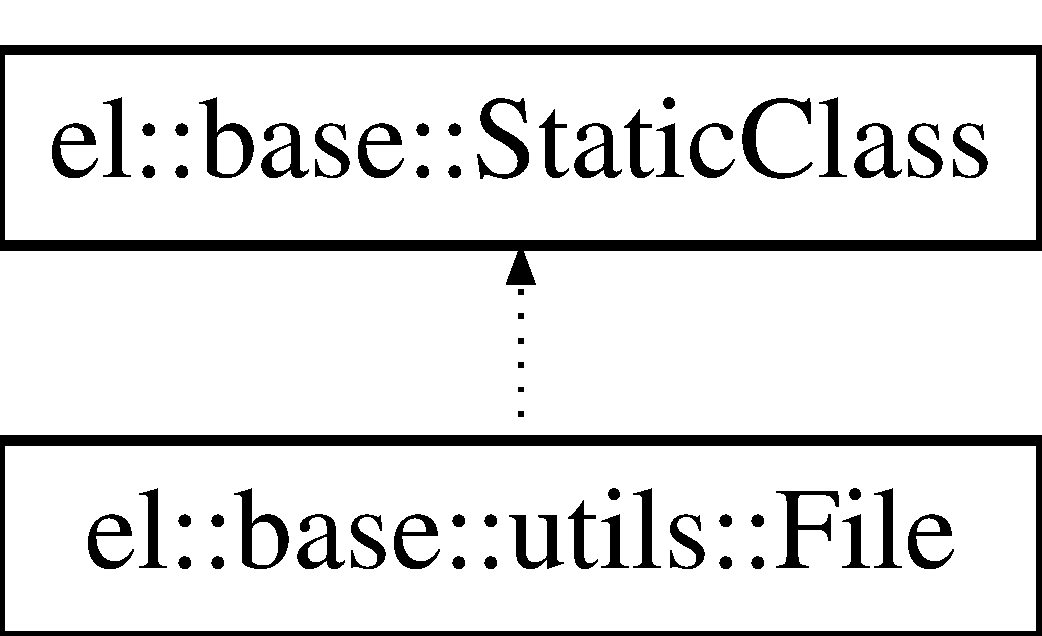
\includegraphics[height=2.000000cm]{classel_1_1base_1_1utils_1_1File}
\end{center}
\end{figure}
\subsection*{Static Public Member Functions}
\begin{DoxyCompactItemize}
\item 
static base\-::type\-::fstream\-\_\-t $\ast$ \hyperlink{classel_1_1base_1_1utils_1_1File_aa4bef1f2e00269d75c1c1eabb0ce4563}{new\-File\-Stream} (const std\-::string \&filename)
\begin{DoxyCompactList}\small\item\em Creates new out file stream for specified filename. \end{DoxyCompactList}\item 
\hypertarget{classel_1_1base_1_1utils_1_1File_a54415ba02f698ba978795265f7f4b86c}{static std\-::size\-\_\-t \hyperlink{classel_1_1base_1_1utils_1_1File_a54415ba02f698ba978795265f7f4b86c}{get\-Size\-Of\-File} (base\-::type\-::fstream\-\_\-t $\ast$fs)}\label{classel_1_1base_1_1utils_1_1File_a54415ba02f698ba978795265f7f4b86c}

\begin{DoxyCompactList}\small\item\em Gets size of file provided in stream. \end{DoxyCompactList}\item 
\hypertarget{classel_1_1base_1_1utils_1_1File_a4fc9e36b814f1aeaa4931e35d58e5b45}{static bool \hyperlink{classel_1_1base_1_1utils_1_1File_a4fc9e36b814f1aeaa4931e35d58e5b45}{path\-Exists} (const char $\ast$path, bool consider\-File=false)}\label{classel_1_1base_1_1utils_1_1File_a4fc9e36b814f1aeaa4931e35d58e5b45}

\begin{DoxyCompactList}\small\item\em Determines whether or not provided path exist in current file system. \end{DoxyCompactList}\item 
static bool \hyperlink{classel_1_1base_1_1utils_1_1File_a34fbb5b06201c7e3db71db80e017fb96}{create\-Path} (const std\-::string \&path)
\begin{DoxyCompactList}\small\item\em Creates specified path on file system. \end{DoxyCompactList}\item 
\hypertarget{classel_1_1base_1_1utils_1_1File_af541c62ed408de7e368d339f96c0c6cf}{static std\-::string \hyperlink{classel_1_1base_1_1utils_1_1File_af541c62ed408de7e368d339f96c0c6cf}{extract\-Path\-From\-Filename} (const std\-::string \&full\-Path, const char $\ast$seperator=base\-::consts\-::k\-File\-Path\-Seperator)}\label{classel_1_1base_1_1utils_1_1File_af541c62ed408de7e368d339f96c0c6cf}

\begin{DoxyCompactList}\small\item\em Extracts path of filename with leading slash. \end{DoxyCompactList}\item 
\hypertarget{classel_1_1base_1_1utils_1_1File_a38e3b3c72f73de47563b289eff13ae2d}{static void \hyperlink{classel_1_1base_1_1utils_1_1File_a38e3b3c72f73de47563b289eff13ae2d}{build\-Stripped\-Filename} (const char $\ast$filename, char buff\mbox{[}$\,$\mbox{]}, std\-::size\-\_\-t limit=base\-::consts\-::k\-Source\-Filename\-Max\-Length)}\label{classel_1_1base_1_1utils_1_1File_a38e3b3c72f73de47563b289eff13ae2d}

\begin{DoxyCompactList}\small\item\em builds stripped filename and puts it in buff \end{DoxyCompactList}\item 
\hypertarget{classel_1_1base_1_1utils_1_1File_ad6c3703c16b95bd4992f501380d503b4}{static void \hyperlink{classel_1_1base_1_1utils_1_1File_ad6c3703c16b95bd4992f501380d503b4}{build\-Base\-Filename} (const std\-::string \&full\-Path, char buff\mbox{[}$\,$\mbox{]}, std\-::size\-\_\-t limit=base\-::consts\-::k\-Source\-Filename\-Max\-Length, const char $\ast$seperator=base\-::consts\-::k\-File\-Path\-Seperator)}\label{classel_1_1base_1_1utils_1_1File_ad6c3703c16b95bd4992f501380d503b4}

\begin{DoxyCompactList}\small\item\em builds base filename and puts it in buff \end{DoxyCompactList}\end{DoxyCompactItemize}


\subsection{Member Function Documentation}
\hypertarget{classel_1_1base_1_1utils_1_1File_a34fbb5b06201c7e3db71db80e017fb96}{\index{el\-::base\-::utils\-::\-File@{el\-::base\-::utils\-::\-File}!create\-Path@{create\-Path}}
\index{create\-Path@{create\-Path}!el::base::utils::File@{el\-::base\-::utils\-::\-File}}
\subsubsection[{create\-Path}]{\setlength{\rightskip}{0pt plus 5cm}static bool el\-::base\-::utils\-::\-File\-::create\-Path (
\begin{DoxyParamCaption}
\item[{const std\-::string \&}]{path}
\end{DoxyParamCaption}
)\hspace{0.3cm}{\ttfamily [static]}}}\label{classel_1_1base_1_1utils_1_1File_a34fbb5b06201c7e3db71db80e017fb96}


Creates specified path on file system. 


\begin{DoxyParams}{Parameters}
{\em path} & Path to create. \\
\hline
\end{DoxyParams}
\hypertarget{classel_1_1base_1_1utils_1_1File_aa4bef1f2e00269d75c1c1eabb0ce4563}{\index{el\-::base\-::utils\-::\-File@{el\-::base\-::utils\-::\-File}!new\-File\-Stream@{new\-File\-Stream}}
\index{new\-File\-Stream@{new\-File\-Stream}!el::base::utils::File@{el\-::base\-::utils\-::\-File}}
\subsubsection[{new\-File\-Stream}]{\setlength{\rightskip}{0pt plus 5cm}static base\-::type\-::fstream\-\_\-t$\ast$ el\-::base\-::utils\-::\-File\-::new\-File\-Stream (
\begin{DoxyParamCaption}
\item[{const std\-::string \&}]{filename}
\end{DoxyParamCaption}
)\hspace{0.3cm}{\ttfamily [static]}}}\label{classel_1_1base_1_1utils_1_1File_aa4bef1f2e00269d75c1c1eabb0ce4563}


Creates new out file stream for specified filename. 

\begin{DoxyReturn}{Returns}
Pointer to newly created fstream or nullptr 
\end{DoxyReturn}


The documentation for this class was generated from the following file\-:\begin{DoxyCompactItemize}
\item 
/users/disk9/cfse/\-Stage\-\_\-\-Malo/\-C\-P\-A\-C\-S\-Creator\-Lib/\-C\-P\-A\-C\-S\-Creator\-Lib/easylogging++.\-h\end{DoxyCompactItemize}

\hypertarget{structstd_1_1hash_3_01el_1_1Level_01_4}{\section{std\-:\-:hash$<$ el\-:\-:Level $>$ Struct Template Reference}
\label{structstd_1_1hash_3_01el_1_1Level_01_4}\index{std\-::hash$<$ el\-::\-Level $>$@{std\-::hash$<$ el\-::\-Level $>$}}
}
\subsection*{Public Member Functions}
\begin{DoxyCompactItemize}
\item 
\hypertarget{structstd_1_1hash_3_01el_1_1Level_01_4_a534496ed916cbc46814822bc0dc1e210}{std\-::size\-\_\-t {\bfseries operator()} (const \hyperlink{namespaceel_ab0ac6091262344c52dd2d3ad099e8e36}{el\-::\-Level} \&l) const }\label{structstd_1_1hash_3_01el_1_1Level_01_4_a534496ed916cbc46814822bc0dc1e210}

\end{DoxyCompactItemize}


The documentation for this struct was generated from the following file\-:\begin{DoxyCompactItemize}
\item 
/users/disk9/cfse/\-Stage\-\_\-\-Malo/\-C\-P\-A\-C\-S\-Creator\-Lib/\-C\-P\-A\-C\-S\-Creator\-Lib/easylogging++.\-h\end{DoxyCompactItemize}

\hypertarget{classel_1_1Helpers}{\section{el\-:\-:Helpers Class Reference}
\label{classel_1_1Helpers}\index{el\-::\-Helpers@{el\-::\-Helpers}}
}


Static helpers for developers.  




{\ttfamily \#include $<$easylogging++.\-h$>$}

Inheritance diagram for el\-:\-:Helpers\-:\begin{figure}[H]
\begin{center}
\leavevmode
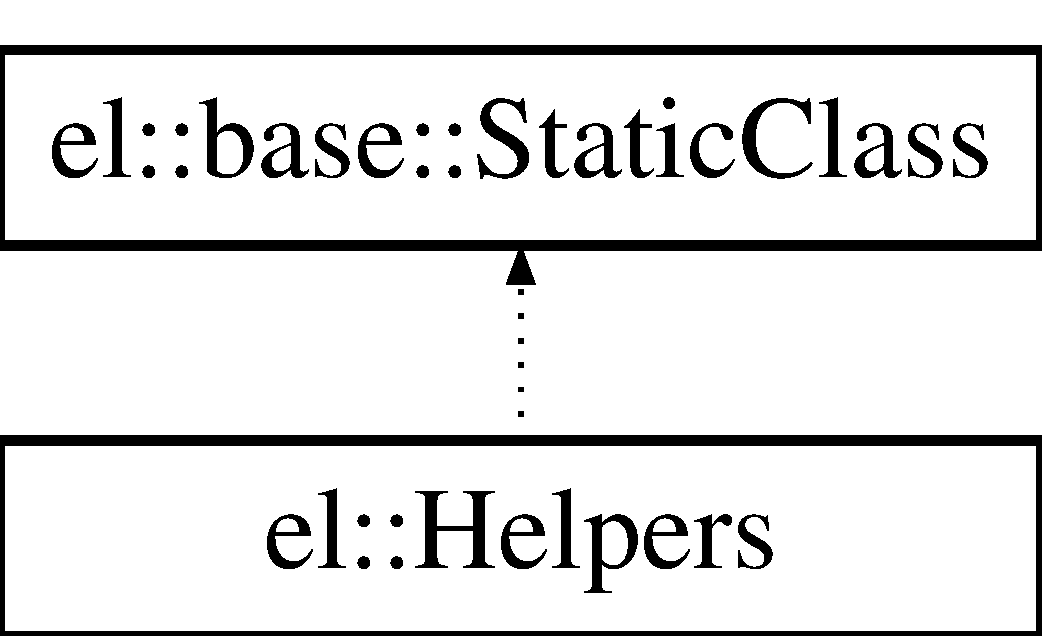
\includegraphics[height=2.000000cm]{classel_1_1Helpers}
\end{center}
\end{figure}
\subsection*{Static Public Member Functions}
\begin{DoxyCompactItemize}
\item 
\hypertarget{classel_1_1Helpers_af78fd39725281e3dddd7c0fbdc14f11f}{static void \hyperlink{classel_1_1Helpers_af78fd39725281e3dddd7c0fbdc14f11f}{set\-Storage} (base\-::type\-::\-Storage\-Pointer \hyperlink{classel_1_1Helpers_a13a5365de36b3af27660cf9b358829d3}{storage})}\label{classel_1_1Helpers_af78fd39725281e3dddd7c0fbdc14f11f}

\begin{DoxyCompactList}\small\item\em Shares logging repository (\hyperlink{classel_1_1base_1_1Storage}{base\-::\-Storage}) \end{DoxyCompactList}\item 
static base\-::type\-::\-Storage\-Pointer \hyperlink{classel_1_1Helpers_a13a5365de36b3af27660cf9b358829d3}{storage} ()
\item 
\hypertarget{classel_1_1Helpers_a68748f618a0c2840b96dc12532b09bf0}{static void \hyperlink{classel_1_1Helpers_a68748f618a0c2840b96dc12532b09bf0}{set\-Args} (int argc, char $\ast$$\ast$argv)}\label{classel_1_1Helpers_a68748f618a0c2840b96dc12532b09bf0}

\begin{DoxyCompactList}\small\item\em Sets application arguments and figures out whats active for logging and whats not. \end{DoxyCompactList}\item 
static void \hyperlink{classel_1_1Helpers_afac7a023e2c13a62d0295cf0239eb848}{set\-Args} (int argc, const char $\ast$$\ast$argv)
\begin{DoxyCompactList}\small\item\em Sets application arguments and figures out whats active for logging and whats not. \end{DoxyCompactList}\item 
\hypertarget{classel_1_1Helpers_a315250270334214c2749398feba08863}{static void \hyperlink{classel_1_1Helpers_a315250270334214c2749398feba08863}{set\-Thread\-Name} (const std\-::string \&name)}\label{classel_1_1Helpers_a315250270334214c2749398feba08863}

\begin{DoxyCompactList}\small\item\em Sets thread name for current thread. Requires std\-::thread. \end{DoxyCompactList}\item 
\hypertarget{classel_1_1Helpers_ae19cb3baa6d8081a9e922736a384f70b}{static std\-::string {\bfseries get\-Thread\-Name} ()}\label{classel_1_1Helpers_ae19cb3baa6d8081a9e922736a384f70b}

\item 
\hypertarget{classel_1_1Helpers_a5fd7ad6d636c28d2e706203d0c43cf8c}{static void \hyperlink{classel_1_1Helpers_a5fd7ad6d636c28d2e706203d0c43cf8c}{install\-Pre\-Roll\-Out\-Callback} (const Pre\-Roll\-Out\-Callback \&callback)}\label{classel_1_1Helpers_a5fd7ad6d636c28d2e706203d0c43cf8c}

\begin{DoxyCompactList}\small\item\em Installs pre rollout callback, this callback is triggered when log file is about to be rolled out (can be useful for backing up) \end{DoxyCompactList}\item 
\hypertarget{classel_1_1Helpers_ab829e5ed1b43bf965f5c288bc0280376}{static void \hyperlink{classel_1_1Helpers_ab829e5ed1b43bf965f5c288bc0280376}{uninstall\-Pre\-Roll\-Out\-Callback} (void)}\label{classel_1_1Helpers_ab829e5ed1b43bf965f5c288bc0280376}

\begin{DoxyCompactList}\small\item\em Uninstalls pre rollout callback. \end{DoxyCompactList}\item 
\hypertarget{classel_1_1Helpers_a3f3e84057567a8ac568a35899318544a}{{\footnotesize template$<$typename T $>$ }\\static bool \hyperlink{classel_1_1Helpers_a3f3e84057567a8ac568a35899318544a}{install\-Log\-Dispatch\-Callback} (const std\-::string \&id)}\label{classel_1_1Helpers_a3f3e84057567a8ac568a35899318544a}

\begin{DoxyCompactList}\small\item\em Installs post log dispatch callback, this callback is triggered when log is dispatched. \end{DoxyCompactList}\item 
\hypertarget{classel_1_1Helpers_ac94b44cc8d399a5842703126478300d7}{{\footnotesize template$<$typename T $>$ }\\static void \hyperlink{classel_1_1Helpers_ac94b44cc8d399a5842703126478300d7}{uninstall\-Log\-Dispatch\-Callback} (const std\-::string \&id)}\label{classel_1_1Helpers_ac94b44cc8d399a5842703126478300d7}

\begin{DoxyCompactList}\small\item\em Uninstalls log dispatch callback. \end{DoxyCompactList}\item 
\hypertarget{classel_1_1Helpers_aa01d59ca141bc75c4fdd78a34234611b}{{\footnotesize template$<$typename T $>$ }\\static T $\ast$ {\bfseries log\-Dispatch\-Callback} (const std\-::string \&id)}\label{classel_1_1Helpers_aa01d59ca141bc75c4fdd78a34234611b}

\item 
\hypertarget{classel_1_1Helpers_a8b032e32cd042ddc4fef4e814bad1082}{{\footnotesize template$<$typename T $>$ }\\static std\-::string \hyperlink{classel_1_1Helpers_a8b032e32cd042ddc4fef4e814bad1082}{convert\-Template\-To\-Std\-String} (const T \&templ)}\label{classel_1_1Helpers_a8b032e32cd042ddc4fef4e814bad1082}

\begin{DoxyCompactList}\small\item\em Converts template to std\-::string -\/ useful for loggable classes to log containers within log(std\-::ostream\&) const. \end{DoxyCompactList}\item 
\hypertarget{classel_1_1Helpers_a83bab44f77a4961f8f5231e7ce9917bb}{static const \\*
\hyperlink{classel_1_1base_1_1utils_1_1CommandLineArgs}{el\-::base\-::utils\-::\-Command\-Line\-Args} $\ast$ \hyperlink{classel_1_1Helpers_a83bab44f77a4961f8f5231e7ce9917bb}{command\-Line\-Args} (void)}\label{classel_1_1Helpers_a83bab44f77a4961f8f5231e7ce9917bb}

\begin{DoxyCompactList}\small\item\em Returns command line arguments (pointer) provided to easylogging++. \end{DoxyCompactList}\item 
static void \hyperlink{classel_1_1Helpers_afb5fb896f3222fb8c628a51a05d72c32}{reserve\-Custom\-Format\-Specifiers} (std\-::size\-\_\-t size)
\begin{DoxyCompactList}\small\item\em Reserve space for custom format specifiers for performance. \end{DoxyCompactList}\item 
\hypertarget{classel_1_1Helpers_aa6de15a09db4f2a6763a6652c0ea12b1}{static void \hyperlink{classel_1_1Helpers_aa6de15a09db4f2a6763a6652c0ea12b1}{install\-Custom\-Format\-Specifier} (const \hyperlink{classel_1_1CustomFormatSpecifier}{Custom\-Format\-Specifier} \&custom\-Format\-Specifier)}\label{classel_1_1Helpers_aa6de15a09db4f2a6763a6652c0ea12b1}

\begin{DoxyCompactList}\small\item\em Installs user defined format specifier and handler. \end{DoxyCompactList}\item 
\hypertarget{classel_1_1Helpers_a23ec73819c25758d604d149ad0c6b73f}{static bool \hyperlink{classel_1_1Helpers_a23ec73819c25758d604d149ad0c6b73f}{uninstall\-Custom\-Format\-Specifier} (const char $\ast$format\-Specifier)}\label{classel_1_1Helpers_a23ec73819c25758d604d149ad0c6b73f}

\begin{DoxyCompactList}\small\item\em Uninstalls user defined format specifier and handler. \end{DoxyCompactList}\item 
\hypertarget{classel_1_1Helpers_a154ce041890564d1ae5f87184e24f13d}{static bool \hyperlink{classel_1_1Helpers_a154ce041890564d1ae5f87184e24f13d}{has\-Custom\-Format\-Specifier} (const char $\ast$format\-Specifier)}\label{classel_1_1Helpers_a154ce041890564d1ae5f87184e24f13d}

\begin{DoxyCompactList}\small\item\em Returns true if custom format specifier is installed. \end{DoxyCompactList}\item 
\hypertarget{classel_1_1Helpers_aea3fcde8a07e6f7278574e9563d8ab6b}{static void {\bfseries validate\-File\-Rolling} (\hyperlink{classel_1_1Logger}{Logger} $\ast$logger, \hyperlink{namespaceel_ab0ac6091262344c52dd2d3ad099e8e36}{Level} level)}\label{classel_1_1Helpers_aea3fcde8a07e6f7278574e9563d8ab6b}

\end{DoxyCompactItemize}


\subsection{Detailed Description}
Static helpers for developers. 

\subsection{Member Function Documentation}
\hypertarget{classel_1_1Helpers_afb5fb896f3222fb8c628a51a05d72c32}{\index{el\-::\-Helpers@{el\-::\-Helpers}!reserve\-Custom\-Format\-Specifiers@{reserve\-Custom\-Format\-Specifiers}}
\index{reserve\-Custom\-Format\-Specifiers@{reserve\-Custom\-Format\-Specifiers}!el::Helpers@{el\-::\-Helpers}}
\subsubsection[{reserve\-Custom\-Format\-Specifiers}]{\setlength{\rightskip}{0pt plus 5cm}static void el\-::\-Helpers\-::reserve\-Custom\-Format\-Specifiers (
\begin{DoxyParamCaption}
\item[{std\-::size\-\_\-t}]{size}
\end{DoxyParamCaption}
)\hspace{0.3cm}{\ttfamily [inline]}, {\ttfamily [static]}}}\label{classel_1_1Helpers_afb5fb896f3222fb8c628a51a05d72c32}


Reserve space for custom format specifiers for performance. 

\begin{DoxySeeAlso}{See Also}
std\-::vector\-::reserve 
\end{DoxySeeAlso}
\hypertarget{classel_1_1Helpers_afac7a023e2c13a62d0295cf0239eb848}{\index{el\-::\-Helpers@{el\-::\-Helpers}!set\-Args@{set\-Args}}
\index{set\-Args@{set\-Args}!el::Helpers@{el\-::\-Helpers}}
\subsubsection[{set\-Args}]{\setlength{\rightskip}{0pt plus 5cm}static void el\-::\-Helpers\-::set\-Args (
\begin{DoxyParamCaption}
\item[{int}]{argc, }
\item[{const char $\ast$$\ast$}]{argv}
\end{DoxyParamCaption}
)\hspace{0.3cm}{\ttfamily [inline]}, {\ttfamily [static]}}}\label{classel_1_1Helpers_afac7a023e2c13a62d0295cf0239eb848}


Sets application arguments and figures out whats active for logging and whats not. 

\hypertarget{classel_1_1Helpers_a13a5365de36b3af27660cf9b358829d3}{\index{el\-::\-Helpers@{el\-::\-Helpers}!storage@{storage}}
\index{storage@{storage}!el::Helpers@{el\-::\-Helpers}}
\subsubsection[{storage}]{\setlength{\rightskip}{0pt plus 5cm}static base\-::type\-::\-Storage\-Pointer el\-::\-Helpers\-::storage (
\begin{DoxyParamCaption}
{}
\end{DoxyParamCaption}
)\hspace{0.3cm}{\ttfamily [inline]}, {\ttfamily [static]}}}\label{classel_1_1Helpers_a13a5365de36b3af27660cf9b358829d3}
\begin{DoxyReturn}{Returns}
Main storage repository 
\end{DoxyReturn}


The documentation for this class was generated from the following file\-:\begin{DoxyCompactItemize}
\item 
/users/disk9/cfse/\-Stage\-\_\-\-Malo/\-C\-P\-A\-C\-S\-Creator\-Lib/\-C\-P\-A\-C\-S\-Creator\-Lib/easylogging++.\-h\end{DoxyCompactItemize}

\hypertarget{classel_1_1base_1_1HitCounter}{\section{el\-:\-:base\-:\-:Hit\-Counter Class Reference}
\label{classel_1_1base_1_1HitCounter}\index{el\-::base\-::\-Hit\-Counter@{el\-::base\-::\-Hit\-Counter}}
}


Class that keeps record of current line hit for occasional logging.  




{\ttfamily \#include $<$easylogging++.\-h$>$}

\subsection*{Classes}
\begin{DoxyCompactItemize}
\item 
class \hyperlink{classel_1_1base_1_1HitCounter_1_1Predicate}{Predicate}
\end{DoxyCompactItemize}
\subsection*{Public Member Functions}
\begin{DoxyCompactItemize}
\item 
\hypertarget{classel_1_1base_1_1HitCounter_a181f80b297ce35070f2d2ddd50c99aa6}{{\bfseries Hit\-Counter} (const char $\ast$filename, base\-::type\-::\-Line\-Number line\-Number)}\label{classel_1_1base_1_1HitCounter_a181f80b297ce35070f2d2ddd50c99aa6}

\item 
\hypertarget{classel_1_1base_1_1HitCounter_abae187cf5ea0f94e812223ee4be7061f}{{\bfseries Hit\-Counter} (const \hyperlink{classel_1_1base_1_1HitCounter}{Hit\-Counter} \&hit\-Counter)}\label{classel_1_1base_1_1HitCounter_abae187cf5ea0f94e812223ee4be7061f}

\item 
\hypertarget{classel_1_1base_1_1HitCounter_ad32a5e5c2a63ff30fa9d298613d746d1}{\hyperlink{classel_1_1base_1_1HitCounter}{Hit\-Counter} \& {\bfseries operator=} (const \hyperlink{classel_1_1base_1_1HitCounter}{Hit\-Counter} \&hit\-Counter)}\label{classel_1_1base_1_1HitCounter_ad32a5e5c2a63ff30fa9d298613d746d1}

\item 
\hypertarget{classel_1_1base_1_1HitCounter_a56f5a7450080d31b8d54c2be877b8597}{void \hyperlink{classel_1_1base_1_1HitCounter_a56f5a7450080d31b8d54c2be877b8597}{reset\-Location} (const char $\ast$filename, base\-::type\-::\-Line\-Number line\-Number)}\label{classel_1_1base_1_1HitCounter_a56f5a7450080d31b8d54c2be877b8597}

\begin{DoxyCompactList}\small\item\em Resets location of current hit counter. \end{DoxyCompactList}\item 
\hypertarget{classel_1_1base_1_1HitCounter_a04dcca0a3f1b1f9a0ef8d812f00cecf0}{void \hyperlink{classel_1_1base_1_1HitCounter_a04dcca0a3f1b1f9a0ef8d812f00cecf0}{validate\-Hit\-Counts} (std\-::size\-\_\-t n)}\label{classel_1_1base_1_1HitCounter_a04dcca0a3f1b1f9a0ef8d812f00cecf0}

\begin{DoxyCompactList}\small\item\em Validates hit counts and resets it if necessary. \end{DoxyCompactList}\item 
\hypertarget{classel_1_1base_1_1HitCounter_ad04433d214c175775ed61453ead374fc}{const char $\ast$ {\bfseries filename} (void) const }\label{classel_1_1base_1_1HitCounter_ad04433d214c175775ed61453ead374fc}

\item 
\hypertarget{classel_1_1base_1_1HitCounter_a6a0518496739359160b4aa541d66d9f8}{base\-::type\-::\-Line\-Number {\bfseries line\-Number} (void) const }\label{classel_1_1base_1_1HitCounter_a6a0518496739359160b4aa541d66d9f8}

\item 
\hypertarget{classel_1_1base_1_1HitCounter_a3df3a285c91b5eb690be48893d677e94}{std\-::size\-\_\-t {\bfseries hit\-Counts} (void) const }\label{classel_1_1base_1_1HitCounter_a3df3a285c91b5eb690be48893d677e94}

\item 
\hypertarget{classel_1_1base_1_1HitCounter_ae2d7709a89362019195761416d510911}{void {\bfseries increment} (void)}\label{classel_1_1base_1_1HitCounter_ae2d7709a89362019195761416d510911}

\end{DoxyCompactItemize}


\subsection{Detailed Description}
Class that keeps record of current line hit for occasional logging. 

The documentation for this class was generated from the following file\-:\begin{DoxyCompactItemize}
\item 
/users/disk9/cfse/\-Stage\-\_\-\-Malo/\-C\-P\-A\-C\-S\-Creator\-Lib/\-C\-P\-A\-C\-S\-Creator\-Lib/easylogging++.\-h\end{DoxyCompactItemize}

\hypertarget{classel_1_1LevelHelper}{\section{el\-:\-:Level\-Helper Class Reference}
\label{classel_1_1LevelHelper}\index{el\-::\-Level\-Helper@{el\-::\-Level\-Helper}}
}


Static class that contains helper functions for \hyperlink{namespaceel_ab0ac6091262344c52dd2d3ad099e8e36}{el\-::\-Level}.  




{\ttfamily \#include $<$easylogging++.\-h$>$}

Inheritance diagram for el\-:\-:Level\-Helper\-:\begin{figure}[H]
\begin{center}
\leavevmode
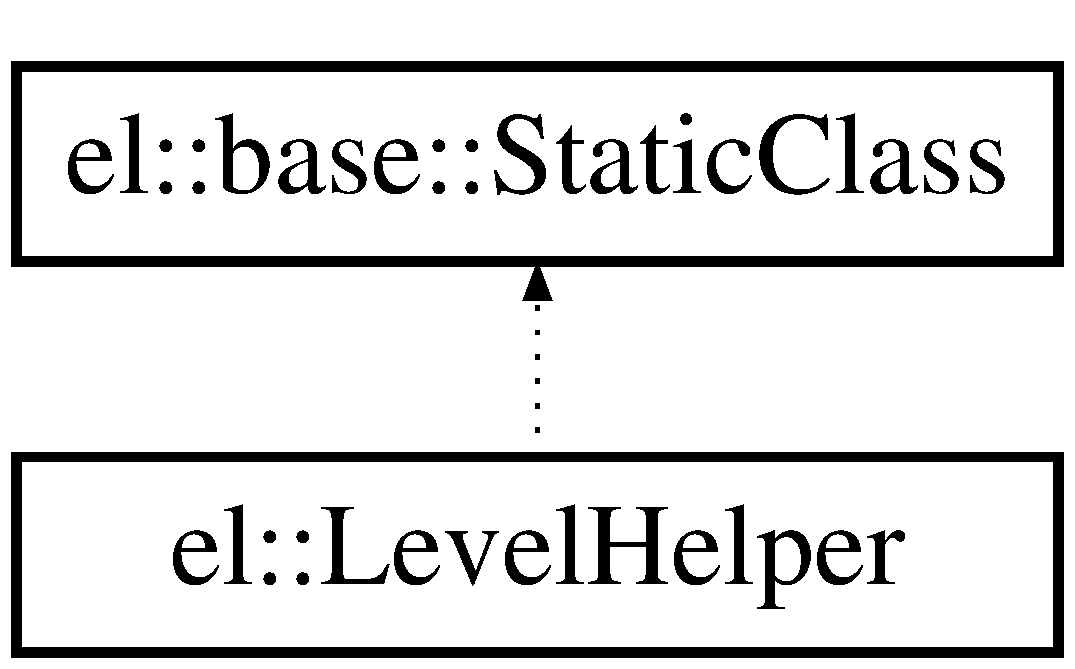
\includegraphics[height=2.000000cm]{classel_1_1LevelHelper}
\end{center}
\end{figure}
\subsection*{Static Public Member Functions}
\begin{DoxyCompactItemize}
\item 
\hypertarget{classel_1_1LevelHelper_a6576fd7cd6d1d839952145115c6e4b38}{static base\-::type\-::\-Enum\-Type \hyperlink{classel_1_1LevelHelper_a6576fd7cd6d1d839952145115c6e4b38}{cast\-To\-Int} (\hyperlink{namespaceel_ab0ac6091262344c52dd2d3ad099e8e36}{Level} level)}\label{classel_1_1LevelHelper_a6576fd7cd6d1d839952145115c6e4b38}

\begin{DoxyCompactList}\small\item\em Casts level to int, useful for iterating through enum. \end{DoxyCompactList}\item 
\hypertarget{classel_1_1LevelHelper_a1279f27df29a003df5ecc3d0bf4dacbb}{static \hyperlink{namespaceel_ab0ac6091262344c52dd2d3ad099e8e36}{Level} \hyperlink{classel_1_1LevelHelper_a1279f27df29a003df5ecc3d0bf4dacbb}{cast\-From\-Int} (base\-::type\-::\-Enum\-Type l)}\label{classel_1_1LevelHelper_a1279f27df29a003df5ecc3d0bf4dacbb}

\begin{DoxyCompactList}\small\item\em Casts int(ushort) to level, useful for iterating through enum. \end{DoxyCompactList}\item 
static const char $\ast$ \hyperlink{classel_1_1LevelHelper_a53b3e226a09af6e87c2072c115b3ba1a}{convert\-To\-String} (\hyperlink{namespaceel_ab0ac6091262344c52dd2d3ad099e8e36}{Level} level)
\begin{DoxyCompactList}\small\item\em Converts level to associated const char$\ast$. \end{DoxyCompactList}\item 
static \hyperlink{namespaceel_ab0ac6091262344c52dd2d3ad099e8e36}{Level} \hyperlink{classel_1_1LevelHelper_a4ff401c62931609c849d580fb6ad2028}{convert\-From\-String} (const char $\ast$level\-Str)
\begin{DoxyCompactList}\small\item\em Converts from level\-Str to Level. \end{DoxyCompactList}\item 
static void \hyperlink{classel_1_1LevelHelper_a94449b79778145f4c58fd1da6bcaf45d}{for\-Each\-Level} (base\-::type\-::\-Enum\-Type $\ast$start\-Index, const std\-::function$<$ bool(void)$>$ \&fn)
\begin{DoxyCompactList}\small\item\em Applies specified function to each level starting from start\-Index. \end{DoxyCompactList}\end{DoxyCompactItemize}
\subsection*{Static Public Attributes}
\begin{DoxyCompactItemize}
\item 
\hypertarget{classel_1_1LevelHelper_a3ecfe43d5b242e9946bad7f61ea4d89d}{static const base\-::type\-::\-Enum\-Type \hyperlink{classel_1_1LevelHelper_a3ecfe43d5b242e9946bad7f61ea4d89d}{k\-Min\-Valid} = static\-\_\-cast$<$base\-::type\-::\-Enum\-Type$>$(\hyperlink{namespaceel_ab0ac6091262344c52dd2d3ad099e8e36add4ec0ac4e58f7c32a01244ae91150b1}{Level\-::\-Trace})}\label{classel_1_1LevelHelper_a3ecfe43d5b242e9946bad7f61ea4d89d}

\begin{DoxyCompactList}\small\item\em Represents minimum valid level. Useful when iterating through enum. \end{DoxyCompactList}\item 
\hypertarget{classel_1_1LevelHelper_aa06e80c65db5c336c4aad25872cf9a48}{static const base\-::type\-::\-Enum\-Type \hyperlink{classel_1_1LevelHelper_aa06e80c65db5c336c4aad25872cf9a48}{k\-Max\-Valid} = static\-\_\-cast$<$base\-::type\-::\-Enum\-Type$>$(\hyperlink{namespaceel_ab0ac6091262344c52dd2d3ad099e8e36a4059b0251f66a18cb56f544728796875}{Level\-::\-Info})}\label{classel_1_1LevelHelper_aa06e80c65db5c336c4aad25872cf9a48}

\begin{DoxyCompactList}\small\item\em Represents maximum valid level. This is used internally and you should not need it. \end{DoxyCompactList}\end{DoxyCompactItemize}


\subsection{Detailed Description}
Static class that contains helper functions for \hyperlink{namespaceel_ab0ac6091262344c52dd2d3ad099e8e36}{el\-::\-Level}. 

\subsection{Member Function Documentation}
\hypertarget{classel_1_1LevelHelper_a4ff401c62931609c849d580fb6ad2028}{\index{el\-::\-Level\-Helper@{el\-::\-Level\-Helper}!convert\-From\-String@{convert\-From\-String}}
\index{convert\-From\-String@{convert\-From\-String}!el::LevelHelper@{el\-::\-Level\-Helper}}
\subsubsection[{convert\-From\-String}]{\setlength{\rightskip}{0pt plus 5cm}static {\bf Level} el\-::\-Level\-Helper\-::convert\-From\-String (
\begin{DoxyParamCaption}
\item[{const char $\ast$}]{level\-Str}
\end{DoxyParamCaption}
)\hspace{0.3cm}{\ttfamily [static]}}}\label{classel_1_1LevelHelper_a4ff401c62931609c849d580fb6ad2028}


Converts from level\-Str to Level. 


\begin{DoxyParams}{Parameters}
{\em level\-Str} & Upper case string based level. Lower case is also valid but providing upper case is recommended. \\
\hline
\end{DoxyParams}
\hypertarget{classel_1_1LevelHelper_a53b3e226a09af6e87c2072c115b3ba1a}{\index{el\-::\-Level\-Helper@{el\-::\-Level\-Helper}!convert\-To\-String@{convert\-To\-String}}
\index{convert\-To\-String@{convert\-To\-String}!el::LevelHelper@{el\-::\-Level\-Helper}}
\subsubsection[{convert\-To\-String}]{\setlength{\rightskip}{0pt plus 5cm}static const char$\ast$ el\-::\-Level\-Helper\-::convert\-To\-String (
\begin{DoxyParamCaption}
\item[{{\bf Level}}]{level}
\end{DoxyParamCaption}
)\hspace{0.3cm}{\ttfamily [static]}}}\label{classel_1_1LevelHelper_a53b3e226a09af6e87c2072c115b3ba1a}


Converts level to associated const char$\ast$. 

\begin{DoxyReturn}{Returns}
Upper case string based level. 
\end{DoxyReturn}
\hypertarget{classel_1_1LevelHelper_a94449b79778145f4c58fd1da6bcaf45d}{\index{el\-::\-Level\-Helper@{el\-::\-Level\-Helper}!for\-Each\-Level@{for\-Each\-Level}}
\index{for\-Each\-Level@{for\-Each\-Level}!el::LevelHelper@{el\-::\-Level\-Helper}}
\subsubsection[{for\-Each\-Level}]{\setlength{\rightskip}{0pt plus 5cm}static void el\-::\-Level\-Helper\-::for\-Each\-Level (
\begin{DoxyParamCaption}
\item[{base\-::type\-::\-Enum\-Type $\ast$}]{start\-Index, }
\item[{const std\-::function$<$ bool(void)$>$ \&}]{fn}
\end{DoxyParamCaption}
)\hspace{0.3cm}{\ttfamily [static]}}}\label{classel_1_1LevelHelper_a94449b79778145f4c58fd1da6bcaf45d}


Applies specified function to each level starting from start\-Index. 


\begin{DoxyParams}{Parameters}
{\em start\-Index} & initial value to start the iteration from. This is passed as pointer and is left-\/shifted so this can be used inside function (fn) to represent current level. \\
\hline
{\em fn} & function to apply with each level. This bool represent whether or not to stop iterating through levels. \\
\hline
\end{DoxyParams}


The documentation for this class was generated from the following file\-:\begin{DoxyCompactItemize}
\item 
/users/disk9/cfse/\-Stage\-\_\-\-Malo/\-C\-P\-A\-C\-S\-Creator\-Lib/\-C\-P\-A\-C\-S\-Creator\-Lib/easylogging++.\-h\end{DoxyCompactItemize}

\hypertarget{classel_1_1LogBuilder}{\section{el\-:\-:Log\-Builder Class Reference}
\label{classel_1_1LogBuilder}\index{el\-::\-Log\-Builder@{el\-::\-Log\-Builder}}
}
Inheritance diagram for el\-:\-:Log\-Builder\-:\begin{figure}[H]
\begin{center}
\leavevmode
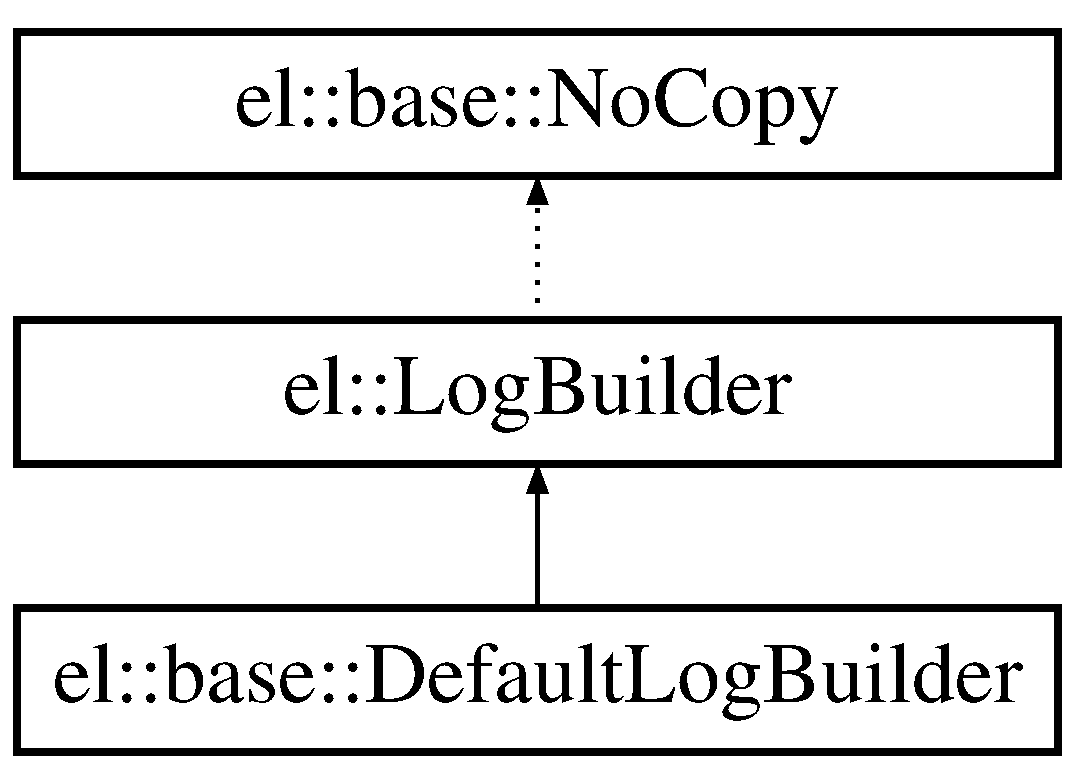
\includegraphics[height=3.000000cm]{classel_1_1LogBuilder}
\end{center}
\end{figure}
\subsection*{Public Member Functions}
\begin{DoxyCompactItemize}
\item 
\hypertarget{classel_1_1LogBuilder_a633b373a3bb9d3e17bdd664aeba4dbc8}{virtual base\-::type\-::string\-\_\-t {\bfseries build} (const \hyperlink{classel_1_1LogMessage}{Log\-Message} $\ast$log\-Message, bool append\-New\-Line) const =0}\label{classel_1_1LogBuilder_a633b373a3bb9d3e17bdd664aeba4dbc8}

\item 
\hypertarget{classel_1_1LogBuilder_a229244f323f25bdbd7725f8bbf983a17}{void {\bfseries convert\-To\-Colored\-Output} (base\-::type\-::string\-\_\-t $\ast$log\-Line, \hyperlink{namespaceel_ab0ac6091262344c52dd2d3ad099e8e36}{Level} level)}\label{classel_1_1LogBuilder_a229244f323f25bdbd7725f8bbf983a17}

\end{DoxyCompactItemize}
\subsection*{Friends}
\begin{DoxyCompactItemize}
\item 
\hypertarget{classel_1_1LogBuilder_a42b1de96d584ae4fecbfc2b9aff95052}{class {\bfseries el\-::base\-::\-Default\-Log\-Dispatch\-Callback}}\label{classel_1_1LogBuilder_a42b1de96d584ae4fecbfc2b9aff95052}

\end{DoxyCompactItemize}


The documentation for this class was generated from the following file\-:\begin{DoxyCompactItemize}
\item 
/users/disk9/cfse/\-Stage\-\_\-\-Malo/\-C\-P\-A\-C\-S\-Creator\-Lib/\-C\-P\-A\-C\-S\-Creator\-Lib/easylogging++.\-h\end{DoxyCompactItemize}

\hypertarget{classel_1_1LogDispatchCallback}{\section{el\-:\-:Log\-Dispatch\-Callback Class Reference}
\label{classel_1_1LogDispatchCallback}\index{el\-::\-Log\-Dispatch\-Callback@{el\-::\-Log\-Dispatch\-Callback}}
}
Inheritance diagram for el\-:\-:Log\-Dispatch\-Callback\-:\begin{figure}[H]
\begin{center}
\leavevmode
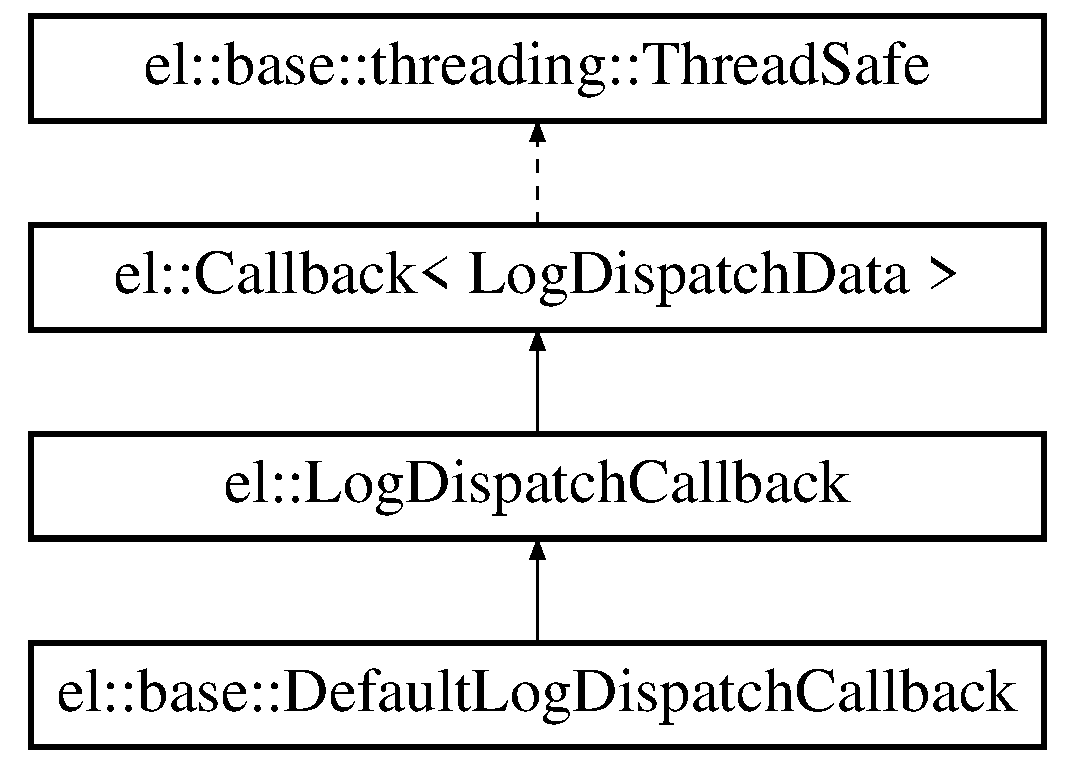
\includegraphics[height=4.000000cm]{classel_1_1LogDispatchCallback}
\end{center}
\end{figure}
\subsection*{Protected Member Functions}
\begin{DoxyCompactItemize}
\item 
\hypertarget{classel_1_1LogDispatchCallback_a7f1af862ca86db91ce282fb252aff6c4}{virtual void {\bfseries handle} (const \hyperlink{classel_1_1LogDispatchData}{Log\-Dispatch\-Data} $\ast$data)}\label{classel_1_1LogDispatchCallback_a7f1af862ca86db91ce282fb252aff6c4}

\item 
\hypertarget{classel_1_1LogDispatchCallback_ab684f5dee1dcced92f61a431acb7d3fb}{\hyperlink{classel_1_1base_1_1threading_1_1internal_1_1NoMutex}{base\-::threading\-::\-Mutex} \& {\bfseries file\-Handle} (const \hyperlink{classel_1_1LogDispatchData}{Log\-Dispatch\-Data} $\ast$data)}\label{classel_1_1LogDispatchCallback_ab684f5dee1dcced92f61a431acb7d3fb}

\end{DoxyCompactItemize}
\subsection*{Friends}
\begin{DoxyCompactItemize}
\item 
\hypertarget{classel_1_1LogDispatchCallback_a84d22f9ad5b796e49ff5f15a8c32773d}{class {\bfseries base\-::\-Log\-Dispatcher}}\label{classel_1_1LogDispatchCallback_a84d22f9ad5b796e49ff5f15a8c32773d}

\end{DoxyCompactItemize}
\subsection*{Additional Inherited Members}


The documentation for this class was generated from the following file\-:\begin{DoxyCompactItemize}
\item 
/users/disk9/cfse/\-Stage\-\_\-\-Malo/\-C\-P\-A\-C\-S\-Creator\-Lib/\-C\-P\-A\-C\-S\-Creator\-Lib/easylogging++.\-h\end{DoxyCompactItemize}

\hypertarget{classel_1_1LogDispatchData}{\section{el\-:\-:Log\-Dispatch\-Data Class Reference}
\label{classel_1_1LogDispatchData}\index{el\-::\-Log\-Dispatch\-Data@{el\-::\-Log\-Dispatch\-Data}}
}
\subsection*{Public Member Functions}
\begin{DoxyCompactItemize}
\item 
\hypertarget{classel_1_1LogDispatchData_ad52d4ddc330b6260bf10e9879a653829}{const \hyperlink{classel_1_1LogMessage}{Log\-Message} $\ast$ {\bfseries log\-Message} (void) const }\label{classel_1_1LogDispatchData_ad52d4ddc330b6260bf10e9879a653829}

\item 
\hypertarget{classel_1_1LogDispatchData_aee0808c660aa39b34ee69850a2c74c09}{\hyperlink{namespaceel_1_1base_a3aa2563d38e47388ba242a1694fc2839}{base\-::\-Dispatch\-Action} {\bfseries dispatch\-Action} (void) const }\label{classel_1_1LogDispatchData_aee0808c660aa39b34ee69850a2c74c09}

\item 
\hypertarget{classel_1_1LogDispatchData_a09fcf704874e1f0a9d9061fafdaa0ce8}{void {\bfseries set\-Log\-Message} (\hyperlink{classel_1_1LogMessage}{Log\-Message} $\ast$log\-Message)}\label{classel_1_1LogDispatchData_a09fcf704874e1f0a9d9061fafdaa0ce8}

\item 
\hypertarget{classel_1_1LogDispatchData_ae85d1d70f93b81ec57f058cf4bda27d4}{void {\bfseries set\-Dispatch\-Action} (\hyperlink{namespaceel_1_1base_a3aa2563d38e47388ba242a1694fc2839}{base\-::\-Dispatch\-Action} dispatch\-Action)}\label{classel_1_1LogDispatchData_ae85d1d70f93b81ec57f058cf4bda27d4}

\end{DoxyCompactItemize}
\subsection*{Friends}
\begin{DoxyCompactItemize}
\item 
\hypertarget{classel_1_1LogDispatchData_a84d22f9ad5b796e49ff5f15a8c32773d}{class {\bfseries base\-::\-Log\-Dispatcher}}\label{classel_1_1LogDispatchData_a84d22f9ad5b796e49ff5f15a8c32773d}

\end{DoxyCompactItemize}


The documentation for this class was generated from the following file\-:\begin{DoxyCompactItemize}
\item 
/users/disk9/cfse/\-Stage\-\_\-\-Malo/\-C\-P\-A\-C\-S\-Creator\-Lib/\-C\-P\-A\-C\-S\-Creator\-Lib/easylogging++.\-h\end{DoxyCompactItemize}

\hypertarget{classel_1_1base_1_1LogDispatcher}{\section{el\-:\-:base\-:\-:Log\-Dispatcher Class Reference}
\label{classel_1_1base_1_1LogDispatcher}\index{el\-::base\-::\-Log\-Dispatcher@{el\-::base\-::\-Log\-Dispatcher}}
}


Dispatches log messages.  




{\ttfamily \#include $<$easylogging++.\-h$>$}

Inheritance diagram for el\-:\-:base\-:\-:Log\-Dispatcher\-:\begin{figure}[H]
\begin{center}
\leavevmode
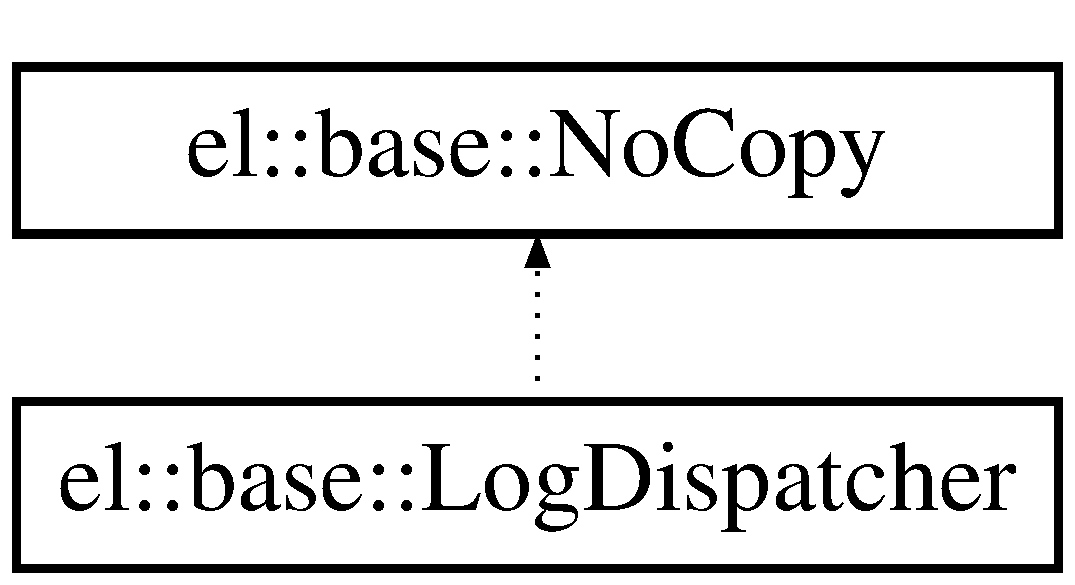
\includegraphics[height=2.000000cm]{classel_1_1base_1_1LogDispatcher}
\end{center}
\end{figure}
\subsection*{Public Member Functions}
\begin{DoxyCompactItemize}
\item 
\hypertarget{classel_1_1base_1_1LogDispatcher_a21a9210cbaa93907f2e5519995dd26e2}{{\bfseries Log\-Dispatcher} (bool proceed, \hyperlink{classel_1_1LogMessage}{Log\-Message} $\ast$log\-Message, \hyperlink{namespaceel_1_1base_a3aa2563d38e47388ba242a1694fc2839}{base\-::\-Dispatch\-Action} dispatch\-Action)}\label{classel_1_1base_1_1LogDispatcher_a21a9210cbaa93907f2e5519995dd26e2}

\item 
\hypertarget{classel_1_1base_1_1LogDispatcher_a88d4a644364bb454136c85338f05da7a}{void {\bfseries dispatch} (void)}\label{classel_1_1base_1_1LogDispatcher_a88d4a644364bb454136c85338f05da7a}

\end{DoxyCompactItemize}


\subsection{Detailed Description}
Dispatches log messages. 

The documentation for this class was generated from the following file\-:\begin{DoxyCompactItemize}
\item 
/users/disk9/cfse/\-Stage\-\_\-\-Malo/\-C\-P\-A\-C\-S\-Creator\-Lib/\-C\-P\-A\-C\-S\-Creator\-Lib/easylogging++.\-h\end{DoxyCompactItemize}

\hypertarget{classel_1_1base_1_1LogFormat}{\section{el\-:\-:base\-:\-:Log\-Format Class Reference}
\label{classel_1_1base_1_1LogFormat}\index{el\-::base\-::\-Log\-Format@{el\-::base\-::\-Log\-Format}}
}


Represents log format containing flags and date format. This is used internally to start initial log.  




{\ttfamily \#include $<$easylogging++.\-h$>$}

Inheritance diagram for el\-:\-:base\-:\-:Log\-Format\-:\begin{figure}[H]
\begin{center}
\leavevmode
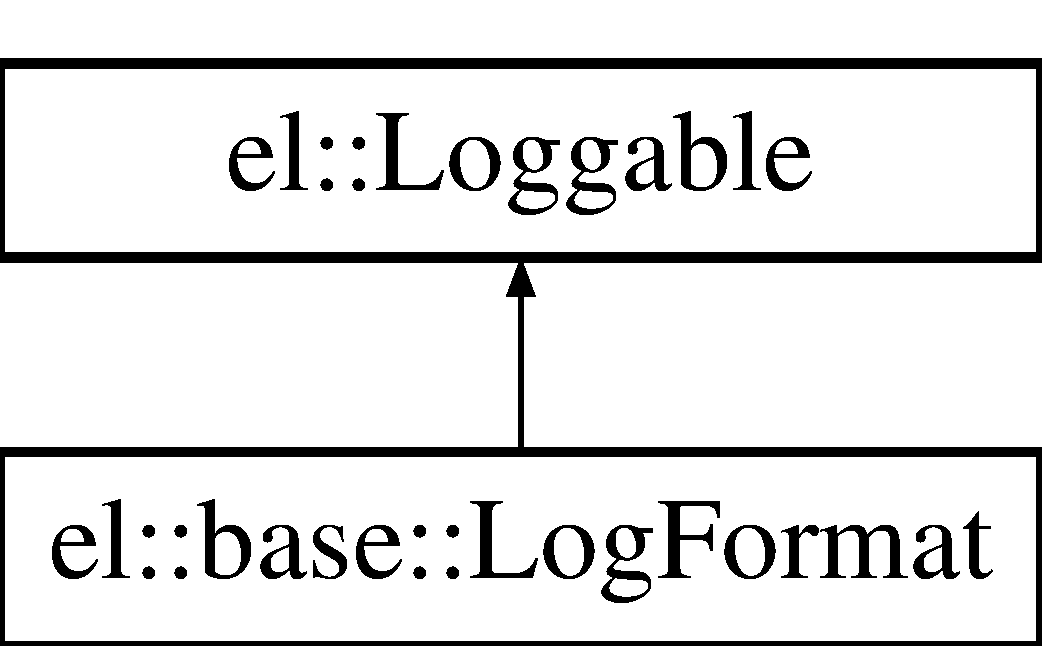
\includegraphics[height=2.000000cm]{classel_1_1base_1_1LogFormat}
\end{center}
\end{figure}
\subsection*{Public Member Functions}
\begin{DoxyCompactItemize}
\item 
\hypertarget{classel_1_1base_1_1LogFormat_a746a49231f1b046803dd2144ae2a2c76}{{\bfseries Log\-Format} (\hyperlink{namespaceel_ab0ac6091262344c52dd2d3ad099e8e36}{Level} level, const base\-::type\-::string\-\_\-t \&format)}\label{classel_1_1base_1_1LogFormat_a746a49231f1b046803dd2144ae2a2c76}

\item 
\hypertarget{classel_1_1base_1_1LogFormat_a8cc88ab095024bcfb90dd3ad7208f2ef}{{\bfseries Log\-Format} (const \hyperlink{classel_1_1base_1_1LogFormat}{Log\-Format} \&log\-Format)}\label{classel_1_1base_1_1LogFormat_a8cc88ab095024bcfb90dd3ad7208f2ef}

\item 
\hypertarget{classel_1_1base_1_1LogFormat_a697d52d55c6b6c6b8e6d5ceb37d66c19}{{\bfseries Log\-Format} (\hyperlink{classel_1_1base_1_1LogFormat}{Log\-Format} \&\&log\-Format)}\label{classel_1_1base_1_1LogFormat_a697d52d55c6b6c6b8e6d5ceb37d66c19}

\item 
\hypertarget{classel_1_1base_1_1LogFormat_a3c81e5976c3f3a8cb428eeeb3f188ac2}{\hyperlink{classel_1_1base_1_1LogFormat}{Log\-Format} \& {\bfseries operator=} (const \hyperlink{classel_1_1base_1_1LogFormat}{Log\-Format} \&log\-Format)}\label{classel_1_1base_1_1LogFormat_a3c81e5976c3f3a8cb428eeeb3f188ac2}

\item 
\hypertarget{classel_1_1base_1_1LogFormat_a31e85c6f74da6fe36d156a89a6c7fb91}{bool {\bfseries operator==} (const \hyperlink{classel_1_1base_1_1LogFormat}{Log\-Format} \&other)}\label{classel_1_1base_1_1LogFormat_a31e85c6f74da6fe36d156a89a6c7fb91}

\item 
void \hyperlink{classel_1_1base_1_1LogFormat_ab7c1b15cfdad24cfbc6dbced8b9d66eb}{parse\-From\-Format} (const base\-::type\-::string\-\_\-t \&user\-Format)
\begin{DoxyCompactList}\small\item\em Updates format to be used while logging. \end{DoxyCompactList}\item 
\hypertarget{classel_1_1base_1_1LogFormat_a6c5d17ad378ccb6e53beb2d48143fecb}{\hyperlink{namespaceel_ab0ac6091262344c52dd2d3ad099e8e36}{Level} {\bfseries level} (void) const }\label{classel_1_1base_1_1LogFormat_a6c5d17ad378ccb6e53beb2d48143fecb}

\item 
\hypertarget{classel_1_1base_1_1LogFormat_a9ca6ecd5b9342653493670d5a4e230cd}{const base\-::type\-::string\-\_\-t \& {\bfseries user\-Format} (void) const }\label{classel_1_1base_1_1LogFormat_a9ca6ecd5b9342653493670d5a4e230cd}

\item 
\hypertarget{classel_1_1base_1_1LogFormat_ac19602b3153daa9a76b56d3f4ff3beaa}{const base\-::type\-::string\-\_\-t \& {\bfseries format} (void) const }\label{classel_1_1base_1_1LogFormat_ac19602b3153daa9a76b56d3f4ff3beaa}

\item 
\hypertarget{classel_1_1base_1_1LogFormat_aa06b2643592f8a441d93cde673640262}{const std\-::string \& {\bfseries date\-Time\-Format} (void) const }\label{classel_1_1base_1_1LogFormat_aa06b2643592f8a441d93cde673640262}

\item 
\hypertarget{classel_1_1base_1_1LogFormat_a3ecf5f8df9b9e090784e19ad76046c49}{base\-::type\-::\-Enum\-Type {\bfseries flags} (void) const }\label{classel_1_1base_1_1LogFormat_a3ecf5f8df9b9e090784e19ad76046c49}

\item 
\hypertarget{classel_1_1base_1_1LogFormat_ae3634f9d90f7339d99eec8512b46c734}{bool {\bfseries has\-Flag} (\hyperlink{namespaceel_1_1base_a28939c5a884e67fcf12259f4b8848e00}{base\-::\-Format\-Flags} flag) const }\label{classel_1_1base_1_1LogFormat_ae3634f9d90f7339d99eec8512b46c734}

\item 
\hypertarget{classel_1_1base_1_1LogFormat_a0cae595d1a367538243feb1be1555d2e}{virtual void {\bfseries log} (el\-::base\-::type\-::ostream\-\_\-t \&os) const }\label{classel_1_1base_1_1LogFormat_a0cae595d1a367538243feb1be1555d2e}

\end{DoxyCompactItemize}
\subsection*{Protected Member Functions}
\begin{DoxyCompactItemize}
\item 
virtual void \hyperlink{classel_1_1base_1_1LogFormat_a3146651eadd6b1164bde74e5b273ec94}{update\-Date\-Format} (std\-::size\-\_\-t index, base\-::type\-::string\-\_\-t \&curr\-Format) E\-L\-P\-P\-\_\-\-F\-I\-N\-A\-L
\begin{DoxyCompactList}\small\item\em Updates date time format if available in curr\-Format. \end{DoxyCompactList}\item 
\hypertarget{classel_1_1base_1_1LogFormat_afee2335cce2b627dfd7f918d5a2b85f3}{virtual void \hyperlink{classel_1_1base_1_1LogFormat_afee2335cce2b627dfd7f918d5a2b85f3}{update\-Format\-Spec} (void) E\-L\-P\-P\-\_\-\-F\-I\-N\-A\-L}\label{classel_1_1base_1_1LogFormat_afee2335cce2b627dfd7f918d5a2b85f3}

\begin{DoxyCompactList}\small\item\em Updates level from format. This is so that we dont have to do it at log-\/writing-\/time. It uses m\-\_\-format and m\-\_\-level. \end{DoxyCompactList}\item 
\hypertarget{classel_1_1base_1_1LogFormat_ae55910f533a6eb3b41eb75b131e522bf}{void {\bfseries add\-Flag} (\hyperlink{namespaceel_1_1base_a28939c5a884e67fcf12259f4b8848e00}{base\-::\-Format\-Flags} flag)}\label{classel_1_1base_1_1LogFormat_ae55910f533a6eb3b41eb75b131e522bf}

\end{DoxyCompactItemize}
\subsection*{Friends}
\begin{DoxyCompactItemize}
\item 
\hypertarget{classel_1_1base_1_1LogFormat_aa78553f3fecc0d9551408dfd7aa7f737}{class {\bfseries el\-::\-Logger}}\label{classel_1_1base_1_1LogFormat_aa78553f3fecc0d9551408dfd7aa7f737}

\end{DoxyCompactItemize}


\subsection{Detailed Description}
Represents log format containing flags and date format. This is used internally to start initial log. 

\subsection{Member Function Documentation}
\hypertarget{classel_1_1base_1_1LogFormat_ab7c1b15cfdad24cfbc6dbced8b9d66eb}{\index{el\-::base\-::\-Log\-Format@{el\-::base\-::\-Log\-Format}!parse\-From\-Format@{parse\-From\-Format}}
\index{parse\-From\-Format@{parse\-From\-Format}!el::base::LogFormat@{el\-::base\-::\-Log\-Format}}
\subsubsection[{parse\-From\-Format}]{\setlength{\rightskip}{0pt plus 5cm}void el\-::base\-::\-Log\-Format\-::parse\-From\-Format (
\begin{DoxyParamCaption}
\item[{const base\-::type\-::string\-\_\-t \&}]{user\-Format}
\end{DoxyParamCaption}
)}}\label{classel_1_1base_1_1LogFormat_ab7c1b15cfdad24cfbc6dbced8b9d66eb}


Updates format to be used while logging. 


\begin{DoxyParams}{Parameters}
{\em user\-Format} & User provided format \\
\hline
\end{DoxyParams}
\hypertarget{classel_1_1base_1_1LogFormat_a3146651eadd6b1164bde74e5b273ec94}{\index{el\-::base\-::\-Log\-Format@{el\-::base\-::\-Log\-Format}!update\-Date\-Format@{update\-Date\-Format}}
\index{update\-Date\-Format@{update\-Date\-Format}!el::base::LogFormat@{el\-::base\-::\-Log\-Format}}
\subsubsection[{update\-Date\-Format}]{\setlength{\rightskip}{0pt plus 5cm}virtual void el\-::base\-::\-Log\-Format\-::update\-Date\-Format (
\begin{DoxyParamCaption}
\item[{std\-::size\-\_\-t}]{index, }
\item[{base\-::type\-::string\-\_\-t \&}]{curr\-Format}
\end{DoxyParamCaption}
)\hspace{0.3cm}{\ttfamily [protected]}, {\ttfamily [virtual]}}}\label{classel_1_1base_1_1LogFormat_a3146651eadd6b1164bde74e5b273ec94}


Updates date time format if available in curr\-Format. 


\begin{DoxyParams}[1]{Parameters}
 & {\em index} & Index where datetime, date or time was found \\
\hline
\mbox{\tt in,out}  & {\em curr\-Format} & current format that is being used to format \\
\hline
\end{DoxyParams}


The documentation for this class was generated from the following file\-:\begin{DoxyCompactItemize}
\item 
/users/disk9/cfse/\-Stage\-\_\-\-Malo/\-C\-P\-A\-C\-S\-Creator\-Lib/\-C\-P\-A\-C\-S\-Creator\-Lib/easylogging++.\-h\end{DoxyCompactItemize}

\hypertarget{classel_1_1Loggable}{\section{el\-:\-:Loggable Class Reference}
\label{classel_1_1Loggable}\index{el\-::\-Loggable@{el\-::\-Loggable}}
}


Base of Easylogging++ friendly class.  




{\ttfamily \#include $<$easylogging++.\-h$>$}

Inheritance diagram for el\-:\-:Loggable\-:\begin{figure}[H]
\begin{center}
\leavevmode
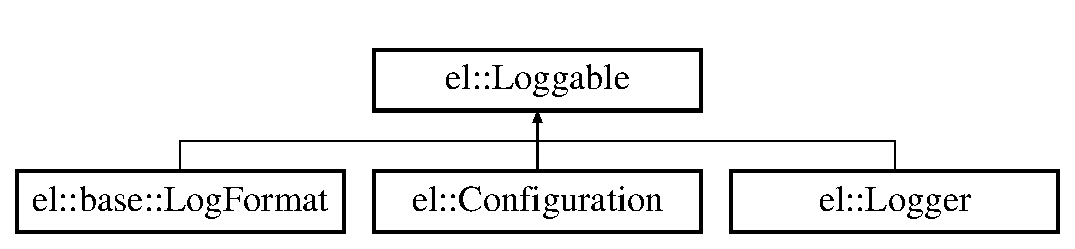
\includegraphics[height=2.000000cm]{classel_1_1Loggable}
\end{center}
\end{figure}
\subsection*{Public Member Functions}
\begin{DoxyCompactItemize}
\item 
\hypertarget{classel_1_1Loggable_ad8a2e0ebc11e4bd00ef49fc67db3d59e}{virtual void {\bfseries log} (el\-::base\-::type\-::ostream\-\_\-t \&) const =0}\label{classel_1_1Loggable_ad8a2e0ebc11e4bd00ef49fc67db3d59e}

\end{DoxyCompactItemize}
\subsection*{Friends}
\begin{DoxyCompactItemize}
\item 
\hypertarget{classel_1_1Loggable_a00722a386f498be3ebece2e266fb0f05}{el\-::base\-::type\-::ostream\-\_\-t \& {\bfseries operator$<$$<$} (el\-::base\-::type\-::ostream\-\_\-t \&os, const \hyperlink{classel_1_1Loggable}{Loggable} \&loggable)}\label{classel_1_1Loggable_a00722a386f498be3ebece2e266fb0f05}

\end{DoxyCompactItemize}


\subsection{Detailed Description}
Base of Easylogging++ friendly class. 

After inheriting this class publicly, implement pure-\/virtual function {\ttfamily void log(std\-::ostream\&) const} 

The documentation for this class was generated from the following file\-:\begin{DoxyCompactItemize}
\item 
/users/disk9/cfse/\-Stage\-\_\-\-Malo/\-C\-P\-A\-C\-S\-Creator\-Lib/\-C\-P\-A\-C\-S\-Creator\-Lib/easylogging++.\-h\end{DoxyCompactItemize}

\hypertarget{classel_1_1Logger}{\section{el\-:\-:Logger Class Reference}
\label{classel_1_1Logger}\index{el\-::\-Logger@{el\-::\-Logger}}
}


Represents a logger holding I\-D and configurations we need to write logs.  




{\ttfamily \#include $<$easylogging++.\-h$>$}

Inheritance diagram for el\-:\-:Logger\-:\begin{figure}[H]
\begin{center}
\leavevmode
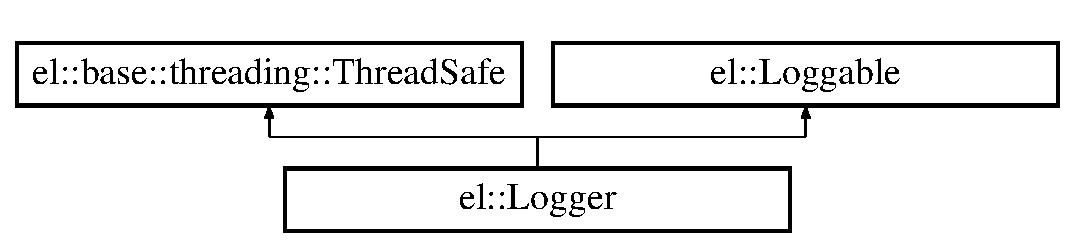
\includegraphics[height=2.000000cm]{classel_1_1Logger}
\end{center}
\end{figure}
\subsection*{Public Member Functions}
\begin{DoxyCompactItemize}
\item 
\hypertarget{classel_1_1Logger_a59b1c5a0f8c5c670e59d2f69f9e39fbb}{{\bfseries Logger} (const std\-::string \&id, base\-::\-Log\-Streams\-Reference\-Map $\ast$log\-Streams\-Reference)}\label{classel_1_1Logger_a59b1c5a0f8c5c670e59d2f69f9e39fbb}

\item 
\hypertarget{classel_1_1Logger_a43abea8865d7316f05c8a676a8c04896}{{\bfseries Logger} (const std\-::string \&id, const \hyperlink{classel_1_1Configurations}{Configurations} \&configurations, base\-::\-Log\-Streams\-Reference\-Map $\ast$log\-Streams\-Reference)}\label{classel_1_1Logger_a43abea8865d7316f05c8a676a8c04896}

\item 
\hypertarget{classel_1_1Logger_a984de07936a8c783e91496dfa6df69ea}{{\bfseries Logger} (const \hyperlink{classel_1_1Logger}{Logger} \&logger)}\label{classel_1_1Logger_a984de07936a8c783e91496dfa6df69ea}

\item 
\hypertarget{classel_1_1Logger_a2bfb4ed37f3281a701f20fb21a4cac62}{\hyperlink{classel_1_1Logger}{Logger} \& {\bfseries operator=} (const \hyperlink{classel_1_1Logger}{Logger} \&logger)}\label{classel_1_1Logger_a2bfb4ed37f3281a701f20fb21a4cac62}

\item 
\hypertarget{classel_1_1Logger_a12e1e5f6f91bad8d6a71c3918f09b672}{virtual void {\bfseries log} (el\-::base\-::type\-::ostream\-\_\-t \&os) const }\label{classel_1_1Logger_a12e1e5f6f91bad8d6a71c3918f09b672}

\item 
\hypertarget{classel_1_1Logger_ad9db621dbf8977bf814dc7baea8dcee4}{void \hyperlink{classel_1_1Logger_ad9db621dbf8977bf814dc7baea8dcee4}{configure} (const \hyperlink{classel_1_1Configurations}{Configurations} \&configurations)}\label{classel_1_1Logger_ad9db621dbf8977bf814dc7baea8dcee4}

\begin{DoxyCompactList}\small\item\em Configures the logger using specified configurations. \end{DoxyCompactList}\item 
\hypertarget{classel_1_1Logger_adfd57ab27fb398cc980a3edfab92927e}{void \hyperlink{classel_1_1Logger_adfd57ab27fb398cc980a3edfab92927e}{reconfigure} (void)}\label{classel_1_1Logger_adfd57ab27fb398cc980a3edfab92927e}

\begin{DoxyCompactList}\small\item\em Reconfigures logger using existing configurations. \end{DoxyCompactList}\item 
\hypertarget{classel_1_1Logger_ae51a621df3c835f51f450134ba66f8ac}{const std\-::string \& {\bfseries id} (void) const }\label{classel_1_1Logger_ae51a621df3c835f51f450134ba66f8ac}

\item 
\hypertarget{classel_1_1Logger_a9e56e468bccd7b52281e7bbc75892431}{const std\-::string \& {\bfseries parent\-Application\-Name} (void) const }\label{classel_1_1Logger_a9e56e468bccd7b52281e7bbc75892431}

\item 
\hypertarget{classel_1_1Logger_a6890af8910adba26b01ef029429c4f15}{void {\bfseries set\-Parent\-Application\-Name} (const std\-::string \&parent\-Application\-Name)}\label{classel_1_1Logger_a6890af8910adba26b01ef029429c4f15}

\item 
\hypertarget{classel_1_1Logger_aeb57aeaddbb3dcd0cb96114019817142}{\hyperlink{classel_1_1Configurations}{Configurations} $\ast$ {\bfseries configurations} (void)}\label{classel_1_1Logger_aeb57aeaddbb3dcd0cb96114019817142}

\item 
\hypertarget{classel_1_1Logger_ac1d34e77892ea506b011d5279b6b139d}{\hyperlink{classel_1_1base_1_1TypedConfigurations}{base\-::\-Typed\-Configurations} $\ast$ {\bfseries typed\-Configurations} (void)}\label{classel_1_1Logger_ac1d34e77892ea506b011d5279b6b139d}

\item 
\hypertarget{classel_1_1Logger_a9a89d454008b1ee1a197eec4b92ce22a}{void \hyperlink{classel_1_1Logger_a9a89d454008b1ee1a197eec4b92ce22a}{flush} (void)}\label{classel_1_1Logger_a9a89d454008b1ee1a197eec4b92ce22a}

\begin{DoxyCompactList}\small\item\em Flushes logger to sync all log files for all levels. \end{DoxyCompactList}\item 
\hypertarget{classel_1_1Logger_a83c85278ebeeef6a24cc112e56c344dd}{void {\bfseries flush} (\hyperlink{namespaceel_ab0ac6091262344c52dd2d3ad099e8e36}{Level} level, base\-::type\-::fstream\-\_\-t $\ast$fs)}\label{classel_1_1Logger_a83c85278ebeeef6a24cc112e56c344dd}

\item 
\hypertarget{classel_1_1Logger_abdf56c00388c71d1cbaa7e2df4449202}{bool {\bfseries is\-Flush\-Needed} (\hyperlink{namespaceel_ab0ac6091262344c52dd2d3ad099e8e36}{Level} level)}\label{classel_1_1Logger_abdf56c00388c71d1cbaa7e2df4449202}

\item 
\hypertarget{classel_1_1Logger_aead5b130c5141d2024740b03ab4b45d7}{\hyperlink{classel_1_1LogBuilder}{Log\-Builder} $\ast$ {\bfseries log\-Builder} (void) const }\label{classel_1_1Logger_aead5b130c5141d2024740b03ab4b45d7}

\item 
\hypertarget{classel_1_1Logger_a737340322cc9d9d20febd7131c1e262f}{void {\bfseries set\-Log\-Builder} (const Log\-Builder\-Ptr \&log\-Builder)}\label{classel_1_1Logger_a737340322cc9d9d20febd7131c1e262f}

\item 
\hypertarget{classel_1_1Logger_a5abaca24ac28bfd4806bea32be193435}{bool {\bfseries enabled} (\hyperlink{namespaceel_ab0ac6091262344c52dd2d3ad099e8e36}{Level} level) const }\label{classel_1_1Logger_a5abaca24ac28bfd4806bea32be193435}

\end{DoxyCompactItemize}
\subsection*{Static Public Member Functions}
\begin{DoxyCompactItemize}
\item 
\hypertarget{classel_1_1Logger_af6cf4f266ceb65da9563afd3706f26d6}{static bool {\bfseries is\-Valid\-Id} (const std\-::string \&id)}\label{classel_1_1Logger_af6cf4f266ceb65da9563afd3706f26d6}

\end{DoxyCompactItemize}
\subsection*{Friends}
\begin{DoxyCompactItemize}
\item 
\hypertarget{classel_1_1Logger_a22965b691242a9f61d443ba03fce3e35}{class {\bfseries el\-::\-Log\-Message}}\label{classel_1_1Logger_a22965b691242a9f61d443ba03fce3e35}

\item 
\hypertarget{classel_1_1Logger_a6efe246b312d02731fb0e1d120c0331d}{class {\bfseries el\-::\-Loggers}}\label{classel_1_1Logger_a6efe246b312d02731fb0e1d120c0331d}

\item 
\hypertarget{classel_1_1Logger_a2fb8a2c02cbf86247f093c118bed877a}{class {\bfseries el\-::\-Helpers}}\label{classel_1_1Logger_a2fb8a2c02cbf86247f093c118bed877a}

\item 
\hypertarget{classel_1_1Logger_a574ecee25e8d578f76060a95a2fe7c9e}{class {\bfseries el\-::base\-::\-Registered\-Loggers}}\label{classel_1_1Logger_a574ecee25e8d578f76060a95a2fe7c9e}

\item 
\hypertarget{classel_1_1Logger_a42b1de96d584ae4fecbfc2b9aff95052}{class {\bfseries el\-::base\-::\-Default\-Log\-Dispatch\-Callback}}\label{classel_1_1Logger_a42b1de96d584ae4fecbfc2b9aff95052}

\item 
\hypertarget{classel_1_1Logger_a81bbf6fe31fab133d182efa8367304f1}{class {\bfseries el\-::base\-::\-Message\-Builder}}\label{classel_1_1Logger_a81bbf6fe31fab133d182efa8367304f1}

\item 
\hypertarget{classel_1_1Logger_a7a728edbb2761d151832daa74d5b2736}{class {\bfseries el\-::base\-::\-Writer}}\label{classel_1_1Logger_a7a728edbb2761d151832daa74d5b2736}

\item 
\hypertarget{classel_1_1Logger_a2a368b9be1b8d6a29d4bb92a11807f39}{class {\bfseries el\-::base\-::\-P\-Error\-Writer}}\label{classel_1_1Logger_a2a368b9be1b8d6a29d4bb92a11807f39}

\item 
\hypertarget{classel_1_1Logger_acc1efd1b8a3fc5e0028dab98b02e550a}{class {\bfseries el\-::base\-::\-Storage}}\label{classel_1_1Logger_acc1efd1b8a3fc5e0028dab98b02e550a}

\item 
\hypertarget{classel_1_1Logger_a6a4d7851e1984800be3c230f06a79528}{class {\bfseries el\-::base\-::\-Performance\-Tracker}}\label{classel_1_1Logger_a6a4d7851e1984800be3c230f06a79528}

\item 
\hypertarget{classel_1_1Logger_a9b37b28ea1c5f8f862cc89f135711d92}{class {\bfseries el\-::base\-::\-Log\-Dispatcher}}\label{classel_1_1Logger_a9b37b28ea1c5f8f862cc89f135711d92}

\end{DoxyCompactItemize}


\subsection{Detailed Description}
Represents a logger holding I\-D and configurations we need to write logs. 

This class does not write logs itself instead its used by writer to read configuations from. 

The documentation for this class was generated from the following file\-:\begin{DoxyCompactItemize}
\item 
/users/disk9/cfse/\-Stage\-\_\-\-Malo/\-C\-P\-A\-C\-S\-Creator\-Lib/\-C\-P\-A\-C\-S\-Creator\-Lib/easylogging++.\-h\end{DoxyCompactItemize}

\hypertarget{classel_1_1LoggerRegistrationCallback}{\section{el\-:\-:Logger\-Registration\-Callback Class Reference}
\label{classel_1_1LoggerRegistrationCallback}\index{el\-::\-Logger\-Registration\-Callback@{el\-::\-Logger\-Registration\-Callback}}
}
Inheritance diagram for el\-:\-:Logger\-Registration\-Callback\-:\begin{figure}[H]
\begin{center}
\leavevmode
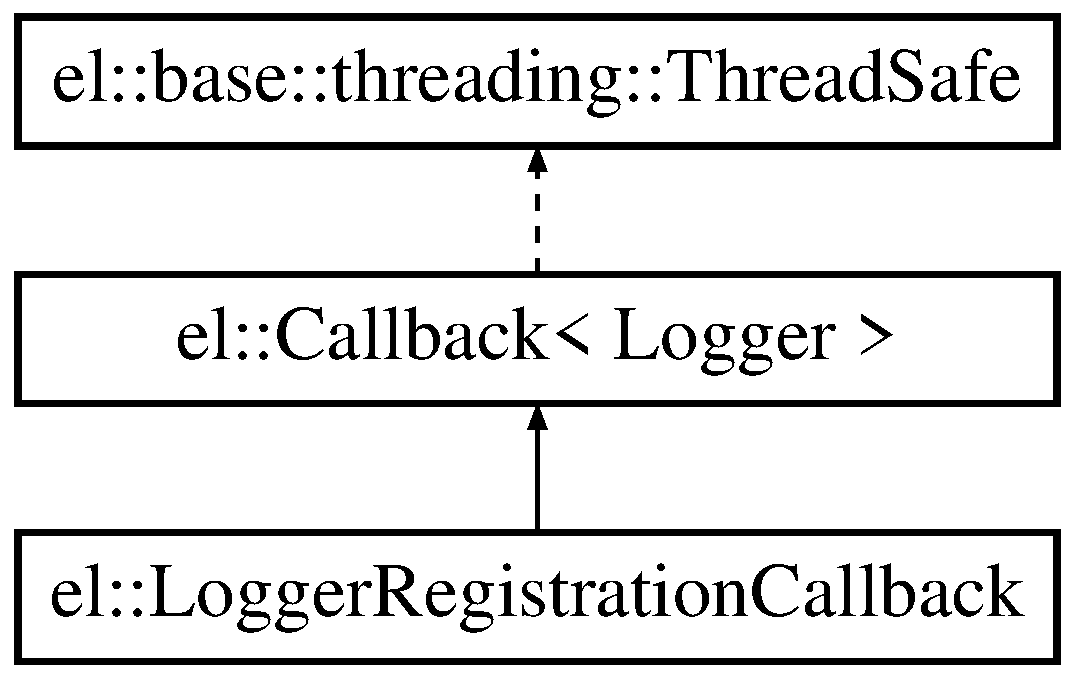
\includegraphics[height=3.000000cm]{classel_1_1LoggerRegistrationCallback}
\end{center}
\end{figure}
\subsection*{Friends}
\begin{DoxyCompactItemize}
\item 
\hypertarget{classel_1_1LoggerRegistrationCallback_a5b2ecdd0901cd8ea80e03a3a6e2a9f17}{class {\bfseries base\-::\-Registered\-Loggers}}\label{classel_1_1LoggerRegistrationCallback_a5b2ecdd0901cd8ea80e03a3a6e2a9f17}

\end{DoxyCompactItemize}
\subsection*{Additional Inherited Members}


The documentation for this class was generated from the following file\-:\begin{DoxyCompactItemize}
\item 
/users/disk9/cfse/\-Stage\-\_\-\-Malo/\-C\-P\-A\-C\-S\-Creator\-Lib/\-C\-P\-A\-C\-S\-Creator\-Lib/easylogging++.\-h\end{DoxyCompactItemize}

\hypertarget{classel_1_1Loggers}{\section{el\-:\-:Loggers Class Reference}
\label{classel_1_1Loggers}\index{el\-::\-Loggers@{el\-::\-Loggers}}
}


Static helpers to deal with loggers and their configurations.  




{\ttfamily \#include $<$easylogging++.\-h$>$}

Inheritance diagram for el\-:\-:Loggers\-:\begin{figure}[H]
\begin{center}
\leavevmode
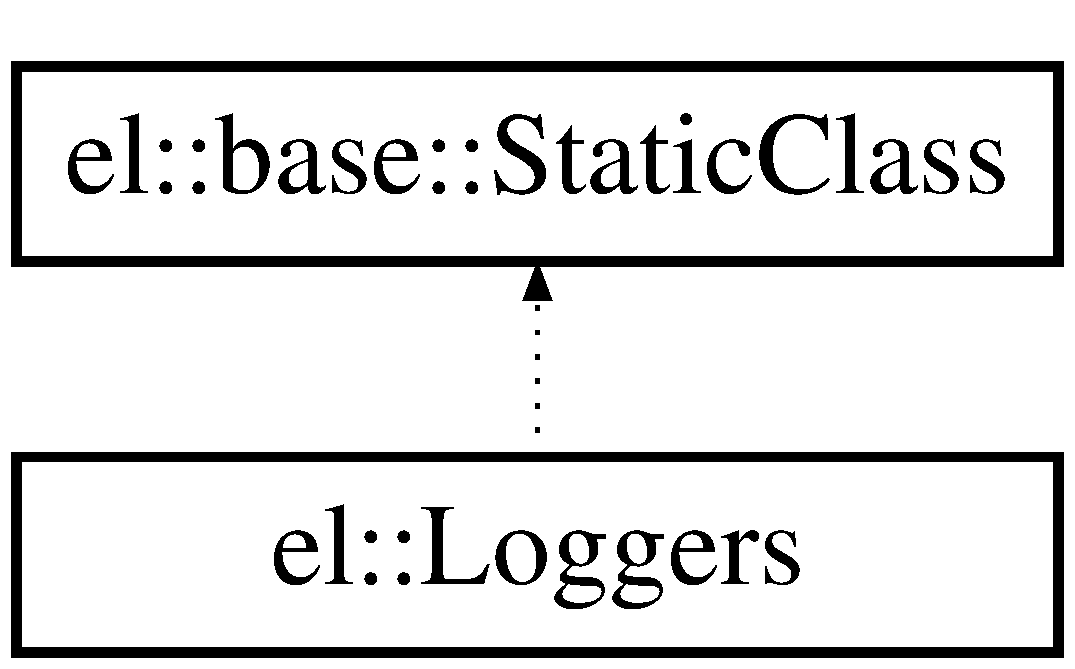
\includegraphics[height=2.000000cm]{classel_1_1Loggers}
\end{center}
\end{figure}
\subsection*{Classes}
\begin{DoxyCompactItemize}
\item 
class \hyperlink{classel_1_1Loggers_1_1ScopedAddFlag}{Scoped\-Add\-Flag}
\begin{DoxyCompactList}\small\item\em Adds flag and removes it when scope goes out. \end{DoxyCompactList}\item 
class \hyperlink{classel_1_1Loggers_1_1ScopedRemoveFlag}{Scoped\-Remove\-Flag}
\begin{DoxyCompactList}\small\item\em Removes flag and add it when scope goes out. \end{DoxyCompactList}\end{DoxyCompactItemize}
\subsection*{Static Public Member Functions}
\begin{DoxyCompactItemize}
\item 
\hypertarget{classel_1_1Loggers_aaebf868c558e3ba1d2e4f073a00f1d4a}{static \hyperlink{classel_1_1Logger}{Logger} $\ast$ \hyperlink{classel_1_1Loggers_aaebf868c558e3ba1d2e4f073a00f1d4a}{get\-Logger} (const std\-::string \&identity, bool register\-If\-Not\-Available=true)}\label{classel_1_1Loggers_aaebf868c558e3ba1d2e4f073a00f1d4a}

\begin{DoxyCompactList}\small\item\em Gets existing or registers new logger. \end{DoxyCompactList}\item 
\hypertarget{classel_1_1Loggers_a15b377a3c48b2f8d037480275ee95850}{static void \hyperlink{classel_1_1Loggers_a15b377a3c48b2f8d037480275ee95850}{set\-Default\-Log\-Builder} (el\-::\-Log\-Builder\-Ptr \&log\-Builder\-Ptr)}\label{classel_1_1Loggers_a15b377a3c48b2f8d037480275ee95850}

\begin{DoxyCompactList}\small\item\em Changes default log builder for future loggers. \end{DoxyCompactList}\item 
\hypertarget{classel_1_1Loggers_a8df040fad4898c2682be34ba5128b61d}{{\footnotesize template$<$typename T $>$ }\\static bool \hyperlink{classel_1_1Loggers_a8df040fad4898c2682be34ba5128b61d}{install\-Logger\-Registration\-Callback} (const std\-::string \&id)}\label{classel_1_1Loggers_a8df040fad4898c2682be34ba5128b61d}

\begin{DoxyCompactList}\small\item\em Installs logger registration callback, this callback is triggered when new logger is registered. \end{DoxyCompactList}\item 
\hypertarget{classel_1_1Loggers_a68b2014268bf4f31a20b2c3ba923b679}{{\footnotesize template$<$typename T $>$ }\\static void \hyperlink{classel_1_1Loggers_a68b2014268bf4f31a20b2c3ba923b679}{uninstall\-Logger\-Registration\-Callback} (const std\-::string \&id)}\label{classel_1_1Loggers_a68b2014268bf4f31a20b2c3ba923b679}

\begin{DoxyCompactList}\small\item\em Uninstalls log dispatch callback. \end{DoxyCompactList}\item 
\hypertarget{classel_1_1Loggers_a0423bed2865b6dcd2422e6f8678829d1}{{\footnotesize template$<$typename T $>$ }\\static T $\ast$ {\bfseries logger\-Registration\-Callback} (const std\-::string \&id)}\label{classel_1_1Loggers_a0423bed2865b6dcd2422e6f8678829d1}

\item 
\hypertarget{classel_1_1Loggers_a201d261ea57c070f07f0bf2006158587}{static bool \hyperlink{classel_1_1Loggers_a201d261ea57c070f07f0bf2006158587}{unregister\-Logger} (const std\-::string \&identity)}\label{classel_1_1Loggers_a201d261ea57c070f07f0bf2006158587}

\begin{DoxyCompactList}\small\item\em Unregisters logger -\/ use it only when you know what you are doing, you may unregister loggers initialized / used by third-\/party libs. \end{DoxyCompactList}\item 
\hypertarget{classel_1_1Loggers_a2d7a056cb7d9da3d96c709a2fac5c2bb}{static bool \hyperlink{classel_1_1Loggers_a2d7a056cb7d9da3d96c709a2fac5c2bb}{has\-Logger} (const std\-::string \&identity)}\label{classel_1_1Loggers_a2d7a056cb7d9da3d96c709a2fac5c2bb}

\begin{DoxyCompactList}\small\item\em Whether or not logger with id is registered. \end{DoxyCompactList}\item 
\hypertarget{classel_1_1Loggers_a888aca5bdccccc322da2eed430909d04}{static \hyperlink{classel_1_1Logger}{Logger} $\ast$ \hyperlink{classel_1_1Loggers_a888aca5bdccccc322da2eed430909d04}{reconfigure\-Logger} (\hyperlink{classel_1_1Logger}{Logger} $\ast$logger, const \hyperlink{classel_1_1Configurations}{Configurations} \&configurations)}\label{classel_1_1Loggers_a888aca5bdccccc322da2eed430909d04}

\begin{DoxyCompactList}\small\item\em Reconfigures specified logger with new configurations. \end{DoxyCompactList}\item 
\hypertarget{classel_1_1Loggers_a105f776fe19cb7fa2fccd2993d9f7a7c}{static \hyperlink{classel_1_1Logger}{Logger} $\ast$ \hyperlink{classel_1_1Loggers_a105f776fe19cb7fa2fccd2993d9f7a7c}{reconfigure\-Logger} (const std\-::string \&identity, const \hyperlink{classel_1_1Configurations}{Configurations} \&configurations)}\label{classel_1_1Loggers_a105f776fe19cb7fa2fccd2993d9f7a7c}

\begin{DoxyCompactList}\small\item\em Reconfigures logger with new configurations after looking it up using identity. \end{DoxyCompactList}\item 
\hypertarget{classel_1_1Loggers_aef49fdae329cefcc1c01428568dced4b}{static \hyperlink{classel_1_1Logger}{Logger} $\ast$ \hyperlink{classel_1_1Loggers_aef49fdae329cefcc1c01428568dced4b}{reconfigure\-Logger} (const std\-::string \&identity, \hyperlink{namespaceel_a281f5db6d6163678bc68a8b23b59e124}{Configuration\-Type} configuration\-Type, const std\-::string \&value)}\label{classel_1_1Loggers_aef49fdae329cefcc1c01428568dced4b}

\begin{DoxyCompactList}\small\item\em Reconfigures logger's single configuration. \end{DoxyCompactList}\item 
\hypertarget{classel_1_1Loggers_ac834df0f5e9e3dab18e70321a2543af7}{static void \hyperlink{classel_1_1Loggers_ac834df0f5e9e3dab18e70321a2543af7}{reconfigure\-All\-Loggers} (const \hyperlink{classel_1_1Configurations}{Configurations} \&configurations)}\label{classel_1_1Loggers_ac834df0f5e9e3dab18e70321a2543af7}

\begin{DoxyCompactList}\small\item\em Reconfigures all the existing loggers with new configurations. \end{DoxyCompactList}\item 
\hypertarget{classel_1_1Loggers_a1ebd33bc0208b430f41508e34509c7c9}{static void \hyperlink{classel_1_1Loggers_a1ebd33bc0208b430f41508e34509c7c9}{reconfigure\-All\-Loggers} (\hyperlink{namespaceel_a281f5db6d6163678bc68a8b23b59e124}{Configuration\-Type} configuration\-Type, const std\-::string \&value)}\label{classel_1_1Loggers_a1ebd33bc0208b430f41508e34509c7c9}

\begin{DoxyCompactList}\small\item\em Reconfigures single configuration for all the loggers. \end{DoxyCompactList}\item 
\hypertarget{classel_1_1Loggers_ab24b99e5bb3c907d1418ee3266f15397}{static void \hyperlink{classel_1_1Loggers_ab24b99e5bb3c907d1418ee3266f15397}{reconfigure\-All\-Loggers} (\hyperlink{namespaceel_ab0ac6091262344c52dd2d3ad099e8e36}{Level} level, \hyperlink{namespaceel_a281f5db6d6163678bc68a8b23b59e124}{Configuration\-Type} configuration\-Type, const std\-::string \&value)}\label{classel_1_1Loggers_ab24b99e5bb3c907d1418ee3266f15397}

\begin{DoxyCompactList}\small\item\em Reconfigures single configuration for all the loggers for specified level. \end{DoxyCompactList}\item 
\hypertarget{classel_1_1Loggers_ab9fb62a8ff904ff887fefde3282f46a4}{static void \hyperlink{classel_1_1Loggers_ab9fb62a8ff904ff887fefde3282f46a4}{set\-Default\-Configurations} (const \hyperlink{classel_1_1Configurations}{Configurations} \&configurations, bool reconfigure\-Existing\-Loggers=false)}\label{classel_1_1Loggers_ab9fb62a8ff904ff887fefde3282f46a4}

\begin{DoxyCompactList}\small\item\em Sets default configurations. This configuration is used for future (and conditionally for existing) loggers. \end{DoxyCompactList}\item 
\hypertarget{classel_1_1Loggers_a96f2336fafdc3ef2c4df01a73ae5ffb7}{static const \hyperlink{classel_1_1Configurations}{Configurations} $\ast$ \hyperlink{classel_1_1Loggers_a96f2336fafdc3ef2c4df01a73ae5ffb7}{default\-Configurations} (void)}\label{classel_1_1Loggers_a96f2336fafdc3ef2c4df01a73ae5ffb7}

\begin{DoxyCompactList}\small\item\em Returns current default. \end{DoxyCompactList}\item 
\hypertarget{classel_1_1Loggers_ad17312c9474d94bc98efcaf08ca279a4}{static const \\*
base\-::\-Log\-Streams\-Reference\-Map $\ast$ \hyperlink{classel_1_1Loggers_ad17312c9474d94bc98efcaf08ca279a4}{log\-Streams\-Reference} (void)}\label{classel_1_1Loggers_ad17312c9474d94bc98efcaf08ca279a4}

\begin{DoxyCompactList}\small\item\em Returns log stream reference pointer if needed by user. \end{DoxyCompactList}\item 
\hypertarget{classel_1_1Loggers_af296007c3eb3b71602ec80ff59875b46}{static \hyperlink{classel_1_1base_1_1TypedConfigurations}{base\-::\-Typed\-Configurations} \hyperlink{classel_1_1Loggers_af296007c3eb3b71602ec80ff59875b46}{default\-Typed\-Configurations} (void)}\label{classel_1_1Loggers_af296007c3eb3b71602ec80ff59875b46}

\begin{DoxyCompactList}\small\item\em Default typed configuration based on existing default\-Conf. \end{DoxyCompactList}\item 
static std\-::vector$<$ std\-::string $>$ $\ast$ \hyperlink{classel_1_1Loggers_adea07ec6cbc1dfc50f939d69dcac7160}{populate\-All\-Logger\-Ids} (std\-::vector$<$ std\-::string $>$ $\ast$target\-List)
\begin{DoxyCompactList}\small\item\em Populates all logger I\-Ds in current repository. \end{DoxyCompactList}\item 
\hypertarget{classel_1_1Loggers_a9992995a85745639aa9aa5a2df2255f5}{static void \hyperlink{classel_1_1Loggers_a9992995a85745639aa9aa5a2df2255f5}{configure\-From\-Global} (const char $\ast$global\-Configuration\-File\-Path)}\label{classel_1_1Loggers_a9992995a85745639aa9aa5a2df2255f5}

\begin{DoxyCompactList}\small\item\em Sets configurations from global configuration file. \end{DoxyCompactList}\item 
static bool \hyperlink{classel_1_1Loggers_a28acf6f2b1ea7e5edd1b2560cde82406}{configure\-From\-Arg} (const char $\ast$arg\-Key)
\begin{DoxyCompactList}\small\item\em Configures loggers using command line arg. Ensure you have already set command line args,. \end{DoxyCompactList}\item 
\hypertarget{classel_1_1Loggers_a1834480e970c16817459ca3ee26b44b5}{static void \hyperlink{classel_1_1Loggers_a1834480e970c16817459ca3ee26b44b5}{flush\-All} (void)}\label{classel_1_1Loggers_a1834480e970c16817459ca3ee26b44b5}

\begin{DoxyCompactList}\small\item\em Flushes all loggers for all levels -\/ Be careful if you dont know how many loggers are registered. \end{DoxyCompactList}\item 
\hypertarget{classel_1_1Loggers_aedd2de02dd701b0f20ddaa10f1f728f1}{static void \hyperlink{classel_1_1Loggers_aedd2de02dd701b0f20ddaa10f1f728f1}{add\-Flag} (\hyperlink{namespaceel_a2784aacd04cb7816ac1c0b20fcbf83cb}{Logging\-Flag} flag)}\label{classel_1_1Loggers_aedd2de02dd701b0f20ddaa10f1f728f1}

\begin{DoxyCompactList}\small\item\em Adds logging flag used internally. \end{DoxyCompactList}\item 
\hypertarget{classel_1_1Loggers_a23fcb4b492f70a34285c45c0b5e2e515}{static void \hyperlink{classel_1_1Loggers_a23fcb4b492f70a34285c45c0b5e2e515}{remove\-Flag} (\hyperlink{namespaceel_a2784aacd04cb7816ac1c0b20fcbf83cb}{Logging\-Flag} flag)}\label{classel_1_1Loggers_a23fcb4b492f70a34285c45c0b5e2e515}

\begin{DoxyCompactList}\small\item\em Removes logging flag used internally. \end{DoxyCompactList}\item 
\hypertarget{classel_1_1Loggers_a591a45565c1eb7073ec3a979df8b5a4c}{static bool \hyperlink{classel_1_1Loggers_a591a45565c1eb7073ec3a979df8b5a4c}{has\-Flag} (\hyperlink{namespaceel_a2784aacd04cb7816ac1c0b20fcbf83cb}{Logging\-Flag} flag)}\label{classel_1_1Loggers_a591a45565c1eb7073ec3a979df8b5a4c}

\begin{DoxyCompactList}\small\item\em Determines whether or not certain flag is active. \end{DoxyCompactList}\item 
\hypertarget{classel_1_1Loggers_afbee019d722fef5148d8355f45ba7993}{static void \hyperlink{classel_1_1Loggers_afbee019d722fef5148d8355f45ba7993}{set\-Logging\-Level} (\hyperlink{namespaceel_ab0ac6091262344c52dd2d3ad099e8e36}{Level} level)}\label{classel_1_1Loggers_afbee019d722fef5148d8355f45ba7993}

\begin{DoxyCompactList}\small\item\em Sets hierarchy for logging. Needs to enable logging flag (Hierarchical\-Logging) \end{DoxyCompactList}\item 
\hypertarget{classel_1_1Loggers_a826b238fe4f3719305a2d19f0c121fa0}{static void \hyperlink{classel_1_1Loggers_a826b238fe4f3719305a2d19f0c121fa0}{set\-Verbose\-Level} (base\-::type\-::\-Verbose\-Level level)}\label{classel_1_1Loggers_a826b238fe4f3719305a2d19f0c121fa0}

\begin{DoxyCompactList}\small\item\em Sets verbose level on the fly. \end{DoxyCompactList}\item 
\hypertarget{classel_1_1Loggers_ad4840bb4b6b80746a2212cf3cc058142}{static base\-::type\-::\-Verbose\-Level \hyperlink{classel_1_1Loggers_ad4840bb4b6b80746a2212cf3cc058142}{verbose\-Level} (void)}\label{classel_1_1Loggers_ad4840bb4b6b80746a2212cf3cc058142}

\begin{DoxyCompactList}\small\item\em Gets current verbose level. \end{DoxyCompactList}\item 
\hypertarget{classel_1_1Loggers_acbc5e2cef230331c57f364852a671507}{static void \hyperlink{classel_1_1Loggers_acbc5e2cef230331c57f364852a671507}{set\-V\-Modules} (const char $\ast$modules)}\label{classel_1_1Loggers_acbc5e2cef230331c57f364852a671507}

\begin{DoxyCompactList}\small\item\em Sets vmodules as specified (on the fly) \end{DoxyCompactList}\item 
\hypertarget{classel_1_1Loggers_afcf50abc11530eb7f28fcab7eab27e4f}{static void \hyperlink{classel_1_1Loggers_afcf50abc11530eb7f28fcab7eab27e4f}{clear\-V\-Modules} (void)}\label{classel_1_1Loggers_afcf50abc11530eb7f28fcab7eab27e4f}

\begin{DoxyCompactList}\small\item\em Clears vmodules. \end{DoxyCompactList}\end{DoxyCompactItemize}


\subsection{Detailed Description}
Static helpers to deal with loggers and their configurations. 

\subsection{Member Function Documentation}
\hypertarget{classel_1_1Loggers_a28acf6f2b1ea7e5edd1b2560cde82406}{\index{el\-::\-Loggers@{el\-::\-Loggers}!configure\-From\-Arg@{configure\-From\-Arg}}
\index{configure\-From\-Arg@{configure\-From\-Arg}!el::Loggers@{el\-::\-Loggers}}
\subsubsection[{configure\-From\-Arg}]{\setlength{\rightskip}{0pt plus 5cm}static bool el\-::\-Loggers\-::configure\-From\-Arg (
\begin{DoxyParamCaption}
\item[{const char $\ast$}]{arg\-Key}
\end{DoxyParamCaption}
)\hspace{0.3cm}{\ttfamily [static]}}}\label{classel_1_1Loggers_a28acf6f2b1ea7e5edd1b2560cde82406}


Configures loggers using command line arg. Ensure you have already set command line args,. 

\begin{DoxyReturn}{Returns}
False if invalid argument or argument with no value provided, true if attempted to configure logger. If true is returned that does not mean it has been configured successfully, it only means that it has attempeted to configure logger using configuration file provided in argument 
\end{DoxyReturn}
\hypertarget{classel_1_1Loggers_adea07ec6cbc1dfc50f939d69dcac7160}{\index{el\-::\-Loggers@{el\-::\-Loggers}!populate\-All\-Logger\-Ids@{populate\-All\-Logger\-Ids}}
\index{populate\-All\-Logger\-Ids@{populate\-All\-Logger\-Ids}!el::Loggers@{el\-::\-Loggers}}
\subsubsection[{populate\-All\-Logger\-Ids}]{\setlength{\rightskip}{0pt plus 5cm}static std\-::vector$<$std\-::string$>$$\ast$ el\-::\-Loggers\-::populate\-All\-Logger\-Ids (
\begin{DoxyParamCaption}
\item[{std\-::vector$<$ std\-::string $>$ $\ast$}]{target\-List}
\end{DoxyParamCaption}
)\hspace{0.3cm}{\ttfamily [static]}}}\label{classel_1_1Loggers_adea07ec6cbc1dfc50f939d69dcac7160}


Populates all logger I\-Ds in current repository. 


\begin{DoxyParams}[1]{Parameters}
\mbox{\tt out}  & {\em target\-List} & List of fill up. \\
\hline
\end{DoxyParams}


The documentation for this class was generated from the following file\-:\begin{DoxyCompactItemize}
\item 
/users/disk9/cfse/\-Stage\-\_\-\-Malo/\-C\-P\-A\-C\-S\-Creator\-Lib/\-C\-P\-A\-C\-S\-Creator\-Lib/easylogging++.\-h\end{DoxyCompactItemize}

\hypertarget{classcpcr_1_1LoggerSetUp}{\section{cpcr\-:\-:Logger\-Set\-Up Class Reference}
\label{classcpcr_1_1LoggerSetUp}\index{cpcr\-::\-Logger\-Set\-Up@{cpcr\-::\-Logger\-Set\-Up}}
}
\subsection*{Static Public Member Functions}
\begin{DoxyCompactItemize}
\item 
\hypertarget{classcpcr_1_1LoggerSetUp_a60367fa6ae818ccfdbf0f74fec5ba18b}{static void {\bfseries run} ()}\label{classcpcr_1_1LoggerSetUp_a60367fa6ae818ccfdbf0f74fec5ba18b}

\end{DoxyCompactItemize}
\subsection*{Static Public Attributes}
\begin{DoxyCompactItemize}
\item 
\hypertarget{classcpcr_1_1LoggerSetUp_a3865ac13df9d960e86afa33aa54fc400}{static std\-::string {\bfseries config\-File} = \char`\"{}logger.\-conf\char`\"{}}\label{classcpcr_1_1LoggerSetUp_a3865ac13df9d960e86afa33aa54fc400}

\item 
\hypertarget{classcpcr_1_1LoggerSetUp_a60d32b6b7c29aa3473a2cb56fe90564b}{static bool {\bfseries is\-Logger\-Configured} = false}\label{classcpcr_1_1LoggerSetUp_a60d32b6b7c29aa3473a2cb56fe90564b}

\end{DoxyCompactItemize}


The documentation for this class was generated from the following files\-:\begin{DoxyCompactItemize}
\item 
/users/disk9/cfse/\-Stage\-\_\-\-Malo/\-C\-P\-A\-C\-S\-Creator\-Lib/\-C\-P\-A\-C\-S\-Creator\-Lib/Logger\-Set\-Up.\-h\item 
/users/disk9/cfse/\-Stage\-\_\-\-Malo/\-C\-P\-A\-C\-S\-Creator\-Lib/\-C\-P\-A\-C\-S\-Creator\-Lib/Logger\-Set\-Up.\-cpp\end{DoxyCompactItemize}

\hypertarget{classel_1_1LogMessage}{\section{el\-:\-:Log\-Message Class Reference}
\label{classel_1_1LogMessage}\index{el\-::\-Log\-Message@{el\-::\-Log\-Message}}
}
\subsection*{Public Member Functions}
\begin{DoxyCompactItemize}
\item 
\hypertarget{classel_1_1LogMessage_a0ac3d7462be1c375a39e2ecd0b7c6cea}{{\bfseries Log\-Message} (\hyperlink{namespaceel_ab0ac6091262344c52dd2d3ad099e8e36}{Level} level, const std\-::string \&file, base\-::type\-::\-Line\-Number line, const std\-::string \&func, base\-::type\-::\-Verbose\-Level verbose\-Level, \hyperlink{classel_1_1Logger}{Logger} $\ast$logger)}\label{classel_1_1LogMessage_a0ac3d7462be1c375a39e2ecd0b7c6cea}

\item 
\hypertarget{classel_1_1LogMessage_a09514a3bb7deae447c3141bc55b52d06}{\hyperlink{namespaceel_ab0ac6091262344c52dd2d3ad099e8e36}{Level} {\bfseries level} (void) const }\label{classel_1_1LogMessage_a09514a3bb7deae447c3141bc55b52d06}

\item 
\hypertarget{classel_1_1LogMessage_a8f72164d7bf31ea3b15a5c0201fca0c4}{const std\-::string \& {\bfseries file} (void) const }\label{classel_1_1LogMessage_a8f72164d7bf31ea3b15a5c0201fca0c4}

\item 
\hypertarget{classel_1_1LogMessage_aaba08793e6fe44335f6881c04a80f6b4}{base\-::type\-::\-Line\-Number {\bfseries line} (void) const }\label{classel_1_1LogMessage_aaba08793e6fe44335f6881c04a80f6b4}

\item 
\hypertarget{classel_1_1LogMessage_ae09cdff5620dcf8269b2b83bea722a2a}{const std\-::string \& {\bfseries func} (void) const }\label{classel_1_1LogMessage_ae09cdff5620dcf8269b2b83bea722a2a}

\item 
\hypertarget{classel_1_1LogMessage_a52e91b0dd3e5af96642622cc2a67aa88}{base\-::type\-::\-Verbose\-Level {\bfseries verbose\-Level} (void) const }\label{classel_1_1LogMessage_a52e91b0dd3e5af96642622cc2a67aa88}

\item 
\hypertarget{classel_1_1LogMessage_ae67b30a16a4115148ee32c9b2c91e03c}{\hyperlink{classel_1_1Logger}{Logger} $\ast$ {\bfseries logger} (void) const }\label{classel_1_1LogMessage_ae67b30a16a4115148ee32c9b2c91e03c}

\item 
\hypertarget{classel_1_1LogMessage_a0f34882ed8102061bb9bb247cb08a5c3}{const base\-::type\-::string\-\_\-t \& {\bfseries message} (void) const }\label{classel_1_1LogMessage_a0f34882ed8102061bb9bb247cb08a5c3}

\end{DoxyCompactItemize}


The documentation for this class was generated from the following file\-:\begin{DoxyCompactItemize}
\item 
/users/disk9/cfse/\-Stage\-\_\-\-Malo/\-C\-P\-A\-C\-S\-Creator\-Lib/\-C\-P\-A\-C\-S\-Creator\-Lib/easylogging++.\-h\end{DoxyCompactItemize}

\hypertarget{classel_1_1base_1_1MessageBuilder}{\section{el\-:\-:base\-:\-:Message\-Builder Class Reference}
\label{classel_1_1base_1_1MessageBuilder}\index{el\-::base\-::\-Message\-Builder@{el\-::base\-::\-Message\-Builder}}
}
\subsection*{Public Member Functions}
\begin{DoxyCompactItemize}
\item 
\hypertarget{classel_1_1base_1_1MessageBuilder_a61729d9b620eb7b3e6ac1af69364553c}{void {\bfseries initialize} (\hyperlink{classel_1_1Logger}{Logger} $\ast$logger)}\label{classel_1_1base_1_1MessageBuilder_a61729d9b620eb7b3e6ac1af69364553c}

\item 
\hypertarget{classel_1_1base_1_1MessageBuilder_a740a968d7f2901d49a2e1c348cfea7bf}{\hyperlink{classel_1_1base_1_1MessageBuilder}{Message\-Builder} \& {\bfseries operator$<$$<$} (const std\-::string \&msg)}\label{classel_1_1base_1_1MessageBuilder_a740a968d7f2901d49a2e1c348cfea7bf}

\item 
\hypertarget{classel_1_1base_1_1MessageBuilder_ad04c5d0a8fc38662ede9aaa742912a42}{\hyperlink{classel_1_1base_1_1MessageBuilder}{Message\-Builder} \& {\bfseries operator$<$$<$} (const std\-::wstring \&msg)}\label{classel_1_1base_1_1MessageBuilder_ad04c5d0a8fc38662ede9aaa742912a42}

\item 
\hypertarget{classel_1_1base_1_1MessageBuilder_a42c2a21a6bebb2ad52d22da054cd8f49}{\hyperlink{classel_1_1base_1_1MessageBuilder}{Message\-Builder} \& {\bfseries operator$<$$<$} (const wchar\-\_\-t $\ast$msg)}\label{classel_1_1base_1_1MessageBuilder_a42c2a21a6bebb2ad52d22da054cd8f49}

\item 
\hypertarget{classel_1_1base_1_1MessageBuilder_a884b9fd5f742f5fa25bbc78d3415a674}{\hyperlink{classel_1_1base_1_1MessageBuilder}{Message\-Builder} \& {\bfseries operator$<$$<$} (std\-::ostream \&($\ast$O\-Stream\-Mani)(std\-::ostream \&))}\label{classel_1_1base_1_1MessageBuilder_a884b9fd5f742f5fa25bbc78d3415a674}

\end{DoxyCompactItemize}


The documentation for this class was generated from the following file\-:\begin{DoxyCompactItemize}
\item 
/users/disk9/cfse/\-Stage\-\_\-\-Malo/\-C\-P\-A\-C\-S\-Creator\-Lib/\-C\-P\-A\-C\-S\-Creator\-Lib/easylogging++.\-h\end{DoxyCompactItemize}

\hypertarget{classel_1_1base_1_1NoCopy}{\section{el\-:\-:base\-:\-:No\-Copy Class Reference}
\label{classel_1_1base_1_1NoCopy}\index{el\-::base\-::\-No\-Copy@{el\-::base\-::\-No\-Copy}}
}


Internal helper class that prevent copy constructor for class.  




{\ttfamily \#include $<$easylogging++.\-h$>$}

Inheritance diagram for el\-:\-:base\-:\-:No\-Copy\-:\begin{figure}[H]
\begin{center}
\leavevmode
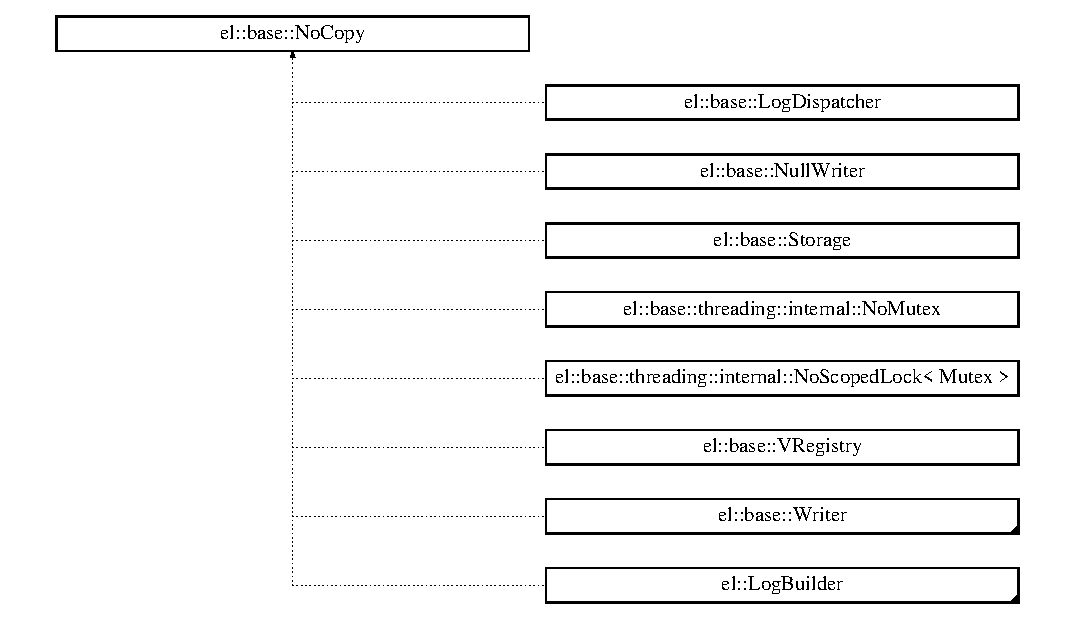
\includegraphics[height=7.875000cm]{classel_1_1base_1_1NoCopy}
\end{center}
\end{figure}


\subsection{Detailed Description}
Internal helper class that prevent copy constructor for class. 

When using this class simply inherit it privately 

The documentation for this class was generated from the following file\-:\begin{DoxyCompactItemize}
\item 
/users/disk9/cfse/\-Stage\-\_\-\-Malo/\-C\-P\-A\-C\-S\-Creator\-Lib/\-C\-P\-A\-C\-S\-Creator\-Lib/easylogging++.\-h\end{DoxyCompactItemize}

\hypertarget{classel_1_1base_1_1threading_1_1internal_1_1NoMutex}{\section{el\-:\-:base\-:\-:threading\-:\-:internal\-:\-:No\-Mutex Class Reference}
\label{classel_1_1base_1_1threading_1_1internal_1_1NoMutex}\index{el\-::base\-::threading\-::internal\-::\-No\-Mutex@{el\-::base\-::threading\-::internal\-::\-No\-Mutex}}
}


Mutex wrapper used when multi-\/threading is disabled.  




{\ttfamily \#include $<$easylogging++.\-h$>$}

Inheritance diagram for el\-:\-:base\-:\-:threading\-:\-:internal\-:\-:No\-Mutex\-:\begin{figure}[H]
\begin{center}
\leavevmode
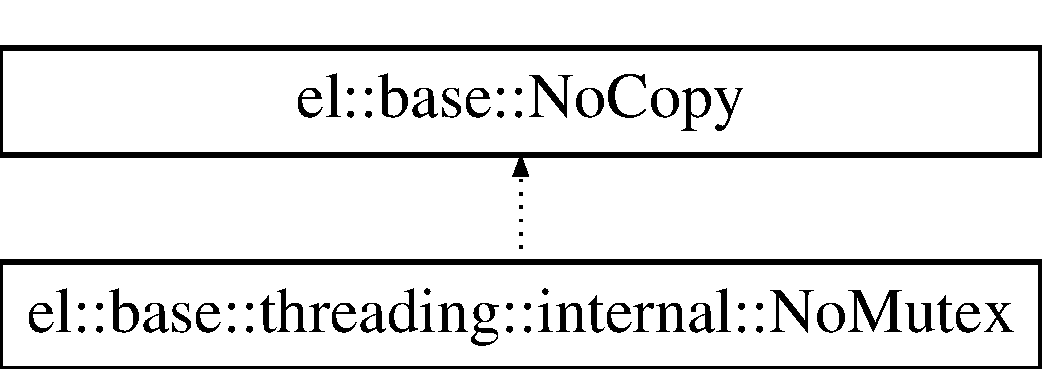
\includegraphics[height=2.000000cm]{classel_1_1base_1_1threading_1_1internal_1_1NoMutex}
\end{center}
\end{figure}
\subsection*{Public Member Functions}
\begin{DoxyCompactItemize}
\item 
\hypertarget{classel_1_1base_1_1threading_1_1internal_1_1NoMutex_a3b38e4e9411c924daa70d358cf561b3c}{void {\bfseries lock} (void)}\label{classel_1_1base_1_1threading_1_1internal_1_1NoMutex_a3b38e4e9411c924daa70d358cf561b3c}

\item 
\hypertarget{classel_1_1base_1_1threading_1_1internal_1_1NoMutex_a4c0c35a99cf41f26a7608fed5609d6ae}{bool {\bfseries try\-\_\-lock} (void)}\label{classel_1_1base_1_1threading_1_1internal_1_1NoMutex_a4c0c35a99cf41f26a7608fed5609d6ae}

\item 
\hypertarget{classel_1_1base_1_1threading_1_1internal_1_1NoMutex_a5a248c97fee2ef0087526f2f8d3cd26e}{void {\bfseries unlock} (void)}\label{classel_1_1base_1_1threading_1_1internal_1_1NoMutex_a5a248c97fee2ef0087526f2f8d3cd26e}

\end{DoxyCompactItemize}


\subsection{Detailed Description}
Mutex wrapper used when multi-\/threading is disabled. 

The documentation for this class was generated from the following file\-:\begin{DoxyCompactItemize}
\item 
/users/disk9/cfse/\-Stage\-\_\-\-Malo/\-C\-P\-A\-C\-S\-Creator\-Lib/\-C\-P\-A\-C\-S\-Creator\-Lib/easylogging++.\-h\end{DoxyCompactItemize}

\hypertarget{classel_1_1base_1_1threading_1_1internal_1_1NoScopedLock}{\section{el\-:\-:base\-:\-:threading\-:\-:internal\-:\-:No\-Scoped\-Lock$<$ Mutex $>$ Class Template Reference}
\label{classel_1_1base_1_1threading_1_1internal_1_1NoScopedLock}\index{el\-::base\-::threading\-::internal\-::\-No\-Scoped\-Lock$<$ Mutex $>$@{el\-::base\-::threading\-::internal\-::\-No\-Scoped\-Lock$<$ Mutex $>$}}
}


Lock guard wrapper used when multi-\/threading is disabled.  




{\ttfamily \#include $<$easylogging++.\-h$>$}

Inheritance diagram for el\-:\-:base\-:\-:threading\-:\-:internal\-:\-:No\-Scoped\-Lock$<$ Mutex $>$\-:\begin{figure}[H]
\begin{center}
\leavevmode
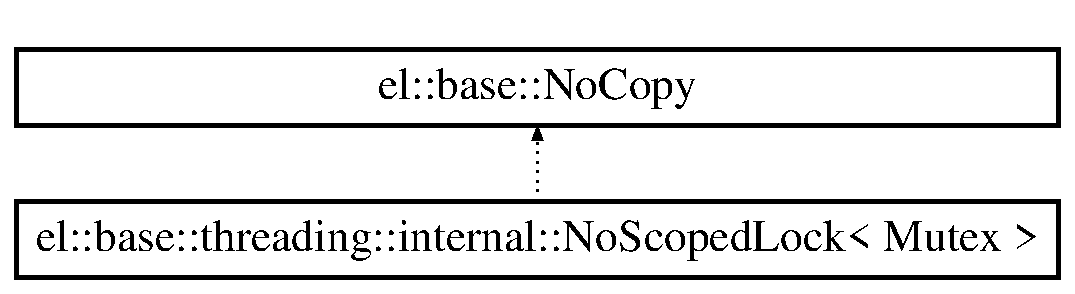
\includegraphics[height=2.000000cm]{classel_1_1base_1_1threading_1_1internal_1_1NoScopedLock}
\end{center}
\end{figure}
\subsection*{Public Member Functions}
\begin{DoxyCompactItemize}
\item 
\hypertarget{classel_1_1base_1_1threading_1_1internal_1_1NoScopedLock_a020f8cea6e83f40ea29662ef57a58235}{{\bfseries No\-Scoped\-Lock} (\hyperlink{classel_1_1base_1_1threading_1_1internal_1_1NoMutex}{Mutex} \&)}\label{classel_1_1base_1_1threading_1_1internal_1_1NoScopedLock_a020f8cea6e83f40ea29662ef57a58235}

\end{DoxyCompactItemize}


\subsection{Detailed Description}
\subsubsection*{template$<$typename Mutex$>$class el\-::base\-::threading\-::internal\-::\-No\-Scoped\-Lock$<$ Mutex $>$}

Lock guard wrapper used when multi-\/threading is disabled. 

The documentation for this class was generated from the following file\-:\begin{DoxyCompactItemize}
\item 
/users/disk9/cfse/\-Stage\-\_\-\-Malo/\-C\-P\-A\-C\-S\-Creator\-Lib/\-C\-P\-A\-C\-S\-Creator\-Lib/easylogging++.\-h\end{DoxyCompactItemize}

\hypertarget{classel_1_1base_1_1NullWriter}{\section{el\-:\-:base\-:\-:Null\-Writer Class Reference}
\label{classel_1_1base_1_1NullWriter}\index{el\-::base\-::\-Null\-Writer@{el\-::base\-::\-Null\-Writer}}
}


Writes nothing -\/ Used when certain log is disabled.  




{\ttfamily \#include $<$easylogging++.\-h$>$}

Inheritance diagram for el\-:\-:base\-:\-:Null\-Writer\-:\begin{figure}[H]
\begin{center}
\leavevmode
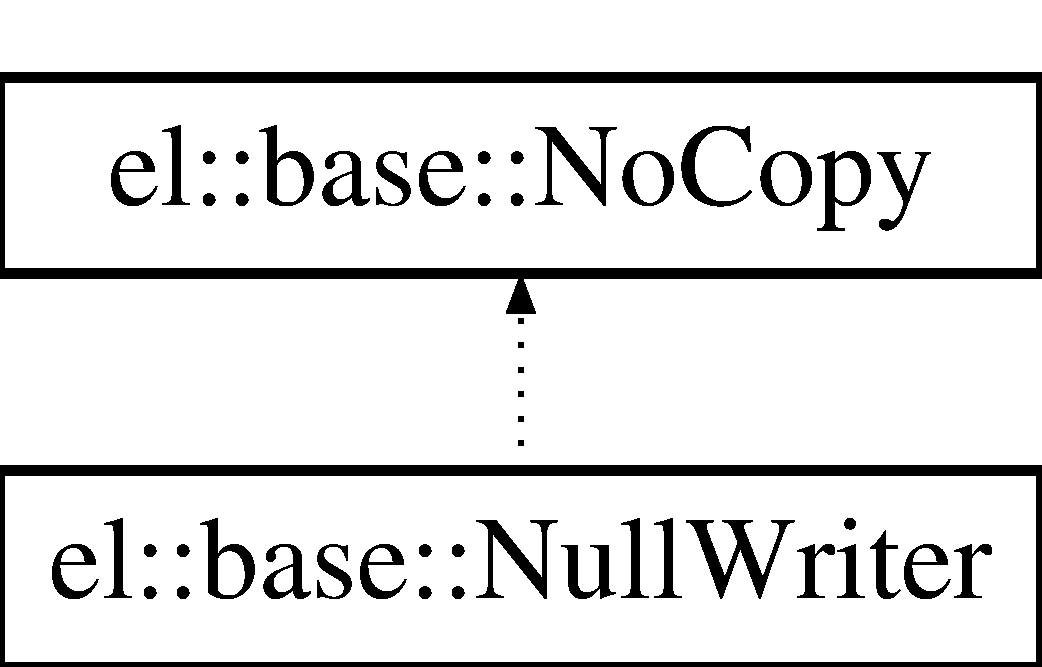
\includegraphics[height=2.000000cm]{classel_1_1base_1_1NullWriter}
\end{center}
\end{figure}
\subsection*{Public Member Functions}
\begin{DoxyCompactItemize}
\item 
\hypertarget{classel_1_1base_1_1NullWriter_a39cb7d47986d70c2b4e9d78d1482da7d}{\hyperlink{classel_1_1base_1_1NullWriter}{Null\-Writer} \& {\bfseries operator$<$$<$} (std\-::ostream \&($\ast$)(std\-::ostream \&))}\label{classel_1_1base_1_1NullWriter_a39cb7d47986d70c2b4e9d78d1482da7d}

\item 
\hypertarget{classel_1_1base_1_1NullWriter_a57cb0f5d93ebac076b8ef94d6eff65a2}{{\footnotesize template$<$typename T $>$ }\\\hyperlink{classel_1_1base_1_1NullWriter}{Null\-Writer} \& {\bfseries operator$<$$<$} (const T \&)}\label{classel_1_1base_1_1NullWriter_a57cb0f5d93ebac076b8ef94d6eff65a2}

\item 
\hypertarget{classel_1_1base_1_1NullWriter_a0d1313fd900f548bb67bc1a1785a4048}{{\bfseries operator bool} ()}\label{classel_1_1base_1_1NullWriter_a0d1313fd900f548bb67bc1a1785a4048}

\end{DoxyCompactItemize}


\subsection{Detailed Description}
Writes nothing -\/ Used when certain log is disabled. 

The documentation for this class was generated from the following file\-:\begin{DoxyCompactItemize}
\item 
/users/disk9/cfse/\-Stage\-\_\-\-Malo/\-C\-P\-A\-C\-S\-Creator\-Lib/\-C\-P\-A\-C\-S\-Creator\-Lib/easylogging++.\-h\end{DoxyCompactItemize}

\hypertarget{classel_1_1base_1_1utils_1_1OS}{\section{el\-:\-:base\-:\-:utils\-:\-:O\-S Class Reference}
\label{classel_1_1base_1_1utils_1_1OS}\index{el\-::base\-::utils\-::\-O\-S@{el\-::base\-::utils\-::\-O\-S}}
}


Operating System helper static class used internally. You should not use it.  




{\ttfamily \#include $<$easylogging++.\-h$>$}

Inheritance diagram for el\-:\-:base\-:\-:utils\-:\-:O\-S\-:\begin{figure}[H]
\begin{center}
\leavevmode
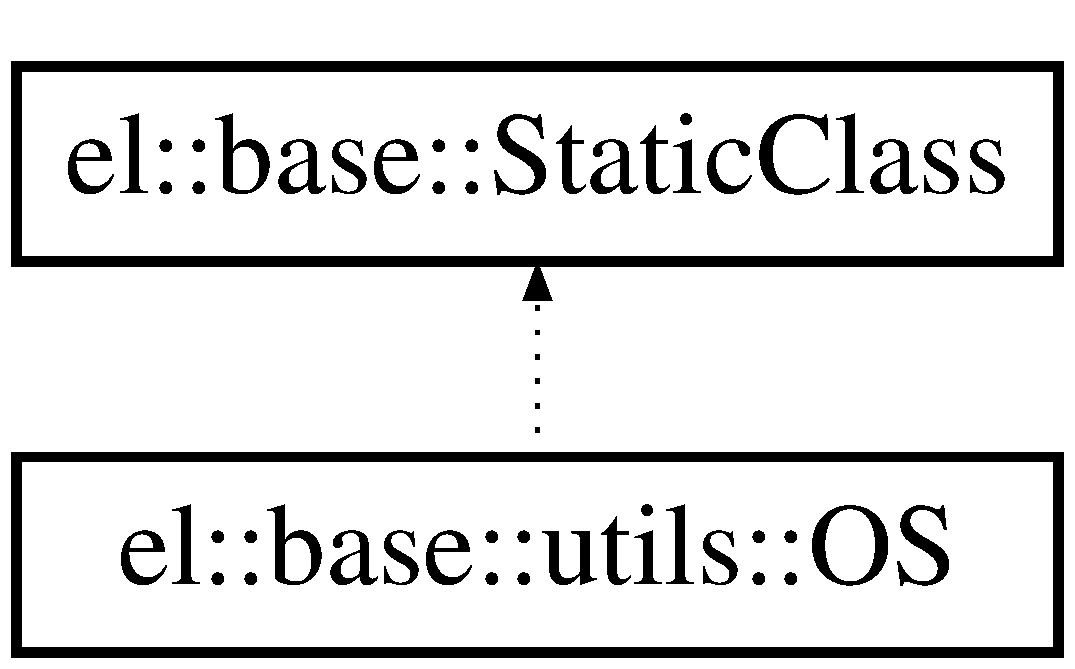
\includegraphics[height=2.000000cm]{classel_1_1base_1_1utils_1_1OS}
\end{center}
\end{figure}
\subsection*{Static Public Member Functions}
\begin{DoxyCompactItemize}
\item 
static const std\-::string \hyperlink{classel_1_1base_1_1utils_1_1OS_a91304c76c872459eaa9fdb3466367cd3}{get\-Bash\-Output} (const char $\ast$command)
\begin{DoxyCompactList}\small\item\em Runs command on terminal and returns the output. \end{DoxyCompactList}\item 
static std\-::string \hyperlink{classel_1_1base_1_1utils_1_1OS_a91540f3d8c87bd121e55fc39270eac3c}{get\-Environment\-Variable} (const char $\ast$variable\-Name, const char $\ast$default\-Val, const char $\ast$alternative\-Bash\-Command=nullptr)
\begin{DoxyCompactList}\small\item\em Gets environment variable. This is cross-\/platform and C\-R\-T safe (for V\-C++) \end{DoxyCompactList}\item 
\hypertarget{classel_1_1base_1_1utils_1_1OS_ac7839ecd50e379dbdfcfce130906386e}{static std\-::string \hyperlink{classel_1_1base_1_1utils_1_1OS_ac7839ecd50e379dbdfcfce130906386e}{current\-User} (void)}\label{classel_1_1base_1_1utils_1_1OS_ac7839ecd50e379dbdfcfce130906386e}

\begin{DoxyCompactList}\small\item\em Gets current username. \end{DoxyCompactList}\item 
static std\-::string \hyperlink{classel_1_1base_1_1utils_1_1OS_aae4fdf83828228fc440f8a875c5942b0}{current\-Host} (void)
\begin{DoxyCompactList}\small\item\em Gets current host name or computer name. \end{DoxyCompactList}\item 
\hypertarget{classel_1_1base_1_1utils_1_1OS_a2c941329a14ce0ea920f57779857864c}{static bool \hyperlink{classel_1_1base_1_1utils_1_1OS_a2c941329a14ce0ea920f57779857864c}{term\-Supports\-Color} (void)}\label{classel_1_1base_1_1utils_1_1OS_a2c941329a14ce0ea920f57779857864c}

\begin{DoxyCompactList}\small\item\em Whether or not terminal supports colors. \end{DoxyCompactList}\end{DoxyCompactItemize}


\subsection{Detailed Description}
Operating System helper static class used internally. You should not use it. 

\subsection{Member Function Documentation}
\hypertarget{classel_1_1base_1_1utils_1_1OS_aae4fdf83828228fc440f8a875c5942b0}{\index{el\-::base\-::utils\-::\-O\-S@{el\-::base\-::utils\-::\-O\-S}!current\-Host@{current\-Host}}
\index{current\-Host@{current\-Host}!el::base::utils::OS@{el\-::base\-::utils\-::\-O\-S}}
\subsubsection[{current\-Host}]{\setlength{\rightskip}{0pt plus 5cm}static std\-::string el\-::base\-::utils\-::\-O\-S\-::current\-Host (
\begin{DoxyParamCaption}
\item[{void}]{}
\end{DoxyParamCaption}
)\hspace{0.3cm}{\ttfamily [static]}}}\label{classel_1_1base_1_1utils_1_1OS_aae4fdf83828228fc440f8a875c5942b0}


Gets current host name or computer name. 

For android systems this is device name with its manufacturer and model seperated by hyphen \hypertarget{classel_1_1base_1_1utils_1_1OS_a91304c76c872459eaa9fdb3466367cd3}{\index{el\-::base\-::utils\-::\-O\-S@{el\-::base\-::utils\-::\-O\-S}!get\-Bash\-Output@{get\-Bash\-Output}}
\index{get\-Bash\-Output@{get\-Bash\-Output}!el::base::utils::OS@{el\-::base\-::utils\-::\-O\-S}}
\subsubsection[{get\-Bash\-Output}]{\setlength{\rightskip}{0pt plus 5cm}static const std\-::string el\-::base\-::utils\-::\-O\-S\-::get\-Bash\-Output (
\begin{DoxyParamCaption}
\item[{const char $\ast$}]{command}
\end{DoxyParamCaption}
)\hspace{0.3cm}{\ttfamily [static]}}}\label{classel_1_1base_1_1utils_1_1OS_a91304c76c872459eaa9fdb3466367cd3}


Runs command on terminal and returns the output. 

This is applicable only on unix based systems, for all other \hyperlink{classel_1_1base_1_1utils_1_1OS}{O\-S}, an empty string is returned. 
\begin{DoxyParams}{Parameters}
{\em command} & Bash command \\
\hline
\end{DoxyParams}
\begin{DoxyReturn}{Returns}
Result of bash output or empty string if no result found. 
\end{DoxyReturn}
\hypertarget{classel_1_1base_1_1utils_1_1OS_a91540f3d8c87bd121e55fc39270eac3c}{\index{el\-::base\-::utils\-::\-O\-S@{el\-::base\-::utils\-::\-O\-S}!get\-Environment\-Variable@{get\-Environment\-Variable}}
\index{get\-Environment\-Variable@{get\-Environment\-Variable}!el::base::utils::OS@{el\-::base\-::utils\-::\-O\-S}}
\subsubsection[{get\-Environment\-Variable}]{\setlength{\rightskip}{0pt plus 5cm}static std\-::string el\-::base\-::utils\-::\-O\-S\-::get\-Environment\-Variable (
\begin{DoxyParamCaption}
\item[{const char $\ast$}]{variable\-Name, }
\item[{const char $\ast$}]{default\-Val, }
\item[{const char $\ast$}]{alternative\-Bash\-Command = {\ttfamily nullptr}}
\end{DoxyParamCaption}
)\hspace{0.3cm}{\ttfamily [static]}}}\label{classel_1_1base_1_1utils_1_1OS_a91540f3d8c87bd121e55fc39270eac3c}


Gets environment variable. This is cross-\/platform and C\-R\-T safe (for V\-C++) 


\begin{DoxyParams}{Parameters}
{\em variable\-Name} & Environment variable name \\
\hline
{\em default\-Val} & If no environment variable or value found the value to return by default \\
\hline
{\em alternative\-Bash\-Command} & If environment variable not found what would be alternative bash command in order to look for value user is looking for. E.\-g, for 'user' alternative command will 'whoami' \\
\hline
\end{DoxyParams}


The documentation for this class was generated from the following file\-:\begin{DoxyCompactItemize}
\item 
/users/disk9/cfse/\-Stage\-\_\-\-Malo/\-C\-P\-A\-C\-S\-Creator\-Lib/\-C\-P\-A\-C\-S\-Creator\-Lib/easylogging++.\-h\end{DoxyCompactItemize}

\hypertarget{classel_1_1Configurations_1_1Parser}{\section{el\-:\-:Configurations\-:\-:Parser Class Reference}
\label{classel_1_1Configurations_1_1Parser}\index{el\-::\-Configurations\-::\-Parser@{el\-::\-Configurations\-::\-Parser}}
}


\hyperlink{classel_1_1Configurations_1_1Parser}{Parser} used internally to parse configurations from file or text.  




{\ttfamily \#include $<$easylogging++.\-h$>$}

Inheritance diagram for el\-:\-:Configurations\-:\-:Parser\-:\begin{figure}[H]
\begin{center}
\leavevmode
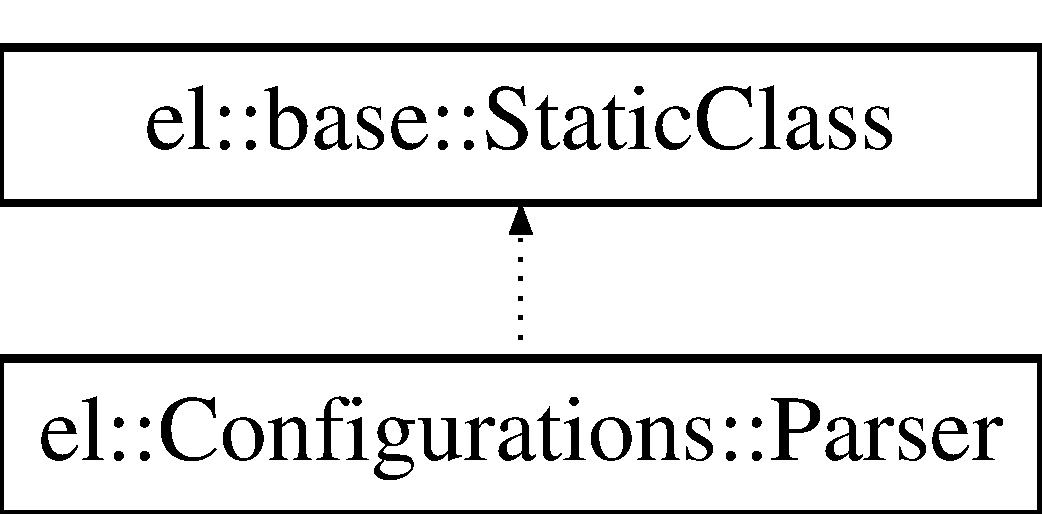
\includegraphics[height=2.000000cm]{classel_1_1Configurations_1_1Parser}
\end{center}
\end{figure}
\subsection*{Static Public Member Functions}
\begin{DoxyCompactItemize}
\item 
static bool \hyperlink{classel_1_1Configurations_1_1Parser_a45def5007bf368c4d2a505af58cd94c2}{parse\-From\-File} (const std\-::string \&\hyperlink{classel_1_1Configurations_a18df64bb5cd97bee672160290133141c}{configuration\-File}, \hyperlink{classel_1_1Configurations}{Configurations} $\ast$sender, \hyperlink{classel_1_1Configurations}{Configurations} $\ast$base=nullptr)
\begin{DoxyCompactList}\small\item\em Parses configuration from file. \end{DoxyCompactList}\item 
static bool \hyperlink{classel_1_1Configurations_1_1Parser_a39ec1b06f673e8155a83d66e08229129}{parse\-From\-Text} (const std\-::string \&configurations\-String, \hyperlink{classel_1_1Configurations}{Configurations} $\ast$sender, \hyperlink{classel_1_1Configurations}{Configurations} $\ast$base=nullptr)
\begin{DoxyCompactList}\small\item\em Parse configurations from configuration string. \end{DoxyCompactList}\end{DoxyCompactItemize}
\subsection*{Friends}
\begin{DoxyCompactItemize}
\item 
\hypertarget{classel_1_1Configurations_1_1Parser_a6efe246b312d02731fb0e1d120c0331d}{class {\bfseries el\-::\-Loggers}}\label{classel_1_1Configurations_1_1Parser_a6efe246b312d02731fb0e1d120c0331d}

\end{DoxyCompactItemize}


\subsection{Detailed Description}
\hyperlink{classel_1_1Configurations_1_1Parser}{Parser} used internally to parse configurations from file or text. 

This class makes use of \hyperlink{classel_1_1base_1_1utils_1_1Str}{base\-::utils\-::\-Str}. You should not need this unless you are working on some tool for Easylogging++ 

\subsection{Member Function Documentation}
\hypertarget{classel_1_1Configurations_1_1Parser_a45def5007bf368c4d2a505af58cd94c2}{\index{el\-::\-Configurations\-::\-Parser@{el\-::\-Configurations\-::\-Parser}!parse\-From\-File@{parse\-From\-File}}
\index{parse\-From\-File@{parse\-From\-File}!el::Configurations::Parser@{el\-::\-Configurations\-::\-Parser}}
\subsubsection[{parse\-From\-File}]{\setlength{\rightskip}{0pt plus 5cm}static bool el\-::\-Configurations\-::\-Parser\-::parse\-From\-File (
\begin{DoxyParamCaption}
\item[{const std\-::string \&}]{configuration\-File, }
\item[{{\bf Configurations} $\ast$}]{sender, }
\item[{{\bf Configurations} $\ast$}]{base = {\ttfamily nullptr}}
\end{DoxyParamCaption}
)\hspace{0.3cm}{\ttfamily [static]}}}\label{classel_1_1Configurations_1_1Parser_a45def5007bf368c4d2a505af58cd94c2}


Parses configuration from file. 


\begin{DoxyParams}{Parameters}
{\em configuration\-File} & Full path to configuration file \\
\hline
{\em sender} & Sender configurations pointer. Usually 'this' is used from calling class \\
\hline
{\em base} & \hyperlink{classel_1_1Configurations}{Configurations} to base new configuration repository off. This value is used when you want to use existing \hyperlink{classel_1_1Configurations}{Configurations} to base all the values and then set rest of configuration via configuration file. \\
\hline
\end{DoxyParams}
\begin{DoxyReturn}{Returns}
True if successfully parsed, false otherwise. You may define '\-\_\-\-S\-T\-O\-P\-\_\-\-O\-N\-\_\-\-F\-I\-R\-S\-T\-E\-L\-P\-P\-\_\-\-A\-S\-S\-E\-R\-T\-I\-O\-N' to make sure you do not proceed without successful parse. 
\end{DoxyReturn}
\hypertarget{classel_1_1Configurations_1_1Parser_a39ec1b06f673e8155a83d66e08229129}{\index{el\-::\-Configurations\-::\-Parser@{el\-::\-Configurations\-::\-Parser}!parse\-From\-Text@{parse\-From\-Text}}
\index{parse\-From\-Text@{parse\-From\-Text}!el::Configurations::Parser@{el\-::\-Configurations\-::\-Parser}}
\subsubsection[{parse\-From\-Text}]{\setlength{\rightskip}{0pt plus 5cm}static bool el\-::\-Configurations\-::\-Parser\-::parse\-From\-Text (
\begin{DoxyParamCaption}
\item[{const std\-::string \&}]{configurations\-String, }
\item[{{\bf Configurations} $\ast$}]{sender, }
\item[{{\bf Configurations} $\ast$}]{base = {\ttfamily nullptr}}
\end{DoxyParamCaption}
)\hspace{0.3cm}{\ttfamily [static]}}}\label{classel_1_1Configurations_1_1Parser_a39ec1b06f673e8155a83d66e08229129}


Parse configurations from configuration string. 

This configuration string has same syntax as configuration file contents. Make sure all the necessary new line characters are provided. You may define '\-\_\-\-S\-T\-O\-P\-\_\-\-O\-N\-\_\-\-F\-I\-R\-S\-T\-E\-L\-P\-P\-\_\-\-A\-S\-S\-E\-R\-T\-I\-O\-N' to make sure you do not proceed without successful parse (This is recommended) 
\begin{DoxyParams}{Parameters}
{\em configurations\-String} & the configuration in plain text format \\
\hline
{\em sender} & Sender configurations pointer. Usually 'this' is used from calling class \\
\hline
{\em base} & \hyperlink{classel_1_1Configurations}{Configurations} to base new configuration repository off. This value is used when you want to use existing \hyperlink{classel_1_1Configurations}{Configurations} to base all the values and then set rest of configuration via configuration text. \\
\hline
\end{DoxyParams}
\begin{DoxyReturn}{Returns}
True if successfully parsed, false otherwise. 
\end{DoxyReturn}


The documentation for this class was generated from the following file\-:\begin{DoxyCompactItemize}
\item 
/users/disk9/cfse/\-Stage\-\_\-\-Malo/\-C\-P\-A\-C\-S\-Creator\-Lib/\-C\-P\-A\-C\-S\-Creator\-Lib/easylogging++.\-h\end{DoxyCompactItemize}

\hypertarget{classel_1_1PerformanceTrackingCallback}{\section{el\-:\-:Performance\-Tracking\-Callback Class Reference}
\label{classel_1_1PerformanceTrackingCallback}\index{el\-::\-Performance\-Tracking\-Callback@{el\-::\-Performance\-Tracking\-Callback}}
}
Inheritance diagram for el\-:\-:Performance\-Tracking\-Callback\-:\begin{figure}[H]
\begin{center}
\leavevmode
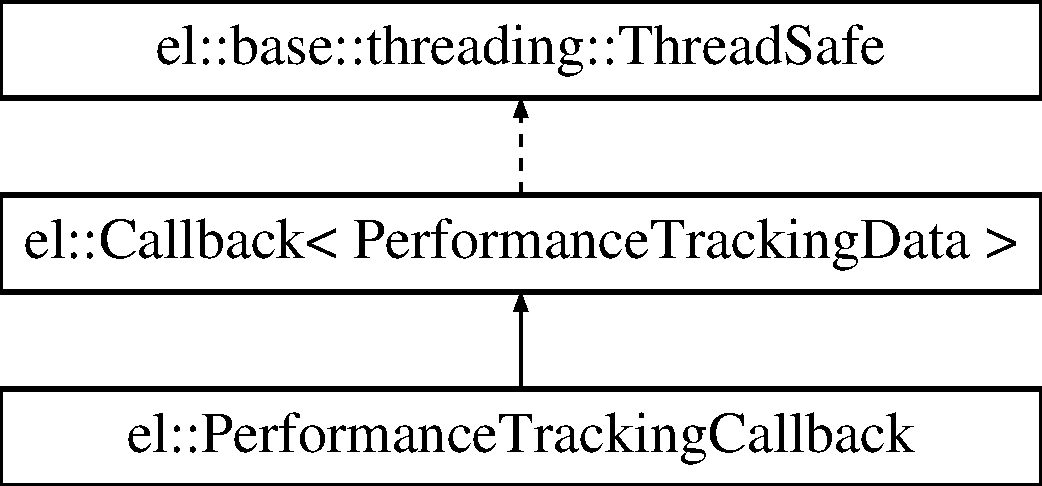
\includegraphics[height=3.000000cm]{classel_1_1PerformanceTrackingCallback}
\end{center}
\end{figure}
\subsection*{Friends}
\begin{DoxyCompactItemize}
\item 
\hypertarget{classel_1_1PerformanceTrackingCallback_a05f271f9cc2531409fe682c6ce0d9feb}{class {\bfseries base\-::\-Performance\-Tracker}}\label{classel_1_1PerformanceTrackingCallback_a05f271f9cc2531409fe682c6ce0d9feb}

\end{DoxyCompactItemize}
\subsection*{Additional Inherited Members}


The documentation for this class was generated from the following file\-:\begin{DoxyCompactItemize}
\item 
/users/disk9/cfse/\-Stage\-\_\-\-Malo/\-C\-P\-A\-C\-S\-Creator\-Lib/\-C\-P\-A\-C\-S\-Creator\-Lib/easylogging++.\-h\end{DoxyCompactItemize}

\hypertarget{classel_1_1base_1_1PErrorWriter}{\section{el\-:\-:base\-:\-:P\-Error\-Writer Class Reference}
\label{classel_1_1base_1_1PErrorWriter}\index{el\-::base\-::\-P\-Error\-Writer@{el\-::base\-::\-P\-Error\-Writer}}
}
Inheritance diagram for el\-:\-:base\-:\-:P\-Error\-Writer\-:\begin{figure}[H]
\begin{center}
\leavevmode
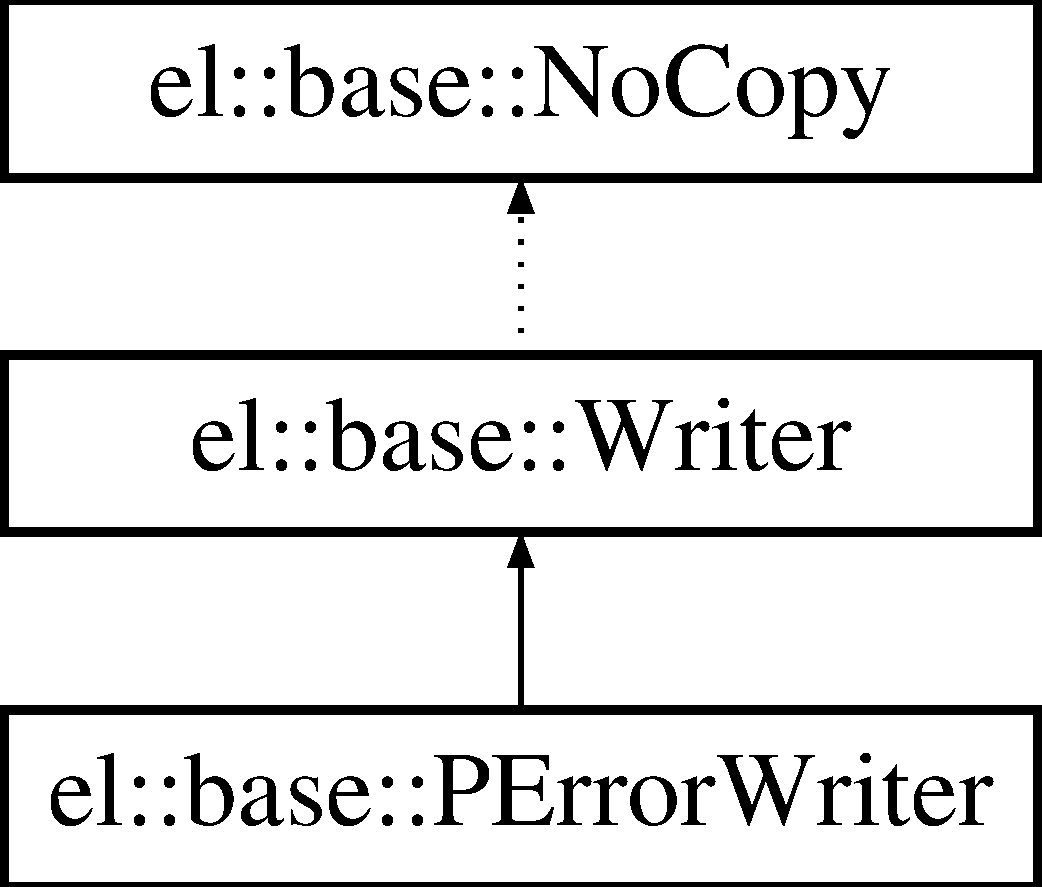
\includegraphics[height=3.000000cm]{classel_1_1base_1_1PErrorWriter}
\end{center}
\end{figure}
\subsection*{Public Member Functions}
\begin{DoxyCompactItemize}
\item 
\hypertarget{classel_1_1base_1_1PErrorWriter_a72c3ef41fd608b5f87ded491957e4c32}{{\bfseries P\-Error\-Writer} (\hyperlink{namespaceel_ab0ac6091262344c52dd2d3ad099e8e36}{Level} level, const char $\ast$file, base\-::type\-::\-Line\-Number line, const char $\ast$func, \hyperlink{namespaceel_1_1base_a3aa2563d38e47388ba242a1694fc2839}{base\-::\-Dispatch\-Action} dispatch\-Action=base\-::\-Dispatch\-Action\-::\-Normal\-Log, base\-::type\-::\-Verbose\-Level verbose\-Level=0)}\label{classel_1_1base_1_1PErrorWriter_a72c3ef41fd608b5f87ded491957e4c32}

\end{DoxyCompactItemize}
\subsection*{Additional Inherited Members}


The documentation for this class was generated from the following file\-:\begin{DoxyCompactItemize}
\item 
/users/disk9/cfse/\-Stage\-\_\-\-Malo/\-C\-P\-A\-C\-S\-Creator\-Lib/\-C\-P\-A\-C\-S\-Creator\-Lib/easylogging++.\-h\end{DoxyCompactItemize}

\hypertarget{classcpcr_1_1Point}{\section{cpcr\-:\-:Point Class Reference}
\label{classcpcr_1_1Point}\index{cpcr\-::\-Point@{cpcr\-::\-Point}}
}
\subsection*{Public Member Functions}
\begin{DoxyCompactItemize}
\item 
\hypertarget{classcpcr_1_1Point_a52b7c586d60a51e86154ba22c58cba6a}{{\bfseries Point} (double xval=0.\-0, double yval=0.\-0, double zval=0.\-0)}\label{classcpcr_1_1Point_a52b7c586d60a51e86154ba22c58cba6a}

\item 
\hypertarget{classcpcr_1_1Point_aa702d5dbc45381601af52d2d1abbe745}{{\bfseries Point} (const std\-::vector$<$ double $>$ \&vector)}\label{classcpcr_1_1Point_aa702d5dbc45381601af52d2d1abbe745}

\item 
\hypertarget{classcpcr_1_1Point_aaccd37e406e6ad9d373bc2e81be61d03}{{\bfseries Point} (const \hyperlink{classcpcr_1_1Point}{Point} \&a\-Point)}\label{classcpcr_1_1Point_aaccd37e406e6ad9d373bc2e81be61d03}

\item 
\hypertarget{classcpcr_1_1Point_a8d5c82dfa5a5f9f2baaf2d2ae19a9f91}{\hyperlink{classcpcr_1_1Point}{Point} \& {\bfseries operator=} (const \hyperlink{classcpcr_1_1Point}{Point} \&a\-Point)}\label{classcpcr_1_1Point_a8d5c82dfa5a5f9f2baaf2d2ae19a9f91}

\item 
\hypertarget{classcpcr_1_1Point_ad1ee707b693656f92055194f2955ba92}{\hyperlink{classcpcr_1_1Point}{Point} {\bfseries operator+} (const \hyperlink{classcpcr_1_1Point}{Point} \&a\-Point) const }\label{classcpcr_1_1Point_ad1ee707b693656f92055194f2955ba92}

\item 
\hypertarget{classcpcr_1_1Point_a2bb6373d0366f396f79392fb9885020f}{\hyperlink{classcpcr_1_1Point}{Point} \& {\bfseries operator+=} (const \hyperlink{classcpcr_1_1Point}{Point} \&a\-Point)}\label{classcpcr_1_1Point_a2bb6373d0366f396f79392fb9885020f}

\item 
\hypertarget{classcpcr_1_1Point_a5d65676b0e1eba9049561b5c4d65f0f2}{\hyperlink{classcpcr_1_1Point}{Point} {\bfseries operator-\/} (const \hyperlink{classcpcr_1_1Point}{Point} \&a\-Point) const }\label{classcpcr_1_1Point_a5d65676b0e1eba9049561b5c4d65f0f2}

\item 
\hypertarget{classcpcr_1_1Point_a809867719e326977963243b3d2e1e6b8}{\hyperlink{classcpcr_1_1Point}{Point} \& {\bfseries operator-\/=} (const \hyperlink{classcpcr_1_1Point}{Point} \&a\-Point)}\label{classcpcr_1_1Point_a809867719e326977963243b3d2e1e6b8}

\item 
\hypertarget{classcpcr_1_1Point_aa964fe220933ab96bec7d2bb07fbee23}{\hyperlink{classcpcr_1_1Point}{Point} {\bfseries operator$\ast$} (double) const }\label{classcpcr_1_1Point_aa964fe220933ab96bec7d2bb07fbee23}

\item 
\hypertarget{classcpcr_1_1Point_a6b055fc8fb84a4b168fe0fda34f2a540}{bool {\bfseries operator==} (const \hyperlink{classcpcr_1_1Point}{Point} \&other)}\label{classcpcr_1_1Point_a6b055fc8fb84a4b168fe0fda34f2a540}

\item 
\hypertarget{classcpcr_1_1Point_a2caa7b00e7faf988ad3bbf98fc38975f}{Eigen\-::\-Vector3d {\bfseries to\-Eigen} () const }\label{classcpcr_1_1Point_a2caa7b00e7faf988ad3bbf98fc38975f}

\item 
\hypertarget{classcpcr_1_1Point_a08544ae3c2ede042658a1b0686751db1}{Eigen\-::\-Vector4d {\bfseries to\-Augmented\-Eigen} () const }\label{classcpcr_1_1Point_a08544ae3c2ede042658a1b0686751db1}

\item 
\hypertarget{classcpcr_1_1Point_a0f2a9aa4650c31abd11fe6d7f838782b}{double {\bfseries norm2\-Sqr} () const }\label{classcpcr_1_1Point_a0f2a9aa4650c31abd11fe6d7f838782b}

\item 
\hypertarget{classcpcr_1_1Point_a224f737024962d348b886535e92c6128}{double {\bfseries norm2} () const }\label{classcpcr_1_1Point_a224f737024962d348b886535e92c6128}

\item 
\hypertarget{classcpcr_1_1Point_a4c465336da011dd6827fa62aeda3e086}{void {\bfseries Dump} (std\-::ostream \&a\-Stream) const }\label{classcpcr_1_1Point_a4c465336da011dd6827fa62aeda3e086}

\item 
\hypertarget{classcpcr_1_1Point_a89999df9f974c8c2b250b3d7547be4ca}{double {\bfseries distance2} (const \hyperlink{classcpcr_1_1Point}{Point} \&point) const }\label{classcpcr_1_1Point_a89999df9f974c8c2b250b3d7547be4ca}

\item 
\hypertarget{classcpcr_1_1Point_aae866ac18021b8bd4f85d114afe87d3c}{void {\bfseries get\-Min\-Max} (double \&min, double \&max) const }\label{classcpcr_1_1Point_aae866ac18021b8bd4f85d114afe87d3c}

\item 
\hypertarget{classcpcr_1_1Point_a43e4302201a34a2b20767470039e7979}{std\-::vector$<$ double $>$ {\bfseries to\-Std\-Vector} ()}\label{classcpcr_1_1Point_a43e4302201a34a2b20767470039e7979}

\end{DoxyCompactItemize}
\subsection*{Static Public Member Functions}
\begin{DoxyCompactItemize}
\item 
\hypertarget{classcpcr_1_1Point_a7d772183814e327af7598e4cc2012721}{static double {\bfseries inner\-\_\-prod} (const \hyperlink{classcpcr_1_1Point}{Point} \&a\-Point, const \hyperlink{classcpcr_1_1Point}{Point} \&b\-Point)}\label{classcpcr_1_1Point_a7d772183814e327af7598e4cc2012721}

\item 
\hypertarget{classcpcr_1_1Point_af592d7e51cce62d1babed5de97b43e69}{static \hyperlink{classcpcr_1_1Point}{Point} {\bfseries cross\-\_\-prod} (const \hyperlink{classcpcr_1_1Point}{Point} \&a, const \hyperlink{classcpcr_1_1Point}{Point} \&b)}\label{classcpcr_1_1Point_af592d7e51cce62d1babed5de97b43e69}

\item 
\hypertarget{classcpcr_1_1Point_a4c5486276fbf5a4d634d5d20b381c04e}{static double {\bfseries scalar\-\_\-projection} (const \hyperlink{classcpcr_1_1Point}{Point} \&a, const \hyperlink{classcpcr_1_1Point}{Point} \&b)}\label{classcpcr_1_1Point_a4c5486276fbf5a4d634d5d20b381c04e}

\item 
\hypertarget{classcpcr_1_1Point_a6c76a72df55e4dc884c746114b9cc43b}{static \hyperlink{classcpcr_1_1Point}{Point} {\bfseries vector\-\_\-projection} (const \hyperlink{classcpcr_1_1Point}{Point} \&a, const \hyperlink{classcpcr_1_1Point}{Point} \&b)}\label{classcpcr_1_1Point_a6c76a72df55e4dc884c746114b9cc43b}

\end{DoxyCompactItemize}
\subsection*{Public Attributes}
\begin{DoxyCompactItemize}
\item 
\hypertarget{classcpcr_1_1Point_a10b516b8c941a39a2e3292cfb7226578}{double {\bfseries x}}\label{classcpcr_1_1Point_a10b516b8c941a39a2e3292cfb7226578}

\item 
\hypertarget{classcpcr_1_1Point_a11fad9d9b998bd29ed7dd43ae70d8446}{double {\bfseries y}}\label{classcpcr_1_1Point_a11fad9d9b998bd29ed7dd43ae70d8446}

\item 
\hypertarget{classcpcr_1_1Point_ac70d54598a9813206e5f7e7ba57756ff}{double {\bfseries z}}\label{classcpcr_1_1Point_ac70d54598a9813206e5f7e7ba57756ff}

\end{DoxyCompactItemize}


The documentation for this class was generated from the following files\-:\begin{DoxyCompactItemize}
\item 
/users/disk9/cfse/\-Stage\-\_\-\-Malo/\-C\-P\-A\-C\-S\-Creator\-Lib/\-C\-P\-A\-C\-S\-Creator\-Lib/\hyperlink{Point_8h}{Point.\-h}\item 
/users/disk9/cfse/\-Stage\-\_\-\-Malo/\-C\-P\-A\-C\-S\-Creator\-Lib/\-C\-P\-A\-C\-S\-Creator\-Lib/\hyperlink{Point_8cpp}{Point.\-cpp}\end{DoxyCompactItemize}

\hypertarget{classel_1_1Configuration_1_1Predicate}{\section{el\-:\-:Configuration\-:\-:Predicate Class Reference}
\label{classel_1_1Configuration_1_1Predicate}\index{el\-::\-Configuration\-::\-Predicate@{el\-::\-Configuration\-::\-Predicate}}
}


Used to find configuration from configuration (pointers) repository. Avoid using it.  




{\ttfamily \#include $<$easylogging++.\-h$>$}

\subsection*{Public Member Functions}
\begin{DoxyCompactItemize}
\item 
\hypertarget{classel_1_1Configuration_1_1Predicate_ab0a4580d6c2d1aaf36a62913fdc38447}{{\bfseries Predicate} (\hyperlink{namespaceel_ab0ac6091262344c52dd2d3ad099e8e36}{Level} \hyperlink{classel_1_1Configuration_a66a96cf46d20204c50718f8a5e3622e2}{level}, \hyperlink{namespaceel_a281f5db6d6163678bc68a8b23b59e124}{Configuration\-Type} \hyperlink{classel_1_1Configuration_aab5091dcca176e309c0a2268ff55db0d}{configuration\-Type})}\label{classel_1_1Configuration_1_1Predicate_ab0a4580d6c2d1aaf36a62913fdc38447}

\item 
\hypertarget{classel_1_1Configuration_1_1Predicate_a985dce44ae06854e789a2ad3be11698f}{bool {\bfseries operator()} (const \hyperlink{classel_1_1Configuration}{Configuration} $\ast$conf) const }\label{classel_1_1Configuration_1_1Predicate_a985dce44ae06854e789a2ad3be11698f}

\end{DoxyCompactItemize}


\subsection{Detailed Description}
Used to find configuration from configuration (pointers) repository. Avoid using it. 

The documentation for this class was generated from the following file\-:\begin{DoxyCompactItemize}
\item 
/users/disk9/cfse/\-Stage\-\_\-\-Malo/\-C\-P\-A\-C\-S\-Creator\-Lib/\-C\-P\-A\-C\-S\-Creator\-Lib/easylogging++.\-h\end{DoxyCompactItemize}

\hypertarget{classel_1_1base_1_1HitCounter_1_1Predicate}{\section{el\-:\-:base\-:\-:Hit\-Counter\-:\-:Predicate Class Reference}
\label{classel_1_1base_1_1HitCounter_1_1Predicate}\index{el\-::base\-::\-Hit\-Counter\-::\-Predicate@{el\-::base\-::\-Hit\-Counter\-::\-Predicate}}
}
\subsection*{Public Member Functions}
\begin{DoxyCompactItemize}
\item 
\hypertarget{classel_1_1base_1_1HitCounter_1_1Predicate_a466afee32aca2403bd2113151f930063}{{\bfseries Predicate} (const char $\ast$filename, base\-::type\-::\-Line\-Number line\-Number)}\label{classel_1_1base_1_1HitCounter_1_1Predicate_a466afee32aca2403bd2113151f930063}

\item 
\hypertarget{classel_1_1base_1_1HitCounter_1_1Predicate_ae07b1562a3c0ed38457401e60b80b0c5}{bool {\bfseries operator()} (const \hyperlink{classel_1_1base_1_1HitCounter}{Hit\-Counter} $\ast$counter)}\label{classel_1_1base_1_1HitCounter_1_1Predicate_ae07b1562a3c0ed38457401e60b80b0c5}

\end{DoxyCompactItemize}


The documentation for this class was generated from the following file\-:\begin{DoxyCompactItemize}
\item 
/users/disk9/cfse/\-Stage\-\_\-\-Malo/\-C\-P\-A\-C\-S\-Creator\-Lib/\-C\-P\-A\-C\-S\-Creator\-Lib/easylogging++.\-h\end{DoxyCompactItemize}

\hypertarget{classel_1_1base_1_1RegisteredHitCounters}{\section{el\-:\-:base\-:\-:Registered\-Hit\-Counters Class Reference}
\label{classel_1_1base_1_1RegisteredHitCounters}\index{el\-::base\-::\-Registered\-Hit\-Counters@{el\-::base\-::\-Registered\-Hit\-Counters}}
}


Repository for hit counters used across the application.  




{\ttfamily \#include $<$easylogging++.\-h$>$}

Inheritance diagram for el\-:\-:base\-:\-:Registered\-Hit\-Counters\-:\begin{figure}[H]
\begin{center}
\leavevmode
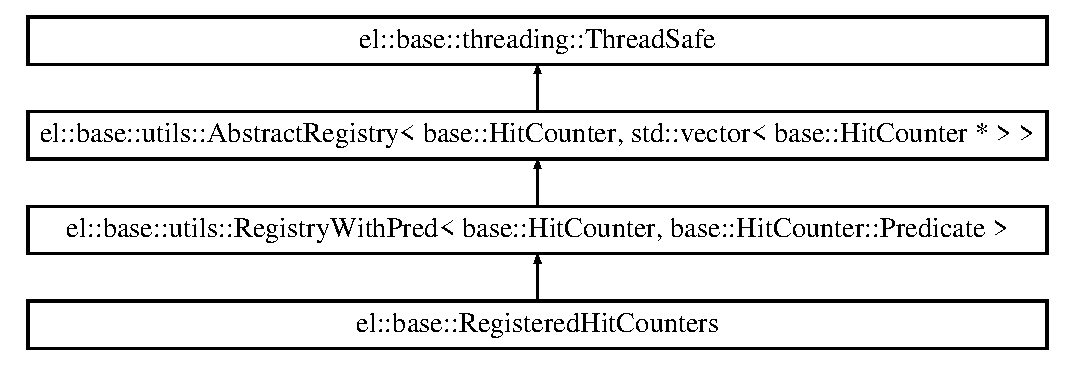
\includegraphics[height=4.000000cm]{classel_1_1base_1_1RegisteredHitCounters}
\end{center}
\end{figure}
\subsection*{Public Member Functions}
\begin{DoxyCompactItemize}
\item 
bool \hyperlink{classel_1_1base_1_1RegisteredHitCounters_a586bb8c5e2722e08a255039bb41e03fa}{validate\-Every\-N} (const char $\ast$filename, base\-::type\-::\-Line\-Number line\-Number, std\-::size\-\_\-t n)
\begin{DoxyCompactList}\small\item\em Validates counter for every N, i.\-e, registers new if does not exist otherwise updates original one. \end{DoxyCompactList}\item 
bool \hyperlink{classel_1_1base_1_1RegisteredHitCounters_ad17bfabd59d2142b57282156483708ef}{validate\-After\-N} (const char $\ast$filename, base\-::type\-::\-Line\-Number line\-Number, std\-::size\-\_\-t n)
\begin{DoxyCompactList}\small\item\em Validates counter for hits $>$= N, i.\-e, registers new if does not exist otherwise updates original one. \end{DoxyCompactList}\item 
bool \hyperlink{classel_1_1base_1_1RegisteredHitCounters_acc7e50a6b720a90714e60d2710fdfbe6}{validate\-N\-Times} (const char $\ast$filename, base\-::type\-::\-Line\-Number line\-Number, std\-::size\-\_\-t n)
\begin{DoxyCompactList}\small\item\em Validates counter for hits are $<$= n, i.\-e, registers new if does not exist otherwise updates original one. \end{DoxyCompactList}\item 
\hypertarget{classel_1_1base_1_1RegisteredHitCounters_ae97474e9e70bcbbde91fb6d6c89cc406}{const \hyperlink{classel_1_1base_1_1HitCounter}{base\-::\-Hit\-Counter} $\ast$ \hyperlink{classel_1_1base_1_1RegisteredHitCounters_ae97474e9e70bcbbde91fb6d6c89cc406}{get\-Counter} (const char $\ast$filename, base\-::type\-::\-Line\-Number line\-Number)}\label{classel_1_1base_1_1RegisteredHitCounters_ae97474e9e70bcbbde91fb6d6c89cc406}

\begin{DoxyCompactList}\small\item\em Gets hit counter registered at specified position. \end{DoxyCompactList}\end{DoxyCompactItemize}
\subsection*{Additional Inherited Members}


\subsection{Detailed Description}
Repository for hit counters used across the application. 

\subsection{Member Function Documentation}
\hypertarget{classel_1_1base_1_1RegisteredHitCounters_ad17bfabd59d2142b57282156483708ef}{\index{el\-::base\-::\-Registered\-Hit\-Counters@{el\-::base\-::\-Registered\-Hit\-Counters}!validate\-After\-N@{validate\-After\-N}}
\index{validate\-After\-N@{validate\-After\-N}!el::base::RegisteredHitCounters@{el\-::base\-::\-Registered\-Hit\-Counters}}
\subsubsection[{validate\-After\-N}]{\setlength{\rightskip}{0pt plus 5cm}bool el\-::base\-::\-Registered\-Hit\-Counters\-::validate\-After\-N (
\begin{DoxyParamCaption}
\item[{const char $\ast$}]{filename, }
\item[{base\-::type\-::\-Line\-Number}]{line\-Number, }
\item[{std\-::size\-\_\-t}]{n}
\end{DoxyParamCaption}
)}}\label{classel_1_1base_1_1RegisteredHitCounters_ad17bfabd59d2142b57282156483708ef}


Validates counter for hits $>$= N, i.\-e, registers new if does not exist otherwise updates original one. 

\begin{DoxyReturn}{Returns}
True if validation resulted in triggering hit. Meaning logs should be written everytime true is returned 
\end{DoxyReturn}
\hypertarget{classel_1_1base_1_1RegisteredHitCounters_a586bb8c5e2722e08a255039bb41e03fa}{\index{el\-::base\-::\-Registered\-Hit\-Counters@{el\-::base\-::\-Registered\-Hit\-Counters}!validate\-Every\-N@{validate\-Every\-N}}
\index{validate\-Every\-N@{validate\-Every\-N}!el::base::RegisteredHitCounters@{el\-::base\-::\-Registered\-Hit\-Counters}}
\subsubsection[{validate\-Every\-N}]{\setlength{\rightskip}{0pt plus 5cm}bool el\-::base\-::\-Registered\-Hit\-Counters\-::validate\-Every\-N (
\begin{DoxyParamCaption}
\item[{const char $\ast$}]{filename, }
\item[{base\-::type\-::\-Line\-Number}]{line\-Number, }
\item[{std\-::size\-\_\-t}]{n}
\end{DoxyParamCaption}
)}}\label{classel_1_1base_1_1RegisteredHitCounters_a586bb8c5e2722e08a255039bb41e03fa}


Validates counter for every N, i.\-e, registers new if does not exist otherwise updates original one. 

\begin{DoxyReturn}{Returns}
True if validation resulted in triggering hit. Meaning logs should be written everytime true is returned 
\end{DoxyReturn}
\hypertarget{classel_1_1base_1_1RegisteredHitCounters_acc7e50a6b720a90714e60d2710fdfbe6}{\index{el\-::base\-::\-Registered\-Hit\-Counters@{el\-::base\-::\-Registered\-Hit\-Counters}!validate\-N\-Times@{validate\-N\-Times}}
\index{validate\-N\-Times@{validate\-N\-Times}!el::base::RegisteredHitCounters@{el\-::base\-::\-Registered\-Hit\-Counters}}
\subsubsection[{validate\-N\-Times}]{\setlength{\rightskip}{0pt plus 5cm}bool el\-::base\-::\-Registered\-Hit\-Counters\-::validate\-N\-Times (
\begin{DoxyParamCaption}
\item[{const char $\ast$}]{filename, }
\item[{base\-::type\-::\-Line\-Number}]{line\-Number, }
\item[{std\-::size\-\_\-t}]{n}
\end{DoxyParamCaption}
)}}\label{classel_1_1base_1_1RegisteredHitCounters_acc7e50a6b720a90714e60d2710fdfbe6}


Validates counter for hits are $<$= n, i.\-e, registers new if does not exist otherwise updates original one. 

\begin{DoxyReturn}{Returns}
True if validation resulted in triggering hit. Meaning logs should be written everytime true is returned 
\end{DoxyReturn}


The documentation for this class was generated from the following file\-:\begin{DoxyCompactItemize}
\item 
/users/disk9/cfse/\-Stage\-\_\-\-Malo/\-C\-P\-A\-C\-S\-Creator\-Lib/\-C\-P\-A\-C\-S\-Creator\-Lib/easylogging++.\-h\end{DoxyCompactItemize}

\hypertarget{classel_1_1base_1_1RegisteredLoggers}{\section{el\-:\-:base\-:\-:Registered\-Loggers Class Reference}
\label{classel_1_1base_1_1RegisteredLoggers}\index{el\-::base\-::\-Registered\-Loggers@{el\-::base\-::\-Registered\-Loggers}}
}


\hyperlink{classel_1_1Loggers}{Loggers} repository.  




{\ttfamily \#include $<$easylogging++.\-h$>$}

Inheritance diagram for el\-:\-:base\-:\-:Registered\-Loggers\-:\begin{figure}[H]
\begin{center}
\leavevmode
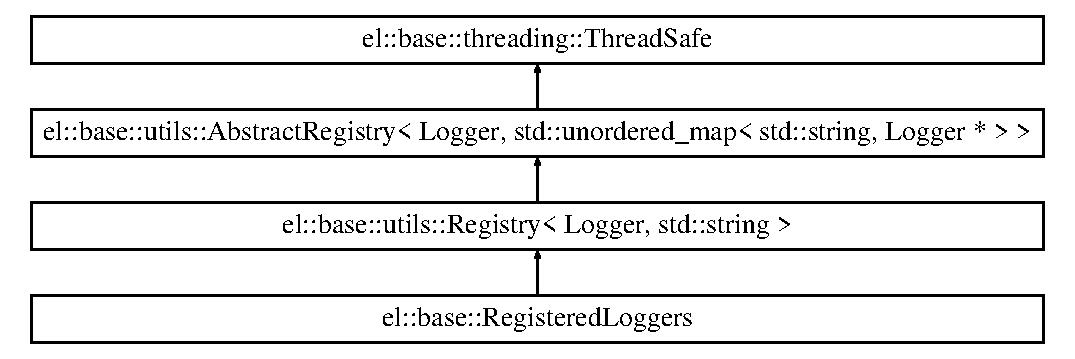
\includegraphics[height=4.000000cm]{classel_1_1base_1_1RegisteredLoggers}
\end{center}
\end{figure}
\subsection*{Public Member Functions}
\begin{DoxyCompactItemize}
\item 
\hypertarget{classel_1_1base_1_1RegisteredLoggers_ae52ec336770d33fef86f234e4e68dce5}{{\bfseries Registered\-Loggers} (const Log\-Builder\-Ptr \&default\-Log\-Builder)}\label{classel_1_1base_1_1RegisteredLoggers_ae52ec336770d33fef86f234e4e68dce5}

\item 
\hypertarget{classel_1_1base_1_1RegisteredLoggers_a28e1f955ad55d89a4ae91fa74545ee4f}{void {\bfseries set\-Default\-Configurations} (const \hyperlink{classel_1_1Configurations}{Configurations} \&configurations)}\label{classel_1_1base_1_1RegisteredLoggers_a28e1f955ad55d89a4ae91fa74545ee4f}

\item 
\hypertarget{classel_1_1base_1_1RegisteredLoggers_acb38f67cf5e297f4be3efa5312e09914}{\hyperlink{classel_1_1Configurations}{Configurations} $\ast$ {\bfseries default\-Configurations} (void)}\label{classel_1_1base_1_1RegisteredLoggers_acb38f67cf5e297f4be3efa5312e09914}

\item 
\hypertarget{classel_1_1base_1_1RegisteredLoggers_a8e554505cd7f66d31e91933b61d74144}{\hyperlink{classel_1_1Logger}{Logger} $\ast$ {\bfseries get} (const std\-::string \&id, bool force\-Creation=true)}\label{classel_1_1base_1_1RegisteredLoggers_a8e554505cd7f66d31e91933b61d74144}

\item 
\hypertarget{classel_1_1base_1_1RegisteredLoggers_a62000b4c52b2383ec7f480ee0fd12586}{{\footnotesize template$<$typename T $>$ }\\bool {\bfseries install\-Logger\-Registration\-Callback} (const std\-::string \&id)}\label{classel_1_1base_1_1RegisteredLoggers_a62000b4c52b2383ec7f480ee0fd12586}

\item 
\hypertarget{classel_1_1base_1_1RegisteredLoggers_ae72594329e082a58ba9e73462d6c5bb5}{{\footnotesize template$<$typename T $>$ }\\void {\bfseries uninstall\-Logger\-Registration\-Callback} (const std\-::string \&id)}\label{classel_1_1base_1_1RegisteredLoggers_ae72594329e082a58ba9e73462d6c5bb5}

\item 
\hypertarget{classel_1_1base_1_1RegisteredLoggers_ae65d8c76311c733f7191867e13ebbe99}{{\footnotesize template$<$typename T $>$ }\\T $\ast$ {\bfseries logger\-Registration\-Callback} (const std\-::string \&id)}\label{classel_1_1base_1_1RegisteredLoggers_ae65d8c76311c733f7191867e13ebbe99}

\item 
\hypertarget{classel_1_1base_1_1RegisteredLoggers_a4d17dc9673f6aa6216571e182097400a}{bool {\bfseries remove} (const std\-::string \&id)}\label{classel_1_1base_1_1RegisteredLoggers_a4d17dc9673f6aa6216571e182097400a}

\item 
\hypertarget{classel_1_1base_1_1RegisteredLoggers_a85916925e2c53d1ebf9865625132a0be}{bool {\bfseries has} (const std\-::string \&id)}\label{classel_1_1base_1_1RegisteredLoggers_a85916925e2c53d1ebf9865625132a0be}

\item 
\hypertarget{classel_1_1base_1_1RegisteredLoggers_ad8fa8f829fdb6a03e6f5a38704811e7b}{void {\bfseries unregister} (\hyperlink{classel_1_1Logger}{Logger} $\ast$\&logger)}\label{classel_1_1base_1_1RegisteredLoggers_ad8fa8f829fdb6a03e6f5a38704811e7b}

\item 
\hypertarget{classel_1_1base_1_1RegisteredLoggers_a11eb24bac74b7ae2d85b324fed707819}{base\-::\-Log\-Streams\-Reference\-Map $\ast$ {\bfseries log\-Streams\-Reference} (void)}\label{classel_1_1base_1_1RegisteredLoggers_a11eb24bac74b7ae2d85b324fed707819}

\item 
\hypertarget{classel_1_1base_1_1RegisteredLoggers_abe6fdac67d9d4c35fb48c9fd88a49c2e}{void {\bfseries flush\-All} (void)}\label{classel_1_1base_1_1RegisteredLoggers_abe6fdac67d9d4c35fb48c9fd88a49c2e}

\item 
\hypertarget{classel_1_1base_1_1RegisteredLoggers_afccc4cf83c77e97cf7377513094b61a6}{void {\bfseries set\-Default\-Log\-Builder} (Log\-Builder\-Ptr \&log\-Builder\-Ptr)}\label{classel_1_1base_1_1RegisteredLoggers_afccc4cf83c77e97cf7377513094b61a6}

\end{DoxyCompactItemize}
\subsection*{Friends}
\begin{DoxyCompactItemize}
\item 
\hypertarget{classel_1_1base_1_1RegisteredLoggers_acc1efd1b8a3fc5e0028dab98b02e550a}{class {\bfseries el\-::base\-::\-Storage}}\label{classel_1_1base_1_1RegisteredLoggers_acc1efd1b8a3fc5e0028dab98b02e550a}

\end{DoxyCompactItemize}
\subsection*{Additional Inherited Members}


\subsection{Detailed Description}
\hyperlink{classel_1_1Loggers}{Loggers} repository. 

The documentation for this class was generated from the following file\-:\begin{DoxyCompactItemize}
\item 
/users/disk9/cfse/\-Stage\-\_\-\-Malo/\-C\-P\-A\-C\-S\-Creator\-Lib/\-C\-P\-A\-C\-S\-Creator\-Lib/easylogging++.\-h\end{DoxyCompactItemize}

\hypertarget{classel_1_1base_1_1utils_1_1Registry}{\section{el\-:\-:base\-:\-:utils\-:\-:Registry$<$ T\-\_\-\-Ptr, T\-\_\-\-Key $>$ Class Template Reference}
\label{classel_1_1base_1_1utils_1_1Registry}\index{el\-::base\-::utils\-::\-Registry$<$ T\-\_\-\-Ptr, T\-\_\-\-Key $>$@{el\-::base\-::utils\-::\-Registry$<$ T\-\_\-\-Ptr, T\-\_\-\-Key $>$}}
}


A pointer registry mechanism to manage memory and provide search functionalities. (non-\/predicate version)  




{\ttfamily \#include $<$easylogging++.\-h$>$}

Inheritance diagram for el\-:\-:base\-:\-:utils\-:\-:Registry$<$ T\-\_\-\-Ptr, T\-\_\-\-Key $>$\-:\begin{figure}[H]
\begin{center}
\leavevmode
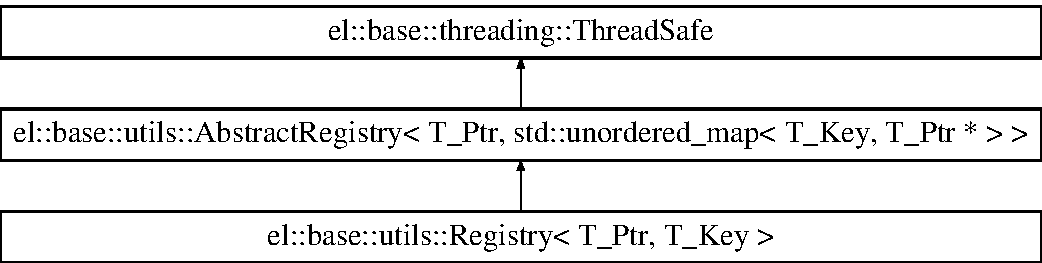
\includegraphics[height=3.000000cm]{classel_1_1base_1_1utils_1_1Registry}
\end{center}
\end{figure}
\subsection*{Public Types}
\begin{DoxyCompactItemize}
\item 
\hypertarget{classel_1_1base_1_1utils_1_1Registry_a31f3d725285e6b65f1f9e990066f96ed}{typedef \hyperlink{classel_1_1base_1_1utils_1_1Registry}{Registry}$<$ T\-\_\-\-Ptr, T\-\_\-\-Key $>$\\*
\-::iterator {\bfseries iterator}}\label{classel_1_1base_1_1utils_1_1Registry_a31f3d725285e6b65f1f9e990066f96ed}

\item 
\hypertarget{classel_1_1base_1_1utils_1_1Registry_a955e62adc74c60d0205b52a3fc430cef}{typedef \hyperlink{classel_1_1base_1_1utils_1_1Registry}{Registry}$<$ T\-\_\-\-Ptr, T\-\_\-\-Key $>$\\*
\-::const\-\_\-iterator {\bfseries const\-\_\-iterator}}\label{classel_1_1base_1_1utils_1_1Registry_a955e62adc74c60d0205b52a3fc430cef}

\end{DoxyCompactItemize}
\subsection*{Public Member Functions}
\begin{DoxyCompactItemize}
\item 
\hypertarget{classel_1_1base_1_1utils_1_1Registry_adf5e97aa801be3b93e116ad645304759}{\hyperlink{classel_1_1base_1_1utils_1_1Registry_adf5e97aa801be3b93e116ad645304759}{Registry} (const \hyperlink{classel_1_1base_1_1utils_1_1Registry}{Registry} \&sr)}\label{classel_1_1base_1_1utils_1_1Registry_adf5e97aa801be3b93e116ad645304759}

\begin{DoxyCompactList}\small\item\em Copy constructor that is useful for base classes. Try to avoid this constructor, use move constructor. \end{DoxyCompactList}\item 
\hyperlink{classel_1_1base_1_1utils_1_1Registry}{Registry} \& \hyperlink{classel_1_1base_1_1utils_1_1Registry_a80e0ce12b7d0c24462b385fc7b3149e0}{operator=} (const \hyperlink{classel_1_1base_1_1utils_1_1Registry}{Registry} \&sr)
\begin{DoxyCompactList}\small\item\em Assignment operator that unregisters all the existing registeries and deeply copies each of repo element. \end{DoxyCompactList}\end{DoxyCompactItemize}
\subsection*{Protected Member Functions}
\begin{DoxyCompactItemize}
\item 
\hypertarget{classel_1_1base_1_1utils_1_1Registry_ac40e62ddf5017beb91c28b472c9628c2}{virtual void \hyperlink{classel_1_1base_1_1utils_1_1Registry_ac40e62ddf5017beb91c28b472c9628c2}{unregister\-All} (void) E\-L\-P\-P\-\_\-\-F\-I\-N\-A\-L}\label{classel_1_1base_1_1utils_1_1Registry_ac40e62ddf5017beb91c28b472c9628c2}

\begin{DoxyCompactList}\small\item\em Unregisters all the pointers from current repository. \end{DoxyCompactList}\item 
\hypertarget{classel_1_1base_1_1utils_1_1Registry_ab10b3dd25ff0df036e7a015635a15dee}{virtual void \hyperlink{classel_1_1base_1_1utils_1_1Registry_ab10b3dd25ff0df036e7a015635a15dee}{register\-New} (const T\-\_\-\-Key \&uniq\-Key, T\-\_\-\-Ptr $\ast$ptr) E\-L\-P\-P\-\_\-\-F\-I\-N\-A\-L}\label{classel_1_1base_1_1utils_1_1Registry_ab10b3dd25ff0df036e7a015635a15dee}

\begin{DoxyCompactList}\small\item\em Registers new registry to repository. \end{DoxyCompactList}\item 
\hypertarget{classel_1_1base_1_1utils_1_1Registry_aab6f0ce3a99feff11add0bd8b869fcb8}{void \hyperlink{classel_1_1base_1_1utils_1_1Registry_aab6f0ce3a99feff11add0bd8b869fcb8}{unregister} (const T\-\_\-\-Key \&uniq\-Key)}\label{classel_1_1base_1_1utils_1_1Registry_aab6f0ce3a99feff11add0bd8b869fcb8}

\begin{DoxyCompactList}\small\item\em Unregisters single entry mapped to specified unique key. \end{DoxyCompactList}\item 
\hypertarget{classel_1_1base_1_1utils_1_1Registry_a18c332267f2acbe78c97a611dec2e5c2}{T\-\_\-\-Ptr $\ast$ \hyperlink{classel_1_1base_1_1utils_1_1Registry_a18c332267f2acbe78c97a611dec2e5c2}{get} (const T\-\_\-\-Key \&uniq\-Key)}\label{classel_1_1base_1_1utils_1_1Registry_a18c332267f2acbe78c97a611dec2e5c2}

\begin{DoxyCompactList}\small\item\em Gets pointer from repository. If none found, nullptr is returned. \end{DoxyCompactList}\end{DoxyCompactItemize}


\subsection{Detailed Description}
\subsubsection*{template$<$typename T\-\_\-\-Ptr, typename T\-\_\-\-Key = const char$\ast$$>$class el\-::base\-::utils\-::\-Registry$<$ T\-\_\-\-Ptr, T\-\_\-\-Key $>$}

A pointer registry mechanism to manage memory and provide search functionalities. (non-\/predicate version) 

N\-O\-T\-E\-: This is thread-\/unsafe implementation (although it contains lock function, it does not use these functions) of Abstract\-Registry$<$\-T\-\_\-\-Ptr, Container$>$. Any implementation of this class should be explicitly (by using lock functions) 

\subsection{Member Function Documentation}
\hypertarget{classel_1_1base_1_1utils_1_1Registry_a80e0ce12b7d0c24462b385fc7b3149e0}{\index{el\-::base\-::utils\-::\-Registry@{el\-::base\-::utils\-::\-Registry}!operator=@{operator=}}
\index{operator=@{operator=}!el::base::utils::Registry@{el\-::base\-::utils\-::\-Registry}}
\subsubsection[{operator=}]{\setlength{\rightskip}{0pt plus 5cm}template$<$typename T\-\_\-\-Ptr, typename T\-\_\-\-Key = const char$\ast$$>$ {\bf Registry}\& {\bf el\-::base\-::utils\-::\-Registry}$<$ T\-\_\-\-Ptr, T\-\_\-\-Key $>$\-::operator= (
\begin{DoxyParamCaption}
\item[{const {\bf Registry}$<$ T\-\_\-\-Ptr, T\-\_\-\-Key $>$ \&}]{sr}
\end{DoxyParamCaption}
)\hspace{0.3cm}{\ttfamily [inline]}}}\label{classel_1_1base_1_1utils_1_1Registry_a80e0ce12b7d0c24462b385fc7b3149e0}


Assignment operator that unregisters all the existing registeries and deeply copies each of repo element. 

\begin{DoxySeeAlso}{See Also}
\hyperlink{classel_1_1base_1_1utils_1_1Registry_ac40e62ddf5017beb91c28b472c9628c2}{unregister\-All()} 

deep\-Copy(const Abstract\-Registry\&) 
\end{DoxySeeAlso}


The documentation for this class was generated from the following file\-:\begin{DoxyCompactItemize}
\item 
/users/disk9/cfse/\-Stage\-\_\-\-Malo/\-C\-P\-A\-C\-S\-Creator\-Lib/\-C\-P\-A\-C\-S\-Creator\-Lib/easylogging++.\-h\end{DoxyCompactItemize}

\hypertarget{classel_1_1base_1_1utils_1_1RegistryWithPred}{\section{el\-:\-:base\-:\-:utils\-:\-:Registry\-With\-Pred$<$ T\-\_\-\-Ptr, Pred $>$ Class Template Reference}
\label{classel_1_1base_1_1utils_1_1RegistryWithPred}\index{el\-::base\-::utils\-::\-Registry\-With\-Pred$<$ T\-\_\-\-Ptr, Pred $>$@{el\-::base\-::utils\-::\-Registry\-With\-Pred$<$ T\-\_\-\-Ptr, Pred $>$}}
}


A pointer registry mechanism to manage memory and provide search functionalities. (predicate version)  




{\ttfamily \#include $<$easylogging++.\-h$>$}

Inheritance diagram for el\-:\-:base\-:\-:utils\-:\-:Registry\-With\-Pred$<$ T\-\_\-\-Ptr, Pred $>$\-:\begin{figure}[H]
\begin{center}
\leavevmode
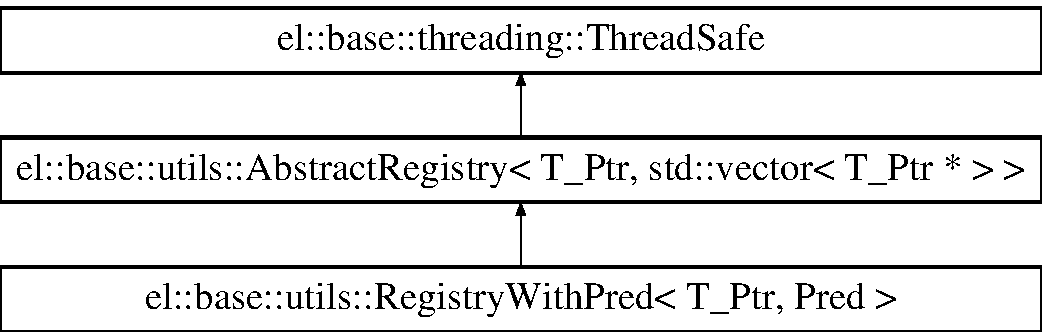
\includegraphics[height=3.000000cm]{classel_1_1base_1_1utils_1_1RegistryWithPred}
\end{center}
\end{figure}
\subsection*{Public Types}
\begin{DoxyCompactItemize}
\item 
\hypertarget{classel_1_1base_1_1utils_1_1RegistryWithPred_afc03d2d0a72f5ebf03e1e3b37bd9932d}{typedef \hyperlink{classel_1_1base_1_1utils_1_1RegistryWithPred}{Registry\-With\-Pred}\\*
$<$ T\-\_\-\-Ptr, Pred $>$\-::iterator {\bfseries iterator}}\label{classel_1_1base_1_1utils_1_1RegistryWithPred_afc03d2d0a72f5ebf03e1e3b37bd9932d}

\item 
\hypertarget{classel_1_1base_1_1utils_1_1RegistryWithPred_ad9af7a8eeedd58a75eb70bccb334f6dc}{typedef \hyperlink{classel_1_1base_1_1utils_1_1RegistryWithPred}{Registry\-With\-Pred}\\*
$<$ T\-\_\-\-Ptr, Pred $>$\\*
\-::const\-\_\-iterator {\bfseries const\-\_\-iterator}}\label{classel_1_1base_1_1utils_1_1RegistryWithPred_ad9af7a8eeedd58a75eb70bccb334f6dc}

\end{DoxyCompactItemize}
\subsection*{Public Member Functions}
\begin{DoxyCompactItemize}
\item 
\hypertarget{classel_1_1base_1_1utils_1_1RegistryWithPred_a0e75c7daaa5fbf824b29180c7a5fd155}{\hyperlink{classel_1_1base_1_1utils_1_1RegistryWithPred_a0e75c7daaa5fbf824b29180c7a5fd155}{Registry\-With\-Pred} (const \hyperlink{classel_1_1base_1_1utils_1_1RegistryWithPred}{Registry\-With\-Pred} \&sr)}\label{classel_1_1base_1_1utils_1_1RegistryWithPred_a0e75c7daaa5fbf824b29180c7a5fd155}

\begin{DoxyCompactList}\small\item\em Copy constructor that is useful for base classes. Try to avoid this constructor, use move constructor. \end{DoxyCompactList}\item 
\hyperlink{classel_1_1base_1_1utils_1_1RegistryWithPred}{Registry\-With\-Pred} \& \hyperlink{classel_1_1base_1_1utils_1_1RegistryWithPred_adb7e568c8cb084589467b937eab86b86}{operator=} (const \hyperlink{classel_1_1base_1_1utils_1_1RegistryWithPred}{Registry\-With\-Pred} \&sr)
\begin{DoxyCompactList}\small\item\em Assignment operator that unregisters all the existing registeries and deeply copies each of repo element. \end{DoxyCompactList}\end{DoxyCompactItemize}
\subsection*{Protected Member Functions}
\begin{DoxyCompactItemize}
\item 
\hypertarget{classel_1_1base_1_1utils_1_1RegistryWithPred_a66b4eca5bb71f3fa3f0737105a00890c}{virtual void \hyperlink{classel_1_1base_1_1utils_1_1RegistryWithPred_a66b4eca5bb71f3fa3f0737105a00890c}{unregister\-All} (void) E\-L\-P\-P\-\_\-\-F\-I\-N\-A\-L}\label{classel_1_1base_1_1utils_1_1RegistryWithPred_a66b4eca5bb71f3fa3f0737105a00890c}

\begin{DoxyCompactList}\small\item\em Unregisters all the pointers from current repository. \end{DoxyCompactList}\item 
\hypertarget{classel_1_1base_1_1utils_1_1RegistryWithPred_aaf1afb5a9f8bd1d99c46ac529ea16417}{virtual void {\bfseries unregister} (T\-\_\-\-Ptr $\ast$\&ptr) E\-L\-P\-P\-\_\-\-F\-I\-N\-A\-L}\label{classel_1_1base_1_1utils_1_1RegistryWithPred_aaf1afb5a9f8bd1d99c46ac529ea16417}

\item 
\hypertarget{classel_1_1base_1_1utils_1_1RegistryWithPred_a561a5d418106a16473ff94d43a4b6b04}{virtual void {\bfseries register\-New} (T\-\_\-\-Ptr $\ast$ptr) E\-L\-P\-P\-\_\-\-F\-I\-N\-A\-L}\label{classel_1_1base_1_1utils_1_1RegistryWithPred_a561a5d418106a16473ff94d43a4b6b04}

\item 
\hypertarget{classel_1_1base_1_1utils_1_1RegistryWithPred_a811d9cc011d945bc7237e6ae1cf2f096}{{\footnotesize template$<$typename T , typename T2 $>$ }\\T\-\_\-\-Ptr $\ast$ \hyperlink{classel_1_1base_1_1utils_1_1RegistryWithPred_a811d9cc011d945bc7237e6ae1cf2f096}{get} (const T \&arg1, const T2 arg2)}\label{classel_1_1base_1_1utils_1_1RegistryWithPred_a811d9cc011d945bc7237e6ae1cf2f096}

\begin{DoxyCompactList}\small\item\em Gets pointer from repository with speicifed arguments. Arguments are passed to predicate in order to validate pointer. \end{DoxyCompactList}\end{DoxyCompactItemize}
\subsection*{Friends}
\begin{DoxyCompactItemize}
\item 
\hypertarget{classel_1_1base_1_1utils_1_1RegistryWithPred_a71b45d148b62604847fe06f7addda779}{base\-::type\-::ostream\-\_\-t \& {\bfseries operator$<$$<$} (base\-::type\-::ostream\-\_\-t \&os, const \hyperlink{classel_1_1base_1_1utils_1_1RegistryWithPred}{Registry\-With\-Pred} \&sr)}\label{classel_1_1base_1_1utils_1_1RegistryWithPred_a71b45d148b62604847fe06f7addda779}

\end{DoxyCompactItemize}


\subsection{Detailed Description}
\subsubsection*{template$<$typename T\-\_\-\-Ptr, typename Pred$>$class el\-::base\-::utils\-::\-Registry\-With\-Pred$<$ T\-\_\-\-Ptr, Pred $>$}

A pointer registry mechanism to manage memory and provide search functionalities. (predicate version) 

N\-O\-T\-E\-: This is thread-\/unsafe implementation of Abstract\-Registry$<$\-T\-\_\-\-Ptr, Container$>$. Any implementation of this class should be made thread-\/safe explicitly 

\subsection{Member Function Documentation}
\hypertarget{classel_1_1base_1_1utils_1_1RegistryWithPred_adb7e568c8cb084589467b937eab86b86}{\index{el\-::base\-::utils\-::\-Registry\-With\-Pred@{el\-::base\-::utils\-::\-Registry\-With\-Pred}!operator=@{operator=}}
\index{operator=@{operator=}!el::base::utils::RegistryWithPred@{el\-::base\-::utils\-::\-Registry\-With\-Pred}}
\subsubsection[{operator=}]{\setlength{\rightskip}{0pt plus 5cm}template$<$typename T\-\_\-\-Ptr, typename Pred$>$ {\bf Registry\-With\-Pred}\& {\bf el\-::base\-::utils\-::\-Registry\-With\-Pred}$<$ T\-\_\-\-Ptr, Pred $>$\-::operator= (
\begin{DoxyParamCaption}
\item[{const {\bf Registry\-With\-Pred}$<$ T\-\_\-\-Ptr, Pred $>$ \&}]{sr}
\end{DoxyParamCaption}
)\hspace{0.3cm}{\ttfamily [inline]}}}\label{classel_1_1base_1_1utils_1_1RegistryWithPred_adb7e568c8cb084589467b937eab86b86}


Assignment operator that unregisters all the existing registeries and deeply copies each of repo element. 

\begin{DoxySeeAlso}{See Also}
\hyperlink{classel_1_1base_1_1utils_1_1RegistryWithPred_a66b4eca5bb71f3fa3f0737105a00890c}{unregister\-All()} 

deep\-Copy(const Abstract\-Registry\&) 
\end{DoxySeeAlso}


The documentation for this class was generated from the following file\-:\begin{DoxyCompactItemize}
\item 
/users/disk9/cfse/\-Stage\-\_\-\-Malo/\-C\-P\-A\-C\-S\-Creator\-Lib/\-C\-P\-A\-C\-S\-Creator\-Lib/easylogging++.\-h\end{DoxyCompactItemize}

\hypertarget{classel_1_1Loggers_1_1ScopedAddFlag}{\section{el\-:\-:Loggers\-:\-:Scoped\-Add\-Flag Class Reference}
\label{classel_1_1Loggers_1_1ScopedAddFlag}\index{el\-::\-Loggers\-::\-Scoped\-Add\-Flag@{el\-::\-Loggers\-::\-Scoped\-Add\-Flag}}
}


Adds flag and removes it when scope goes out.  




{\ttfamily \#include $<$easylogging++.\-h$>$}

\subsection*{Public Member Functions}
\begin{DoxyCompactItemize}
\item 
\hypertarget{classel_1_1Loggers_1_1ScopedAddFlag_a13e0b1052cd1a7a15fae63fd6454d598}{{\bfseries Scoped\-Add\-Flag} (\hyperlink{namespaceel_a2784aacd04cb7816ac1c0b20fcbf83cb}{Logging\-Flag} flag)}\label{classel_1_1Loggers_1_1ScopedAddFlag_a13e0b1052cd1a7a15fae63fd6454d598}

\end{DoxyCompactItemize}


\subsection{Detailed Description}
Adds flag and removes it when scope goes out. 

The documentation for this class was generated from the following file\-:\begin{DoxyCompactItemize}
\item 
/users/disk9/cfse/\-Stage\-\_\-\-Malo/\-C\-P\-A\-C\-S\-Creator\-Lib/\-C\-P\-A\-C\-S\-Creator\-Lib/easylogging++.\-h\end{DoxyCompactItemize}

\hypertarget{classel_1_1Loggers_1_1ScopedRemoveFlag}{\section{el\-:\-:Loggers\-:\-:Scoped\-Remove\-Flag Class Reference}
\label{classel_1_1Loggers_1_1ScopedRemoveFlag}\index{el\-::\-Loggers\-::\-Scoped\-Remove\-Flag@{el\-::\-Loggers\-::\-Scoped\-Remove\-Flag}}
}


Removes flag and add it when scope goes out.  




{\ttfamily \#include $<$easylogging++.\-h$>$}

\subsection*{Public Member Functions}
\begin{DoxyCompactItemize}
\item 
\hypertarget{classel_1_1Loggers_1_1ScopedRemoveFlag_a7ae9a1cde34e1145d8b90b639cc12dc1}{{\bfseries Scoped\-Remove\-Flag} (\hyperlink{namespaceel_a2784aacd04cb7816ac1c0b20fcbf83cb}{Logging\-Flag} flag)}\label{classel_1_1Loggers_1_1ScopedRemoveFlag_a7ae9a1cde34e1145d8b90b639cc12dc1}

\end{DoxyCompactItemize}


\subsection{Detailed Description}
Removes flag and add it when scope goes out. 

The documentation for this class was generated from the following file\-:\begin{DoxyCompactItemize}
\item 
/users/disk9/cfse/\-Stage\-\_\-\-Malo/\-C\-P\-A\-C\-S\-Creator\-Lib/\-C\-P\-A\-C\-S\-Creator\-Lib/easylogging++.\-h\end{DoxyCompactItemize}

\hypertarget{classel_1_1base_1_1StaticClass}{\section{el\-:\-:base\-:\-:Static\-Class Class Reference}
\label{classel_1_1base_1_1StaticClass}\index{el\-::base\-::\-Static\-Class@{el\-::base\-::\-Static\-Class}}
}


Internal helper class that makes all default constructors private.  




{\ttfamily \#include $<$easylogging++.\-h$>$}

Inheritance diagram for el\-:\-:base\-:\-:Static\-Class\-:\begin{figure}[H]
\begin{center}
\leavevmode
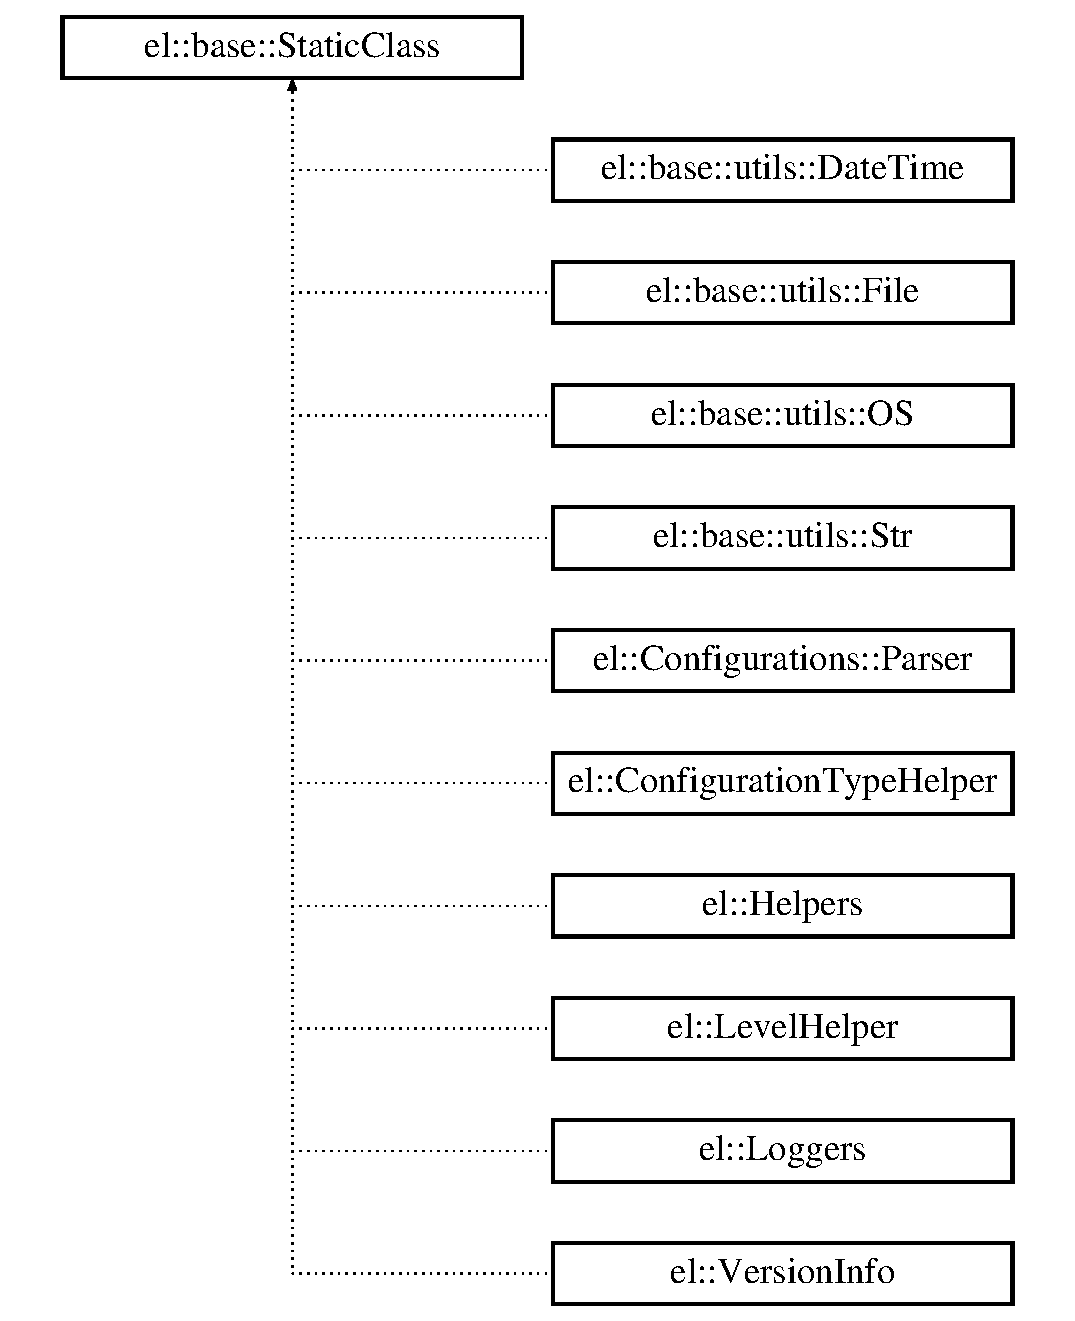
\includegraphics[height=11.000000cm]{classel_1_1base_1_1StaticClass}
\end{center}
\end{figure}


\subsection{Detailed Description}
Internal helper class that makes all default constructors private. 

This prevents initializing class making it static unless an explicit constructor is declared. When using this class simply inherit it privately 

The documentation for this class was generated from the following file\-:\begin{DoxyCompactItemize}
\item 
/users/disk9/cfse/\-Stage\-\_\-\-Malo/\-C\-P\-A\-C\-S\-Creator\-Lib/\-C\-P\-A\-C\-S\-Creator\-Lib/easylogging++.\-h\end{DoxyCompactItemize}

\hypertarget{classel_1_1base_1_1Storage}{\section{el\-:\-:base\-:\-:Storage Class Reference}
\label{classel_1_1base_1_1Storage}\index{el\-::base\-::\-Storage@{el\-::base\-::\-Storage}}
}


Easylogging++ management storage.  




{\ttfamily \#include $<$easylogging++.\-h$>$}

Inheritance diagram for el\-:\-:base\-:\-:Storage\-:\begin{figure}[H]
\begin{center}
\leavevmode
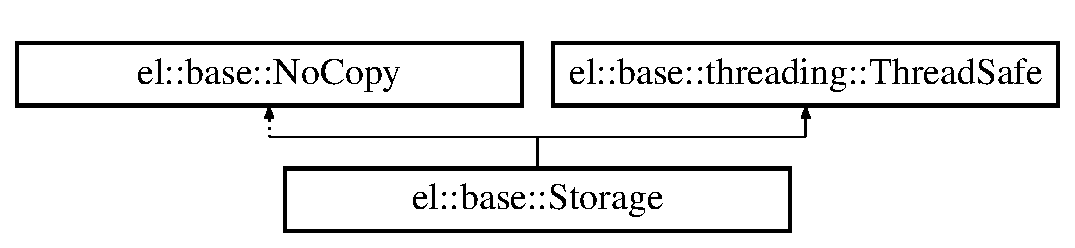
\includegraphics[height=2.000000cm]{classel_1_1base_1_1Storage}
\end{center}
\end{figure}
\subsection*{Public Member Functions}
\begin{DoxyCompactItemize}
\item 
\hypertarget{classel_1_1base_1_1Storage_a4932a8f8a55c3b00467cf2feed6acf59}{{\bfseries Storage} (const Log\-Builder\-Ptr \&default\-Log\-Builder)}\label{classel_1_1base_1_1Storage_a4932a8f8a55c3b00467cf2feed6acf59}

\item 
\hypertarget{classel_1_1base_1_1Storage_a74e5fe30c93b535ee7a1fb20e29bcaf3}{bool {\bfseries validate\-Every\-N\-Counter} (const char $\ast$filename, base\-::type\-::\-Line\-Number line\-Number, std\-::size\-\_\-t occasion)}\label{classel_1_1base_1_1Storage_a74e5fe30c93b535ee7a1fb20e29bcaf3}

\item 
\hypertarget{classel_1_1base_1_1Storage_ad09c13eed65ec6d2248d0693357b1e60}{bool {\bfseries validate\-After\-N\-Counter} (const char $\ast$filename, base\-::type\-::\-Line\-Number line\-Number, std\-::size\-\_\-t n)}\label{classel_1_1base_1_1Storage_ad09c13eed65ec6d2248d0693357b1e60}

\item 
\hypertarget{classel_1_1base_1_1Storage_af6f26975aa70c01ab7f64b2568b2164e}{bool {\bfseries validate\-N\-Times\-Counter} (const char $\ast$filename, base\-::type\-::\-Line\-Number line\-Number, std\-::size\-\_\-t n)}\label{classel_1_1base_1_1Storage_af6f26975aa70c01ab7f64b2568b2164e}

\item 
\hypertarget{classel_1_1base_1_1Storage_accd5495cdad77254eb24ef8f75cd71ad}{\hyperlink{classel_1_1base_1_1RegisteredHitCounters}{base\-::\-Registered\-Hit\-Counters} $\ast$ {\bfseries hit\-Counters} (void) const }\label{classel_1_1base_1_1Storage_accd5495cdad77254eb24ef8f75cd71ad}

\item 
\hypertarget{classel_1_1base_1_1Storage_af0c2f1e119ac3f111f810a324b6b0d3a}{\hyperlink{classel_1_1base_1_1RegisteredLoggers}{base\-::\-Registered\-Loggers} $\ast$ {\bfseries registered\-Loggers} (void) const }\label{classel_1_1base_1_1Storage_af0c2f1e119ac3f111f810a324b6b0d3a}

\item 
\hypertarget{classel_1_1base_1_1Storage_a1ec05ca060ff169569b6ea86da1e30da}{\hyperlink{classel_1_1base_1_1VRegistry}{base\-::\-V\-Registry} $\ast$ {\bfseries v\-Registry} (void) const }\label{classel_1_1base_1_1Storage_a1ec05ca060ff169569b6ea86da1e30da}

\item 
\hypertarget{classel_1_1base_1_1Storage_a84f3d208bead8a8b2c15834be7f30f8d}{const \\*
\hyperlink{classel_1_1base_1_1utils_1_1CommandLineArgs}{base\-::utils\-::\-Command\-Line\-Args} $\ast$ {\bfseries command\-Line\-Args} (void) const }\label{classel_1_1base_1_1Storage_a84f3d208bead8a8b2c15834be7f30f8d}

\item 
\hypertarget{classel_1_1base_1_1Storage_a3e17c61961f3b2f45e8ec77e3320bed5}{void {\bfseries add\-Flag} (\hyperlink{namespaceel_a2784aacd04cb7816ac1c0b20fcbf83cb}{Logging\-Flag} flag)}\label{classel_1_1base_1_1Storage_a3e17c61961f3b2f45e8ec77e3320bed5}

\item 
\hypertarget{classel_1_1base_1_1Storage_aaecbb6ae954d0bf748ac7f3c980a9173}{void {\bfseries remove\-Flag} (\hyperlink{namespaceel_a2784aacd04cb7816ac1c0b20fcbf83cb}{Logging\-Flag} flag)}\label{classel_1_1base_1_1Storage_aaecbb6ae954d0bf748ac7f3c980a9173}

\item 
\hypertarget{classel_1_1base_1_1Storage_ab569cf6e09897b0520dee7f4d1fb742e}{bool {\bfseries has\-Flag} (\hyperlink{namespaceel_a2784aacd04cb7816ac1c0b20fcbf83cb}{Logging\-Flag} flag) const }\label{classel_1_1base_1_1Storage_ab569cf6e09897b0520dee7f4d1fb742e}

\item 
\hypertarget{classel_1_1base_1_1Storage_a0a8da674f034011c50b0479307677855}{base\-::type\-::\-Enum\-Type {\bfseries flags} (void) const }\label{classel_1_1base_1_1Storage_a0a8da674f034011c50b0479307677855}

\item 
\hypertarget{classel_1_1base_1_1Storage_a5df88c56b8d923c20568e50ceb0bdd64}{void {\bfseries set\-Flags} (base\-::type\-::\-Enum\-Type flags)}\label{classel_1_1base_1_1Storage_a5df88c56b8d923c20568e50ceb0bdd64}

\item 
\hypertarget{classel_1_1base_1_1Storage_a626165bc5c8808b733707294ce2a0dc8}{void {\bfseries set\-Pre\-Roll\-Out\-Callback} (const Pre\-Roll\-Out\-Callback \&callback)}\label{classel_1_1base_1_1Storage_a626165bc5c8808b733707294ce2a0dc8}

\item 
\hypertarget{classel_1_1base_1_1Storage_a2bfdc3a20eeafe158ee8603c805131e4}{void {\bfseries unset\-Pre\-Roll\-Out\-Callback} (void)}\label{classel_1_1base_1_1Storage_a2bfdc3a20eeafe158ee8603c805131e4}

\item 
\hypertarget{classel_1_1base_1_1Storage_a90a3a886437746acae51cacbd5731572}{Pre\-Roll\-Out\-Callback \& {\bfseries pre\-Roll\-Out\-Callback} (void)}\label{classel_1_1base_1_1Storage_a90a3a886437746acae51cacbd5731572}

\item 
\hypertarget{classel_1_1base_1_1Storage_ae953cb6e8acafa96c5c1ab2f4826a4a5}{bool {\bfseries has\-Custom\-Format\-Specifier} (const char $\ast$format\-Specifier)}\label{classel_1_1base_1_1Storage_ae953cb6e8acafa96c5c1ab2f4826a4a5}

\item 
\hypertarget{classel_1_1base_1_1Storage_a355aac8191ab98869a52394cc868a315}{void {\bfseries install\-Custom\-Format\-Specifier} (const \hyperlink{classel_1_1CustomFormatSpecifier}{Custom\-Format\-Specifier} \&custom\-Format\-Specifier)}\label{classel_1_1base_1_1Storage_a355aac8191ab98869a52394cc868a315}

\item 
\hypertarget{classel_1_1base_1_1Storage_a68e1d3e0b657418ddb0f62f60fe979d2}{bool {\bfseries uninstall\-Custom\-Format\-Specifier} (const char $\ast$format\-Specifier)}\label{classel_1_1base_1_1Storage_a68e1d3e0b657418ddb0f62f60fe979d2}

\item 
\hypertarget{classel_1_1base_1_1Storage_aaafbc69cac920ec79f60e1cf4c2c12d6}{const std\-::vector\\*
$<$ \hyperlink{classel_1_1CustomFormatSpecifier}{Custom\-Format\-Specifier} $>$ $\ast$ {\bfseries custom\-Format\-Specifiers} (void) const }\label{classel_1_1base_1_1Storage_aaafbc69cac920ec79f60e1cf4c2c12d6}

\item 
\hypertarget{classel_1_1base_1_1Storage_a9f36e06277712a52fd0072f93f068c6f}{\hyperlink{classel_1_1base_1_1threading_1_1internal_1_1NoMutex}{base\-::threading\-::\-Mutex} \& {\bfseries custom\-Format\-Specifiers\-Lock} ()}\label{classel_1_1base_1_1Storage_a9f36e06277712a52fd0072f93f068c6f}

\item 
\hypertarget{classel_1_1base_1_1Storage_a163473357c32184769e8edd993c8b440}{void {\bfseries set\-Logging\-Level} (\hyperlink{namespaceel_ab0ac6091262344c52dd2d3ad099e8e36}{Level} level)}\label{classel_1_1base_1_1Storage_a163473357c32184769e8edd993c8b440}

\item 
\hypertarget{classel_1_1base_1_1Storage_aec36c8e770c0ac354e74d57aba1cfa03}{{\footnotesize template$<$typename T $>$ }\\bool {\bfseries install\-Log\-Dispatch\-Callback} (const std\-::string \&id)}\label{classel_1_1base_1_1Storage_aec36c8e770c0ac354e74d57aba1cfa03}

\item 
\hypertarget{classel_1_1base_1_1Storage_a34c2c9f8abff647e22e1ee0b52357f88}{{\footnotesize template$<$typename T $>$ }\\void {\bfseries uninstall\-Log\-Dispatch\-Callback} (const std\-::string \&id)}\label{classel_1_1base_1_1Storage_a34c2c9f8abff647e22e1ee0b52357f88}

\item 
\hypertarget{classel_1_1base_1_1Storage_a408d2420169a7f7286552fd153967b8d}{{\footnotesize template$<$typename T $>$ }\\T $\ast$ {\bfseries log\-Dispatch\-Callback} (const std\-::string \&id)}\label{classel_1_1base_1_1Storage_a408d2420169a7f7286552fd153967b8d}

\item 
\hypertarget{classel_1_1base_1_1Storage_a1800a786d72b003997dd8d2599b040e0}{void \hyperlink{classel_1_1base_1_1Storage_a1800a786d72b003997dd8d2599b040e0}{set\-Thread\-Name} (const std\-::string \&name)}\label{classel_1_1base_1_1Storage_a1800a786d72b003997dd8d2599b040e0}

\begin{DoxyCompactList}\small\item\em Sets thread name for current thread. Requires std\-::thread. \end{DoxyCompactList}\item 
\hypertarget{classel_1_1base_1_1Storage_aefa8cd1b921eab81d233ae8c5a79f3ee}{std\-::string {\bfseries get\-Thread\-Name} (const std\-::string \&thread\-Id)}\label{classel_1_1base_1_1Storage_aefa8cd1b921eab81d233ae8c5a79f3ee}

\end{DoxyCompactItemize}
\subsection*{Friends}
\begin{DoxyCompactItemize}
\item 
\hypertarget{classel_1_1base_1_1Storage_a2fb8a2c02cbf86247f093c118bed877a}{class {\bfseries el\-::\-Helpers}}\label{classel_1_1base_1_1Storage_a2fb8a2c02cbf86247f093c118bed877a}

\item 
\hypertarget{classel_1_1base_1_1Storage_a42b1de96d584ae4fecbfc2b9aff95052}{class {\bfseries el\-::base\-::\-Default\-Log\-Dispatch\-Callback}}\label{classel_1_1base_1_1Storage_a42b1de96d584ae4fecbfc2b9aff95052}

\item 
\hypertarget{classel_1_1base_1_1Storage_a8c584bcf767a4d007311a7408b22ad62}{class {\bfseries el\-::\-Log\-Builder}}\label{classel_1_1base_1_1Storage_a8c584bcf767a4d007311a7408b22ad62}

\item 
\hypertarget{classel_1_1base_1_1Storage_a81bbf6fe31fab133d182efa8367304f1}{class {\bfseries el\-::base\-::\-Message\-Builder}}\label{classel_1_1base_1_1Storage_a81bbf6fe31fab133d182efa8367304f1}

\item 
\hypertarget{classel_1_1base_1_1Storage_a7a728edbb2761d151832daa74d5b2736}{class {\bfseries el\-::base\-::\-Writer}}\label{classel_1_1base_1_1Storage_a7a728edbb2761d151832daa74d5b2736}

\item 
\hypertarget{classel_1_1base_1_1Storage_a6a4d7851e1984800be3c230f06a79528}{class {\bfseries el\-::base\-::\-Performance\-Tracker}}\label{classel_1_1base_1_1Storage_a6a4d7851e1984800be3c230f06a79528}

\item 
\hypertarget{classel_1_1base_1_1Storage_a9b37b28ea1c5f8f862cc89f135711d92}{class {\bfseries el\-::base\-::\-Log\-Dispatcher}}\label{classel_1_1base_1_1Storage_a9b37b28ea1c5f8f862cc89f135711d92}

\end{DoxyCompactItemize}


\subsection{Detailed Description}
Easylogging++ management storage. 

The documentation for this class was generated from the following file\-:\begin{DoxyCompactItemize}
\item 
/users/disk9/cfse/\-Stage\-\_\-\-Malo/\-C\-P\-A\-C\-S\-Creator\-Lib/\-C\-P\-A\-C\-S\-Creator\-Lib/easylogging++.\-h\end{DoxyCompactItemize}

\hypertarget{classel_1_1base_1_1utils_1_1Str}{\section{el\-:\-:base\-:\-:utils\-:\-:Str Class Reference}
\label{classel_1_1base_1_1utils_1_1Str}\index{el\-::base\-::utils\-::\-Str@{el\-::base\-::utils\-::\-Str}}
}


String utilities helper class used internally. You should not use it.  




{\ttfamily \#include $<$easylogging++.\-h$>$}

Inheritance diagram for el\-:\-:base\-:\-:utils\-:\-:Str\-:\begin{figure}[H]
\begin{center}
\leavevmode
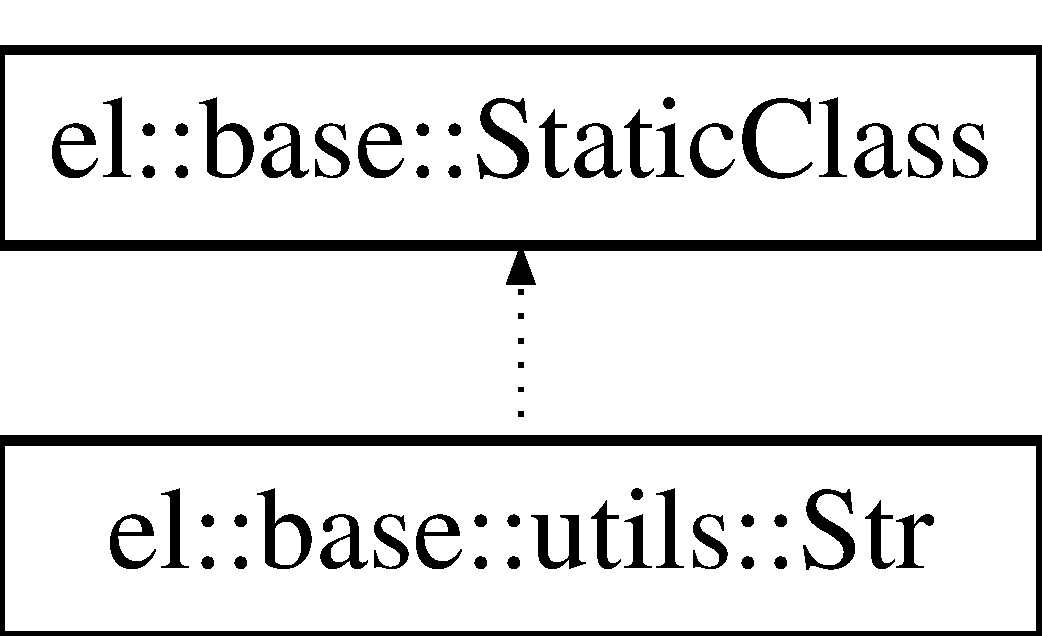
\includegraphics[height=2.000000cm]{classel_1_1base_1_1utils_1_1Str}
\end{center}
\end{figure}
\subsection*{Static Public Member Functions}
\begin{DoxyCompactItemize}
\item 
\hypertarget{classel_1_1base_1_1utils_1_1Str_a4caae91dfe0310d9f182bd9b7e99103c}{static bool \hyperlink{classel_1_1base_1_1utils_1_1Str_a4caae91dfe0310d9f182bd9b7e99103c}{is\-Digit} (char c)}\label{classel_1_1base_1_1utils_1_1Str_a4caae91dfe0310d9f182bd9b7e99103c}

\begin{DoxyCompactList}\small\item\em Checks if character is digit. Dont use libc implementation of it to prevent locale issues. \end{DoxyCompactList}\item 
\hypertarget{classel_1_1base_1_1utils_1_1Str_a95e007a25dfcbd77d4c573b0f73b3153}{static bool \hyperlink{classel_1_1base_1_1utils_1_1Str_a95e007a25dfcbd77d4c573b0f73b3153}{wild\-Card\-Match} (const char $\ast$str, const char $\ast$pattern)}\label{classel_1_1base_1_1utils_1_1Str_a95e007a25dfcbd77d4c573b0f73b3153}

\begin{DoxyCompactList}\small\item\em Matches wildcards, '$\ast$' and '?' only supported. \end{DoxyCompactList}\item 
\hypertarget{classel_1_1base_1_1utils_1_1Str_a64b7a841f04ed916ed8d234b8508703e}{static std\-::string \& {\bfseries ltrim} (std\-::string \&str)}\label{classel_1_1base_1_1utils_1_1Str_a64b7a841f04ed916ed8d234b8508703e}

\item 
\hypertarget{classel_1_1base_1_1utils_1_1Str_a9202797763e10861c4fa84ffd40198bb}{static std\-::string \& {\bfseries rtrim} (std\-::string \&str)}\label{classel_1_1base_1_1utils_1_1Str_a9202797763e10861c4fa84ffd40198bb}

\item 
\hypertarget{classel_1_1base_1_1utils_1_1Str_aba0bc132c410fd3c1e128d1038e996ba}{static std\-::string \& {\bfseries trim} (std\-::string \&str)}\label{classel_1_1base_1_1utils_1_1Str_aba0bc132c410fd3c1e128d1038e996ba}

\item 
static bool \hyperlink{classel_1_1base_1_1utils_1_1Str_acf80221cec72da701ef50995a61ab91f}{starts\-With} (const std\-::string \&str, const std\-::string \&start)
\begin{DoxyCompactList}\small\item\em Determines whether or not str starts with specified string. \end{DoxyCompactList}\item 
static bool \hyperlink{classel_1_1base_1_1utils_1_1Str_a5bcf5f6cc41a7ed683be115148579561}{ends\-With} (const std\-::string \&str, const std\-::string \&end)
\begin{DoxyCompactList}\small\item\em Determines whether or not str ends with specified string. \end{DoxyCompactList}\item 
static std\-::string \& \hyperlink{classel_1_1base_1_1utils_1_1Str_aa07bfda259ed194120b371401734ae86}{replace\-All} (std\-::string \&str, char replace\-What, char replace\-With)
\begin{DoxyCompactList}\small\item\em Replaces all instances of replace\-What with 'replace\-With'. Original variable is changed for performance. \end{DoxyCompactList}\item 
static std\-::string \& \hyperlink{classel_1_1base_1_1utils_1_1Str_a8e823aa60b160451ca0b8732c3c75568}{replace\-All} (std\-::string \&str, const std\-::string \&replace\-What, const std\-::string \&replace\-With)
\begin{DoxyCompactList}\small\item\em Replaces all instances of 'replace\-What' with 'replace\-With'. (String version) Replaces in place. \end{DoxyCompactList}\item 
\hypertarget{classel_1_1base_1_1utils_1_1Str_a3725349f601d07316d1c2bc211daaaa1}{static void {\bfseries replace\-First\-With\-Escape} (base\-::type\-::string\-\_\-t \&str, const base\-::type\-::string\-\_\-t \&replace\-What, const base\-::type\-::string\-\_\-t \&replace\-With)}\label{classel_1_1base_1_1utils_1_1Str_a3725349f601d07316d1c2bc211daaaa1}

\item 
static std\-::string \& \hyperlink{classel_1_1base_1_1utils_1_1Str_a6a05315fb967508dc1faf0584421a95d}{to\-Upper} (std\-::string \&str)
\begin{DoxyCompactList}\small\item\em Converts string to uppercase. \end{DoxyCompactList}\item 
\hypertarget{classel_1_1base_1_1utils_1_1Str_a8081458c7848ff991d765c69f7858c44}{static bool \hyperlink{classel_1_1base_1_1utils_1_1Str_a8081458c7848ff991d765c69f7858c44}{c\-String\-Eq} (const char $\ast$s1, const char $\ast$s2)}\label{classel_1_1base_1_1utils_1_1Str_a8081458c7848ff991d765c69f7858c44}

\begin{DoxyCompactList}\small\item\em Compares cstring equality -\/ uses strcmp. \end{DoxyCompactList}\item 
\hypertarget{classel_1_1base_1_1utils_1_1Str_aaa37755d713b5e6475950134ce9ce0e8}{static bool \hyperlink{classel_1_1base_1_1utils_1_1Str_aaa37755d713b5e6475950134ce9ce0e8}{c\-String\-Case\-Eq} (const char $\ast$s1, const char $\ast$s2)}\label{classel_1_1base_1_1utils_1_1Str_aaa37755d713b5e6475950134ce9ce0e8}

\begin{DoxyCompactList}\small\item\em Compares cstring equality (case-\/insensitive) -\/ uses toupper(char) Dont use strcasecmp because of C\-R\-T (V\-C++) \end{DoxyCompactList}\item 
\hypertarget{classel_1_1base_1_1utils_1_1Str_a27cc1c1625b21597eb75df62b8fca0f8}{static bool \hyperlink{classel_1_1base_1_1utils_1_1Str_a27cc1c1625b21597eb75df62b8fca0f8}{contains} (const char $\ast$str, char c)}\label{classel_1_1base_1_1utils_1_1Str_a27cc1c1625b21597eb75df62b8fca0f8}

\begin{DoxyCompactList}\small\item\em Returns true if c exist in str. \end{DoxyCompactList}\item 
\hypertarget{classel_1_1base_1_1utils_1_1Str_a5e12c163bf1085441ea5453fd6c62fa0}{static char $\ast$ {\bfseries convert\-And\-Add\-To\-Buff} (std\-::size\-\_\-t n, int len, char $\ast$buf, const char $\ast$buf\-Lim, bool zero\-Padded=true)}\label{classel_1_1base_1_1utils_1_1Str_a5e12c163bf1085441ea5453fd6c62fa0}

\item 
\hypertarget{classel_1_1base_1_1utils_1_1Str_aa6a96f625f71661c02ecd5366533abaa}{static char $\ast$ {\bfseries add\-To\-Buff} (const char $\ast$str, char $\ast$buf, const char $\ast$buf\-Lim)}\label{classel_1_1base_1_1utils_1_1Str_aa6a96f625f71661c02ecd5366533abaa}

\item 
\hypertarget{classel_1_1base_1_1utils_1_1Str_adf0c36c9b8276ede18111a866e31db8b}{static char $\ast$ {\bfseries clear\-Buff} (char buff\mbox{[}$\,$\mbox{]}, std\-::size\-\_\-t lim)}\label{classel_1_1base_1_1utils_1_1Str_adf0c36c9b8276ede18111a866e31db8b}

\item 
\hypertarget{classel_1_1base_1_1utils_1_1Str_a6dc022e7e8d4cbf2c80ba9e1354feaea}{static char $\ast$ \hyperlink{classel_1_1base_1_1utils_1_1Str_a6dc022e7e8d4cbf2c80ba9e1354feaea}{wchar\-Ptr\-To\-Char\-Ptr} (const wchar\-\_\-t $\ast$line)}\label{classel_1_1base_1_1utils_1_1Str_a6dc022e7e8d4cbf2c80ba9e1354feaea}

\begin{DoxyCompactList}\small\item\em Converst wchar$\ast$ to char$\ast$ N\-O\-T\-E\-: Need to free return value after use! \end{DoxyCompactList}\end{DoxyCompactItemize}


\subsection{Detailed Description}
String utilities helper class used internally. You should not use it. 

\subsection{Member Function Documentation}
\hypertarget{classel_1_1base_1_1utils_1_1Str_a5bcf5f6cc41a7ed683be115148579561}{\index{el\-::base\-::utils\-::\-Str@{el\-::base\-::utils\-::\-Str}!ends\-With@{ends\-With}}
\index{ends\-With@{ends\-With}!el::base::utils::Str@{el\-::base\-::utils\-::\-Str}}
\subsubsection[{ends\-With}]{\setlength{\rightskip}{0pt plus 5cm}static bool el\-::base\-::utils\-::\-Str\-::ends\-With (
\begin{DoxyParamCaption}
\item[{const std\-::string \&}]{str, }
\item[{const std\-::string \&}]{end}
\end{DoxyParamCaption}
)\hspace{0.3cm}{\ttfamily [static]}}}\label{classel_1_1base_1_1utils_1_1Str_a5bcf5f6cc41a7ed683be115148579561}


Determines whether or not str ends with specified string. 


\begin{DoxyParams}{Parameters}
{\em str} & String to check \\
\hline
{\em end} & String to check against \\
\hline
\end{DoxyParams}
\begin{DoxyReturn}{Returns}
Returns true if ends with specified string, false otherwise 
\end{DoxyReturn}
\hypertarget{classel_1_1base_1_1utils_1_1Str_aa07bfda259ed194120b371401734ae86}{\index{el\-::base\-::utils\-::\-Str@{el\-::base\-::utils\-::\-Str}!replace\-All@{replace\-All}}
\index{replace\-All@{replace\-All}!el::base::utils::Str@{el\-::base\-::utils\-::\-Str}}
\subsubsection[{replace\-All}]{\setlength{\rightskip}{0pt plus 5cm}static std\-::string\& el\-::base\-::utils\-::\-Str\-::replace\-All (
\begin{DoxyParamCaption}
\item[{std\-::string \&}]{str, }
\item[{char}]{replace\-What, }
\item[{char}]{replace\-With}
\end{DoxyParamCaption}
)\hspace{0.3cm}{\ttfamily [static]}}}\label{classel_1_1base_1_1utils_1_1Str_aa07bfda259ed194120b371401734ae86}


Replaces all instances of replace\-What with 'replace\-With'. Original variable is changed for performance. 


\begin{DoxyParams}[1]{Parameters}
\mbox{\tt in,out}  & {\em str} & String to replace from \\
\hline
 & {\em replace\-What} & Character to replace \\
\hline
 & {\em replace\-With} & Character to replace with \\
\hline
\end{DoxyParams}
\begin{DoxyReturn}{Returns}
Modified version of str 
\end{DoxyReturn}
\hypertarget{classel_1_1base_1_1utils_1_1Str_a8e823aa60b160451ca0b8732c3c75568}{\index{el\-::base\-::utils\-::\-Str@{el\-::base\-::utils\-::\-Str}!replace\-All@{replace\-All}}
\index{replace\-All@{replace\-All}!el::base::utils::Str@{el\-::base\-::utils\-::\-Str}}
\subsubsection[{replace\-All}]{\setlength{\rightskip}{0pt plus 5cm}static std\-::string\& el\-::base\-::utils\-::\-Str\-::replace\-All (
\begin{DoxyParamCaption}
\item[{std\-::string \&}]{str, }
\item[{const std\-::string \&}]{replace\-What, }
\item[{const std\-::string \&}]{replace\-With}
\end{DoxyParamCaption}
)\hspace{0.3cm}{\ttfamily [static]}}}\label{classel_1_1base_1_1utils_1_1Str_a8e823aa60b160451ca0b8732c3c75568}


Replaces all instances of 'replace\-What' with 'replace\-With'. (String version) Replaces in place. 


\begin{DoxyParams}{Parameters}
{\em str} & String to replace from \\
\hline
{\em replace\-What} & Character to replace \\
\hline
{\em replace\-With} & Character to replace with \\
\hline
\end{DoxyParams}
\begin{DoxyReturn}{Returns}
Modified (original) str 
\end{DoxyReturn}
\hypertarget{classel_1_1base_1_1utils_1_1Str_acf80221cec72da701ef50995a61ab91f}{\index{el\-::base\-::utils\-::\-Str@{el\-::base\-::utils\-::\-Str}!starts\-With@{starts\-With}}
\index{starts\-With@{starts\-With}!el::base::utils::Str@{el\-::base\-::utils\-::\-Str}}
\subsubsection[{starts\-With}]{\setlength{\rightskip}{0pt plus 5cm}static bool el\-::base\-::utils\-::\-Str\-::starts\-With (
\begin{DoxyParamCaption}
\item[{const std\-::string \&}]{str, }
\item[{const std\-::string \&}]{start}
\end{DoxyParamCaption}
)\hspace{0.3cm}{\ttfamily [static]}}}\label{classel_1_1base_1_1utils_1_1Str_acf80221cec72da701ef50995a61ab91f}


Determines whether or not str starts with specified string. 


\begin{DoxyParams}{Parameters}
{\em str} & String to check \\
\hline
{\em start} & String to check against \\
\hline
\end{DoxyParams}
\begin{DoxyReturn}{Returns}
Returns true if starts with specified string, false otherwise 
\end{DoxyReturn}
\hypertarget{classel_1_1base_1_1utils_1_1Str_a6a05315fb967508dc1faf0584421a95d}{\index{el\-::base\-::utils\-::\-Str@{el\-::base\-::utils\-::\-Str}!to\-Upper@{to\-Upper}}
\index{to\-Upper@{to\-Upper}!el::base::utils::Str@{el\-::base\-::utils\-::\-Str}}
\subsubsection[{to\-Upper}]{\setlength{\rightskip}{0pt plus 5cm}static std\-::string\& el\-::base\-::utils\-::\-Str\-::to\-Upper (
\begin{DoxyParamCaption}
\item[{std\-::string \&}]{str}
\end{DoxyParamCaption}
)\hspace{0.3cm}{\ttfamily [static]}}}\label{classel_1_1base_1_1utils_1_1Str_a6a05315fb967508dc1faf0584421a95d}


Converts string to uppercase. 


\begin{DoxyParams}{Parameters}
{\em str} & String to convert \\
\hline
\end{DoxyParams}
\begin{DoxyReturn}{Returns}
Uppercase string 
\end{DoxyReturn}


The documentation for this class was generated from the following file\-:\begin{DoxyCompactItemize}
\item 
/users/disk9/cfse/\-Stage\-\_\-\-Malo/\-C\-P\-A\-C\-S\-Creator\-Lib/\-C\-P\-A\-C\-S\-Creator\-Lib/easylogging++.\-h\end{DoxyCompactItemize}

\hypertarget{classel_1_1base_1_1SubsecondPrecision}{\section{el\-:\-:base\-:\-:Subsecond\-Precision Class Reference}
\label{classel_1_1base_1_1SubsecondPrecision}\index{el\-::base\-::\-Subsecond\-Precision@{el\-::base\-::\-Subsecond\-Precision}}
}


A subsecond precision class containing actual width and offset of the subsecond part.  




{\ttfamily \#include $<$easylogging++.\-h$>$}

\subsection*{Public Member Functions}
\begin{DoxyCompactItemize}
\item 
\hypertarget{classel_1_1base_1_1SubsecondPrecision_aff4556f058704e26df60907bf95998ff}{{\bfseries Subsecond\-Precision} (int width)}\label{classel_1_1base_1_1SubsecondPrecision_aff4556f058704e26df60907bf95998ff}

\item 
\hypertarget{classel_1_1base_1_1SubsecondPrecision_a5bb2fe83619b7007aac61252e4dc5186}{bool {\bfseries operator==} (const \hyperlink{classel_1_1base_1_1SubsecondPrecision}{Subsecond\-Precision} \&ss\-Prec)}\label{classel_1_1base_1_1SubsecondPrecision_a5bb2fe83619b7007aac61252e4dc5186}

\end{DoxyCompactItemize}
\subsection*{Public Attributes}
\begin{DoxyCompactItemize}
\item 
\hypertarget{classel_1_1base_1_1SubsecondPrecision_a7e24991325599de4d9ff96ac691cbbf6}{int {\bfseries m\-\_\-width}}\label{classel_1_1base_1_1SubsecondPrecision_a7e24991325599de4d9ff96ac691cbbf6}

\item 
\hypertarget{classel_1_1base_1_1SubsecondPrecision_a3d14e3d57e57e799d105f7b86d190dcf}{unsigned int {\bfseries m\-\_\-offset}}\label{classel_1_1base_1_1SubsecondPrecision_a3d14e3d57e57e799d105f7b86d190dcf}

\end{DoxyCompactItemize}


\subsection{Detailed Description}
A subsecond precision class containing actual width and offset of the subsecond part. 

The documentation for this class was generated from the following file\-:\begin{DoxyCompactItemize}
\item 
/users/disk9/cfse/\-Stage\-\_\-\-Malo/\-C\-P\-A\-C\-S\-Creator\-Lib/\-C\-P\-A\-C\-S\-Creator\-Lib/easylogging++.\-h\end{DoxyCompactItemize}

\hypertarget{classel_1_1SysLogInitializer}{\section{el\-:\-:Sys\-Log\-Initializer Class Reference}
\label{classel_1_1SysLogInitializer}\index{el\-::\-Sys\-Log\-Initializer@{el\-::\-Sys\-Log\-Initializer}}
}


Initializes syslog with process I\-D, options and facility. calls closelog() on d'tor.  




{\ttfamily \#include $<$easylogging++.\-h$>$}

\subsection*{Public Member Functions}
\begin{DoxyCompactItemize}
\item 
\hypertarget{classel_1_1SysLogInitializer_aae71ee83f45c4cf770fbc6c6e87d9406}{{\bfseries Sys\-Log\-Initializer} (const char $\ast$process\-Ident, int options=0, int facility=0)}\label{classel_1_1SysLogInitializer_aae71ee83f45c4cf770fbc6c6e87d9406}

\end{DoxyCompactItemize}


\subsection{Detailed Description}
Initializes syslog with process I\-D, options and facility. calls closelog() on d'tor. 

The documentation for this class was generated from the following file\-:\begin{DoxyCompactItemize}
\item 
/users/disk9/cfse/\-Stage\-\_\-\-Malo/\-C\-P\-A\-C\-S\-Creator\-Lib/\-C\-P\-A\-C\-S\-Creator\-Lib/easylogging++.\-h\end{DoxyCompactItemize}

\hypertarget{classel_1_1base_1_1threading_1_1ThreadSafe}{\section{el\-:\-:base\-:\-:threading\-:\-:Thread\-Safe Class Reference}
\label{classel_1_1base_1_1threading_1_1ThreadSafe}\index{el\-::base\-::threading\-::\-Thread\-Safe@{el\-::base\-::threading\-::\-Thread\-Safe}}
}


Base of thread safe class, this class is inheritable-\/only.  




{\ttfamily \#include $<$easylogging++.\-h$>$}

Inheritance diagram for el\-:\-:base\-:\-:threading\-:\-:Thread\-Safe\-:\begin{figure}[H]
\begin{center}
\leavevmode
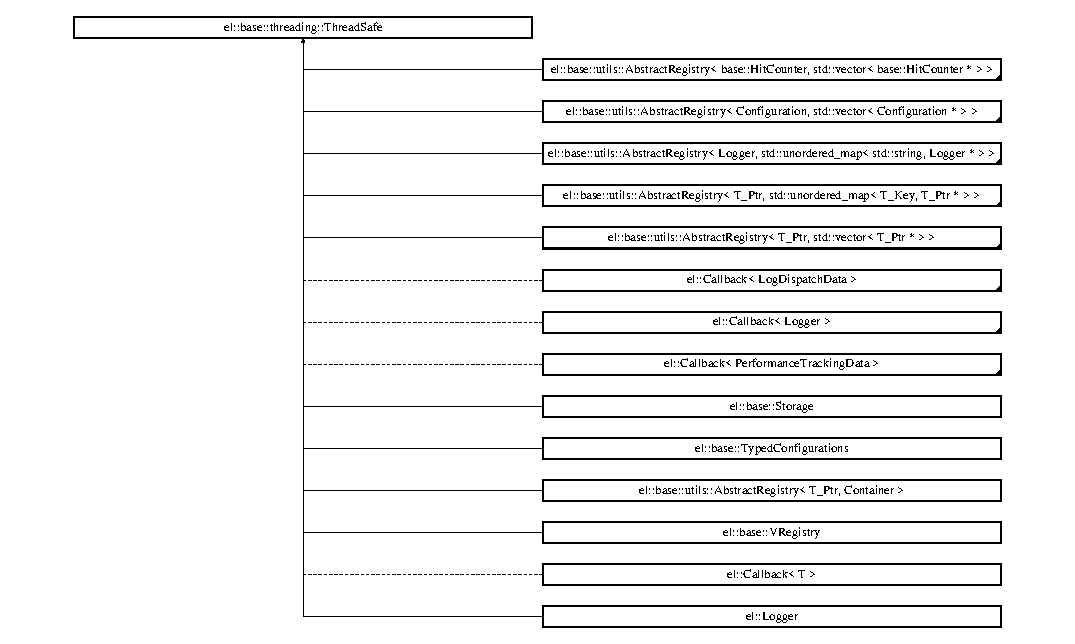
\includegraphics[height=8.203125cm]{classel_1_1base_1_1threading_1_1ThreadSafe}
\end{center}
\end{figure}
\subsection*{Public Member Functions}
\begin{DoxyCompactItemize}
\item 
\hypertarget{classel_1_1base_1_1threading_1_1ThreadSafe_a59db719b214f7118f0919846a85077bf}{virtual void {\bfseries acquire\-Lock} (void) E\-L\-P\-P\-\_\-\-F\-I\-N\-A\-L}\label{classel_1_1base_1_1threading_1_1ThreadSafe_a59db719b214f7118f0919846a85077bf}

\item 
\hypertarget{classel_1_1base_1_1threading_1_1ThreadSafe_a95bb166242b9691f861274a9b8ced2d9}{virtual void {\bfseries release\-Lock} (void) E\-L\-P\-P\-\_\-\-F\-I\-N\-A\-L}\label{classel_1_1base_1_1threading_1_1ThreadSafe_a95bb166242b9691f861274a9b8ced2d9}

\item 
\hypertarget{classel_1_1base_1_1threading_1_1ThreadSafe_affb45b35790a7305d0a659562c8104fc}{virtual \hyperlink{classel_1_1base_1_1threading_1_1internal_1_1NoMutex}{base\-::threading\-::\-Mutex} \& {\bfseries lock} (void) E\-L\-P\-P\-\_\-\-F\-I\-N\-A\-L}\label{classel_1_1base_1_1threading_1_1ThreadSafe_affb45b35790a7305d0a659562c8104fc}

\end{DoxyCompactItemize}


\subsection{Detailed Description}
Base of thread safe class, this class is inheritable-\/only. 

The documentation for this class was generated from the following file\-:\begin{DoxyCompactItemize}
\item 
/users/disk9/cfse/\-Stage\-\_\-\-Malo/\-C\-P\-A\-C\-S\-Creator\-Lib/\-C\-P\-A\-C\-S\-Creator\-Lib/easylogging++.\-h\end{DoxyCompactItemize}

\hypertarget{classel_1_1base_1_1TypedConfigurations}{\section{el\-:\-:base\-:\-:Typed\-Configurations Class Reference}
\label{classel_1_1base_1_1TypedConfigurations}\index{el\-::base\-::\-Typed\-Configurations@{el\-::base\-::\-Typed\-Configurations}}
}


\hyperlink{classel_1_1Configurations}{Configurations} with data types.  




{\ttfamily \#include $<$easylogging++.\-h$>$}

Inheritance diagram for el\-:\-:base\-:\-:Typed\-Configurations\-:\begin{figure}[H]
\begin{center}
\leavevmode
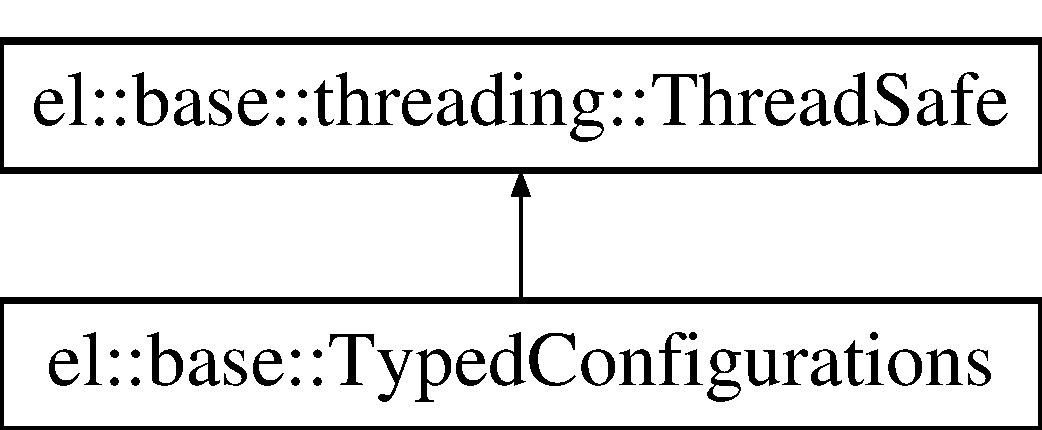
\includegraphics[height=2.000000cm]{classel_1_1base_1_1TypedConfigurations}
\end{center}
\end{figure}
\subsection*{Public Member Functions}
\begin{DoxyCompactItemize}
\item 
\hyperlink{classel_1_1base_1_1TypedConfigurations_a1b6d90479bb79da27c3e351a9be593ae}{Typed\-Configurations} (\hyperlink{classel_1_1Configurations}{Configurations} $\ast$configurations, base\-::\-Log\-Streams\-Reference\-Map $\ast$log\-Streams\-Reference)
\begin{DoxyCompactList}\small\item\em Constructor to initialize (construct) the object off \hyperlink{classel_1_1Configurations}{el\-::\-Configurations}. \end{DoxyCompactList}\item 
\hypertarget{classel_1_1base_1_1TypedConfigurations_ae7b346e5d32305d4957bc6c564409090}{{\bfseries Typed\-Configurations} (const \hyperlink{classel_1_1base_1_1TypedConfigurations}{Typed\-Configurations} \&other)}\label{classel_1_1base_1_1TypedConfigurations_ae7b346e5d32305d4957bc6c564409090}

\item 
\hypertarget{classel_1_1base_1_1TypedConfigurations_a65d2ec91ff7edc07db304ebd9c30291f}{const \hyperlink{classel_1_1Configurations}{Configurations} $\ast$ {\bfseries configurations} (void) const }\label{classel_1_1base_1_1TypedConfigurations_a65d2ec91ff7edc07db304ebd9c30291f}

\item 
\hypertarget{classel_1_1base_1_1TypedConfigurations_a924b35df988103c737907cc7993c3c1c}{bool {\bfseries enabled} (\hyperlink{namespaceel_ab0ac6091262344c52dd2d3ad099e8e36}{Level} level)}\label{classel_1_1base_1_1TypedConfigurations_a924b35df988103c737907cc7993c3c1c}

\item 
\hypertarget{classel_1_1base_1_1TypedConfigurations_a20b9a1bd152cad3b72b558f97de3876b}{bool {\bfseries to\-File} (\hyperlink{namespaceel_ab0ac6091262344c52dd2d3ad099e8e36}{Level} level)}\label{classel_1_1base_1_1TypedConfigurations_a20b9a1bd152cad3b72b558f97de3876b}

\item 
\hypertarget{classel_1_1base_1_1TypedConfigurations_a6a7871c0c37c3306334e90dfdc1d2e47}{const std\-::string \& {\bfseries filename} (\hyperlink{namespaceel_ab0ac6091262344c52dd2d3ad099e8e36}{Level} level)}\label{classel_1_1base_1_1TypedConfigurations_a6a7871c0c37c3306334e90dfdc1d2e47}

\item 
\hypertarget{classel_1_1base_1_1TypedConfigurations_aeaa7bf7448319bc41e4e226124288c7e}{bool {\bfseries to\-Standard\-Output} (\hyperlink{namespaceel_ab0ac6091262344c52dd2d3ad099e8e36}{Level} level)}\label{classel_1_1base_1_1TypedConfigurations_aeaa7bf7448319bc41e4e226124288c7e}

\item 
\hypertarget{classel_1_1base_1_1TypedConfigurations_a5d4d84a3dda6d54e0f291917703db441}{const \hyperlink{classel_1_1base_1_1LogFormat}{base\-::\-Log\-Format} \& {\bfseries log\-Format} (\hyperlink{namespaceel_ab0ac6091262344c52dd2d3ad099e8e36}{Level} level)}\label{classel_1_1base_1_1TypedConfigurations_a5d4d84a3dda6d54e0f291917703db441}

\item 
\hypertarget{classel_1_1base_1_1TypedConfigurations_a983b96fb732ed1d9d7f515dc81090daa}{const \hyperlink{classel_1_1base_1_1SubsecondPrecision}{base\-::\-Subsecond\-Precision} \& {\bfseries subsecond\-Precision} (\hyperlink{namespaceel_ab0ac6091262344c52dd2d3ad099e8e36}{Level} level=\hyperlink{namespaceel_ab0ac6091262344c52dd2d3ad099e8e36a4cc6684df7b4a92b1dec6fce3264fac8}{Level\-::\-Global})}\label{classel_1_1base_1_1TypedConfigurations_a983b96fb732ed1d9d7f515dc81090daa}

\item 
\hypertarget{classel_1_1base_1_1TypedConfigurations_ad078669014b01e587987e9ffc2214763}{const \hyperlink{namespaceel_1_1base_abbc234f4907eccec2673dfc6efaa5925}{base\-::\-Milliseconds\-Width} \& {\bfseries milliseconds\-Width} (\hyperlink{namespaceel_ab0ac6091262344c52dd2d3ad099e8e36}{Level} level=\hyperlink{namespaceel_ab0ac6091262344c52dd2d3ad099e8e36a4cc6684df7b4a92b1dec6fce3264fac8}{Level\-::\-Global})}\label{classel_1_1base_1_1TypedConfigurations_ad078669014b01e587987e9ffc2214763}

\item 
\hypertarget{classel_1_1base_1_1TypedConfigurations_a0cef785df86dbfe17a27c5b78ed3e5da}{bool {\bfseries performance\-Tracking} (\hyperlink{namespaceel_ab0ac6091262344c52dd2d3ad099e8e36}{Level} level=\hyperlink{namespaceel_ab0ac6091262344c52dd2d3ad099e8e36a4cc6684df7b4a92b1dec6fce3264fac8}{Level\-::\-Global})}\label{classel_1_1base_1_1TypedConfigurations_a0cef785df86dbfe17a27c5b78ed3e5da}

\item 
\hypertarget{classel_1_1base_1_1TypedConfigurations_abb8250bc165b182524521faef6bedb19}{base\-::type\-::fstream\-\_\-t $\ast$ {\bfseries file\-Stream} (\hyperlink{namespaceel_ab0ac6091262344c52dd2d3ad099e8e36}{Level} level)}\label{classel_1_1base_1_1TypedConfigurations_abb8250bc165b182524521faef6bedb19}

\item 
\hypertarget{classel_1_1base_1_1TypedConfigurations_aa48c0568be8fd177f1d463b1e7831f75}{std\-::size\-\_\-t {\bfseries max\-Log\-File\-Size} (\hyperlink{namespaceel_ab0ac6091262344c52dd2d3ad099e8e36}{Level} level)}\label{classel_1_1base_1_1TypedConfigurations_aa48c0568be8fd177f1d463b1e7831f75}

\item 
\hypertarget{classel_1_1base_1_1TypedConfigurations_ae8710257d7f8bc20c2183a3a4404ebaf}{std\-::size\-\_\-t {\bfseries log\-Flush\-Threshold} (\hyperlink{namespaceel_ab0ac6091262344c52dd2d3ad099e8e36}{Level} level)}\label{classel_1_1base_1_1TypedConfigurations_ae8710257d7f8bc20c2183a3a4404ebaf}

\end{DoxyCompactItemize}
\subsection*{Friends}
\begin{DoxyCompactItemize}
\item 
\hypertarget{classel_1_1base_1_1TypedConfigurations_a2fb8a2c02cbf86247f093c118bed877a}{class {\bfseries el\-::\-Helpers}}\label{classel_1_1base_1_1TypedConfigurations_a2fb8a2c02cbf86247f093c118bed877a}

\item 
\hypertarget{classel_1_1base_1_1TypedConfigurations_a81bbf6fe31fab133d182efa8367304f1}{class {\bfseries el\-::base\-::\-Message\-Builder}}\label{classel_1_1base_1_1TypedConfigurations_a81bbf6fe31fab133d182efa8367304f1}

\item 
\hypertarget{classel_1_1base_1_1TypedConfigurations_a7a728edbb2761d151832daa74d5b2736}{class {\bfseries el\-::base\-::\-Writer}}\label{classel_1_1base_1_1TypedConfigurations_a7a728edbb2761d151832daa74d5b2736}

\item 
\hypertarget{classel_1_1base_1_1TypedConfigurations_a42b1de96d584ae4fecbfc2b9aff95052}{class {\bfseries el\-::base\-::\-Default\-Log\-Dispatch\-Callback}}\label{classel_1_1base_1_1TypedConfigurations_a42b1de96d584ae4fecbfc2b9aff95052}

\item 
\hypertarget{classel_1_1base_1_1TypedConfigurations_a9b37b28ea1c5f8f862cc89f135711d92}{class {\bfseries el\-::base\-::\-Log\-Dispatcher}}\label{classel_1_1base_1_1TypedConfigurations_a9b37b28ea1c5f8f862cc89f135711d92}

\end{DoxyCompactItemize}


\subsection{Detailed Description}
\hyperlink{classel_1_1Configurations}{Configurations} with data types. 

\hyperlink{classel_1_1Configurations}{el\-::\-Configurations} have string based values. This is whats used internally in order to read correct configurations. This is to perform faster while writing logs using correct configurations.

This is thread safe and final class containing non-\/virtual destructor (means nothing should inherit this class) 

\subsection{Constructor \& Destructor Documentation}
\hypertarget{classel_1_1base_1_1TypedConfigurations_a1b6d90479bb79da27c3e351a9be593ae}{\index{el\-::base\-::\-Typed\-Configurations@{el\-::base\-::\-Typed\-Configurations}!Typed\-Configurations@{Typed\-Configurations}}
\index{Typed\-Configurations@{Typed\-Configurations}!el::base::TypedConfigurations@{el\-::base\-::\-Typed\-Configurations}}
\subsubsection[{Typed\-Configurations}]{\setlength{\rightskip}{0pt plus 5cm}el\-::base\-::\-Typed\-Configurations\-::\-Typed\-Configurations (
\begin{DoxyParamCaption}
\item[{{\bf Configurations} $\ast$}]{configurations, }
\item[{base\-::\-Log\-Streams\-Reference\-Map $\ast$}]{log\-Streams\-Reference}
\end{DoxyParamCaption}
)}}\label{classel_1_1base_1_1TypedConfigurations_a1b6d90479bb79da27c3e351a9be593ae}


Constructor to initialize (construct) the object off \hyperlink{classel_1_1Configurations}{el\-::\-Configurations}. 


\begin{DoxyParams}{Parameters}
{\em configurations} & \hyperlink{classel_1_1Configurations}{Configurations} pointer/reference to base this typed configurations off. \\
\hline
{\em log\-Streams\-Reference} & Use E\-L\-P\-P-\/$>$registered\-Loggers()-\/$>$log\-Streams\-Reference() \\
\hline
\end{DoxyParams}


The documentation for this class was generated from the following file\-:\begin{DoxyCompactItemize}
\item 
/users/disk9/cfse/\-Stage\-\_\-\-Malo/\-C\-P\-A\-C\-S\-Creator\-Lib/\-C\-P\-A\-C\-S\-Creator\-Lib/easylogging++.\-h\end{DoxyCompactItemize}

\hypertarget{classcpcr_1_1UniqueXPath}{\section{cpcr\-:\-:Unique\-X\-Path Class Reference}
\label{classcpcr_1_1UniqueXPath}\index{cpcr\-::\-Unique\-X\-Path@{cpcr\-::\-Unique\-X\-Path}}
}
\subsection*{Public Member Functions}
\begin{DoxyCompactItemize}
\item 
\hypertarget{classcpcr_1_1UniqueXPath_a486e85db63833a0ca1891a3ad5b3ed69}{{\bfseries Unique\-X\-Path} (std\-::string x)}\label{classcpcr_1_1UniqueXPath_a486e85db63833a0ca1891a3ad5b3ed69}

\item 
\hypertarget{classcpcr_1_1UniqueXPath_ae89e000a7b5f95547ca6ad0c94ef442c}{bool {\bfseries is\-Empty} () const }\label{classcpcr_1_1UniqueXPath_ae89e000a7b5f95547ca6ad0c94ef442c}

\item 
\hypertarget{classcpcr_1_1UniqueXPath_a372eb1a34a1f8404eab45bc528e6bf52}{std\-::string {\bfseries to\-String} () const }\label{classcpcr_1_1UniqueXPath_a372eb1a34a1f8404eab45bc528e6bf52}

\item 
\hypertarget{classcpcr_1_1UniqueXPath_a7951602556af4adf8d92b03366b4061a}{void {\bfseries set\-X\-Path} (std\-::string new\-X\-Path)}\label{classcpcr_1_1UniqueXPath_a7951602556af4adf8d92b03366b4061a}

\item 
\hypertarget{classcpcr_1_1UniqueXPath_a4e2ebbcb2a962d01bf59fdb6f7bfed70}{void {\bfseries add\-Particle\-At\-End} (std\-::string particle)}\label{classcpcr_1_1UniqueXPath_a4e2ebbcb2a962d01bf59fdb6f7bfed70}

\item 
\hypertarget{classcpcr_1_1UniqueXPath_aebba576085cd3bc1675a6be8b2b1f189}{std\-::string {\bfseries get\-First\-Element\-Type} () const }\label{classcpcr_1_1UniqueXPath_aebba576085cd3bc1675a6be8b2b1f189}

\item 
\hypertarget{classcpcr_1_1UniqueXPath_ae17acff34b7cad0ac44b645ceeef7152}{std\-::string {\bfseries get\-Last\-Element\-Type} () const }\label{classcpcr_1_1UniqueXPath_ae17acff34b7cad0ac44b645ceeef7152}

\item 
\hypertarget{classcpcr_1_1UniqueXPath_a020206007546296ec095c5d28f482331}{int {\bfseries get\-First\-Element\-Index} () const }\label{classcpcr_1_1UniqueXPath_a020206007546296ec095c5d28f482331}

\item 
\hypertarget{classcpcr_1_1UniqueXPath_a02fb1823fa77eadd30ff65effedeb848}{int {\bfseries get\-Last\-Element\-Index} () const }\label{classcpcr_1_1UniqueXPath_a02fb1823fa77eadd30ff65effedeb848}

\item 
\hypertarget{classcpcr_1_1UniqueXPath_a0e48bccef51b3d862cd1f417d693354c}{std\-::string {\bfseries pop\-First} ()}\label{classcpcr_1_1UniqueXPath_a0e48bccef51b3d862cd1f417d693354c}

\item 
\hypertarget{classcpcr_1_1UniqueXPath_a34fa02c1c9ada5c3552dfd52202f1d2c}{std\-::string {\bfseries pop\-Last} ()}\label{classcpcr_1_1UniqueXPath_a34fa02c1c9ada5c3552dfd52202f1d2c}

\item 
\hypertarget{classcpcr_1_1UniqueXPath_a55e46de7c69a31bbea4fdb75c11b10e5}{\hyperlink{classcpcr_1_1UniqueXPath}{Unique\-X\-Path} {\bfseries relative\-To} (const \hyperlink{classcpcr_1_1UniqueXPath}{Unique\-X\-Path} \&other)}\label{classcpcr_1_1UniqueXPath_a55e46de7c69a31bbea4fdb75c11b10e5}

\item 
\hypertarget{classcpcr_1_1UniqueXPath_a15e27236ee99ef737e976954377ea40c}{bool {\bfseries operator==} (const \hyperlink{classcpcr_1_1UniqueXPath}{Unique\-X\-Path} \&other)}\label{classcpcr_1_1UniqueXPath_a15e27236ee99ef737e976954377ea40c}

\item 
\hypertarget{classcpcr_1_1UniqueXPath_ac1c0c8f241ee5e60cb68d1799930220d}{bool {\bfseries operator==} (const std\-::string \&string)}\label{classcpcr_1_1UniqueXPath_ac1c0c8f241ee5e60cb68d1799930220d}

\end{DoxyCompactItemize}
\subsection*{Protected Member Functions}
\begin{DoxyCompactItemize}
\item 
\hypertarget{classcpcr_1_1UniqueXPath_acea27820254cf048b266e8e724a16149}{std\-::string {\bfseries get\-First\-Particle} () const }\label{classcpcr_1_1UniqueXPath_acea27820254cf048b266e8e724a16149}

\item 
\hypertarget{classcpcr_1_1UniqueXPath_a88f0947267c575930684dc145219f3ba}{std\-::string {\bfseries get\-Last\-Particle} () const }\label{classcpcr_1_1UniqueXPath_a88f0947267c575930684dc145219f3ba}

\item 
\hypertarget{classcpcr_1_1UniqueXPath_a30d808df397f4800908ef0cb9a79471c}{std\-::string {\bfseries remove\-Brackets} (std\-::string string) const }\label{classcpcr_1_1UniqueXPath_a30d808df397f4800908ef0cb9a79471c}

\item 
\hypertarget{classcpcr_1_1UniqueXPath_aae8a2435296b2cb50e9d3c74f2c00c8f}{int {\bfseries get\-Index\-Of\-Particle} (std\-::string particle) const }\label{classcpcr_1_1UniqueXPath_aae8a2435296b2cb50e9d3c74f2c00c8f}

\end{DoxyCompactItemize}


The documentation for this class was generated from the following files\-:\begin{DoxyCompactItemize}
\item 
/users/disk9/cfse/\-Stage\-\_\-\-Malo/\-C\-P\-A\-C\-S\-Creator\-Lib/\-C\-P\-A\-C\-S\-Creator\-Lib/Unique\-X\-Path.\-h\item 
/users/disk9/cfse/\-Stage\-\_\-\-Malo/\-C\-P\-A\-C\-S\-Creator\-Lib/\-C\-P\-A\-C\-S\-Creator\-Lib/Unique\-X\-Path.\-cpp\end{DoxyCompactItemize}

\hypertarget{classel_1_1base_1_1utils_1_1Utils}{\section{el\-:\-:base\-:\-:utils\-:\-:Utils Class Reference}
\label{classel_1_1base_1_1utils_1_1Utils}\index{el\-::base\-::utils\-::\-Utils@{el\-::base\-::utils\-::\-Utils}}
}
\subsection*{Static Public Member Functions}
\begin{DoxyCompactItemize}
\item 
\hypertarget{classel_1_1base_1_1utils_1_1Utils_a792f70b0a06056d4a17aab7a2918178c}{{\footnotesize template$<$typename T , typename T\-Ptr $>$ }\\static bool {\bfseries install\-Callback} (const std\-::string \&id, std\-::unordered\-\_\-map$<$ std\-::string, T\-Ptr $>$ $\ast$map\-T)}\label{classel_1_1base_1_1utils_1_1Utils_a792f70b0a06056d4a17aab7a2918178c}

\item 
\hypertarget{classel_1_1base_1_1utils_1_1Utils_afc216b7153e4a77fac17ad510a7acdfd}{{\footnotesize template$<$typename T , typename T\-Ptr $>$ }\\static void {\bfseries uninstall\-Callback} (const std\-::string \&id, std\-::unordered\-\_\-map$<$ std\-::string, T\-Ptr $>$ $\ast$map\-T)}\label{classel_1_1base_1_1utils_1_1Utils_afc216b7153e4a77fac17ad510a7acdfd}

\item 
\hypertarget{classel_1_1base_1_1utils_1_1Utils_ae5d5b8656737f5565ca2d5379495403f}{{\footnotesize template$<$typename T , typename T\-Ptr $>$ }\\static T $\ast$ {\bfseries callback} (const std\-::string \&id, std\-::unordered\-\_\-map$<$ std\-::string, T\-Ptr $>$ $\ast$map\-T)}\label{classel_1_1base_1_1utils_1_1Utils_ae5d5b8656737f5565ca2d5379495403f}

\end{DoxyCompactItemize}


The documentation for this class was generated from the following file\-:\begin{DoxyCompactItemize}
\item 
/users/disk9/cfse/\-Stage\-\_\-\-Malo/\-C\-P\-A\-C\-S\-Creator\-Lib/\-C\-P\-A\-C\-S\-Creator\-Lib/easylogging++.\-h\end{DoxyCompactItemize}

\hypertarget{classel_1_1VersionInfo}{\section{el\-:\-:Version\-Info Class Reference}
\label{classel_1_1VersionInfo}\index{el\-::\-Version\-Info@{el\-::\-Version\-Info}}
}
Inheritance diagram for el\-:\-:Version\-Info\-:\begin{figure}[H]
\begin{center}
\leavevmode
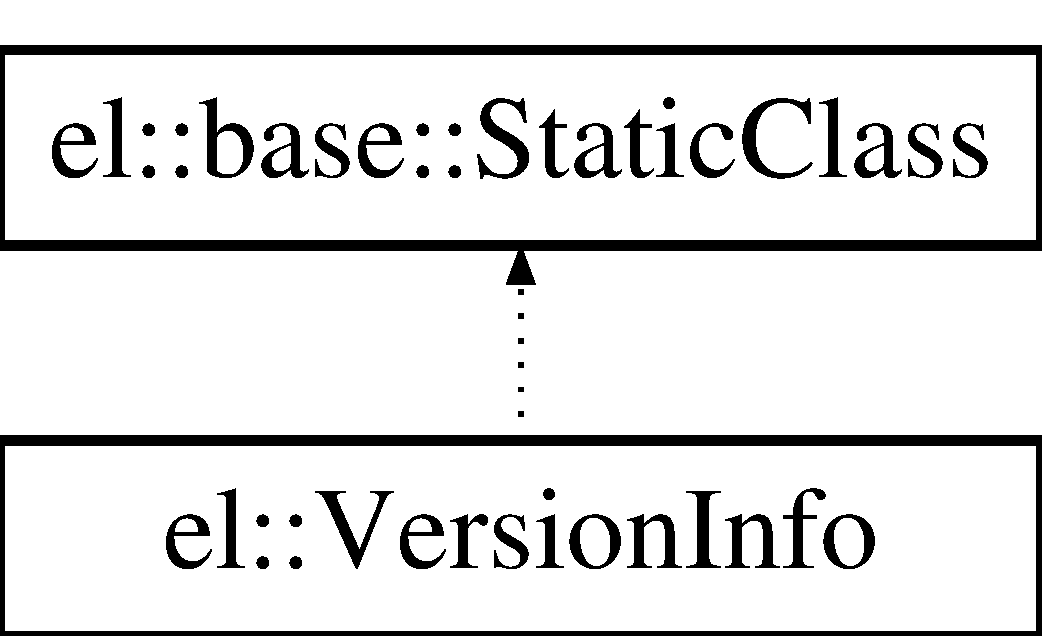
\includegraphics[height=2.000000cm]{classel_1_1VersionInfo}
\end{center}
\end{figure}
\subsection*{Static Public Member Functions}
\begin{DoxyCompactItemize}
\item 
\hypertarget{classel_1_1VersionInfo_a6fee512d52168445b2118ff2b31b4058}{static const std\-::string \hyperlink{classel_1_1VersionInfo_a6fee512d52168445b2118ff2b31b4058}{version} (void)}\label{classel_1_1VersionInfo_a6fee512d52168445b2118ff2b31b4058}

\begin{DoxyCompactList}\small\item\em Current version number. \end{DoxyCompactList}\item 
\hypertarget{classel_1_1VersionInfo_ab23c2545115898f4071fa4e125204946}{static const std\-::string \hyperlink{classel_1_1VersionInfo_ab23c2545115898f4071fa4e125204946}{release\-Date} (void)}\label{classel_1_1VersionInfo_ab23c2545115898f4071fa4e125204946}

\begin{DoxyCompactList}\small\item\em Release date of current version. \end{DoxyCompactList}\end{DoxyCompactItemize}


The documentation for this class was generated from the following file\-:\begin{DoxyCompactItemize}
\item 
/users/disk9/cfse/\-Stage\-\_\-\-Malo/\-C\-P\-A\-C\-S\-Creator\-Lib/\-C\-P\-A\-C\-S\-Creator\-Lib/easylogging++.\-h\end{DoxyCompactItemize}

\hypertarget{classel_1_1base_1_1VRegistry}{\section{el\-:\-:base\-:\-:V\-Registry Class Reference}
\label{classel_1_1base_1_1VRegistry}\index{el\-::base\-::\-V\-Registry@{el\-::base\-::\-V\-Registry}}
}


Represents registries for verbose logging.  




{\ttfamily \#include $<$easylogging++.\-h$>$}

Inheritance diagram for el\-:\-:base\-:\-:V\-Registry\-:\begin{figure}[H]
\begin{center}
\leavevmode
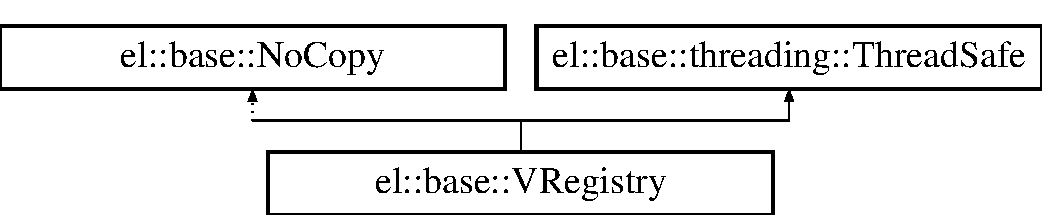
\includegraphics[height=2.000000cm]{classel_1_1base_1_1VRegistry}
\end{center}
\end{figure}
\subsection*{Public Member Functions}
\begin{DoxyCompactItemize}
\item 
\hypertarget{classel_1_1base_1_1VRegistry_ac4b36d32d3722238024480ce66c52ad0}{{\bfseries V\-Registry} (base\-::type\-::\-Verbose\-Level level, base\-::type\-::\-Enum\-Type $\ast$p\-Flags)}\label{classel_1_1base_1_1VRegistry_ac4b36d32d3722238024480ce66c52ad0}

\item 
\hypertarget{classel_1_1base_1_1VRegistry_aea4fb84a03363080ee2501193084f71f}{void \hyperlink{classel_1_1base_1_1VRegistry_aea4fb84a03363080ee2501193084f71f}{set\-Level} (base\-::type\-::\-Verbose\-Level level)}\label{classel_1_1base_1_1VRegistry_aea4fb84a03363080ee2501193084f71f}

\begin{DoxyCompactList}\small\item\em Sets verbose level. Accepted range is 0-\/9. \end{DoxyCompactList}\item 
\hypertarget{classel_1_1base_1_1VRegistry_ad68e225738ecde9a5a59e9fcdfdcc1b9}{base\-::type\-::\-Verbose\-Level {\bfseries level} (void) const }\label{classel_1_1base_1_1VRegistry_ad68e225738ecde9a5a59e9fcdfdcc1b9}

\item 
\hypertarget{classel_1_1base_1_1VRegistry_a52de90db82e57827ac3d3994f70c17cf}{void {\bfseries clear\-Modules} (void)}\label{classel_1_1base_1_1VRegistry_a52de90db82e57827ac3d3994f70c17cf}

\item 
\hypertarget{classel_1_1base_1_1VRegistry_a65e202cc547cd11231d3ea0fb70765d0}{void {\bfseries set\-Modules} (const char $\ast$modules)}\label{classel_1_1base_1_1VRegistry_a65e202cc547cd11231d3ea0fb70765d0}

\item 
\hypertarget{classel_1_1base_1_1VRegistry_a13b725e3da8935fce5cf3c16fd3a2ff9}{bool {\bfseries allowed} (base\-::type\-::\-Verbose\-Level vlevel, const char $\ast$file)}\label{classel_1_1base_1_1VRegistry_a13b725e3da8935fce5cf3c16fd3a2ff9}

\item 
\hypertarget{classel_1_1base_1_1VRegistry_a088456766019a17f5e3fb53ae41abcce}{const std\-::unordered\-\_\-map\\*
$<$ std\-::string, \\*
base\-::type\-::\-Verbose\-Level $>$ \& {\bfseries modules} (void) const }\label{classel_1_1base_1_1VRegistry_a088456766019a17f5e3fb53ae41abcce}

\item 
\hypertarget{classel_1_1base_1_1VRegistry_a811e62d7d016a0714b4363f47216a9da}{void {\bfseries set\-From\-Args} (const \hyperlink{classel_1_1base_1_1utils_1_1CommandLineArgs}{base\-::utils\-::\-Command\-Line\-Args} $\ast$command\-Line\-Args)}\label{classel_1_1base_1_1VRegistry_a811e62d7d016a0714b4363f47216a9da}

\item 
\hypertarget{classel_1_1base_1_1VRegistry_ad7a8e939daf6b3d6b949def0a9f65a1f}{bool \hyperlink{classel_1_1base_1_1VRegistry_ad7a8e939daf6b3d6b949def0a9f65a1f}{v\-Modules\-Enabled} (void)}\label{classel_1_1base_1_1VRegistry_ad7a8e939daf6b3d6b949def0a9f65a1f}

\begin{DoxyCompactList}\small\item\em Whether or not v\-Modules enabled. \end{DoxyCompactList}\end{DoxyCompactItemize}


\subsection{Detailed Description}
Represents registries for verbose logging. 

The documentation for this class was generated from the following file\-:\begin{DoxyCompactItemize}
\item 
/users/disk9/cfse/\-Stage\-\_\-\-Malo/\-C\-P\-A\-C\-S\-Creator\-Lib/\-C\-P\-A\-C\-S\-Creator\-Lib/easylogging++.\-h\end{DoxyCompactItemize}

\hypertarget{classel_1_1base_1_1Writer}{\section{el\-:\-:base\-:\-:Writer Class Reference}
\label{classel_1_1base_1_1Writer}\index{el\-::base\-::\-Writer@{el\-::base\-::\-Writer}}
}


Main entry point of each logging.  




{\ttfamily \#include $<$easylogging++.\-h$>$}

Inheritance diagram for el\-:\-:base\-:\-:Writer\-:\begin{figure}[H]
\begin{center}
\leavevmode
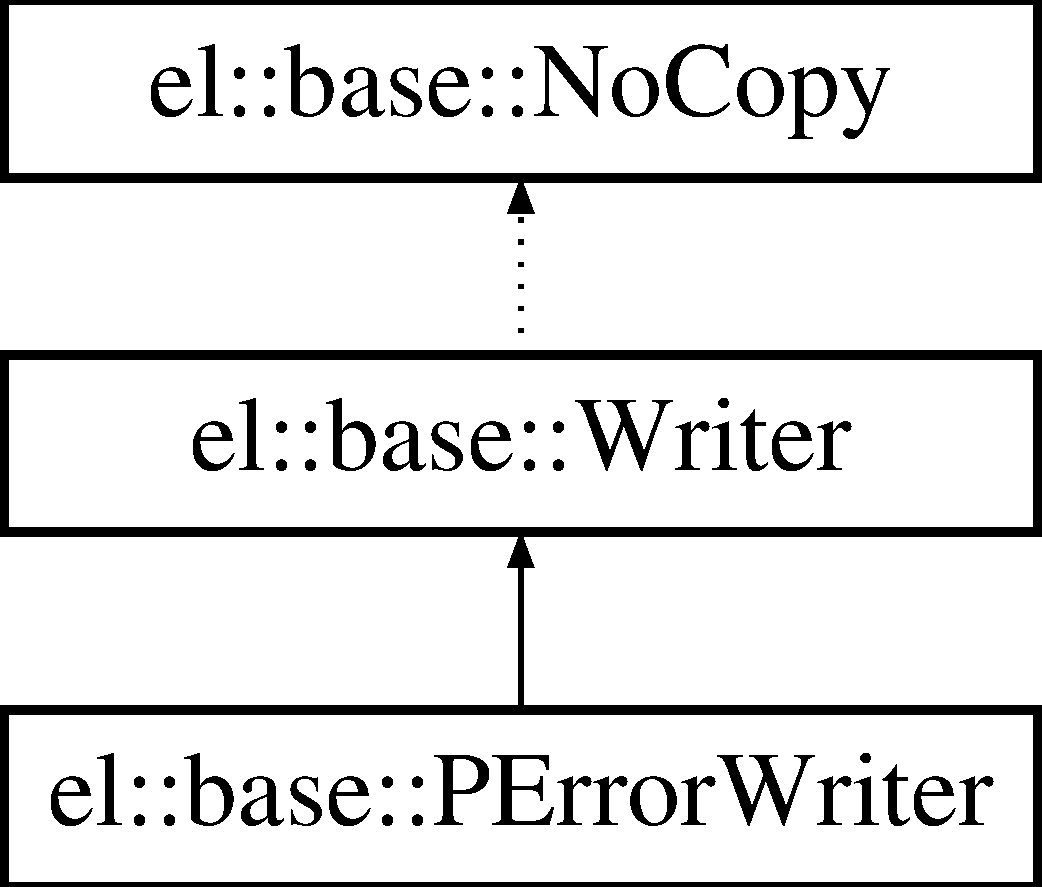
\includegraphics[height=3.000000cm]{classel_1_1base_1_1Writer}
\end{center}
\end{figure}
\subsection*{Public Member Functions}
\begin{DoxyCompactItemize}
\item 
\hypertarget{classel_1_1base_1_1Writer_a50ce36cd8d9e60391da37658623a88a0}{{\bfseries Writer} (\hyperlink{namespaceel_ab0ac6091262344c52dd2d3ad099e8e36}{Level} level, const char $\ast$file, base\-::type\-::\-Line\-Number line, const char $\ast$func, \hyperlink{namespaceel_1_1base_a3aa2563d38e47388ba242a1694fc2839}{base\-::\-Dispatch\-Action} dispatch\-Action=base\-::\-Dispatch\-Action\-::\-Normal\-Log, base\-::type\-::\-Verbose\-Level verbose\-Level=0)}\label{classel_1_1base_1_1Writer_a50ce36cd8d9e60391da37658623a88a0}

\item 
\hypertarget{classel_1_1base_1_1Writer_a5eda18d17eb58ef183d6e36195003be4}{{\bfseries Writer} (\hyperlink{classel_1_1LogMessage}{Log\-Message} $\ast$msg, \hyperlink{namespaceel_1_1base_a3aa2563d38e47388ba242a1694fc2839}{base\-::\-Dispatch\-Action} dispatch\-Action=base\-::\-Dispatch\-Action\-::\-Normal\-Log)}\label{classel_1_1base_1_1Writer_a5eda18d17eb58ef183d6e36195003be4}

\item 
\hypertarget{classel_1_1base_1_1Writer_ab94f0d920c6465a57937e893aa9f5ada}{{\footnotesize template$<$typename T $>$ }\\\hyperlink{classel_1_1base_1_1Writer}{Writer} \& {\bfseries operator$<$$<$} (const T \&log)}\label{classel_1_1base_1_1Writer_ab94f0d920c6465a57937e893aa9f5ada}

\item 
\hypertarget{classel_1_1base_1_1Writer_aea6d7f996ff92e9485a76ad3955f0a29}{\hyperlink{classel_1_1base_1_1Writer}{Writer} \& {\bfseries operator$<$$<$} (std\-::ostream \&($\ast$log)(std\-::ostream \&))}\label{classel_1_1base_1_1Writer_aea6d7f996ff92e9485a76ad3955f0a29}

\item 
\hypertarget{classel_1_1base_1_1Writer_ac518e6b23327127f63c6d26ee83ecbf9}{{\bfseries operator bool} ()}\label{classel_1_1base_1_1Writer_ac518e6b23327127f63c6d26ee83ecbf9}

\item 
\hypertarget{classel_1_1base_1_1Writer_a282d82f392a3e6fef9eda47ce53e87dc}{\hyperlink{classel_1_1base_1_1Writer}{Writer} \& {\bfseries construct} (\hyperlink{classel_1_1Logger}{Logger} $\ast$logger, bool need\-Lock=true)}\label{classel_1_1base_1_1Writer_a282d82f392a3e6fef9eda47ce53e87dc}

\item 
\hypertarget{classel_1_1base_1_1Writer_ab2bc960787eb3c9b01569629dcbeb246}{\hyperlink{classel_1_1base_1_1Writer}{Writer} \& {\bfseries construct} (int count, const char $\ast$logger\-Ids,...)}\label{classel_1_1base_1_1Writer_ab2bc960787eb3c9b01569629dcbeb246}

\end{DoxyCompactItemize}
\subsection*{Protected Member Functions}
\begin{DoxyCompactItemize}
\item 
\hypertarget{classel_1_1base_1_1Writer_ae687ebbee62b086f318ee4c8d1a655c4}{void {\bfseries initialize\-Logger} (const std\-::string \&logger\-Id, bool lookup=true, bool need\-Lock=true)}\label{classel_1_1base_1_1Writer_ae687ebbee62b086f318ee4c8d1a655c4}

\item 
\hypertarget{classel_1_1base_1_1Writer_a692d05d209840d6ae8c2c8e0bea21d29}{void {\bfseries process\-Dispatch} ()}\label{classel_1_1base_1_1Writer_a692d05d209840d6ae8c2c8e0bea21d29}

\item 
\hypertarget{classel_1_1base_1_1Writer_a1c7d90bd4e00af4e7307f5936e1b6507}{void {\bfseries trigger\-Dispatch} (void)}\label{classel_1_1base_1_1Writer_a1c7d90bd4e00af4e7307f5936e1b6507}

\end{DoxyCompactItemize}
\subsection*{Protected Attributes}
\begin{DoxyCompactItemize}
\item 
\hypertarget{classel_1_1base_1_1Writer_aad87d889b6ad94bcbf4fd01ca33c47d4}{\hyperlink{classel_1_1LogMessage}{Log\-Message} $\ast$ {\bfseries m\-\_\-msg}}\label{classel_1_1base_1_1Writer_aad87d889b6ad94bcbf4fd01ca33c47d4}

\item 
\hypertarget{classel_1_1base_1_1Writer_a28522bf9b05b4edcc0baf5196645d317}{\hyperlink{namespaceel_ab0ac6091262344c52dd2d3ad099e8e36}{Level} {\bfseries m\-\_\-level}}\label{classel_1_1base_1_1Writer_a28522bf9b05b4edcc0baf5196645d317}

\item 
\hypertarget{classel_1_1base_1_1Writer_a1eada1175721ba11b4eb6c9515d8e2dc}{const char $\ast$ {\bfseries m\-\_\-file}}\label{classel_1_1base_1_1Writer_a1eada1175721ba11b4eb6c9515d8e2dc}

\item 
\hypertarget{classel_1_1base_1_1Writer_aae6f7c08c2617a5ba1ffc38d4eb53207}{const base\-::type\-::\-Line\-Number {\bfseries m\-\_\-line}}\label{classel_1_1base_1_1Writer_aae6f7c08c2617a5ba1ffc38d4eb53207}

\item 
\hypertarget{classel_1_1base_1_1Writer_a57291e0751fe93547d9d5551fb3e8415}{const char $\ast$ {\bfseries m\-\_\-func}}\label{classel_1_1base_1_1Writer_a57291e0751fe93547d9d5551fb3e8415}

\item 
\hypertarget{classel_1_1base_1_1Writer_a335803052b6878c058a4a888279df04d}{base\-::type\-::\-Verbose\-Level {\bfseries m\-\_\-verbose\-Level}}\label{classel_1_1base_1_1Writer_a335803052b6878c058a4a888279df04d}

\item 
\hypertarget{classel_1_1base_1_1Writer_a0fab2e9a168b7973bcca4574d05490d2}{\hyperlink{classel_1_1Logger}{Logger} $\ast$ {\bfseries m\-\_\-logger}}\label{classel_1_1base_1_1Writer_a0fab2e9a168b7973bcca4574d05490d2}

\item 
\hypertarget{classel_1_1base_1_1Writer_a238593eda90cf32645c4541e738bea9a}{bool {\bfseries m\-\_\-proceed}}\label{classel_1_1base_1_1Writer_a238593eda90cf32645c4541e738bea9a}

\item 
\hypertarget{classel_1_1base_1_1Writer_a63763a047d595271cb14f9a80430306b}{\hyperlink{classel_1_1base_1_1MessageBuilder}{base\-::\-Message\-Builder} {\bfseries m\-\_\-message\-Builder}}\label{classel_1_1base_1_1Writer_a63763a047d595271cb14f9a80430306b}

\item 
\hypertarget{classel_1_1base_1_1Writer_acbea5b77953cf6e39baab015e83a4100}{\hyperlink{namespaceel_1_1base_a3aa2563d38e47388ba242a1694fc2839}{base\-::\-Dispatch\-Action} {\bfseries m\-\_\-dispatch\-Action}}\label{classel_1_1base_1_1Writer_acbea5b77953cf6e39baab015e83a4100}

\item 
\hypertarget{classel_1_1base_1_1Writer_a9137860437510e1a26e8b0c1814c7ae7}{std\-::vector$<$ std\-::string $>$ {\bfseries m\-\_\-logger\-Ids}}\label{classel_1_1base_1_1Writer_a9137860437510e1a26e8b0c1814c7ae7}

\end{DoxyCompactItemize}
\subsection*{Friends}
\begin{DoxyCompactItemize}
\item 
\hypertarget{classel_1_1base_1_1Writer_a2fb8a2c02cbf86247f093c118bed877a}{class {\bfseries el\-::\-Helpers}}\label{classel_1_1base_1_1Writer_a2fb8a2c02cbf86247f093c118bed877a}

\end{DoxyCompactItemize}


\subsection{Detailed Description}
Main entry point of each logging. 

The documentation for this class was generated from the following file\-:\begin{DoxyCompactItemize}
\item 
/users/disk9/cfse/\-Stage\-\_\-\-Malo/\-C\-P\-A\-C\-S\-Creator\-Lib/\-C\-P\-A\-C\-S\-Creator\-Lib/easylogging++.\-h\end{DoxyCompactItemize}

\chapter{File Documentation}
\hypertarget{Point_8cpp}{\section{/users/disk9/cfse/\-Stage\-\_\-\-Malo/\-C\-P\-A\-C\-S\-Creator\-Lib/\-C\-P\-A\-C\-S\-Creator\-Lib/\-Point.cpp File Reference}
\label{Point_8cpp}\index{/users/disk9/cfse/\-Stage\-\_\-\-Malo/\-C\-P\-A\-C\-S\-Creator\-Lib/\-C\-P\-A\-C\-S\-Creator\-Lib/\-Point.\-cpp@{/users/disk9/cfse/\-Stage\-\_\-\-Malo/\-C\-P\-A\-C\-S\-Creator\-Lib/\-C\-P\-A\-C\-S\-Creator\-Lib/\-Point.\-cpp}}
}


Implementation of a T\-I\-G\-L point.  


{\ttfamily \#include \char`\"{}Point.\-h\char`\"{}}\\*
{\ttfamily \#include $<$math.\-h$>$}\\*
{\ttfamily \#include $<$vector$>$}\\*
\subsection*{Namespaces}
\begin{DoxyCompactItemize}
\item 
\hyperlink{namespacecpcr}{cpcr}
\begin{DoxyCompactList}\small\item\em Structure element to hold the C\-P\-A\-C\-S tree. \end{DoxyCompactList}\end{DoxyCompactItemize}


\subsection{Detailed Description}
Implementation of a T\-I\-G\-L point. modification of tigl class 
\hypertarget{Point_8h}{\section{/users/disk9/cfse/\-Stage\-\_\-\-Malo/\-C\-P\-A\-C\-S\-Creator\-Lib/\-C\-P\-A\-C\-S\-Creator\-Lib/\-Point.h File Reference}
\label{Point_8h}\index{/users/disk9/cfse/\-Stage\-\_\-\-Malo/\-C\-P\-A\-C\-S\-Creator\-Lib/\-C\-P\-A\-C\-S\-Creator\-Lib/\-Point.\-h@{/users/disk9/cfse/\-Stage\-\_\-\-Malo/\-C\-P\-A\-C\-S\-Creator\-Lib/\-C\-P\-A\-C\-S\-Creator\-Lib/\-Point.\-h}}
}


Implementation of a C\-P\-R\-E\-A\-T\-O\-R point. More or less imported from the T\-I\-G\-L\-Point without the oce feature.  


{\ttfamily \#include $<$climits$>$}\\*
{\ttfamily \#include $<$iostream$>$}\\*
{\ttfamily \#include $<$vector$>$}\\*
{\ttfamily \#include $<$Eigen/\-Dense$>$}\\*
\subsection*{Classes}
\begin{DoxyCompactItemize}
\item 
class \hyperlink{classcpcr_1_1Point}{cpcr\-::\-Point}
\end{DoxyCompactItemize}
\subsection*{Namespaces}
\begin{DoxyCompactItemize}
\item 
\hyperlink{namespacecpcr}{cpcr}
\begin{DoxyCompactList}\small\item\em Structure element to hold the C\-P\-A\-C\-S tree. \end{DoxyCompactList}\end{DoxyCompactItemize}


\subsection{Detailed Description}
Implementation of a C\-P\-R\-E\-A\-T\-O\-R point. More or less imported from the T\-I\-G\-L\-Point without the oce feature. 
%--- End generated contents ---

% Index
\newpage
\phantomsection
\addcontentsline{toc}{part}{Index}
\printindex

\end{document}
